\documentclass[12pt,a4paper,twoside,french,openright]{book}
\makeatletter
\let\latex@include\include
\def\include#1{\include@aux#1\@nil}
\def\include@aux#1/#2\@nil{\@mkdir{#1}\latex@include{#1/#2}}
\ifnum\pdfshellescape=\@ne
\def\@mkdir#1{\immediate\write18{mkdir -p ./build/#1}}
\else
\def\@mkdir{\typeout{Expect errors}}
\fi
\makeatother 
\hyphenpenalty=3500
\doublehyphendemerits=9000
\finalhyphendemerits=6000
\RequirePackage[l2tabu, orthodox]{nag}
\usepackage{textcomp}
\usepackage{afterpage,everypage}
\usepackage{pdflscape}
\usepackage{rotating}
\usepackage{float}
\usepackage{amsmath}
\usepackage{physics}
\usepackage{cmap}
\usepackage[T1]{fontenc}
\usepackage[french]{babel}
\usepackage{enumitem}
\usepackage[utf8]{inputenc}
\usepackage{caption}
\usepackage{collcell}
\usepackage{booktabs}
\usepackage{xcolor,colortbl}
\usepackage[backend=biber,style=numeric,sorting=none,hyperref=true]{biblatex}
\usepackage{csquotes}
\usepackage{cellspace}
\cellspacetoplimit=4pt
\cellspacebottomlimit=4pt
\usepackage{minipage-marginpar}
\usepackage{calc}
\usepackage{lmodern}
\usepackage{microtype}
\usepackage[top=2.05cm,bottom=1.1cm,left=1cm,right=5cm,marginparsep=0.50cm,marginparwidth=4.25cm,headheight=25pt]{geometry}
\usepackage{booktabs}
\usepackage{layout}
\usepackage{graphicx}
\usepackage{makecell}
\usepackage{titlesec}
\usepackage{setspace}
\usepackage{pgf}
\usepackage{soul}
\usepackage[outline]{contour}
\usepackage{eqnarray}
\usepackage{tikz}
\usepackage{lscape}
\usepackage{url}
\usepackage[subfigure]{tocloft}
\setlength{\cftfignumwidth}{3em}
\usepackage{fancyhdr}
\usepackage{blindtext}
\usepackage{wrapfig}
\usepackage{cutwin}
\usepackage{framed}
\usepackage{colortbl}
\usepackage{tabularx}
\usepackage{amssymb,mathrsfs}
\usepackage{makeidx}
\usepackage{lettrine}
\usepackage{coffee4}
\usepackage{fancybox}
\usepackage[lofdepth,lotdepth]{subfig}
\usepackage{multirow}
\usepackage{multicol}
\usepackage{graphicx}
\usepackage{eso-pic}
\usepackage{lipsum}
\usepackage[Bjornstrup]{fncychap}
\usepackage{hyperref}
%%% --- The following two lines are what needs to be added --- %%%
\setcounter{biburllcpenalty}{7000}
\setcounter{biburlucpenalty}{8000}
\usepackage[all]{hypcap}
\usepackage[french,tight]{minitoc}
\hypersetup{colorlinks=true,breaklinks=true,bookmarksopen=true,urlcolor=gray,citecolor=gray,linkcolor=gray}                                                    
\setlength{\fboxsep}{0mm}
\renewcommand {\mtctitle} {}
\usepackage{ifthen}
\usepackage{marginnote}
\usepackage{chngpage}
\usepackage{pdfcomment}
\usepackage{feynmp}
\usepackage{marginfit}
\usepackage[mode=build]{standalone}
\usepackage{pgfplots}
\usepackage{wallpaper}
\pgfplotsset{width=10cm,compat=newest}
\usepackage{silence}
\WarningFilter{Fancyhdr}{\headheight is too small}
\usepackage[tight]{shorttoc}
\usepackage{chemist}
\usepackage{listing}

\pgfplotsset{compat=newest}
\usepgfplotslibrary{external,colormaps} 
%\tikzexternalize
\tikzset{%
	external/force remake=false,
	/tikz/external/optimize=false,
	external/system call={pdflatex \tikzexternalcheckshellescape --halt-on-error --interaction=batchmode --output-directory=./build --jobname "\image" "\texsource"},
	/pgf/images/include external/.code={%
		\includegraphics{build/#1}%
	},
}

% Define the command. Note that the input and output folders are static!
\newcommand{\includetex}[1]
{%
	\tikzsetnextfilename{#1}%
	\input{#1.tex}%
}

\usepackage{ifthen}
\newcommand{\Cpp}[1][]{$\text{C\hspace{-.25ex}}^{_{_{_{++}}}}\ifthenelse{\equal{#1}{}}{}{\text{\hspace{-.625ex}#1}}$}
\newcommand*\diff{\mathop{}\!\mathrm{d}}
\newcommand*\Diff[1]{\mathop{}\!\mathrm{d^#1}}
\usepackage{tocbibind}
%\DeclareMathSymbol{\Omega}{\mathalpha}{letters}{"0A}% italics
\DeclareMathSymbol{\varOmega}{\mathalpha}{operators}{"0A}% upright
\providecommand*{\upOmega}{\varOmega}% for siunitx
\usepackage[binary-units=true]{siunitx}
\sisetup{locale = FR}
\DeclareSIUnit{\bits}{bits}
\DeclareSIUnit{\hit}{Hits}
\DeclareSIUnit{\hitt}{Hit}
\DeclareSIUnit{\strip}{Strip}
\DeclareSIUnit\sq{\ensuremath{\Box}}
\DeclareSIUnit\clusters{cluster}
\DeclareSIUnit{\c}{c}

\DeclareFontShape{OT1}{cmr}{bx}{sc}{<-> cmbcsc10}{}
%"Bugfix" for fncychap:
%Without this code there will be an overfull hbox by 10pt on every chapter
%I don't remember where I found this, but it seems to be unrelated to 
%the problem sice the header looks the same when commented out.     
%--------------------------------------------------------------------------
\renewcommand{\DOCH}{%
	\settowidth{\py}{\CNoV\thechapter}
	%\addtolength{\py}{-2pt}      % Amount of space by which the
	%                                % number is shifted right
	\fboxsep=0pt%
	\colorbox[gray]{.85}{\rule{0pt}{40pt}\parbox[b]{\textwidth}{\hfill}}%
	\kern-\py\raise20pt%
	\hbox{\color[gray]{.5}\CNoV\thechapter}\\%
}

\makeatletter
\newcommand{\listequation}[2]{$\displaystyle #1$\hfill\refstepcounter{equation}\label{#2}\textup{\tagform@{\theequation}}}
\makeatother



\SetProtrusion{encoding={*},family={*},series={*},size={6,7,8}}{1={ ,750},2={ ,500},3={ ,500},4={ ,500},5={ ,500},6={ ,500},7={ ,600},8={ ,500},9={ ,500},0={ ,500}}
\microtypecontext{kerning=french}
\usetikzlibrary{calc,positioning,shadows.blur,decorations.pathreplacing,shapes,positioning,patterns,plotmarks}
\usepackage{etoolbox}
\newcolumntype{Y}[1]{>{\centering\arraybackslash}p{#1}<{\centering\arraybackslash}}
\newcolumntype{L}{>{\arraybackslash\vspace{0.1cm}}Cc<{\vspace{0.1cm}\arraybackslash}}
\newcolumntype{O}{>{\centering\arraybackslash}Cc<{\centering\arraybackslash}}
\newcolumntype{N}{@{}m{0pt}@{}}
%%%%%Use titlesec to color section subsection subsubsection
\newcommand{\ColorSection}[1]{\colorbox{black!65}{\parbox[c][1.5em][c]{\dimexpr\textwidth-2\fboxsep}{\hspace{0.2cm}\textcolor{white}{\thesection\ #1}\hspace*{0.5cm}}}}
\titleformat{\section}{\rmfamily\large\raggedright}{}{0pt}{\ColorSection}     
\titleformat{name=\section,numberless}{\rmfamily\large\raggedright}{}{0pt}{\ColorSection}       
\newcommand{\ColorSubSection}[1]{\colorbox{black!65}{\parbox[c][1.5em][c]{\dimexpr\textwidth-2\fboxsep}{\hspace{0.2cm}\textcolor{white}{\thesubsection\ #1}\hspace*{0.5cm}}}}
\titleformat{\subsection}{\rmfamily\raggedright}{}{0pt}{\ColorSubSection}     
\titleformat{name=\subsection,numberless}{\rmfamily\raggedright}{}{0pt}{\ColorSubSection}       
\newcommand{\ColorSubSubSection}[1]{\colorbox{black!55}{\parbox[c][1.5em][c]{\dimexpr\textwidth-2\fboxsep}{\hspace{0.2cm}\textcolor{white}{\thesubsubsection\ #1}\hspace*{0.5cm}}}}
\titleformat{\subsubsection}{\rmfamily\raggedright}{}{0pt}{\ColorSubSubSection}
\titleformat{name=\subsubsection,numberless}{\rmfamily\raggedright}{}{0pt}{\ColorSubSubSection}   
%%%%%%%%%%%%%%%%%%%%%%%%%%%%%%%%%%%%%%%%%%%%%%%%%%%%%%%%%%%
\titlespacing*{\section}{0pt}{\baselineskip}{\baselineskip}
\titlespacing*{\subsection}{0pt}{\baselineskip}{\baselineskip}
\titlespacing*{\subsubsection}{0pt}{\baselineskip}{\baselineskip}
\newlength{\mylength}
\setlength{\mylength}{\textheight+\headsep-\paperheight}

\makeatletter
\newlength\myrightmargin
\setlength\myrightmargin{\Gm@rmargin}
\newlength\mymarge
\setlength\mymarge{0.45\textwidth}
\makeatother 

\newcommand{\void}{\vspace*{\paperheight}\textcolor{gray!30}{\hrule}}
\newcommand{\leftnum}{\vspace*{\paperheight}\textcolor{white}{\hrule}\vspace{0.2cm}\makebox[\textwidth][l]{\hspace{0.5cm}\sffamily\textcolor{white}{ \large{\thepage}}}\vspace{0.5cm}}
\newcommand{\rightnum}{\vspace*{\paperheight}\textcolor{white}{\hrule}\vspace{0.2cm}\makebox[\textwidth][r]{\sffamily\textcolor{white}{ \large{\thepage}}\hspace{0.5cm}}\vspace{0.5cm}}

\newcommand{\MargeSimple}[2]
{%
	\ClearShipoutPicture
	\AddToShipoutPicture{%
		\ifthenelse{\isodd{\value{page}}}{
			\AtPageLowerRight{%
				{\colorbox{gray!30}{%
						\begin{minipage}[b]{\dimexpr\myrightmargin-0.5\marginparsep\relax}
							\vspace*{\paperheight}
							#2
						\end{minipage}%
				}}%
			}%
		}
		{
			\AtPageLowerLeft{%
				{\colorbox{gray!30}{%
						\begin{minipage}[b]{\dimexpr\myrightmargin-0.5\marginparsep\relax}
							\vspace*{\paperheight}
							#1
						\end{minipage}%
				}}%
			}%
		}
	}
    %\ClearShipoutPicture
}
\newcommand{\rien}
{%
	\ClearShipoutPicture
	\AddToShipoutPicture{}
}

\mtcsetdepth{minitoc}{2}
\mtcsettitle{minitoc}{Contenu :}
\usepackage{listings}
\usepackage{cleveref} %GEEENIAAAAL!!!
%\let\oldfootnotesize\footnotesize
%\renewcommand*{\footnotesize}{\oldfootnotesize\fontsize{5}{7}}

\captionsetup{justification=raggedright,labelfont={color=gray,bf,small},font=small}

\newcommand{\ligne}{\color{gray}{\rule{\linewidth}{5pt}}\vspace{0.2cm}\color{black}}

\makeatletter
\newcommand\At@Page@Upper@Right[1]{%
  \put(\LenToUnit{\paperwidth},\LenToUnit{\paperheight}){#1}%
}
\newcommand\AtPageLowerRight[1]{\At@Page@Upper@Right{%
  \put(0,\LenToUnit{-\paperheight}){\llap{#1}}}}
\makeatother

\renewcommand{\contentsname}{Table des matières}
\renewcommand{\thechapter}{\arabic{chapter}}
\renewcommand{\thesection}{\arabic{section}}
\renewcommand{\thesubsection}{\thesection.\arabic{subsection}}
\renewcommand{\thesubsubsection}{}

%% Command to hold chapter illustration image
\newcommand\chapterillustration{}
\titlespacing*{\chapter}{0pt}{0pt}{135mm}

\newcommand{\repeatcaption}[2]{%
  \addtocounter{figure}{-1}%
  \renewcommand{\thefigure}{\ref{#1}}%
  \captionsetup{list=no, labelformat=simple, labelsep=colon}%
  \captionof{figure}{#2}%
}

\newcommand{\repeatsubcaption}[2]{%
  \renewcommand{\thesubfigure}{\subref{#1}}%
  \captionsetup{list=no, labelformat=parens, labelsep=space}%
  \captionof{subfigure}{#2}%
}

%%%%********************************************************************
% fancy quotes
\definecolor{quotemark}{gray}{0.7}
\makeatletter
\def\fquote{%
    \@ifnextchar[{\fquote@i}{\fquote@i[]}%]
}%
\def\fquote@i[#1]{%
    \def\tempa{#1}%
    \@ifnextchar[{\fquote@ii}{\fquote@ii[]}%]
}%
\def\fquote@ii[#1]{%
    \def\tempb{#1}%
    \@ifnextchar[{\fquote@iii}{\fquote@iii[]}%]
}%
\def\fquote@iii[#1]{%
    \def\tempc{#1}%
    \@ifnextchar[{\fquote@iiii}{\fquote@iiii[]}%]
}%
\def\fquote@iiii[#1]{%
    \def\tempd{#1}%
    \vspace{1em}%
    \noindent%
    \begin{list}{}
    {%
    		\setlength{\leftmargin}{0.1\textwidth}%
      \setlength{\rightmargin}{0.1\textwidth}%
    }%
    \item[]%
    \begin{picture}(0,0)%
    \put(\tempd,-15){\makebox(0,0){\scalebox{3}{\textcolor{quotemark}{``}}}}%
    \end{picture}%
    \begingroup\itshape
 }%
 %%%%********************************************************************
 \def\endfquote
 {%
    %\vspace*{0.15cm}
 	\endgroup\par%
 	\makebox[0pt][l]{%
 	\hspace{0.8\textwidth}%
 	\vspace{0.1cm}%
 	\begin{picture}(0,0)(0,0)%
 	\put(15,8){\makebox(0,0){\scalebox{3}{\color{quotemark}''}}}%
 	\end{picture}}%
 	\ifx\tempa\empty%
 	\else%
  \ifx\tempb\empty%
  \hfill\mbox{}\hfill\tempa%
  \else%
  \ifx\tempc\empty%
  \hfill\mbox{}\hfill\tempa,\ \emph{\tempb}%
  \else%
  \hfill\mbox{}\hfill\tempa,\ \emph{\tempb},\ \tempc%
  \fi\fi\fi\par%
  \vspace{0.7em}%
 	\end{list}%
 }%
 \makeatother
 %%%%********************************************************************
%\mtcsetfeature{minitoc}{open}{\vspace{-1.5cm}}
\setcounter{tocdepth}{3}
\makeindex

\renewcommand{\LettrineFontHook}{\color{gray}}
\usepackage{yfonts}

\newcommand{\lettrines}[2]{\lettrine[lines=2, slope= -0.5em, lhang=0.25, loversize=0.25]{#1}{\small #2}}

\makeatletter
\renewcommand{\fnum@figure}{Fig. \thefigure}
\makeatother

\interfootnotelinepenalty=10000
\setlength{\parskip}{\baselineskip}
\addbibresource{bibli.bib}

\renewcommand{\headrulewidth}{0pt}
\renewcommand{\footrulewidth}{0pt}
\fancypagestyle{plain}{\fancyhf{}\fancyhead{}\renewcommand{\headrulewidth}{0pt}} 
\fancypagestyle{void}{\fancyhf{}\fancyhead{}\renewcommand{\headrulewidth}{0pt}} 

\definecolor{shadecolor}{gray}{0.75}

\newcommand{\balajipage}[1]{\fboxsep=0pt\colorbox{shadecolor}{\balajistrut\makebox[#1][c]{}}}
\newcommand{\balajihead}[1]{\fboxsep=0pt\colorbox{shadecolor}{\balajistrut\makebox[\textwidth][s]{#1}}}

\newcommand{\balajistrut}{%
	\vrule width 0pt 
	height 1.5\ht\strutbox 
	depth 1.5\dp\strutbox
}
\newlength{\mylengthh}
\fancypagestyle{mystyle}
{
	\fancyhf{} 
	\fancyhead[RE,RO]{}
	\fancyheadoffset[LE,RO]{\marginparsep+\marginparwidth}
	\setlength{\mylengthh}{\widthof{\fontsize{55}{10}\selectfont \hbox{\color[gray]{.5}\CNoV\thechapter}}}
	\fancyhead[LO]
	{%
		\begin{minipage}{\textwidth}
			\balajihead{\quad\bfseries\color{white}\textbf{\leftmark}\hfill}%
			\hspace*{-1\mylengthh}
			\noindent
			\begin{minipage}{\widthof{\fontsize{55}{10}\selectfont \hbox{\color[gray]{.5}\CNoV\thechapter}}}
				\vspace*{-0.30cm}
				\fontsize{55}{10}\selectfont \hbox{\color[gray]{.5}\CNoV\thechapter}
			\end{minipage}%
			\hspace*{-0.16\mylengthh}
			\makebox[\myrightmargin][r]{\balajipage{\dimexpr\myrightmargin-0.5\marginparsep\relax}}%
		\end{minipage}
	}
	\fancyhead[LE]
	{%
		\begin{minipage}{\textwidth}
			\hspace*{-0.78\marginparsep}
			\makebox[\myrightmargin][l]{\balajipage{\dimexpr\myrightmargin-0.5\marginparsep\relax}}%
			\balajihead{\hfill\bfseries\color{white}\textbf{\leftmark}\quad}%
			\hspace*{-\textwidth}
			\noindent
			\begin{minipage}{\widthof{\fontsize{55}{10}\selectfont \hbox{\color[gray]{.5}\CNoV\thechapter}}}
				\vspace*{-0.30cm}
				\fontsize{55}{10}\selectfont \hbox{\color[gray]{.5}\CNoV\thechapter}
			\end{minipage}%
		\end{minipage}
	}
	\fancyfoot[RO]{}
	\fancyfoot[LE]{}
}

\makeatletter
\newif\if@nothing
\@nothingtrue
\newif\if@backmatter
\@backmatterfalse
\newif\if@frontmatter
\@frontmatterfalse
\newif\if@supress
\@supressfalse
\renewcommand\frontmatter{\cleardoublepage\@nothingfalse\@mainmatterfalse\@frontmattertrue\@backmatterfalse\pagenumbering{roman}}
\renewcommand\mainmatter{\cleardoublepage\@nothingfalse\@mainmattertrue\@frontmatterfalse\@backmatterfalse\pagenumbering{arabic}}
\renewcommand\backmatter{\if@openright\cleardoublepage\else\clearpage\fi\@nothingfalse\@mainmatterfalse\@frontmatterfalse\@backmattertrue}
\newcommand{\nothing}{\cleardoublepage\@nothingtrue\@mainmatterfalse\@frontmatterfalse\@backmatterfalse\pagenumbering{roman}}
\newcommand{\reset}{\cleardoublepage\@nothingfalse\@mainmatterfalse\@frontmatterfalse\@backmatterfalse\pagenumbering{roman}}
\AddEverypageHook{%
	\if@nothing
		\pagestyle{void}
		\rien{}
	\else
		\if@supress
		    \MargeSimple{\void}{\void}
		    \pagestyle{void}
		\else
			\if@mainmatter
				\MargeSimple{\leftnum}{\rightnum}
			\else
				\if@frontmatter
					\MargeSimple{\leftnum}{\rightnum}
				\else
					\if@backmatter
						\MargeSimple{\void}{\void}
					\else
				     	\pagestyle{void}
			    	 	\rien{}
					\fi
				\fi
			\fi
		\fi
	\fi
}
\makeatother

\makeatletter
\def\cleardoublepage{\@supresstrue\clearpage\if@twoside \ifodd\c@page\else\hbox{}\newpage\if@twocolumn\hbox{}\newpage\fi\fi\fi\@supressfalse}
\makeatother

\begin{document}
\pagestyle{void}
\nothing{}
%%%%%%%%%%%%%%%%%%%%%%%%%%%%%%%%%
% Page de garde %%%%%%%%%%%%
%%%%%%%%%%%%%%%%%%%%%%%%%%%%%%%%%
\setcounter{page}{-1}
\begin{titlepage}	
	\setcounter{page}{-1}
	%%%%%%%%%%%%%%%%
% modèle de page de garde pour une thèse de l'Université de Lyon (version de mars 2016)
% Attention ! Encodage UTF8 ! Sinon adapter en conséquence...
%%%%%%%%%%%%%%%%
	\newgeometry{inner=2.5cm,outer=2.5cm, top=2.5cm, bottom=2.5cm}
	\fancyhf{}
	\setlength{\parindent}{0pt}
	\thispagestyle{empty}
	\begin{center}
		
\includegraphics[height=3cm]{PG/logo.png} %le fichier "logo" doit être dans le même dossier que le fichier tex
	\end{center}
	\vspace{-0.5cm}
	\fontsize{11pt}{13pt}\selectfont
	N\textsuperscript{o} d'ordre NNT : xxx
	
	\vspace{0.5cm}
	
	\begin{center}
		\fontsize{14pt}{16pt}\selectfont
		\textbf{\uppercase{Thèse de doctorat de l'université de Lyon}}\\
		\fontsize{12pt}{14pt}\selectfont
		opérée au sein de\\
		\textbf{l'Université Claude Bernard Lyon 1}
		
		\vspace{0.25cm}
		
		\textbf{École Doctorale ED52\\ École doctorale de Physique et d’Astrophysique (PHAST)}% nom complet de l'école doctorale
		
		\vspace{0.25cm}
		\textbf{Spécialité de doctorat : Physique des Particules}
		\vspace{0.25cm}
		
		Soutenue publiquement le jj/mm/aaaa, par :\\
		\fontsize{14pt}{16pt}\selectfont
		\textbf{François Sylvain René LAGARDE}
	  
		\rule[20pt]{\textwidth}{0.5pt}
		\fontsize{23pt}{26pt}\selectfont
		\textbf{Caractérisation de détecteurs à plaques résistives de verres de basse résistivité en vue de la mise à niveau de CMS}
		\rule{\textwidth}{0.5pt}

	\end{center}
	
	{\fontsize{12pt}{14pt}\selectfont
	Devant le jury composé de :\\}
	{\fontsize{11pt}{13pt}\selectfont

	Nom Prénom, grade/qualité, établissement/entreprise \hfill Président(e)\\ % mention "président" à ne préciser qu'après la 

	Nom Prénom, grade/qualité, établissement/entreprise \hfill Rapporteur(e)\\
	Nom Prénom, grade/qualité, établissement/entreprise \hfill Rapporteur(e)\\
	Nom Prénom, grade/qualité, établissement/entreprise \hfill Examinateur/trice\\
	Nom Prénom, grade/qualité, établissement/entreprise \hfill Examinateur/trice\\
	
	Grenier Gérald, grade/qualité, établissement/entreprise \hfill Directeur de thèse\\
	Gouzevitch Maxime, grade/qualité, établissement/entreprise \hfill Co-directeur de thèse\\
	Nom Prénom, grade/qualité, établissement/entreprise \hfill Invité(e)} % le cas échéant
	\cleardoublepage
	\restoregeometry
\end{titlepage}
\setcounter{page}{-1}
\shipout\null
\shipout\null
\begin{titlepage}	
	%%%%%%%%%%%%%%%%
% modèle de page de garde pour une thèse de l'Université de Lyon (version de mars 2016)
% Attention ! Encodage UTF8 ! Sinon adapter en conséquence...
%%%%%%%%%%%%%%%%
	\newgeometry{inner=2.5cm,outer=2.5cm, top=2.5cm, bottom=2.5cm}
	\fancyhf{}
	\setlength{\parindent}{0pt}
	\thispagestyle{empty}
	\begin{center}
		
\includegraphics[height=3cm]{PG/logo.png} %le fichier "logo" doit être dans le même dossier que le fichier tex
	\end{center}
	\vspace{-0.5cm}
	\fontsize{11pt}{13pt}\selectfont
	N\textsuperscript{o} d'ordre NNT : xxx
	
	\vspace{0.5cm}
	
	\begin{center}
		\fontsize{14pt}{16pt}\selectfont
		\textbf{\uppercase{Thèse de doctorat de l'université de Lyon}}\\
		\fontsize{12pt}{14pt}\selectfont
		opérée au sein de\\
		\textbf{l'Université Claude Bernard Lyon 1}
		
		\vspace{0.25cm}
		
		\textbf{École Doctorale ED52\\ École doctorale de Physique et d’Astrophysique (PHAST)}% nom complet de l'école doctorale
		
		\vspace{0.25cm}
		\textbf{Spécialité de doctorat : Physique des Particules}
		\vspace{0.25cm}
		
		Soutenue publiquement le jj/mm/aaaa, par :\\
		\fontsize{14pt}{16pt}\selectfont
		\textbf{François Sylvain René LAGARDE}
	  
		\rule[20pt]{\textwidth}{0.5pt}
		\fontsize{23pt}{26pt}\selectfont
		\textbf{Caractérisation de détecteurs à plaques résistives de verres de basse résistivité en vue de la mise à niveau de CMS}
		\rule{\textwidth}{0.5pt}

	\end{center}
	
	{\fontsize{12pt}{14pt}\selectfont
	Devant le jury composé de :\\}
	{\fontsize{11pt}{13pt}\selectfont

	Nom Prénom, grade/qualité, établissement/entreprise \hfill Président(e)\\ % mention "président" à ne préciser qu'après la 

	Nom Prénom, grade/qualité, établissement/entreprise \hfill Rapporteur(e)\\
	Nom Prénom, grade/qualité, établissement/entreprise \hfill Rapporteur(e)\\
	Nom Prénom, grade/qualité, établissement/entreprise \hfill Examinateur/trice\\
	Nom Prénom, grade/qualité, établissement/entreprise \hfill Examinateur/trice\\
	
	Grenier Gérald, grade/qualité, établissement/entreprise \hfill Directeur de thèse\\
	Gouzevitch Maxime, grade/qualité, établissement/entreprise \hfill Co-directeur de thèse\\
	Nom Prénom, grade/qualité, établissement/entreprise \hfill Invité(e)} % le cas échéant
	\cleardoublepage
	\restoregeometry
\end{titlepage}
\begin{titlepage}	
	\newgeometry{left=1.5cm,right=0.5cm, top=2.5cm, bottom=2.5cm}
\fancyhf{}
\setlength{\parindent}{0pt}
\thispagestyle{empty}
\vfill
\begin{small}
\begin{tabular*}{1\textwidth}{l@{\extracolsep{\fill}}lN}
\multicolumn{2}{c}{\Large UNIVERSITÉ CLAUDE BERNARD - LYON 1}\\
&\\
&\\
Président de l’Université&M. le Professeur Frédéric FLEURY\\
Président du Conseil Académique&M. le Professeur Hamda BEN HADID\\
Vice-président du Conseil d’Administration&M. le Professeur Didier REVEL\\
Vice-président  du Conseil Formation et Vie Universitaire&M. le Professeur Philippe CHEVALIER\\
Vice-président de la Commission Recherche&M. Fabrice VALLÉE\\
Directrice Générale des Services&Mme Dominique MARCHAND\\
&\\
&\\
&\\
&\\
&\\
\multicolumn{2}{c}{\large COMPOSANTES SANTÉ}\\
&\\
&\\
Faculté de Médecine Lyon Est -- Claude Bernard&Directeur : M. le Professeur G.RODE\\
\makecell[tl]{Faculté de Médecine et de Maïeutique\\Lyon Sud -- Charles Mérieux}&Directeur : Mme la Professeure C. BURILLON\\
Faculté d’Odontologie&Directeur : M. le Professeur D. BOURGEOIS\\
Institut des Sciences Pharmaceutiques et Biologiques&Directeur : Mme la Professeure C. VINCIGUERRA\\
Institut des Sciences et Techniques de la Réadaptation&Directeur : M. X. PERROT\\
\makecell[tl]{Département de formation et Centre de Recherche\\en Biologie Humaine}&Directeur : Mme la Professeure A-M. SCHOTT\\
&\\
&\\
&\\
&\\
&\\
\multicolumn{2}{c}{\large COMPOSANTES ET DÉPARTEMENTS DE SCIENCES ET TECHNOLOGIE}\\
&\\
&\\
Faculté des Sciences et Technologies&Directeur : M. F. DE MARCHI\\
Département Biologie&Directeur : M. le Professeur F. THEVENARD\\
Département Chimie Biochimie&Directeur : Mme C.  FELIX\\
Département GEP&Directeur : M. Hassan HAMMOURI\\
Département Informatique&Directeur : M. le Professeur S. AKKOUCHE\\
Département Mathématiques&Directeur : M. le Professeur G. TOMANOV\\
Département Mécanique&Directeur : M. le Professeur H. BEN HADID\\
Département Physique&Directeur : M. le Professeur  J-C PLENET\\
\makecell[tl]{UFR Sciences et Techniques des Activités Physiques\\et Sportives}&Directeur : M. Y.VANPOULLE\\
Observatoire des Sciences de l’Univers de Lyon&Directeur : M. B. GUIDERDONI\\
Polytech Lyon&Directeur : M. le Professeur E.PERRIN\\
École Supérieure de Chimie Physique Électronique&Directeur : M. G. PIGNAULT\\
Institut Universitaire de Technologie de Lyon 1&Directeur : M. le Professeur C. VITON\\
École Supérieure du Professorat et de l’Éducation&Directeur : M. le Professeur A. MOUGNIOTTE\\
Institut de Science Financière et d'Assurances&Directeur : M. N. LEBOISNE\\
\end{tabular*}
\end{small}
\vfill
\restoregeometry
\end{titlepage}
\microtypesetup{protrusion=false}
\dominitoc
\microtypesetup{protrusion=true}
\begin{titlepage}
\setcounter{page}{3}
\newgeometry{left=0cm,bottom=1.5cm,right=0cm,top=1.5cm,headheight=45pt}
\vspace*{5cm}
\begin{fquote}[(Ecc. I, 18)][][][275]
\begin{flushright}
Qui addit scienciam addit et dolorem
\end{flushright}
\end{fquote}
\end{titlepage}
\setcounter{page}{4}
\frontmatter
\setcounter{page}{5}
\begingroup
\makeatletter
\patchcmd{\l@section}{%
	\addvspace{1.0em \@plus\p@}% original code line
}{%
	\addvspace{20pt \@plus 0.2\p@}% substitute code line
}{}{}
\makeatother
\shorttoc{Sommaire}{1}
\endgroup
\mainmatter
\pagestyle{mystyle}
\renewcommand{\chaptermark}[1]{\markboth{#1}{}}
\renewcommand{\sectionmark}[1]{\markright{#1}{}}
{\fontsize{11}{11} \selectfont
\pagestyle{void}
\chapter*{Remerciements}
\addstarredchapter{Remerciements}
\renewcommand\chapterillustration{REM/REM}
\ThisULCornerWallPaper{1}{\chapterillustration}

\lettrine[lines=4, slope=-0.5em]{}{}
\chapter*{Introduction}
\addstarredchapter{Introduction}
\renewcommand\chapterillustration{INT/INT}
\ThisULCornerWallPaper{1}{\chapterillustration}

\lettrine[lines=4, slope=-0.5em,nindent=10pt]{L}{e} détecteur \textit{Compact Muon Solenoid} (CMS) est un détecteur généraliste placé sur la ligne du faisceau du collisionneur \textit{Large Hadron Collider} situé à l'Organisation Européenne pour la Recherche Nucléaire (CERN). CMS a permis de produire d'excellents résultats scientifique\footnote{Plus de \num{600} papiers ont été publiés.} et notamment la découverte du boson de \bsc{Higgs} en \num{2012} (cf.Fig~\ref{higgs}) conjointement avec le détecteur \textit{A Toroidal LHC ApparatuS} (ATLAS). 
\vspace*{-0.4cm}
\begin{figure}[ht!]
	\centering
	\subfloat[Distribution de la masse invariante en diphoton. Chaque événement est affecté du poids $S/(S+B)$ de sa catégorie. Les lignes représentent l'ajustement du bruit de fond et du signal et les bandes colorées représentent les déviations standards du bruit de fond à $\pm 1$ et $\pm 2 \sigma$.]{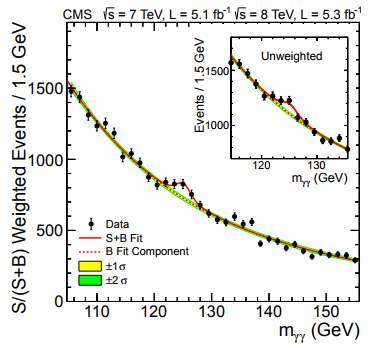
\includegraphics[width=0.49\textwidth]{INT/higgs1.png}}
	\hfill
	\subfloat[Distribution de la masse invariante pour l'analyse $ZZ\rightarrow4l$. Les points représentent les données, les histogrammes pleins le bruit de fond et l'histogramme creux montre le signal attendu pour un boson de \bsc{Higgs} de masse $M_{H}=\SI{125}{\giga\eV}$ ajouté au bruit de fond attendu.]{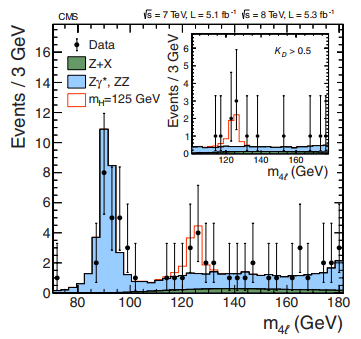
\includegraphics[width=0.49\textwidth]{INT/higgs2.png}}
	\caption{Les deux canaux de désintégration du boson de \bsc{Higgs} ayant permis sa découverte dans l'expérience CMS.}
	\label{higgs}
	\vspace*{-0.3cm}
\end{figure}

Cependant, aucune trace de nouvelle physique n'a été trouvée. Afin d'améliorer la capacité de détection d'une nouvelle physique, le LHC va subir une mise à niveau en \num{2026} afin d'augmenter sa luminosité instantanée par un facteur \num{5} à \num{7.5} et sera renommé pour l'occasion \textit{High Luminosity Large Hadron Collider} (HL-LHC). L'augmentation de la luminosité du LHC aura des conséquences importantes pour les détecteurs placés sur sa ligne de faisceaux (augmentation de l'empilement et du flux de particules produites lors des collisions etc.). Afin de faire face à l'augmentation du taux de collisions et de profiter de cette augmentation de luminosité instantanée, le détecteur CMS doit être mis à niveau. 

Cette thèse se concentre sur la mise à niveau du trajectographe à muons de CMS et plus particulièrement sur l'instrumentation de zones de ce trajectographe par des Resistive Plate Chambers (RPC) de nouvelle génération capables de supporter les flux de particules parcourant ces zones. 

Le premier chapitre décrit succinctement le contexte historique, théorique et expérimental de la physique des particules et présente également ses lacunes. Ceci nous permettra de comprendre les enjeux et la nécessité de construire des collisionneurs et des détecteurs de plus en plus puissants.

Le second chapitre présente le collisionneur le plus puissant actuellement, le LHC, sa chaine d'accélération nécessaire afin d'accélérer les particules et les porter à une énergie inégalée, les différentes expériences placées sur sa ligne de faisceaux et le projet de sa mise à niveau vers le HL-LHC.

Le troisième chapitre décrit de manière détaillée le détecteur CMS ainsi que l'ensemble de ses sous-détecteurs. Il présente également le système de déclenchement et d'acquisition de données ainsi que plusieurs des améliorations nécessaires pour sa mise à niveau afin de pouvoir profiter au maximum de la hausse de la luminosité instantanée qui sera fournie par le LHC.

Le quatrième chapitre se veut un historique sommaire des RPC ainsi qu'une explication de leur principe et modes de fonctionnement en général. Il décrit également les chambres RPC présentes dans CMS, le mélange de gaz utilisé, leur électronique et la détermination de leur point de fonctionnement. Il présente également les améliorations qui seront apportées lors de la mise à niveau du trajectographe à muons ainsi que le type de chambre et d'électronique privilégié pour cette mise à niveau.

Le cinquième chapitre présente les résultats obtenus lors de divers tests en faisceaux à DESY en Allemagne, au PS, SPS, GIF++ basés au CERN, pour un type de chambre utilisant des verres de basse résistivité développé à l'IPNL en collaboration avec nos collègues chinois de l'Université de Tsinghua. Il présente également les types d'électronique utilisés lors de ces tests en faisceaux, les programmes d'analyse utilisés afin d'obtenir ces résultats ainsi que leur validation par simulation Monte-Carlo. Il démontre également la faisabilité de grandes chambres de type RE1/1 en utilisant des verres de taille maximale \SI{32}{\centi\meter}$\times$\SI{30}{\centi\meter} et ce par deux méthodes différentes de pavage.

Le sixième chapitre présente un prototype de PCB à strips ainsi qu'une électronique à base d'ASIC PETIROC2 permettant d'obtenir la position le long des strips par lecture de ceux-ci des deux côtés. Les tout premiers résultats obtenus avec ce PCB qui ont permis de choisir et de privilégier cette solution pour le TDR concernant la mise à niveau du trajectographe à muons de CMS sont également inclus dans ce chapitre.

Le dernier chapitre fait un résumé des résultats et des démarches effectués lors de cette thèse et expose les prochaines étapes à réaliser afin d'inclure cette électronique au sein du détecteur CMS.

Enfin, précisons pour le lecteur aussi peu enclin que l'auteur de cette thèse à la résolution des énigmes engendrées par l'utilisation de sigles  et d'acronymes qu'un glossaire répertoriant ces "mots" est situé en fin d'ouvrage.



\pagestyle{mystyle}
\chapter{ Le vademecum du Modèle Standard }
\renewcommand\chapterillustration{SM/sm2}
\ThisULCornerWallPaper{1}{\chapterillustration}
\minitoc
\lettrine[lines=4, slope=-0.5em]{D}{ans} ce chapitre, un bref historique de la Physique des particules est donné ainsi qu'un résumé et une description de la théorie la plus aboutie dans ce domaine, appelée le Modèle Standard (MS). Il sera également discuté des faiblesses et limites de cette théorie ainsi que de ses éventuelles extensions.

\section{Un bref historique}

\marginpar
{
\centering
%\begin{center}
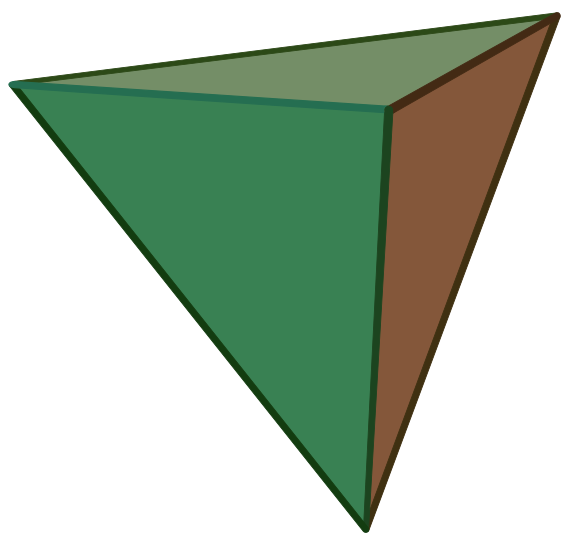
\includegraphics[width=0.25\marginparwidth]{SM/Tetrahedron.png}
\vspace*{-0.25cm}
\begin{center}\normalfont\small {Le Tétraèdre (le Feu).}\end{center}
\vspace*{-0.25cm}
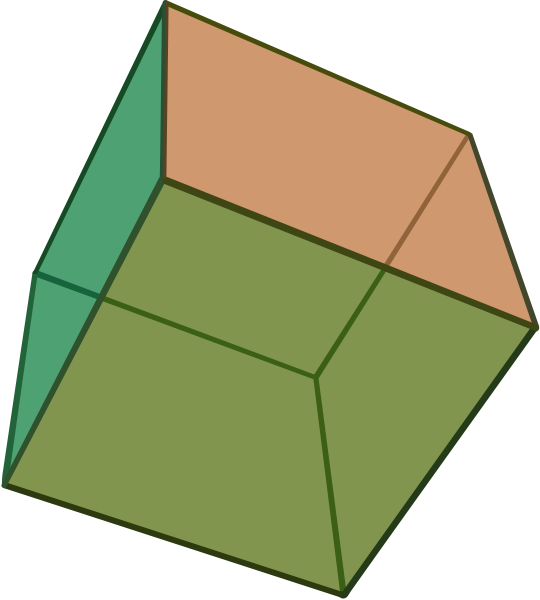
\includegraphics[width=0.25\marginparwidth]{SM/Hexahedron.png}
\vspace*{-0.25cm}
\begin{center}\normalfont\small {Le Cube (la Terre).}\end{center}
\vspace*{-0.25cm}
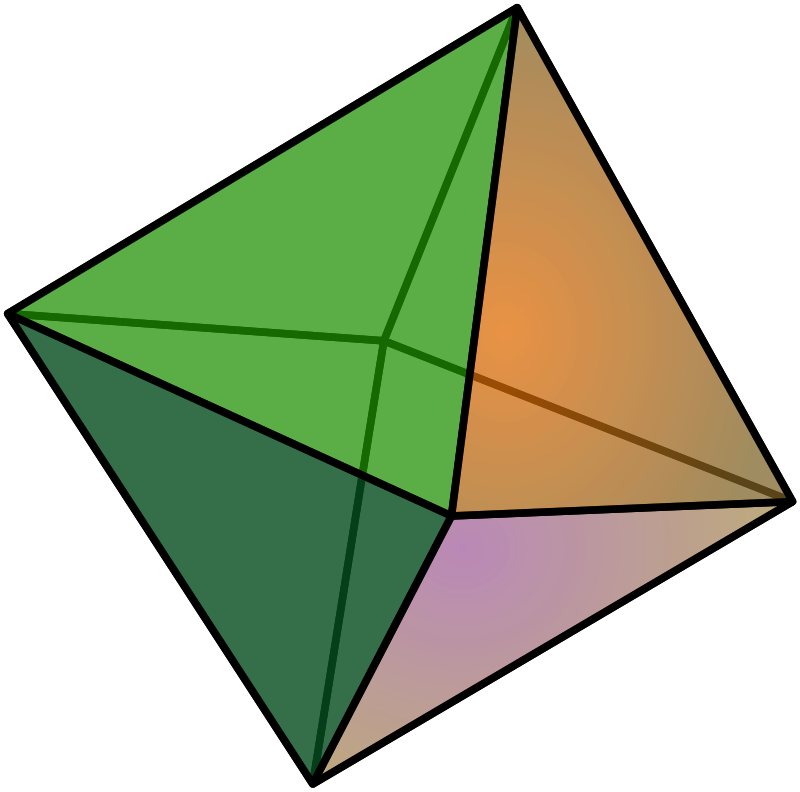
\includegraphics[width=0.25\marginparwidth]{SM/Octahedron.png}
\vspace*{-0.25cm}
\begin{center}\normalfont\small {L'Octaèdre (l'Air).}\end{center}
\vspace*{-0.25cm}
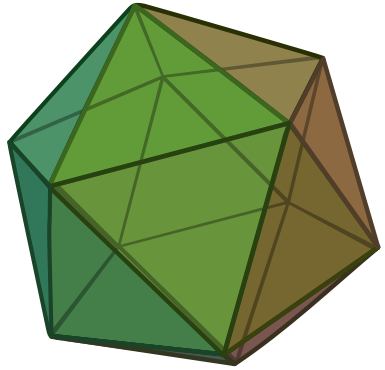
\includegraphics[width=0.25\marginparwidth]{SM/Icosahedron.png}
\vspace*{-0.25cm}
\begin{center}\normalfont\small {L'Icosaèdre (l'Eau).}\end{center}
\vspace*{-0.25cm}
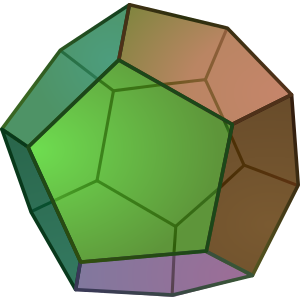
\includegraphics[width=0.25\marginparwidth]{SM/Dodecahedron.png}
\vspace*{-0.25cm}
\begin{center}\normalfont\small {Le Dodécaèdre (l'Univers).}\end{center}
\vspace*{-0.25cm}
\captionof{figure}{Les solides de Platon.}
\label{solides}
%\end{center}
}
De tout temps les hommes ont voulu comprendre et maitriser la nature. Cette quête a amené de nombreux penseurs, et notamment les philosophes Grecs, à proposer des explications sur le monde qui nous entoure, et certaines de leurs idées se révéleront florisantes et donneront naissance des siècles plus tard à la Physique en tant que science au sens moderne du mot. 

Anaxagore (~500-428 av. J.C.) pronait que toute chose est formée de particules élémentaires. Cette idée sera reprise par Empédocle (~495-~435 av J.C) qui proposa, l'eau, la terre, l'air et le feu comme étant ces particules. Platon (428/427 - 348/347 av. J.C.) associera ces quatres éléménts aux polygones réguliers convexes de l'espace à trois dimension (le tétraèdre pour le Feu, le cube pour la Terre, l'octaèdre pour l'Air, l'icosaèdre pour l'Eau, le dodécaère reprèsente l'éther, élément constituant l'Univers (fig.\ref{solides})). On doit à Leucippe (~460-~370 av J.C.) et son disciple Démocrite (~460-~370 av J.C.) le concept d'atomes qui composent la matière et sont indivisibles et séparés par du vide. La véracité de l'atomisme fera débat pendant des siècles et ne sera validé expérimentalement qu'au cours du XIX\ieme siècle.

 Parmis les travaux les plus importants qui prouverons l'existence des atomes, citons ceux de Lavoisier (1743-1794) qui décompose de nombreuses substances en "Éléments". De nombreux travaux sur les gaz, la cristallographie, la physique statistique et la thermodynamique : Bernoulli (1700-1782) : cinétique des gaz, Haüy (1743-1822) : La forme des cristaux reflète la symétrie des "briques élémentaires" le constituant , Dalton (1766-1844) : symbolisation des corps simples et des corps composés par des symboles auxquels il donne un poids de matière (fig.\ref{atom}), et liste des masses atomiques d'un certain nombre d'éléments rapportés à la masse de l'hydrogène, Gay-Lussac (1778-1850) : les rapports des volumes des réactifs et des produits de réaction sont des nombres entiers petits , Maxwell(1831-1879) : dispersion statistique des vitesses des molécules, Boltzmann (1844-1906) : répartition statistique des vitesses dans un gaz , Mendeleïev : Classification périodique des éléments et prédiction de nouveaux atomes (fig.\ref{periodique}). Ces travaux feront passer petit à petit cette théorie en réalité scientifique. 
 
\marginpar
{
	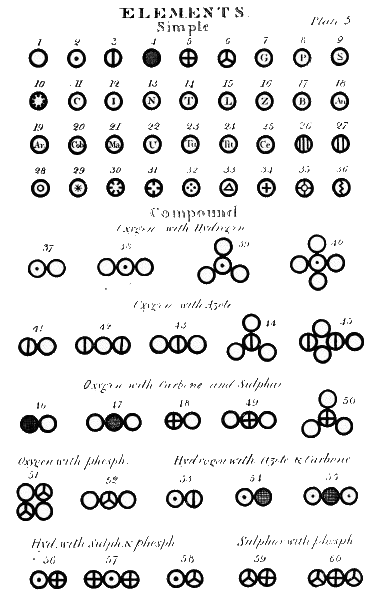
\includegraphics[width=\marginparwidth]{SM/Dalton.png}
    \captionof{figure}{Dessins de divers atomes et molécules tirés de l'ouvrage \textit{A New System of Chemical Philosophy}}
    	\label{atom}
}

\marginpar
{
	\vspace{2cm}
		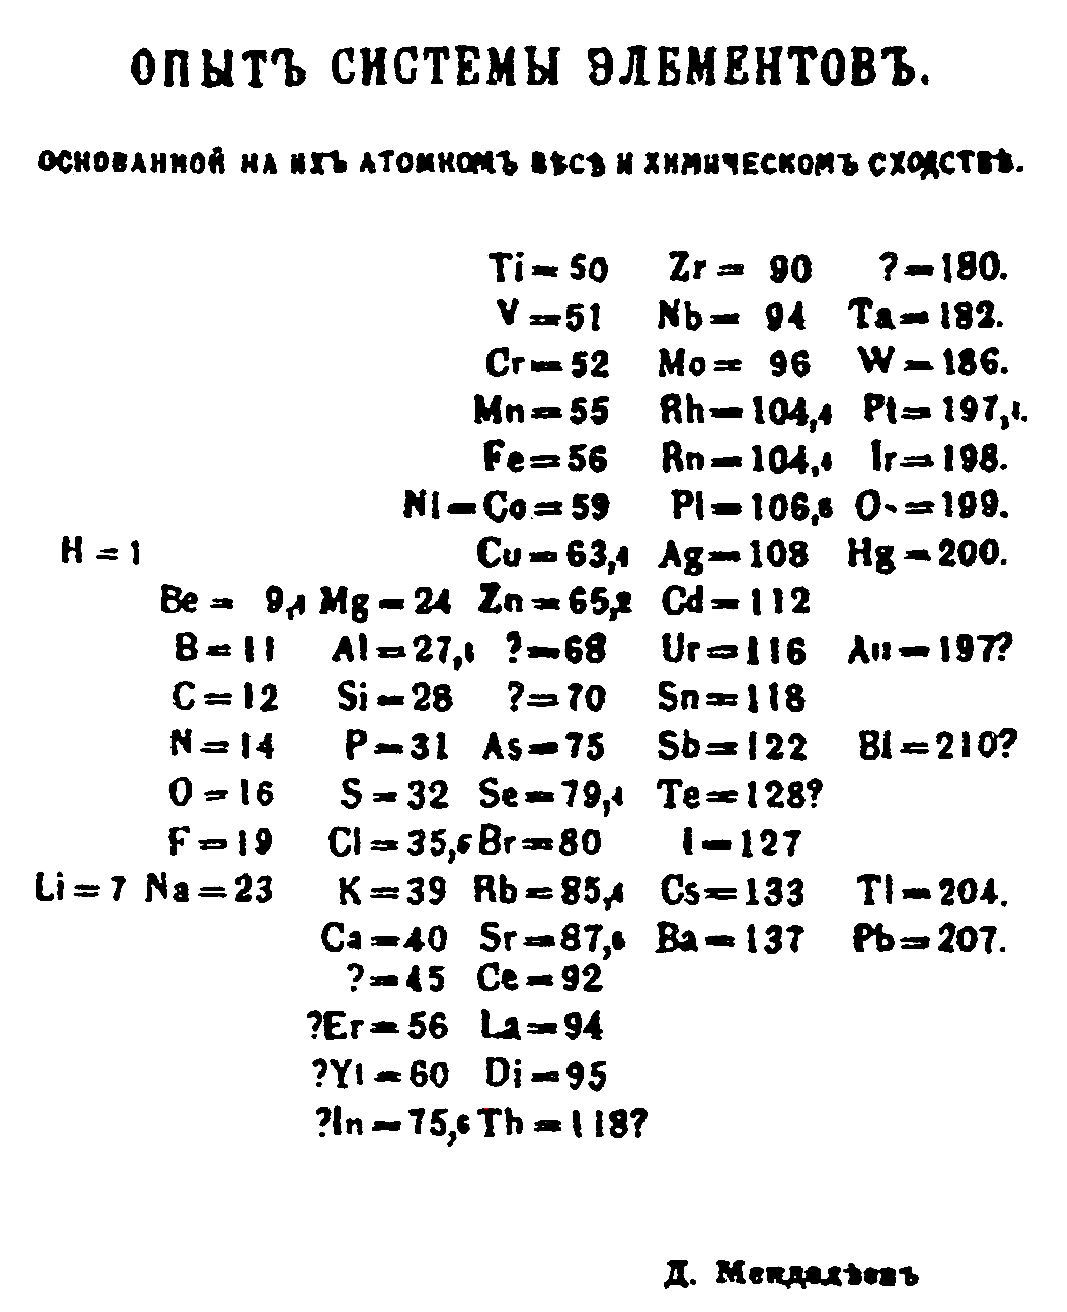
\includegraphics[width=\marginparwidth]{SM/periodique.png}
    \captionof{figure}{Tableau périodique de Mendeleïev}
    	\label{periodique}
}
D'autres domaine de la Physique connaitront des bouleversements importants au cours des siècles : 

Pour la Mécanique et la cosmologie : Copernic (1473-1543) et Galilée (1564-1642) : Modèle héliocentrique, Tycho Brahe (1546-1601) : remise en cause de  l'immuabilité du monde supra-lunaire énoncée par Aristote, Kepler (1571-1630) : Orbite elliptique des planètes, Newton (1643-1727) : théorie de la gravitation universelle, Lagrange (1736-1813) et Hamilton (1805-1865) : Principe de moindre action, Lagrangien, Hamiltonien.

Pour l'électromagnétisme : Coulomb(1736-1806) : loi de Coulomb, Volta(1745-1827): pile voltaïque, Ørsted (1777-1851), Ampère(1775-1836), Faraday(1792-1867), Henry (1797-1878) : les phénomènes d'induction, Maxwell : Équations de Maxwell.

Avec la découverte de l'électron par Thomson (1856-1940) en 1887 qui fût prédit en 1874 par Laming et Stoney. Thomson développe le premier modèle de l'atome, qui est décrit comme une boule de charge nulle possédant un noyau positif avec des électrons négatifs (modèle du "plum-pudding"). On découvre également durant cette période la radioactivité (Becquerel (1852-1908)). La physique semble à cette époque complète et cohérente. Lord Kelvin dira même dans son discours à la "Royal Institution of Great Britain" : \textit{"The beauty and clearness of the dynamical theory, which asserts heat and light to be modes of motion, is at present obscured by two clouds."}. Ces deux "nuages", l'incapacité à détecter l'éther luminifère  (expérience de Michelson-Morley) et la catastrophe ultraviolette du corps noir, donneront naissance respectivement à la relativité restreinte et à la mécanique quantique et feront entrer les physiciens dans la Physique Moderne.

Le début du siècle dernier sera une période florissante pour la physique des particules. Planck (1858-1947), afin de résoudre le problème du corps noir, proposera de quantifier les rayonnements : ceux-ci ne peuvent être qu'un multiple d'une constante qui porte son nom ($h$). Einstein ira plus loin et expliquera durant l'\textit{Annus mirabilis} (1905) l'effet photoélectrique en proposant le photon comme quanta de lumière qui agit comme une particule. Il possera également les bases de la relativité restreinte cette même année, réfutant le concept d'éther. De nombreux physiciens vont ensuite poser les bases de la mécanique quantique: Bohr (1885-1962), Compton (1892-1962), De Broglie (1892-1987), Schrödinger (1887-1961), Heisenberg (1901-1976), Dirac (1902-1984), Pauli (1900-1958). Avec les progrès tant théoriques qu'instrumentaux de Physiciens tels  Rutherford (1871-1937), Chadwick (1891-1974), Fermi (1901-1954), qui explorent le monde subatomique, on découvre les deux forces agissant à l'échelle du subatomique (les forces faible et forte) qui s'ajoutent aux deux force connues à l'époque (la force gravitationnelle et la force électromagnétique). Des physiciens tel Schwinger (1918-1994) veulent continuer la réunification des forces déjà avancée par les travaux de Maxwell ( force éléctrique et magnétique). Dans les années 1960, Weinberg (1933) et Salam (1926-1996) et Glashow (1932), réunissent dans une théorie dite électrofaible les forces électromagnétique et faible. Cette théorie prédit trois bosons ($W^{+}$, $W^{-}$ et $Z^{0}$). Leur théorie nécessite un boson supplémentaire, le boson de Higgs, postulé en 1964 par Brout, Englert, Higgs, Haggen Guralnik et Kibble afin de donner une masse aux particules. Cette théorie est la base du Modèle Standard de la physique des particules. La découverte des quarks amène à la création de la Chromodynamique Quantique (QCD) par Politzer (1949), Wilczek (1951), Gross (1941) afin de décrire l'interaction forte. Elle sera ensuite intégrée au Modèle Standard.

À partir de la seconde moitié du XX\ieme siècle, la Physique Subatomique a tâché de valider cette théorie et notamment par la découverte des bosons  $W^{+}$,$W^{-}$ et $Z^{0}$ en 1983, du quarks top $t$ en 1995, du neutrino tauique en 2000 et du boson de Higgs $h$ en 2012. De nombreux efforts sont également mené afin de continuer l'unification des forces entre elles. On sait cependant que le Modèle Standard, bien que jamais mis en défaut, ne peut tout expliquer. Certaines questions restent ouvertes et cette théorie présente même quelques défauts. La technicouleur, des modèles avec des dimensions supplémentaires ou la Supersymétrie sont des théories d'extension du Modèle Standard. Mais aucune n'a pu être encore validée expérimentalement.

\section{Le Modèle Standard de la physique des particules}
 
Au début du siècle dernier, tout tendait à faire croire que le monde était simplement composé d'atomes; eux mêmes constitués d'électron tournant autour d'un noyau composé de protons et neutrons. Tous les atomes connus avait été soigneusement classés dans le tableau périodique de Mendeleiev. Cependant, grâce à l'invention d'accélérateurs de particules linéaires, cyclotrons (fig. \ref{cyclo}) puis synchrotrons et l'observation des rayons cosmiques, les physiciens découvrirent bientôt qu'une pléthore de particules instables pouvaient être créées durant des désintégrations. Les Physiciens tentèrent bientôt de créer et classer ces particules en utilisant des énergies de faisceau de plus en plus grandes. Ce qui amena à la découverte d'une sous structure au sein même des nucléons\footnote{Protons et neutrons.} qui composent le noyau : les quarks (\ref{structure}).
\marginpar
{
	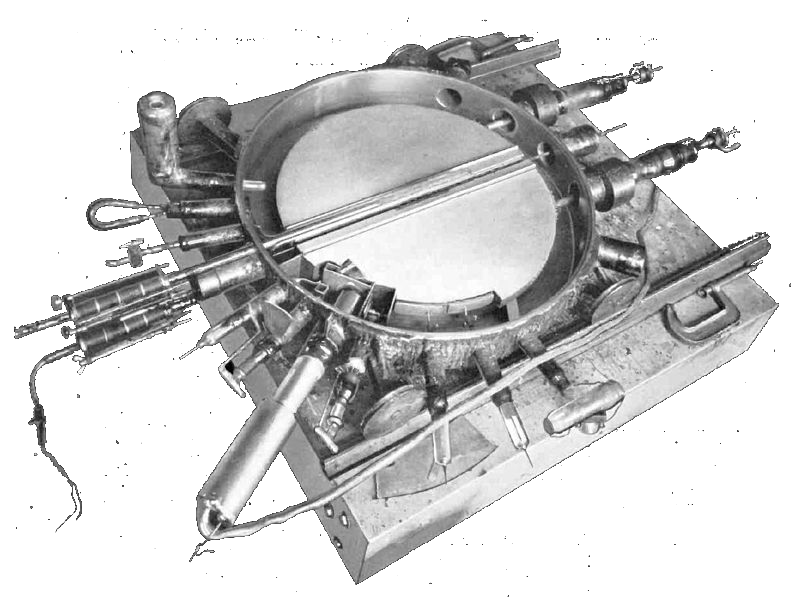
\includegraphics[width=\marginparwidth]{SM/cyclotron.png}
    \captionof{figure}{cyclotron de 27 pouces, accélérateur de $^{2}$H à 4 Mev (Université de Berkley, 1932).}
    	\label{cyclo}
}

\vspace*{-0.5cm}
\begin{figure}[h!]
\centering
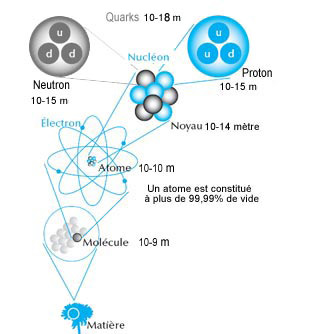
\includegraphics[width=0.50\textwidth]{SM/structure.jpg}
\captionof{figure}{Structure de la matière à différentes échelles.}
\label{structure}
\end{figure}

\vspace*{-0.5cm}
Parallèlement, de nouvelles interactions furent découvertes. Elles expliquaient les désintégrations radioactives ainsi que la cohésion des protons et des neutrons au sein du noyau atomique.

La physique des particules peut se résumer à la combinaison des deux démarches précédentes, à savoir, trouver les particules élémentaires ainsi que trouver les interactions fondamentales que ces particules peuvent subir. La manière dont ces particules interagissent aux moyens de ces interactions est donnée par la formulation mathématique d'une théorie, le Modèle Standard.

\subsection{Les particules élémentaires}
Les particules élémentaires du Modèle Standard, supposées indivisibles\footnote{à ce jour}, peuvent être classées en deux catégories selon leur spin (une propriété quantique intrinsèque à chaque particule) :
\begin{itemize}[label=$\bullet$]
\item les \textit{fermions}, ils constituent la matière et sont de spin demi-entier.
\item les \textit{bosons}, ils sont les messagers de l'interaction et sont de spin entier.
\end{itemize}
Chaque particule du Modèle Standard possède des nombres quantiques telles que sa masse, sa charge électrique, en fraction de l'opposé de la charge électrique de l'électron e par convention (e=$1.6\times10^{-19}$ C). Dans le cadre de la théorie, à chaque particule correspond une anti-particule\footnote{Une particule peut être sa propre anti-particule.} qui possède la même masse mais dont les nombres quantiques sont opposés.

\subsubsection{Les fermions}
Les fermions peuvent être classés en deux catégories selon qu'ils sont sensibles à l'interaction forte ou non. Dans le premier cas, ils font partis des \textit{quarks}, sinon ce sont des \textit{leptons}. Ces deux catégories sont elles-mêmes divisées en trois \textit{générations} (tab. \ref{fermions}).

Les leptons ont une charge électrique entière ($\pm$ 1) pour les électrons, muons et tau, et une charge nulle pour les neutrinos électroniques, neutrinos muoniques et neutrinos tauiques.

Les quarks ont une charge électrique fractionnaire. On associe à chaque quark un nombre quantique appelé "couleur" (Rouge, Vert et Bleu). Dû à la propriété de confinement de couleur, un quark ne peut être isolé et doit se combiner avec un ou deux autre quarks afin de former des \textit{mésons} (fig.\ref{mésons}) et des \textit{baryons} (fig.\ref{baryons}) respectivement. La somme des deux (trois) couleurs des quarks doit constituer un méson (baryon) "blanc" \footnote{Selon l'analogie avec la synthèse additive des couleurs.}. Les mésons et baryons sont regroupés sous le terme générique de \textit{hadrons}.

\marginpar
{
\centering
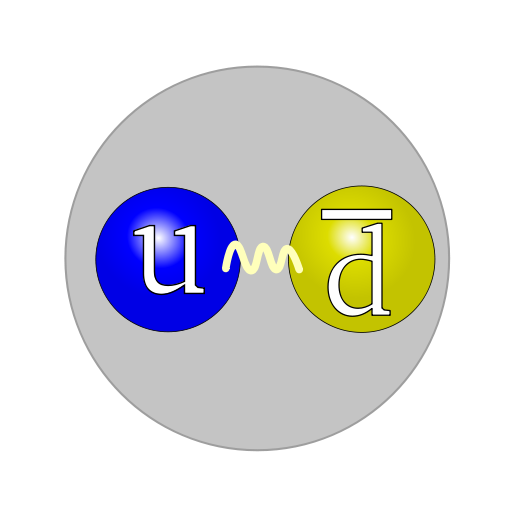
\includegraphics[width=\marginparwidth]{SM/quarks2.png}
\captionof{figure}{Un méson ($\pi^{+}$).}
\label{mésons}
}

\marginpar
{
	\centering
    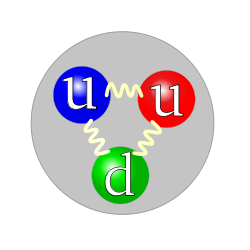
\includegraphics[width=\marginparwidth]{SM/quarks.png}
    \captionof{figure}{Un baryon ($p$).}
    	\label{baryons}
}
	
\marginpar
{
\centering
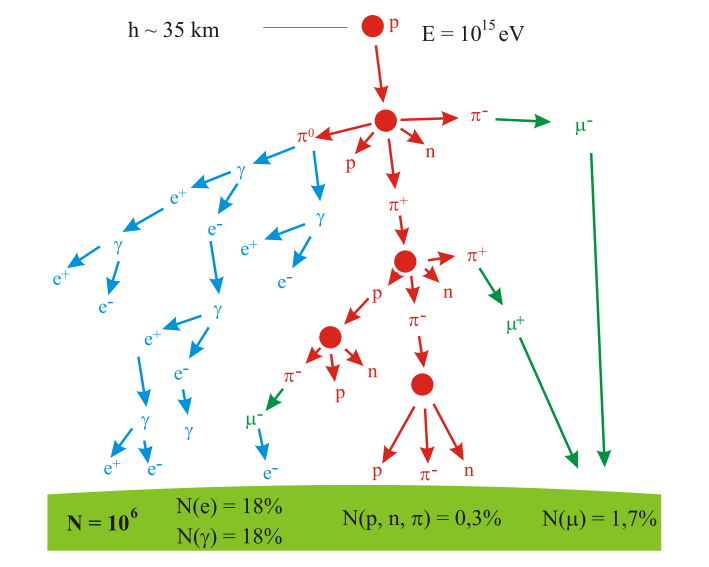
\includegraphics[width=0.95\marginparwidth]{SM/shower.png}
\captionof{figure}{Schéma d'une gerbe atmosphèrique.}
\label{gerbe}
}

La matière qui nous entoure n'est composée que de particules de la première génération. Tous les atomes sont composés d'électrons et de quarks $u$ et $d$ qui s'assemblent pour donner des protons $p$ et neutrons $n$. Les autres particules peuvent être créées si l'énergie disponible est suffisante (lors de gerbe atmosphérique où un proton vient interagir avec des particules de notre atmosphère par exemple \ref{gerbe} ou dans un collisionneur).
\definecolor{Orange}{HTML}{FFDD00}
\definecolor{Orange2}{HTML}{FFC000}
\definecolor{Green}{HTML}{8FB73E}
\definecolor{Green2}{HTML}{4EA700}
\definecolor{Red}{HTML}{EF4123}
\definecolor{Red2}{HTML}{EF2300}
\vspace*{1cm}
\begin{table}[H]
\centering
\begin{tabular}{|O|O|O|O|N}
\hline 
\rowcolor{Orange2}Quarks & 1\iere génération & 2\ieme génération & 3\ieme génération \\
\hline 
\cellcolor{Orange2} Nom &\cellcolor{Orange} Up & \cellcolor{Orange} Charm &  \cellcolor{Orange} Top \\
\cellcolor{Orange2} Notation &\cellcolor{Orange} $u$,$\bar{u}$ & \cellcolor{Orange} $c$,$\bar{c}$ &  \cellcolor{Orange} $t$,$\bar{t}$ \\
\cellcolor{Orange2} Charge &\cellcolor{Orange} $\pm \frac{2}{3}$ & \cellcolor{Orange} $\pm \frac{2}{3}$ &  \cellcolor{Orange} $\pm \frac{2}{3}$ \\
\cellcolor{Orange2} Masse &\cellcolor{Orange} $0.005$ GeV/c$^2$ & \cellcolor{Orange} $1.35$ GeV/c$^2$ &  \cellcolor{Orange} $172.6$ GeV/c$^2$ \\
\hline 
\cellcolor{Orange2} Nom &\cellcolor{Orange} Down & \cellcolor{Orange} Strange &  \cellcolor{Orange} Bottom \\
\cellcolor{Orange2} Notation &\cellcolor{Orange} $d$,$\bar{d}$ & \cellcolor{Orange} $s$,$\bar{s}$ &  \cellcolor{Orange} $b$,$\bar{b}$ \\
\cellcolor{Orange2} Charge &\cellcolor{Orange} $\mp \frac{1}{3}$ & \cellcolor{Orange} $\mp \frac{1}{3}$ &  \cellcolor{Orange} $\mp \frac{1}{3}$ \\
\cellcolor{Orange2} Masse &\cellcolor{Orange} $0.01$ GeV/c$^2$ & \cellcolor{Orange} $0.1$ GeV/c$^2$ &  \cellcolor{Orange} $1.3$ GeV/c$^2$ \\
\hline 
\rowcolor{Green2} Leptons & 1\iere génération & 2\ieme génération & 3\ieme génération \\
\hline
\cellcolor{Green2} Nom & \cellcolor{Green} Électron & \cellcolor{Green} Muon & \cellcolor{Green} Tau \\
\cellcolor{Green2} Notation & \cellcolor{Green} $e^{\pm}$ & \cellcolor{Green} $\mu^{\pm}$ & \cellcolor{Green} $\tau^{\pm}$ \\
\cellcolor{Green2} Charge & \cellcolor{Green} $\pm 1$ & \cellcolor{Green} $\pm 1$ & \cellcolor{Green} $\pm 1$ \\
\cellcolor{Green2} Masse & \cellcolor{Green} $0.511$ MeV/c$^2$ & \cellcolor{Green} $105.7$ MeV/c$^2$ & \cellcolor{Green} $1777$ MeV/c$^2$ \\
\hline 
\cellcolor{Green2} Nom & \cellcolor{Green} Neutrino électronique & \cellcolor{Green} Neutrino muonique & \cellcolor{Green} Neutrino tauique \\
\cellcolor{Green2} Notation & \cellcolor{Green} $\nu_{e}$ & \cellcolor{Green} $\nu_{\mu}$ & \cellcolor{Green} $\nu_{\tau}$ \\
\cellcolor{Green2} Charge & \cellcolor{Green} $0$ & \cellcolor{Green} $0$ & \cellcolor{Green} $0$ \\
\cellcolor{Green2} Masse & \cellcolor{Green} $<0.017$ MeV/c$^2$ & \cellcolor{Green} $<0.27$ MeV/c$^2$ MeV/c$^2$ & \cellcolor{Green} $<35$ MeV/c$^2$ \\

\hline
\end{tabular} 
\captionof{table}{Fermions: Quarks et Leptons.}
\label{fermions}
\end{table}	

\subsubsection{Les bosons}
La description perturbative du Modèle Standard utilise l'échange de bosons virtuelles, afin de décrire l'interaction entre deux particules. Les bosons sont les médiateurs des interactions. Les particules de matière (fermions) interagissent donc entre elles par l'échange de particules de spin 1 correspondant à la force responsable de leur interaction.
\smallskip
Chacune des quatre interactions possède donc un ou plusieurs bosons appelés bosons de jauge (bosons vecteurs) (Tab.\ref{bosons}) :

\marginpar
{
\begin{center}
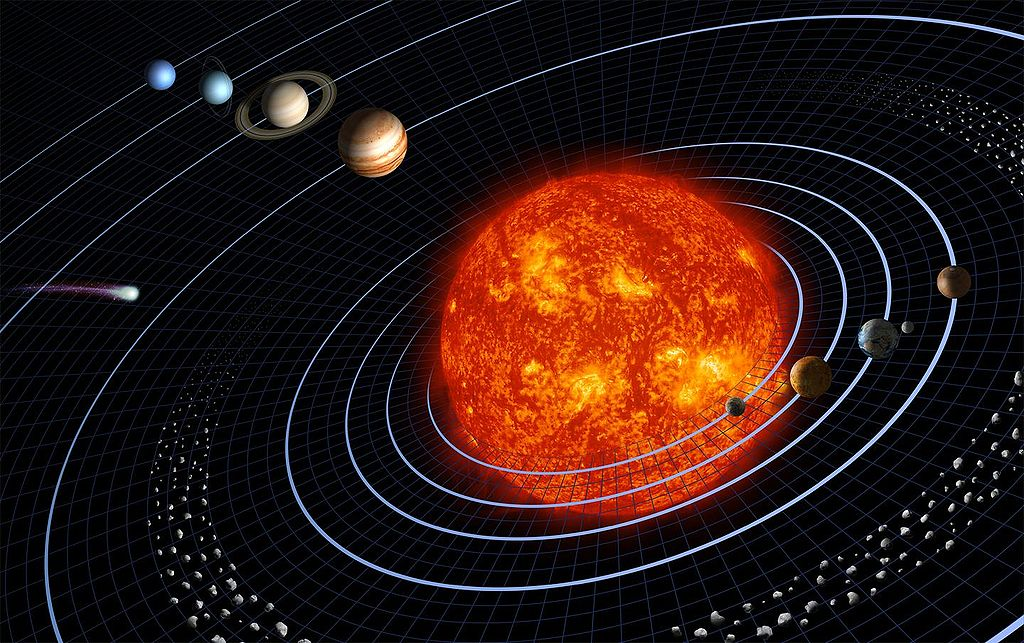
\includegraphics[width=\marginparwidth]{SM/solaire.jpg}
\begin{center}\normalfont\small {(a) Gravité : Système solaire.}\end{center}
\end{center}
}

\marginpar
{
\centering
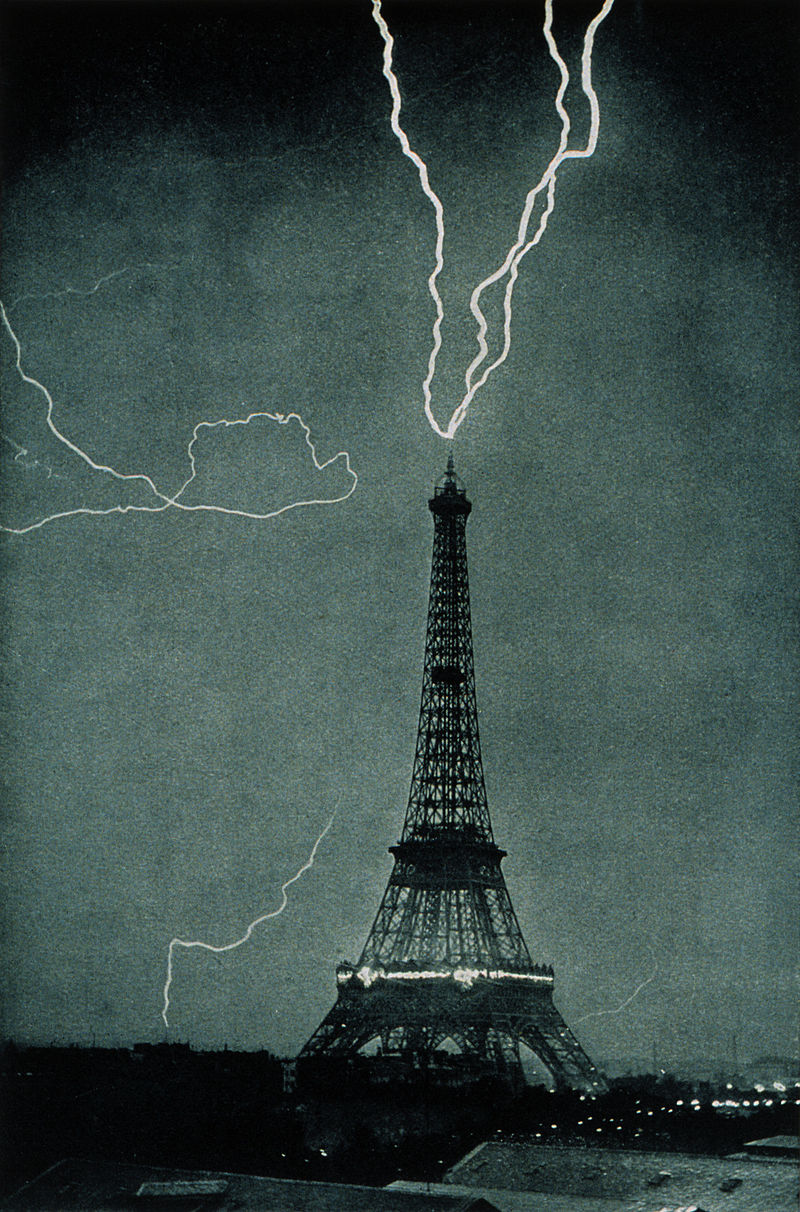
\includegraphics[width=\marginparwidth]{SM/foudre.jpg}
\begin{center}\normalfont\small {(b) Électromagnétisme : la foudre.}\end{center}
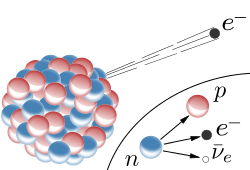
\includegraphics[width=\marginparwidth]{SM/beta.png}
\begin{center}\normalfont\small {(c) Interaction faible : désintégration $\beta$.}\end{center}
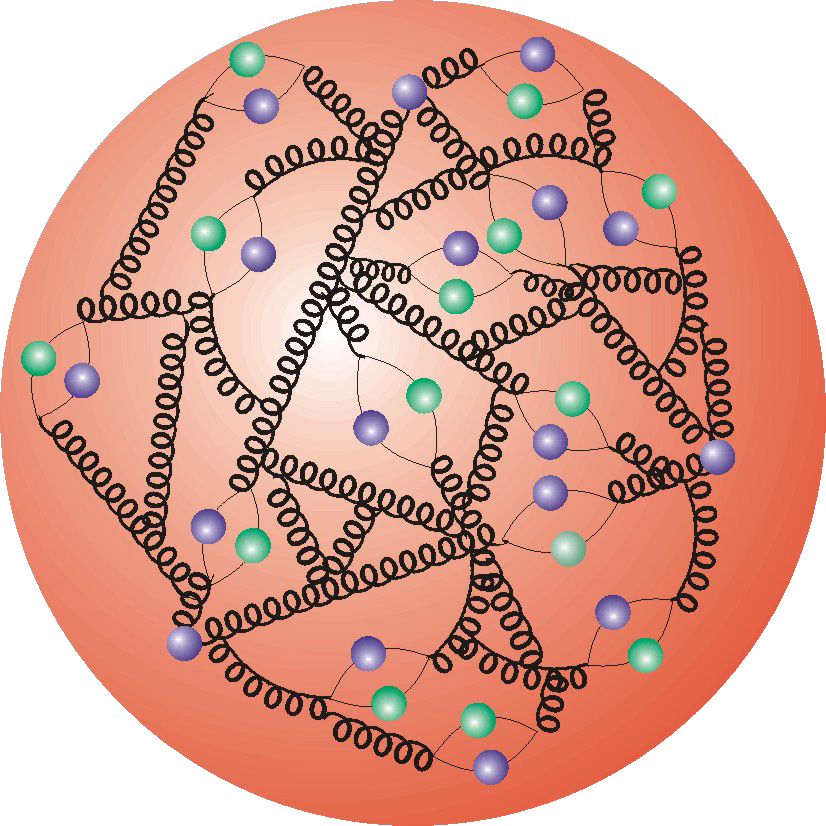
\includegraphics[width=0.8\marginparwidth]{SM/quarks3.png}
\begin{center}\normalfont\small {(d) Interaction forte : confinement.}\end{center}
\captionof{figure}{Exemple d'effets des 4 interactions.}
}

\begin{itemize}[label=$\bullet$]
\item \textbf{L'interaction gravitationnelle} est la première à avoir été découverte et expliquée (Galilée, Newton). Elle est négligeable à l'échelle atomique. Elle est gouvernée par la masse des corps mise en jeu et elle domine à grande échelle ( Univers, Galaxies, Planètes), son rayon d'action est infini. Sa description quantique repose sur un boson de spin 2 qui est encore activement recherché. Un pas décisif à été fait grâce à la détection par les expériences Virgo et Ligo des ondes Gravitationnelle. Cette interaction est la seule à ne pas être intégrée au Modèle Standard. Elle est actuellement décrite par la Relativité Générale qui est une approche non quantique.

\item \textbf{L'interaction électromagnétique} gouverne les interactions entre les particules chargées. C'est l'une des interactions qui nous est la plus familière car elle est prépondérante dans notre vie quotidienne ( lumière, chimie, frottements ...). Tout comme la gravité, son rayon d'action est infini. Son boson médiateur est le photon $\gamma$.

\item \textbf{L'interaction faible} à été découverte et comprise à travers la désintégration de particules avec changements de saveurs. Elle fait passer d'un fermion à un autre (par exemple lors de la désintégration $\beta$, elle transforme un neutron en un proton en changeant un quark $d$ en un quark $u$ avec la création d'un neutrino et d'un électron). Les bosons médiateurs de l'interaction sont les bosons $W^{+}$ $W^{-}$ $Z^{0}$. Sa portée est de l'ordre de 10$^{-18}$ m due à la masse des bosons médiateur.

\item \textbf{L'interaction forte} permet l'échange de couleur entre les quarks et la création et l'annihilation de particules. Elle est responsable de la cohésion du noyau, et elle lie les nucléons entre eux à l'intérieur du noyau atomique. Ses bosons médiateur sont les gluons et sont au nombre de huit. Bien que les gluons soient supposés de masse nulle, la portée de l'interaction est de l'ordre de 10$^{-15}$ m. Cette portée est la conséquence du principe de confinement de couleur qui affecte les quarks. En effet, cette interaction a la propriété de voir son intensité augmenter avec la distance, ce qui à tendance à regrouper les quarks entre eux. Cette propriété est également responsable du processus d'hadronisation des quarks et de la création de jets.
\end{itemize}

\vspace{1cm}
\begin{table}[h!]
\centering
\begin{tabular}{|O|O|O|O|N}
\hline 
\rowcolor{Red2}Interaction&Rayon d'action&Bosons de jauge&Masses\\
\hline 
\cellcolor{Red}\shortstack{ Forte }&
\cellcolor{Red}\shortstack{ $2.5\times10^{-15}$ m}& 
\cellcolor{Red}\shortstack{  Gluons (8)}&
\cellcolor{Red}\shortstack{ 0}\\
\hline 
\cellcolor{Red}\shortstack{ Electromagnétique }&
\cellcolor{Red}\shortstack{ $\infty$}& 
\cellcolor{Red}\shortstack{Photon $\gamma$}&
\cellcolor{Red}\shortstack{0}\\
\hline 
\cellcolor{Red}\shortstack{Faible}&
\cellcolor{Red}\shortstack{$10^{-18}$ m }& 
\cellcolor{Red}\shortstack{$W^{\pm}$,$Z^{0}$}&
\cellcolor{Red}\shortstack{$80.399$,$91.188$ Gev/c$^{2}$}\\
\hline 
\cellcolor{Red}\shortstack{Gravitationnelle}&
\cellcolor{Red}\shortstack{$\infty$}& 
\cellcolor{Red}\shortstack{(Graviton)}&
\cellcolor{Red}\shortstack{(inconnue)}\\
\hline 
\end{tabular} 
\captionof{table}{Bosons : Interactions.}
\label{bosons}
\end{table}

\subsubsection{Le boson de Higgs}
Le boson de Higgs ($H^{0}$) est nécessaire afin de donner la masse des bosons $W^{\pm}$, $Z^{0}$ et des fermions. Bien que postulé en 1964, il n'a été découvert qu'en 2012 par les expériences CMS et ATLAS en 2012. Contrairement au bosons vecteur, le boson de Higgs est de spin 0.
\newpage
Toutes ces particules peuvent être résumer dans le tableau suivant : 

\begin{minipagewithmarginpars}[h]{\textwidth}
\vspace{-0.5cm}
\centering
\hspace*{-1.5cm}
\includestandalone{./SM/bestiaire}
\captionof{figure}{Classification des quarks, leptons et bosons.}
\label{bestiaire}
\marginpar
{
\vspace*{1.5cm}
%\begin{center}
\centering
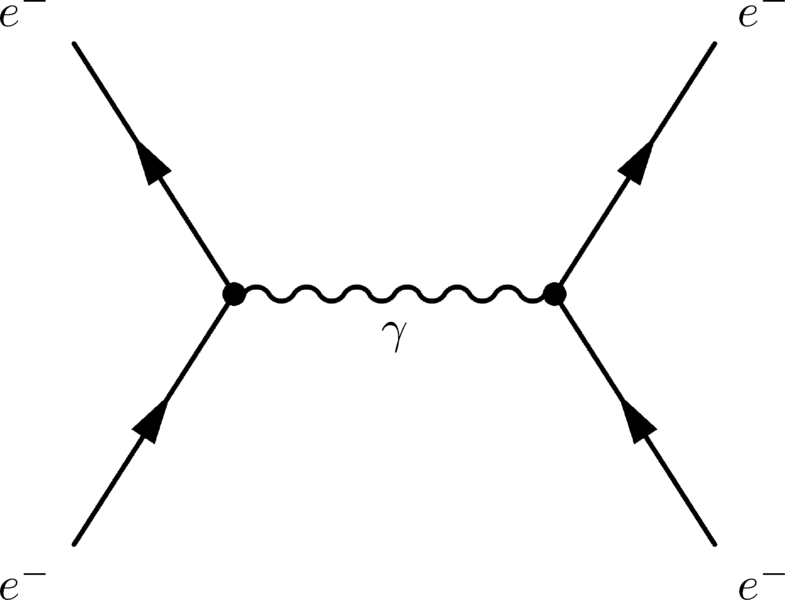
\includegraphics[width=\marginparwidth]{SM/feyn0.png}
\begin{center}\normalfont\small {(a) Développement à l'arbre.}\end{center}
%\end{center}
}
\end{minipagewithmarginpars}
\subsection{Le formalisme du Modèle Standard}
\marginpar
{
\centering
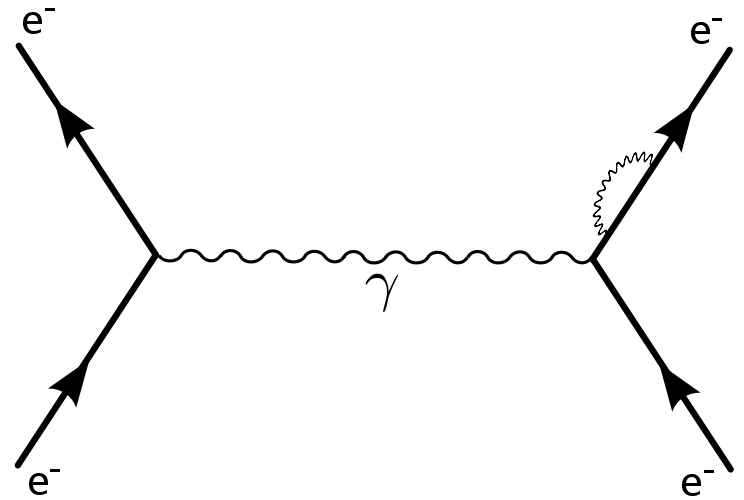
\includegraphics[width=\marginparwidth]{SM/feyn1.png}
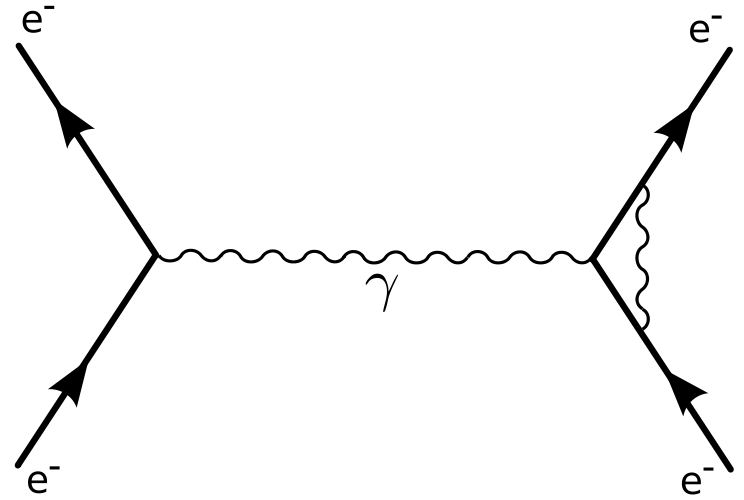
\includegraphics[width=\marginparwidth]{SM/feyn2.png}
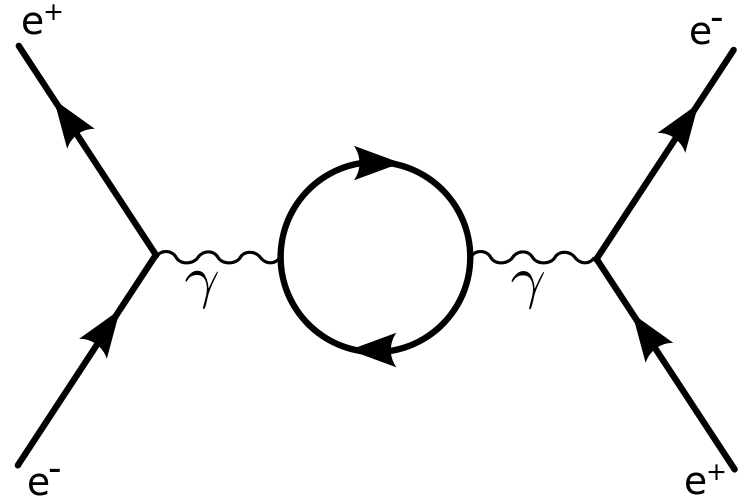
\includegraphics[width=\marginparwidth]{SM/feyn3.png}
\begin{center}\normalfont\small {(b) Développement à l'ordre 1.}\end{center}
\captionof{figure}{Exemple de diagrammes de Feynman pour le développement en série de la diffusion électron-électron.}
\label{feyn}
}
Le Modèle Standard est une théorie non-abélienne où les interactions sont régis par des symétries locales de jauge. Elle repose sur la théorie quantique des champs qui permet de décrire les particules et leurs interactions. Cette théorie est à la fois quantique et relativiste. Elle permet donc de caractériser les interactions par des probabilités de transition d'un état initial à un état final, ainsi que de rendre compte du temps de propagation des interactions, la description des particules à hautes énergie et les créations annihilation de particules.

Dans cette théorie, à chaque type de particule est associé un champ $\psi(\vec{x},t)$ et les interactions sont liées à des propagateurs. La création (l'annihilation) de particules est associé à des opérateurs qui excitent(désexciter) le champ de particules à une position $\vec{x}$ et à un temps $t$. L'un des postulat de la théorie quantique des champs est que l'ensemble des informations de la théorie est contenu dans un Lagrangien $\mathcal{L}$ qui s'exprime en fonction des champs et de leurs dérivées. Il est possible, à partir de ce Lagrangien d'obtenir les équations de mouvements en minimisant sont action $S=\int\mathcal{L}\Diff4{x}$.
Le Modèle Standard et une théorie perturbative, c'est à dire que les observables sont calculées par une méthode qui s'appuie sur un développement en série dont la précision augmente avec l'ordre. Au premier ordre, l'observable est dite être calculé à l'arbre ou LO (Leading Order). Ce développement en série n'est valable que si les constantes de couplage des interactions reste faible devant l'unité. Ce développement en série peut être schématisé grâce aux diagrammes de Feynmann (fig. \ref{feyn}), qui sont des diagramme représentant des règles de calculs. Chaque types de particules et d'interactions posséde son symbole et à chaque particules doit être connécté par un vertex (représentant une interactions).

Le principe selon lequel les interactions sont gouvernés par des symétries est également un postulat des important du Modèle Standard. De par le théorème de Noether, les symétries continues sont liées à des quantités physique qui se conserve. Le Modèle Standard est basé sur le produit direct du groupe de la chromodynamique quantique, décrivant l'interaction forte, qui impose une conservation de la charge de couleur, $SU(3)_{C}$ et du groupe de la théorie électrofaible, $SU(2)_{L} \otimes U(1)_{Y}$, imposant une symétrie locale de l'isospin $I$ associé au groupe $SU(2)_{L}$ et une symètrie locale de l'hypercharge $Y$ du groupe $U(1)_{Y}$.

\subsection{Lagrangien du modèle standard}
Le modèle standard est une théorie de Jauge qui se base sur le groupe $SU(3)_{C} \otimes SU(2)_{L} \otimes U(1)_{Y}$ dont le lagrangien peut s'écrire sous la forme :

\begin{equation}
\mathcal{L_{MS}}=\mathcal{L}_{\mathrm{Yang-Mills}}+\mathcal{L}_{\mathrm{Dirac}}+\mathcal{L}_{\mathrm{Yukawa}}+\mathcal{L}_{\mathrm{Higgs}}
\end{equation}

\subsubsection{Le terme de Yang-Mills (secteur de jauge)}
Le secteur de jauge est la partie cinématique des champs de jauge :
\begin{equation}
\mathcal{L}_{\mathrm{Yang-Mills}}=-\frac{1}{4}B_{\mu\nu}B^{\mu\nu}-\frac{1}{4}W_{\mu\nu}^{a}W_{a}^{\mu\nu}-\frac{1}{4}G_{\mu\nu}^{A}G_{A}^{\mu\nu}
\end{equation}
où 
\begin{equation}
B_{\mu\nu}=\partial_{\mu}B_{\nu}-\partial_{\nu}B_{\mu}
\end{equation}
avec $B_{\mu}$ le champ isoscalaire associé au groupe d'hypercharge $U(1)_{Y}$,
\begin{equation}
W_{\mu\nu}^{a}=\partial_{\mu}W_{\nu}^{a}-\partial_{\nu}W_{\mu}^{a}+g\epsilon_{abc}W_{\mu}^{b}W_{\nu}^{c}
\end{equation}
où $W_{\mu}^{a} (a=1,2,3)$ est le triplet d'isospin I=1 du groupe de l'isospin faible $SU(2)_{L}$, g la constante de couplage de l'isospin faible et $\epsilon_{abc}$ les constantes de structures antisymétriques correspondantes.  
\begin{equation}
G_{\mu\nu}^{A}=\partial_{\mu}G_{\nu}^{A}-\partial_{\nu}G_{\mu}^{A}+g'\epsilon_{ABC}G_{\mu}^{B}G_{\nu}^{C}
\end{equation}
les champs des gluons $G_{\mu}^{A} (A=1,2,..,8)$, bosons vecteurs de $SU(3)_{c}$, $g'$ la constante de couplage de couleur et $f_{ABC}$ les constantes de structures de $SU(3)_{C}$.
La nature non-Abélienne de $SU(2)_{L}$ et $SU(3)_{c}$ amène à des termes supplémentaires dans l'écriture des champs du triplet d'isospin et des champs de gluons. Ce sont ces termes qui sont reponsables de l'interaction des bosons $W$ et des gluons $g$.

\subsubsection{Le secteur de Dirac}
Le secteur de Dirac décrit les interactions des fermions avec les bosons de jauge. Dans le secteur électrofaible, les fermions se regroupent de manière asymétrique dans des doublets d'isospin faible de chiralité gauche et dans des singulets de chiralité droite (tab. \ref{doublets}). Il y a violation maximale de la parité de $SU(2)_{L}\otimes U(1)_{Y}$

\begin{table}[H]
\centering
\begin{tabular}{|L|L|} 
\hline
\multicolumn{2}{|Cc|}{Quarks} \\
\hline
Gauches $Q_{\alpha L}^{i}$ & $\begin{pmatrix} 
u^{i}\\
d^{i}
\end{pmatrix}_{L},\ \begin{pmatrix} 
c^{i}\\
s^{i}
\end{pmatrix}_{L},\ \begin{pmatrix} 
t^{i}\\
b^{i}
\end{pmatrix}_{L}$ \\
\hline
Droits $Q_{\beta R}^{i}$&$ u_{iR},\ d_{iR},\ c_{iR},\ s_{iR},\ t_{iR},\ b_{iR}$\\
\hline
\multicolumn{2}{|Cc|}{Leptons} \\
\hline
Gauche $L_{\alpha L}$& $\begin{pmatrix} 
\nu_{e}\\
e
\end{pmatrix}_{L},\ \begin{pmatrix} 
\nu_{\mu}\\
\mu
\end{pmatrix}_{L},\ \begin{pmatrix} 
\nu_{\tau}\\
\tau
\end{pmatrix}_{L} $\\
\hline
Droits $L_{\gamma R}$& $e_{R},\ \mu_{R},\ \tau_{R},\ \left(\nu_{e R},\ \nu_{\mu R},\ \nu_{\tau R}\right)$ \\
\hline
\end{tabular}
\captionof{table}{Doublets et singulets pour $SU(2)_{L}$ ;$i$=1,2,3 couleurs, $\alpha$=1,2,3 familles, $\beta$={u,d,s,c,t,b}, $\gamma$={$e$,$\mu$,$\tau$,$\left(\nu_{e},\nu_{\mu},\nu_{\tau}\right)$}}.
\label{doublets}
\end{table}	

En suivant ces notations le secteur de Dirac du Lagrangien du Modèle Standard s'écrit:
\marginpar
{
\begin{equation*}
\sigma_{1}=\begin{pmatrix} 
0&1\\
1&0\\
\end{pmatrix}
\end{equation*}
\vspace{0.2cm}
\begin{equation*}
\sigma_{2}=\begin{pmatrix} 
0&-i\\
i&0\\
\end{pmatrix}
\end{equation*}
\vspace{0.2cm}
\begin{equation*}
\sigma_{3}=\begin{pmatrix} 
1&0\\
0&-1\\
\end{pmatrix}
\end{equation*}
\captionof{figure}{Les matrices canoniques de Pauli.}
\label{Pauli}
}
\marginpar
{
\begin{equation*}
\lambda_{1}=\begin{pmatrix} 
0&1&0\\
1&0&0\\
0&0&0
\end{pmatrix}
\end{equation*}
\vspace{0.2cm}
\begin{equation*}
\lambda_{2}=\begin{pmatrix} 
0&-i&0\\
i&0&0\\
0&0&0
\end{pmatrix}
\end{equation*}
\vspace{0.2cm}
\begin{equation*}
\lambda_{3}=\begin{pmatrix} 
1&0&0\\
0&-1&0\\
0&0&0
\end{pmatrix}
\end{equation*}
\vspace{0.2cm}
\begin{equation*}
\lambda_{4}=\begin{pmatrix} 
0&0&1\\
0&0&0\\
1&0&0
\end{pmatrix}
\end{equation*}
\vspace{0.2cm}
\begin{equation*}
\lambda_{5}=\begin{pmatrix} 
0&0&-i\\
0&0&0\\
i&0&0
\end{pmatrix}
\end{equation*}
\vspace{0.2cm}
\begin{equation*}
\lambda_{6}=\begin{pmatrix} 
0&0&0\\
0&0&1\\
0&1&0
\end{pmatrix}
\end{equation*}
\vspace{0.2cm}
\begin{equation*}
\lambda_{7}=\begin{pmatrix} 
0&0&0\\
0&0&-i\\
0&i&0
\end{pmatrix}
\end{equation*}
\vspace{0.2cm}
\begin{equation*}
\lambda_{8}=\frac{1}{\sqrt{3}}\begin{pmatrix} 
1&0&0\\
0&1&0\\
0&0&-2
\end{pmatrix}
\end{equation*}
\captionof{figure}{Les matrices canoniques de Gell-Mann.}
\label{Gell-Mann}
}

\begin{equation}
\begin{split}
\mathcal{L}_{\mathrm{Dirac}}=&i\sum_{\alpha=1}^{3}\bar{L}_{\alpha L}\gamma_{\mu}D_{L_{L}}^{\mu}L_{\alpha L}+\sum_{\gamma=1}^{3(6)}\bar{L}_{\gamma R}\gamma_{\mu}D_{L_{R}}^{\mu}L_{\gamma R}\\
&+\sum_{\alpha=1}^{3}\sum_{i=1}^{3}\bar{Q}_{\alpha L}^{i}\gamma_{\mu}D_{Q_{L}}^{\mu}Q_{\alpha L}^{i}+\sum_{\beta=1}^{6}\sum_{i=1}^{3}\bar{Q}_{\beta R}^{i}\gamma_{\mu}D_{Q_{R}}^{\mu}Q_{\beta R}^{i}
\end{split}
\end{equation}
Avec les dérivées covariantes de la forme : 
\begin{equation}
D_{\mu L_{L}}=\partial_{\mu} -ig\frac{\sigma^a}{2}W_{\mu}^{a}-ig'\frac{Y^{W}_{L}}{2}B_{\mu}
\end{equation}
\begin{equation}
D_{\mu L_{R}}=\partial_{\mu} -ig'\frac{Y^{W}_{R}}{2}B_{\mu}
\end{equation}
\begin{equation}
D_{\mu Q_{L}}=\partial_{\mu} -ig\frac{\sigma^a}{2}W_{\mu}^{a}-ig'\frac{Y^{W}_{L}}{2}B_{\mu}-ig''\frac{\lambda^{A}}{2}Q_{\mu}^{A}
\end{equation}
\begin{equation}
D_{\mu Q_{R}}=\partial_{\mu}ig'\frac{Y^{W}_{R}}{2}B_{\mu}-ig''\frac{\lambda^{A}}{2}Q_{\mu}^{A}
\end{equation}
où $\sigma^{a}$ sont les générateur de $SU(2)_{L}$ (matrices de Pauli (Fig. \ref{Pauli})), $\lambda^{A}$ les générateurs de $SU(3)_{c}$ (matrices de Gell-Mann (Fig. \ref{Gell-Mann})) et $Y^{W}$, l'hypercharge faible, le générateur de $U(1)_{Y}$. 
Afin d'obtenir les charges électriques pour chaque fermions, on pose:
\begin{multline}
\begin{split}
&Y^W(L_{\alpha L})=-1,\ &Y^W(e_{R},\mu_{R},\tau_{R})=-2,\ &\left(Y^W(\nu_{e R},\nu_{\mu R},\nu_{\tau R})=0\right)\\
&Y^W(Q_{\alpha L})=\frac{1}{3},\ &Y^W(u_{R},c_{R},t_{R})=\frac{4}{3},\ &Y^W(d_{R},s_{R},b_{R})=-\frac{2}{3}
\end{split}
\end{multline}  

\subsubsection{Le secteur de Higgs} 
La symétrie électrofaible est incompatible avec la description de fermion massif. En effet, dans le Lagrangien les termes de masses des fermions sont de la forme 
\begin{equation}
\mathcal{L_{M}}=-m\bar{\phi}\phi=-m \left(\phi_{L}^{\dagger}\phi_{R}+\phi_{R}^{\dagger}\phi_{L}\right)
\end{equation}
Cependant, ces termes brisent la symétrie $SU(2)$ et n'est donc pas inclus dans le Lagrangien. De plus, l'expérience montre que les bosons de jauge $W$ doivent posséder une masse. Or l'introduction des termes de masses pour ces boson est également impossibles pour les mêmes raisons.

Afin de résoudre ces problèmes, on introduit un champ scalaire complexe $\phi$, doublet de $SU(2)_{L}$ de quatre champs réels $\phi_{i}$ et d'hypercharge $Y=1$ :
\begin{equation}
\phi=\begin{pmatrix} 
\phi^{+}\\
\phi^{0}
\end{pmatrix}=\frac{1}{\sqrt{2}}\begin{pmatrix} 
\phi_{1}+\phi_{2}\\
\phi_{3}+\phi_{4}
\end{pmatrix}
\end{equation}
On utilise l'expression du Lagrangien la plus générale pour un champ scalaire complexe de $SU(2)$:
\begin{equation}
\mathcal{L}_{\mathrm{Higgs}}=\left(D_{\mu}\phi\right)^{\dagger}\left(D^{\mu}\phi\right)-V(\phi),
\end{equation}
avec 
\begin{equation}
D_{\mu}=\partial_{\mu} -ig\frac{\sigma^a}{2}W_{\mu}^{a}-ig'\frac{Y}{2}B_{\mu}.
\end{equation}
Afin que le lagrangien $\mathcal{L}_{\mathrm{Higgs}}$ soit invariant globalement, le potentiel scalaire $V(\phi)$ ne doit pas comporter de puissance impaires de $\phi$. De plus, afin que la théorie reste renormalisable, les puissances au delà de $\phi^4$ sont à proscrire.

Le potentiel $V(\phi)$ est donc de la forme :
\begin{equation}
V(\phi)=\mu^{2}\phi^{\dagger}\phi+\lambda\left(\phi^{\dagger}\phi\right)^2,
\end{equation}
et a un profil différent selon les signes de $\mu^{2}$ et de $\lambda$ (Fig. \ref{profile}).
\marginpar{ 
\resizebox {\marginparwidth} {!} 
{
\begin{tikzpicture}
\begin{axis}[view={15}{15},yticklabels={,,},xticklabels={,,},zticklabels={,,},mesh/interior colormap name=hot,colormap/blackwhite]
\addplot3[surf,shader=faceted,samples=50,fill opacity=0.5,opacity=0.4,domain=0:1.05,y domain=0:2*pi,z buffer=sort]({x * cos(deg(y))}, {x * sin(deg(y))}, {-x*x-x*x*x*x});
\end{axis}
\end{tikzpicture}
}
\begin{center}\normalfont\small {(a) $\mu^{2}<0$ , $\lambda<0$.}\end{center}
\resizebox {\marginparwidth} {!} 
{
\begin{tikzpicture}
\begin{axis}[view={15}{15},yticklabels={,,},xticklabels={,,},zticklabels={,,},mesh/interior colormap name=hot,colormap/blackwhite]
\addplot3[surf,shader=faceted,samples=50,fill opacity=0.5,opacity=0.4,domain=0:1.05,y domain=0:2*pi,z buffer=sort]({x * cos(deg(y))}, {x * sin(deg(y))}, {+x*x+x*x*x*x});
\end{axis}
\end{tikzpicture}
}
\begin{center}\normalfont\small {(b) $\mu^{2}>0$ , $\lambda>0$.}\end{center}
\resizebox {\marginparwidth} {!} 
{
\begin{tikzpicture}
\begin{axis}[view={15}{15},yticklabels={,,},xticklabels={,,},zticklabels={,,},mesh/interior colormap name=hot,colormap/blackwhite]
\addplot3[surf,shader=faceted,samples=50,fill opacity=0.5,opacity=0.4,domain=0:1.05,y domain=0:2*pi,z buffer=sort]({x * cos(deg(y))}, {x * sin(deg(y))}, {+x*x-x*x*x*x});
\end{axis}
\end{tikzpicture}
}
\begin{center}\normalfont\small {(c) $\mu^{2}>0$ , $\lambda<0$.}\end{center}
\resizebox {\marginparwidth} {!} 
{
\begin{tikzpicture}
\begin{axis}[view={15}{15},yticklabels={,,},xticklabels={,,},zticklabels={,,},mesh/interior colormap name=hot,colormap/blackwhite]
\addplot3[surf,shader=faceted,samples=50,fill opacity=0.5,opacity=0.4,domain=0:1.05,y domain=0:2*pi,z buffer=sort]({x *cos(deg(y))},{x*sin(deg(y))},{-x*x+x*x*x*x});
\end{axis}
\end{tikzpicture}
}
\begin{center}\normalfont\small {(d) $\mu^{2}<0$ , $\lambda>0$.}\end{center}
\captionof{figure}{Les différents profils de $V(\phi)$ selon les signes de $\mu^{2}$ et $\lambda$.}
\label{profile}
}
Les cas où $\mu^{2}>0$ ne possède qu'un minimum en $0$, ce qui est inutile. Le cas $\mu^{2}<0$ n'est pas stable. Il ne reste que le cas où $\mu^{2}<0$ et $\lambda>0$.

\begin{minipagewithmarginpars}[h]{0.95\textwidth}
\centering
\begin{tikzpicture}
\begin{axis}[view={7}{7},yticklabels={,,},xticklabels={,,},zticklabels={,,},mesh/interior colormap name=hot,colormap/blackwhite,]
\addplot3[surf,shader=faceted,samples=50,fill opacity=0.5,opacity=0.4,domain=0:1.05,y domain=0:pi,z buffer=sort]({x * cos(deg(y))}, {x * sin(deg(y))}, {-x*x+x*x*x*x});
\addplot3[->] coordinates{(0,0,0) (0,0,0.2)}node[above] {$V(\phi)$};
\addplot3[->] coordinates{(0,0,0) (1.0,0,0)}node[above] {$\Re(\phi)$};
\addplot3[->] coordinates{(0,0,0) (0,1.5,0)}node[above] {$\Im(\phi)$};
\addplot3[color=black,samples=50,domain=0:2*pi,line width=0.2pt, line cap =round,]({sqrt(0.5)*cos(deg(x))},{sqrt(0.5)*sin(deg(x))},{-0.25});
\addplot3[dashed]coordinates{(sqrt(0.5),0,-0.25) (sqrt(0.5),0,0)};
\node (A) at (axis cs:0.70710678118,0,-0.27){$\phi_{0}$};
\end{axis}
\end{tikzpicture}
\captionof{figure}{Potentiel $V(\phi)$ pour $\mu^{2}<0$ et $\lambda>0$.}
\label{pot}
\end{minipagewithmarginpars}

Le potentiel est donc métastable pour $\phi$=0, et les minimas sont situés sur un cercle de rayon $v=\sqrt{\frac{\mu^{2}}{\lambda}}$. On peut prendre par exemple :
\begin{equation}
H_{0}=\frac{1}{\sqrt{2}}\begin{pmatrix} 
0\\
v
\end{pmatrix} \ , v=\sqrt{\frac{\mu^{2}}{\lambda}}
\end{equation}
et en développement le doublet $H$ autour de cette état du champs de Higgs qui brise la symétrie $SU(2)_{L}\otimes U(1)_{Y}$ on trouve : 
\begin{equation}
H=\frac{1}{\sqrt{2}}\exp^{-i\Theta_{a}T_{a}}\begin{pmatrix} 
0\\
h+v
\end{pmatrix}=\frac{1}{\sqrt{2}}\begin{pmatrix} 
i\phi_{1}+\phi{2}\\
h+v-i\phi_{3}
\end{pmatrix}
\end{equation}
où $v=246$ GeV est la densité moyenne d'énergie du vide, $T^{a} (a=1,2,3)$, les générateurs de $SU(2)_{L}$ et $\Theta_{a}$ sont les trois champs de Goldstone de masses nulles qui apparaissent lors de la brisure de la symétrie continue.

Il est possible de définir les bosons $W_{\mu}^{\pm}$,$Z_{\mu}^{0}$,$gamma_{\mu}$ et $\phi^{\pm}$ 
\begin{equation}
\begin{split}
W_{\mu}^{\pm}&=\frac{W_{\mu}^{1}\mp iW_{\mu}^{2}}{\sqrt{2}}\ , \ Z_{\mu}^{0}=-B_{\mu}\sin(\theta_{W})+W_{\mu}^{3}\cos(\theta_{W})\\
\gamma_{\mu}&=B_{\mu}\cos(\theta_{W})+W_{\mu}^{3}\sin(\theta_{W})\ , \ \phi^{\pm}=\frac{\phi_{1}\mp i\phi_{2}}{\sqrt{2}}
\end{split}
\end{equation}
qui correspondent aux bosons $W^{\pm}$ , $Z^{0}$ et $\gamma$ et au scalaires chargé du champ de Higgs. En choisissant une jauge unitaire, les bosons de Goldstone sont absorbés pour donner les composantes longitudinales des bosons $W^{\pm}$ et $Z^{0}$. Le boson de Higgs acquiert donc sa masse par auto-couplage et les bosons de jauge par interaction avec le champs de Higgs.

L'interaction est contenue dans la partie cinétique du Lagrangien du secteur de Higgs et donne les masses suivantes : 
\begin{equation}
m_{W^{\pm}}=\frac{g''v}{2} \quad m_{Z_{0}}=\frac{\sqrt{g''^{2}+g'^{1}}}{2}v \quad m_{\gamma}=0 
\end{equation} 
La théorie ne donne aucun indice sur la constante de couplage $\lambda$, la masse du boson de Higgs ne peut donc pas être déduite.La recherche de ce boson a été une priorité pendant plusieurs décennie. Ce n'est qu'en 2012 grâce au détecteur CMS et ATLAS que la preuve de l'existence du boson de Higgs a été prouvé et que sa masse (125.9 GeV) a pu être reconstruite. 

\subsubsection{Le secteur de Yukawa}
Le secteur de Yukawa décrit l'interaction entre le champs de Higgs et les champs de fermions.
\begin{equation}
\begin{split}
\mathcal{L}_{\mathrm{Yukawa}}=-\sum_{f=l,q}\left[\sum_{i,j=1}^{3}\left(\kappa_{ij}^{(f)}\bar{L}_{i}^{(f)}(x)\phi(x)R_{j}^{(f)}(x)+\tilde{\kappa}_{ij}^{(f)}\bar{L}_{i}^{(f)}(x)\phi^{c}(x)\tilde{R}_{j}^{(f)}(x)\right)\right]+ h.c
\end{split}
\end{equation} 
avec $\kappa_{ij}^{(f)}$ et $\tilde{\kappa}_{ij}^{(f)}$ les constantes de couplage de Yukawa, $\phi^{c}(x)=i\tau_{2}\phi^{*}$ l'isospineur charge-conjugué de l'isospineur $\phi(x)$.

Les singlets droits sont divisés en deux groupes, haut $\left(R_{j}\right)$ et bas $\left(\tilde{R}_{j}\right)$ :
\begin{equation}
R_j^{(l)}=\left(e_{R},\mu_{R},\tau_{R}\right),\quad R_j^{(q)}=\left(d'_{R},s'_{R},b'_{R}\right)) \quad \tilde{R}_j^{(l)}=\left(\nu_{eR},\nu_{\mu R},\nu_{\tau R}\right),\quad \tilde{R}_j^{(q)}=\left(u_{R},c_{R},t_{R}\right))
\end{equation} 

En remplaçant $\phi^{c}(x)=i\tau_{2}\phi^{*}$ et $\phi(x)$ par leur valeur attendu du vide (VEV) $v$
\begin{equation}
\left<0\left|\phi \right|0\right>=\begin{pmatrix} 0\\v\end{pmatrix},\ \left<0\left|\phi^{c} \right|0\right>=\begin{pmatrix} v\\ 0\end{pmatrix}
\end{equation} on obtient:
\begin{equation}
\mathcal{L}_{\mathrm{Yukawa}}=-\sum_{f=l,q}\left[\sum_{i,j=1}^{3}\left(M^{(f)}_{ij}\bar{L}_{i}^{(f)}(x)R_{j}^{(f)}(x)+\tilde{M}^{(f)}_{ij}\bar{L}_{i}^{(f)}(x)\tilde{R}_{j}^{(f)}(x)\right)\right]+ h.c
\end{equation} 
avec $M^{(f)}_{ij}=v\kappa_{ij}^{(f)}$ et $\tilde{M}^{(f)}_{ij}=v\tilde{\kappa}_{ij}^{(f)}$, composantes des matrices de masses.

Des expériences ont montré que les états propres de masses sont différentes des états propres de saveur. On choisit par convention de considérer les fermions $d'$,$s'$,$b'$,$\nu_{e}$,$\nu_{\mu}$,$\nu_{\tau}$ comme des mélanges d'états. La matrice de masse correspondante au neutrinos $M_{\nu}$ et aux quarks down $M_{q^d}$ n'est donc pas diagonal. La diagonalisation est réalisé grâce au passage de la base des états propres de saveur aux états propres de masses :
\begin{equation}
\begin{pmatrix} 
\nu_{e} \\ 
\nu_{\mu} \\ 
\nu_{\tau} 
\end{pmatrix}=\mathcal{M}^{PMNS}
\begin{pmatrix} 
\nu_{1}\\ 
\nu_{2}\\ 
\nu_{3}
\end{pmatrix},\ \begin{pmatrix} 
d' \\ 
s' \\ 
b' 
\end{pmatrix}=\mathcal{M}^{CKM}
\begin{pmatrix} 
d \\ 
s\\ 
b
\end{pmatrix}
\end{equation} 
La matrice $\mathcal{M}^{CKM}$ dite de Cabibbo-Kobayashi-Maskawa est une matrice $3\times3$ unitaire. Elle est paramétrisé par trois angles de mélange et une phase qui permet de violer CP :
\begin{equation}
\mathcal{M}^{CKM}= 
\begin{pmatrix} 
c_{12}c_{13} & s_{12}c_{13} & s_{13}e^{-i\delta} \\
-s_{12}c_{23}-c_{12}s_{23}s_{13}e^{i\delta} & c_{12}c_{23}-s_{12}s_{23}s_{13}e^{i\delta} & s_{23}c_{13} \\
s_{12}s_{23}-c_{12}c_{23}s_{13}e^{i\delta} & -c_{12}s_{23}-s_{12}c_{23}s_{13}e^{i\delta} & c_{23}c_{13}
\end{pmatrix}
\end{equation} 
 
La matrice $\mathcal{M}^{PMNS}$ dite de Pontecorvo-Maki-Nakagawa-Sakata est une matrice $3\times3$ unitaire similaire à la matrice $\mathcal{M}^{CKM}$. Elle est paramétrisé par trois angles de mélange et d'une ou trois phases qui permet de violer CP selon que les neutrinos soient des particules de Dirac ou Majorana :
\begin{equation}
\mathcal{M}^{PMNS}= 
\begin{pmatrix} 
c_{12}c_{13} & s_{12}c_{13} & s_{13}e^{-i\delta} \\
-s_{12}c_{23}-c_{12}s_{23}s_{13}e^{i\delta} & c_{12}c_{23}-s_{12}s_{23}s_{13}e^{i\delta} & s_{23}c_{13} \\
s_{12}s_{23}-c_{12}c_{23}s_{13}e^{i\delta} & -c_{12}s_{23}-s_{12}c_{23}s_{13}e^{i\delta} & c_{23}c_{13}
\end{pmatrix}\times \begin{pmatrix}
    1 \\
    & e^{i\frac{\alpha_{21}}{2}} \\
    & & e^{i\frac{\alpha_{31}}{2}} \\
\end{pmatrix}
\end{equation}
avec $s_{ij}=\sin(\theta_{ij})$, $c_{ij}=\cos(\theta_{ij})$.
Les valeurs de ces paramètres sont déterminés expérimentalement.
\section{Les succès du Modèle Standard}
L'étape essentiel au succès du Modèle standard a été la prédiction et la découverte des bosons $W^{\pm}$ et $Z^{0}$.Dés 1932 Fermi essaya d'expliquer la désintégration nucléaire $\beta$ et l'interaction electromagnetique par des interactions à 4 points. Cette théorie  s'avérera être une théorie effective qui présente des divergences à haute énergie. Ce n'est que vers la fin des années 1960 que Glashow,Salam and Weinberg crée une théorie convaincante qui prédit la présence d'un courant neutre afin d'annuler les divergence du modèle. En 1973 't Hooft montra que cette théorie est libre renormalisable et parfaitement cohérente d'un point de vue théorique. La découverte expérimentale du courant neutre faible sera faite en 1973 au CERN par la chambre à bulle Gargamelle\ref{GARGAMELLE} conçue pour détecter les neutrinos. En 1983 les trois bosons du secteur électrofaible sont découverts au CERN grâce au expérience UA1\ref{UA1} et UA2\ref{UA2}. De nombreuses mesures ont ensuite été effectuées par plusieurs collisionneurs: Large Electron Positron (LEP), Stanford Linear Collider (SLAC)\ref{SLAC}, Tevatron, Hadron-Elektron-Ringanlage (HERA)\ref{HERA}. Les propriétés des bosons $W^{\pm}$ et $Z^{0}$ ont été trouvées conformes au prédictions du Modèle Standard. 
\marginpar
{
	\centering
	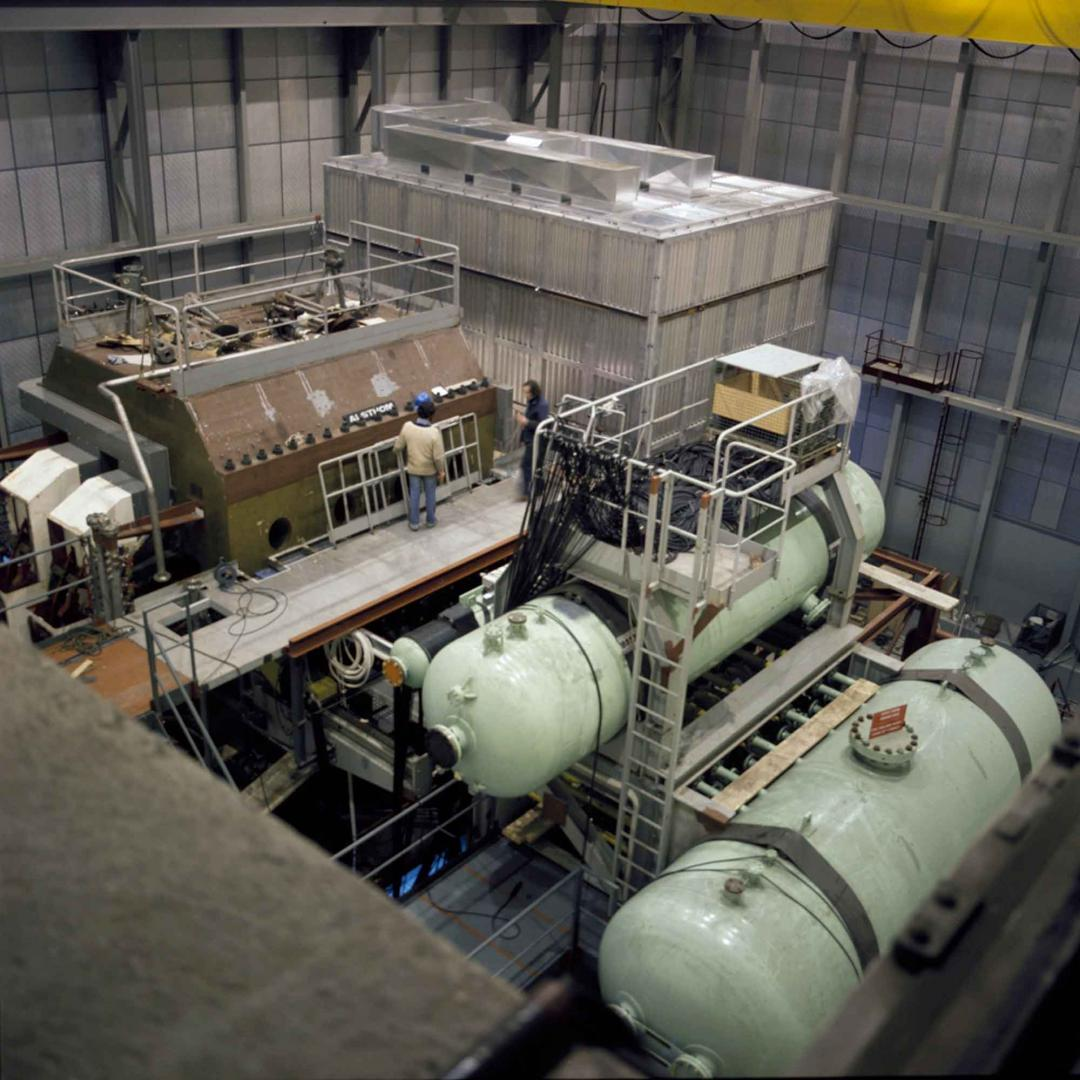
\includegraphics[width=\marginparwidth]{SM/gargamelle.jpg}
	\captionof{figure}{Gargamelle.}
	\label{GARGAMELLE}
}
\marginpar
{
	\centering
	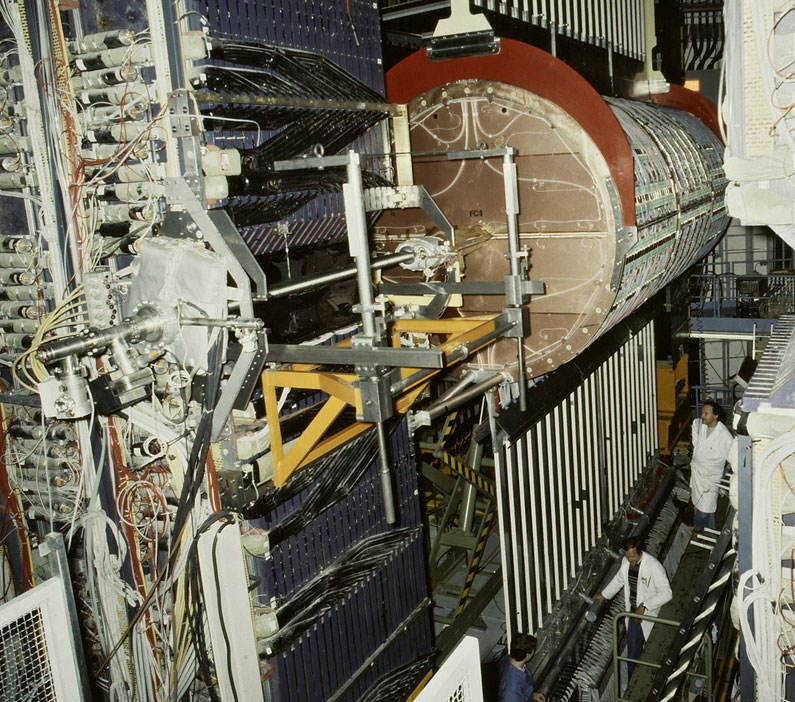
\includegraphics[width=\marginparwidth]{SM/ua1.jpg}
	\captionof{figure}{UA1.}
	\label{UA1}
}
\marginpar
{
	\centering
	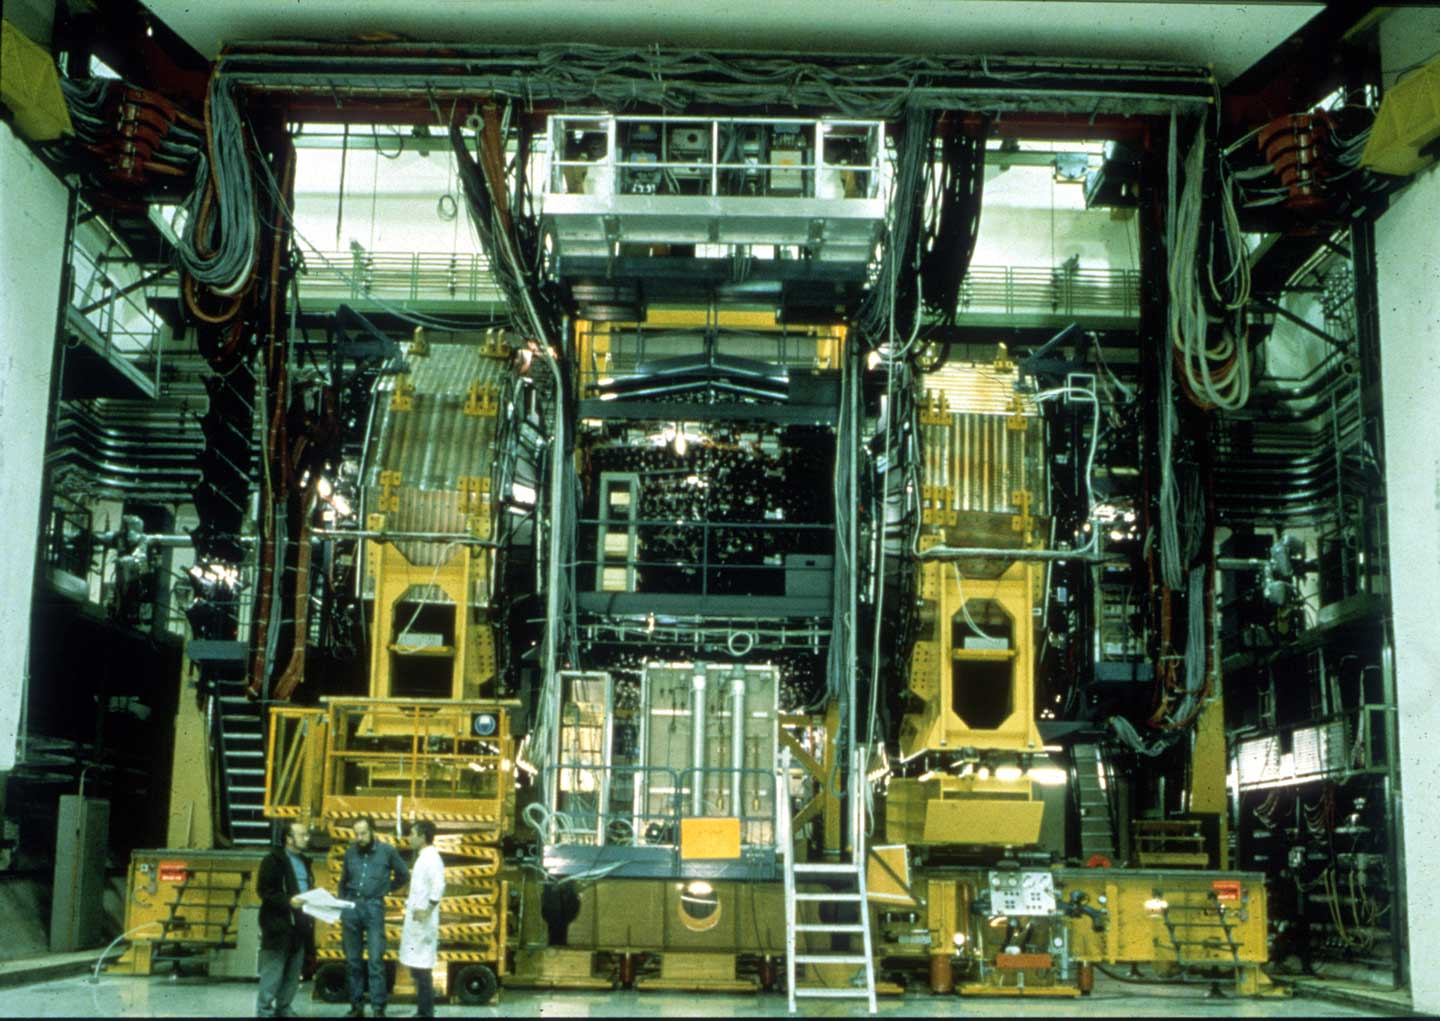
\includegraphics[width=\marginparwidth]{SM/ua2.jpg}
	\captionof{figure}{UA2.}
	\label{UA2}
}
\marginpar
{
	\centering
	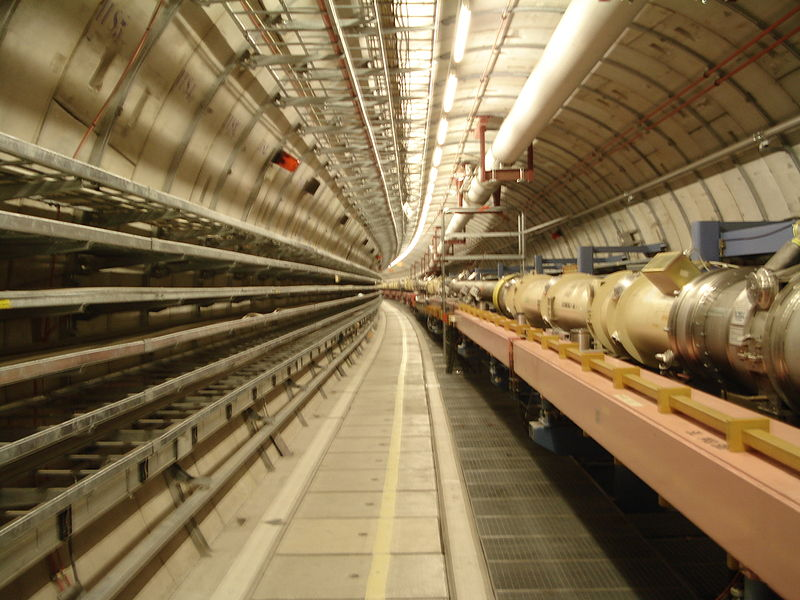
\includegraphics[width=\marginparwidth]{SM/HERA.jpg}
	\captionof{figure}{tunnel du collisionneur HERA.}
	\label{HERA}
}
\marginpar
{
	\centering
	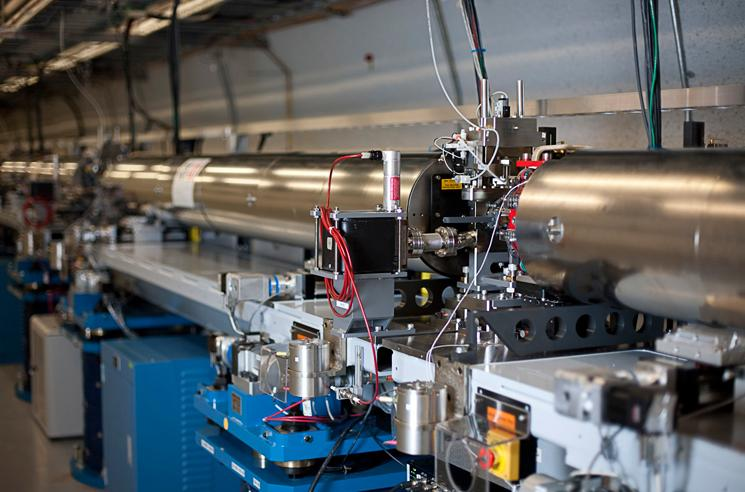
\includegraphics[width=\marginparwidth]{SM/slac.jpg}
	\captionof{figure}{Beam line du SLAC.}
	\label{SLAC}
}

De plus l'ensemble des mesures effectuées jusqu'à présent sont compatibles avec le Modèle Standard: La figure (fig.\ref{mesures}) montre la mesure de certains paramètres ainsi que leur "pull" défini par :
\begin{equation}
\frac{O^{mesure}-O^{fit}}{\sigma^{mesure}}
\end{equation}
c'est à dire la déviation entre les mesures expérimentales et les prédictions théoriques en unités de l'incertitude expérimentale. Tous les pulls sont inférieur à $3\sigma$. L'expérience et la théorie sont donc en très bon accord.

\begin{figure}[h!]
\centering
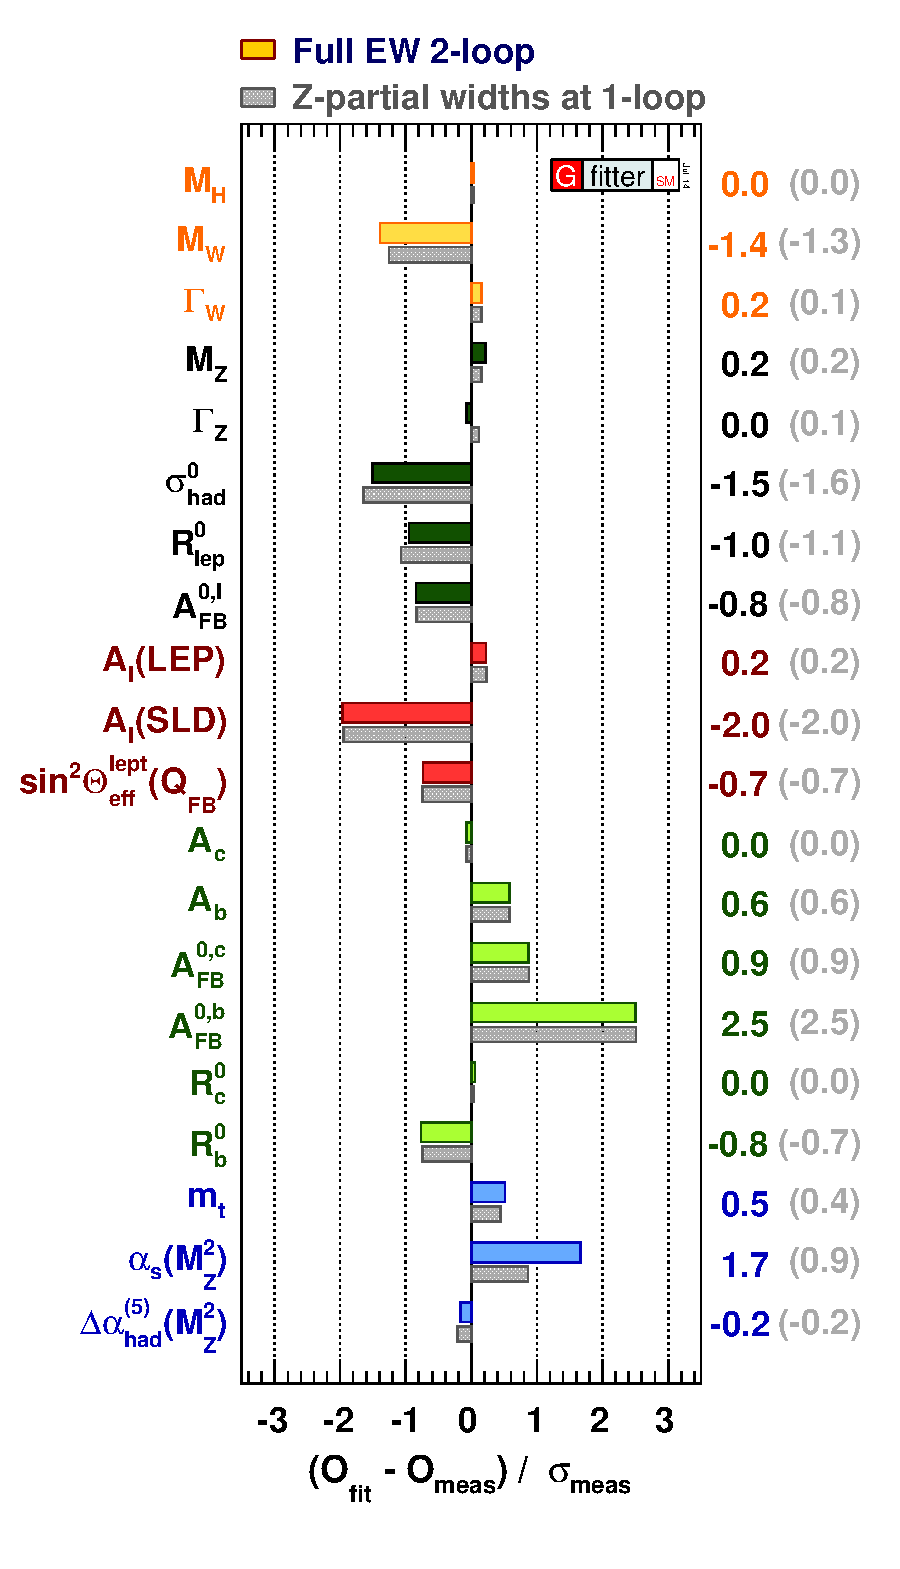
\includegraphics[width=0.50\textwidth]{SM/mesure.eps}
\captionof{figure}{Comparaison des résultats d'ajustement avec les mesures directes de certains paramètres du Modèle Standard.}
\label{mesures}
\end{figure}

\section{Les faiblesses du Modèle Standard}
Le modèle Standard est en accord remarquable avec l'expérience. Cependant, plusieurs problèmes et questions non résolubles amène à considérer le Modèle Standard comme une théorie effective, valable jusqu'à l'échelle du TeV. Une nouvelle physique qui engloberait le Modèle Standard devrait apparaitre à cette échelle d'énergie.

Parmis les principaux problèmes ou faits inexpliqués par le Modèle Standard, on peut citer :
\begin{itemize}[label=$\bullet$]
\item \textbf{Les neutrinos massifs :}
\marginpar
{
\centering
\includegraphics[width=\marginparwidth]{SM/kamiokande.jpg}
\captionof{figure}{Intérieur du détecteur Super-Kamiokande.}
\label{kamiokande}
}
\marginpar
{
\centering
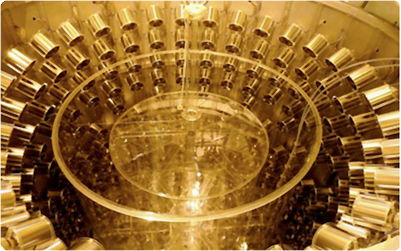
\includegraphics[width=\marginparwidth]{SM/chooz.jpg}
\captionof{figure}{Coeur du détecteur Double Chooz.}
\label{chooz}
} 
Les expérience Super-Kamiokande\ref{kamiokande} et GALLEX portant sur l'observation du flux de neutrinos provenant du Soleil et les expériences Double Chooz\ref{chooz} et K2K pour les flux de neutrinos de sources artificielles terrestres ont mis en évidence l'oscillation des neutrinos entre les saveurs leptoniques. Ces oscillations ne peuvent s'expliquer que si les neutrinos sont massifs et s'il existe des neutrinos droits. Bien que le Modèle Standard considére les neutrinos comme des particules de masse nulle et que de parité gauche, il est facile d'y ajouter un neutrino droit dans chaque famille et les couplages au doublet Higgs correspondant afin de rendre compte de ces faits expérimentaux\footnote{C'est d'ailleurs cette extension du Modèle Standard qui est présenté dans ce chapitre.}. Cependant cela aggrave le problème de la hiérarchie des masses car les masses des particules élémentaires s'étalent sur 10 ordres de grandeur !

\item \textbf{Le nombre de paramètres libres :} Le modèle standard contient 18 paramètres libres : les 3 constantes de couplages, les deux paramètres $\lambda$ et $\mu^2$ du potentiel de Higgs, 9 couplages de Yukawa et les trois angles et une phase pour les quarks dans la matrice CKM ainsi que l'angle associé auwx. Et d'autres encore en ajoutant le fait que les neutrinos soit massif.

\item \textbf{Le nombre de familles :} Le nombre de famille a été expérimentalement obtenu en comparant la section efficace hadronique en fonction de l'énergie du centre de masse expérimentale au prédiction théorique différents nombres de familles de neutrinos de masse négligeable. Actuellement on considère que trois familles\ref{neutrinos}. Cependant le fait que les neutrinos soient massif permet l'existance de plus de trois familles si les neutrinos on une masse supérieur à $m_{Z^{0}}/2$.
\begin{figure}[h!]
\centering
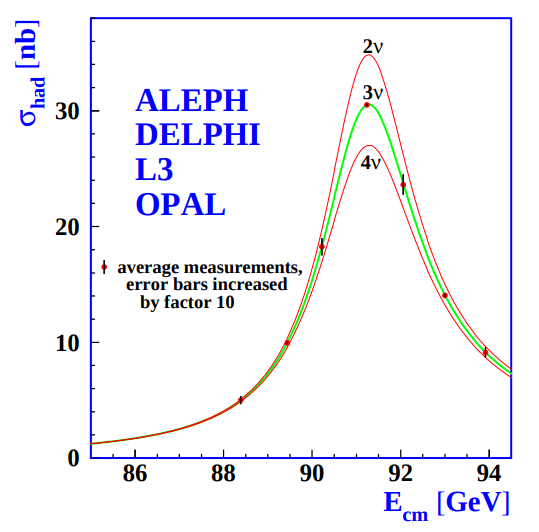
\includegraphics[width=0.48\textwidth]{SM/neutrinos.png}
\captionof{figure}{Mesures de la section efficace de production hadronique près de la résonance en Z. Les courbes indiquent les sections efficaces prédites pour deux,trois et quatres espéces de neutrinos avec les couplages du Modèle Standard et de masses négligeables.}
\label{neutrinos}
\end{figure}

\item \textbf{La baryogénèse :} Le Modèle Standard est incapable d'expliquer l'asymétrie entre la quantité de baryons (matière) et d'anti-baryons (anti-matière) observés dans l'Univers.

\item La gravitation : Le Modèle Standard ne comporte pas l'interaction gravitationnelle. Aucune formulation quantique de la gravitation n'a encore été trouvé. La meilleur théorie gravitationnelle, la relativité générale et malheureusement incompatible avec le Modèle Standard.

\item \textbf{Le problème de naturalité :} En effet, il paraît naturel de considérer une échelle d'énergie ou le Modèle Standard cesse d'être valide. Or, les ordres supérieur de la théorie perturbative ajoutent des corrections radiatives aux masses des différentes particules. En imposant une échelle d'énergie à la validité du Modèle Standard $\Lambda$, un "cut-off", les corrections vont en dépendre. Pour le boson de Higgs et en considérant les diagramme de la figure fig.\cref{corrections} on peut écrire :
\begin{equation}
m_{h}^{2}=m_{0}^{2}-\delta m_{h}^{2}
\end{equation}
avec $m_{0}^{2}$ la masse "nue" du boson, $m_{h}^{2}$ la masse effective et $\delta m_{h}^{2}$ les corrections radiative.
\begin{figure}[h!]
\centering
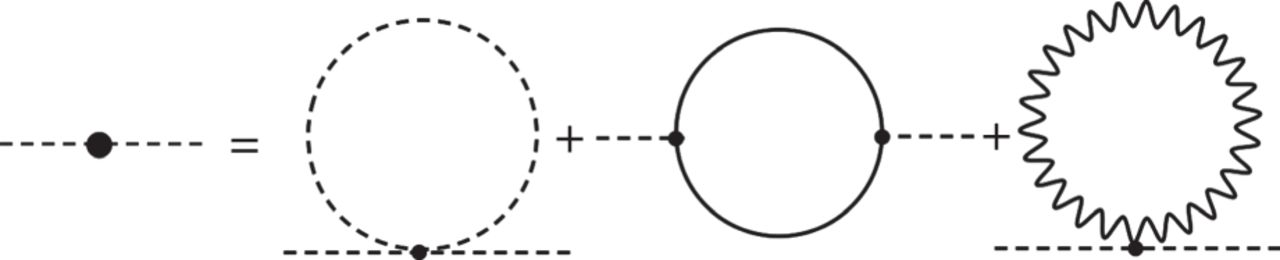
\includegraphics[width=0.40\textwidth]{SM/corrections.jpg}
\captionof{figure}{Correction radiative du premier ordre pour le boson de Higgs.}
\label{corrections}
\end{figure}
La contribution fermionique est de la forme :
\begin{equation}
\label{eq1}
\delta m_{h}^{2}=-\frac{y_{f}^{2}}{16\pi^{2}}\left(2\Lambda^{2}+6m_{f}\log\left(\frac{\Lambda}{m_{f}}\right)\cdots\right)
\end{equation}
En considérant un cut-off de l'ordre de $\Lambda \sim 10^{16}$GeV il faut donc un accord à $10^{-30}$ entre $m_{0}^{2}$ et $\delta m_{h}^{2}$. Ce problème de hiérarchie, et de réglage fin des paramètres ne semble pas naturel.

\item \textbf{La Matière Noire et l'Énergie Noire} : Des observations cosmologiques ont mis en évidence la présence de matière dite noire car elle n'émet pas et n'interagît pas avec les radiations électromagnétiques. Bien que n'ayant jamais été directement observé, son existence et certaines de ses propriétés peuvent être étudiés par leur effets gravitationnelles sur le mouvement de la matière visible, elle serait  également à l'origine de la formation des galaxies et des amas de galaxies, et de leurs répartition de façon non uniforme dans l'Univers. D'après les observations du satellite Plank\ref{Plank},
la matière que nous connaissons ne compose que 4.9\% du totale mass-énergie de l'Univers. La matière noire quant à elle ne compte que pour 26.8\%. Les 68.3\% restant sont composés d'énergie noire. Cette énergie serait responsable de l'accélération de  l'expansion de l'Univers qui à été mis en évidence en 1998 par les projets Supernova Cosmology Project et High-Z supernovae search team. Ni la matière noire ni l'énergie noire ne sont décrites par le Modèle Standard.
\marginpar
{
\centering
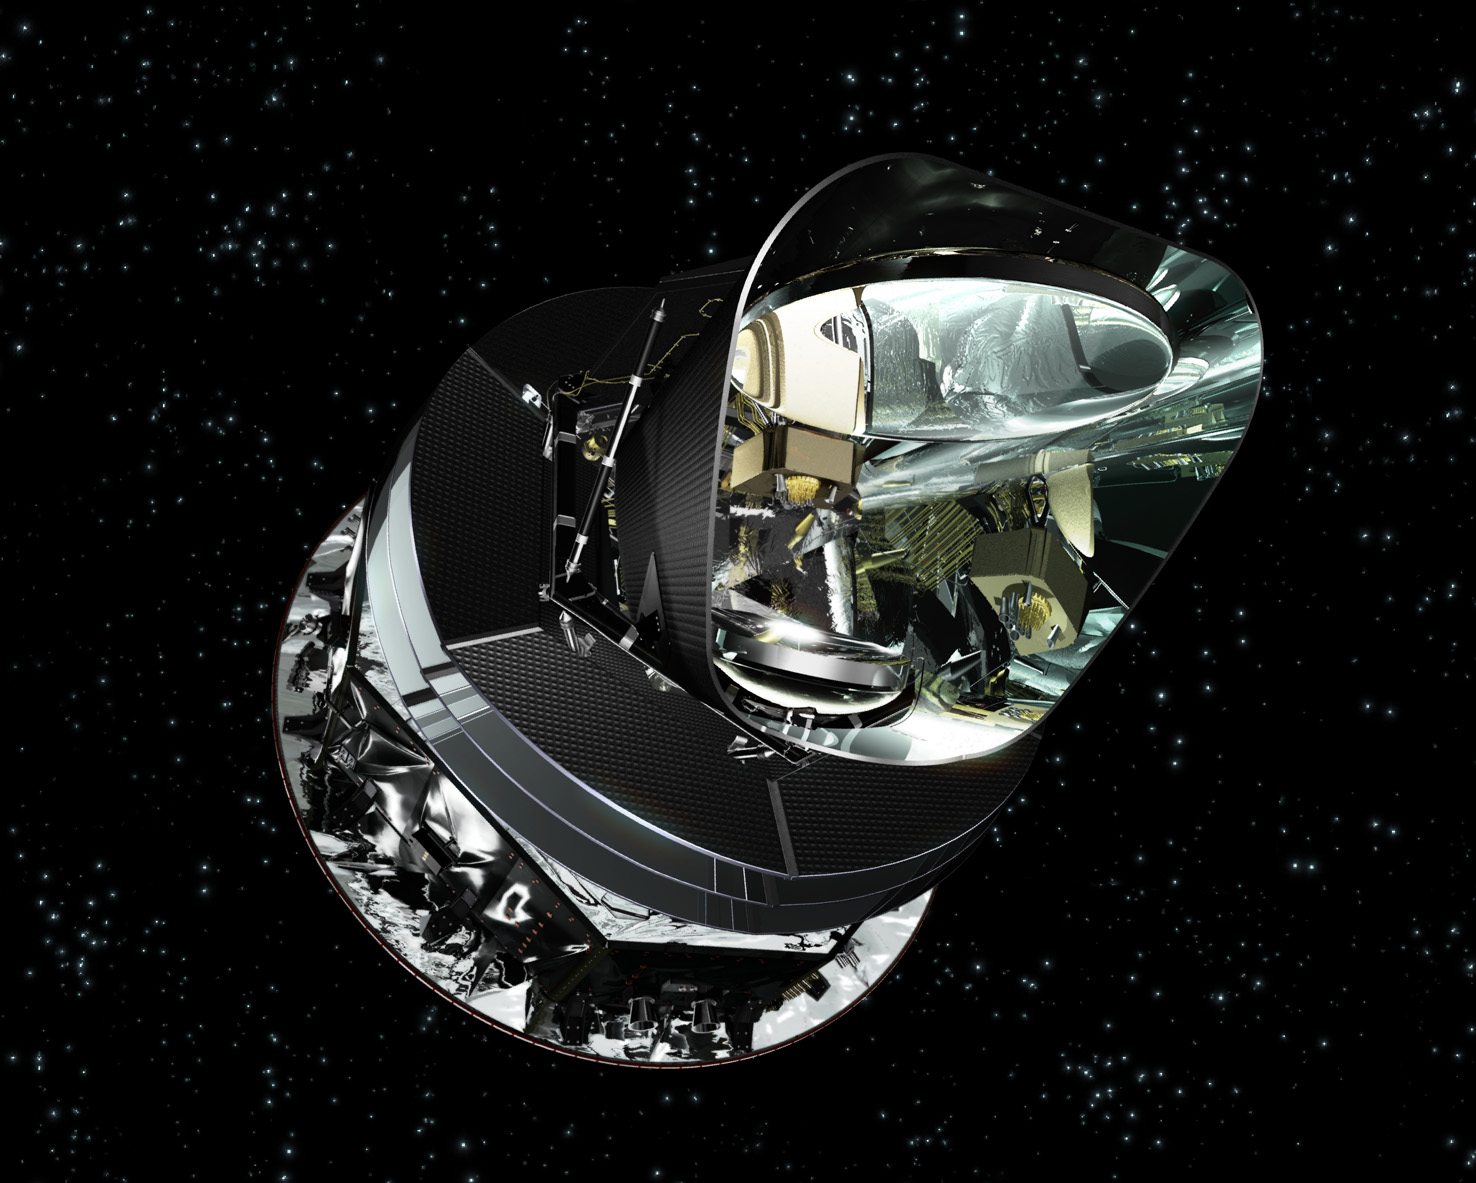
\includegraphics[width=\marginparwidth]{SM/plank.jpg}
\captionof{figure}{Le satellite Plank.}
\label{Plank}
} 

\item \textbf{La non unification des couplages : }Les constantes de couplages $\alpha_{1}$,$\alpha_{1}$ et $\alpha_{3}$ respectivement de l'interaction electromagnétique, faible et forte dépendent de l'échelle d'énergie. Il s'avére que ces trois constantes se rapprochent l'une de l'autre à haute énergie mais ne concourent pas en un seul point (cf.fig\ref{constantes}). Bien que n'étant pas en soit un problème, la convergence vers une valeur unique à haute énergie et nécessaire à une théorie "du tout" qui unifierait ces trois interactions. Le calcul de l'évolution de ces constantes par la méthode de renormalisation n'aboutissant pas à la convergence de ces trois constantes tend à prouver une lacune du Modèle Standard et son caractère effectif.
\begin{figure}[h!]
\centering
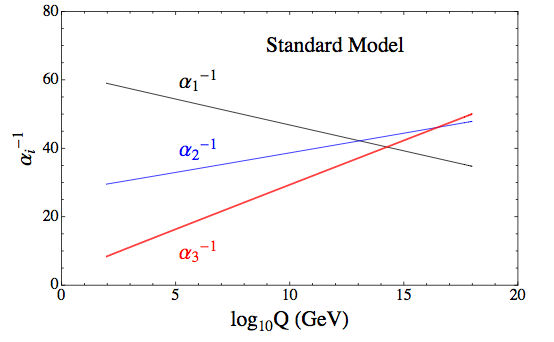
\includegraphics[width=0.50\textwidth]{SM/couplageSM.jpg}
\captionof{figure}{Évolution des constantes de couplage en fonction de l'échelle d'énergie dans le cas du Modèle Standard.}
\label{constantes}
\end{figure}
\end{itemize}

\section{Au delà du Modèle Standard}
Afin de résoudre certains de ces problèmes, de nombreux modèles théorique ont été développé, cependant aucun d'entre eux n'est capables de répondre à toutes les questions et combler les lacunes du Modèle Standard. Certaines de ces théorie sont des extensions du à ce modèle, d'autre propose des modèles complètement différents.

La majorité des modèles repose sur les symétries du Modèle Standard et cherche à les étendre : Soit en trouvant d'autres symétries internes (Grand Unified Theorries (GUT)), soit en liant les symétries internes et externes ( supersymétrie (SUSY)) voir même modifier la nature même de l'espace temps en ajoutant des dimensions supplémentaires par exemple.

\subsubsection{Les modèles de grande unification}
Ces modèles s'appuient sur le fait qu'il ait été possible de réunir dans le Modèle Standard trois des quatre interactions que nous connaissons et que leur constantes de couplage se rapprochent l'une de l'autre à haute énergie. Il semble donc logique de vouloir unir ces trois interactions sous une même symétrie. Il n'existerait alors plus qu'un groupe G et qu'une seule constante de couplage. Ces théories doivent bien sûr être renormalisables et leur groupe doit avoir comme sous groupe celui du Modèle Standard $SU(3)\otimes SU(2) \otimes U(1)$. Les groupes $SU(5)$ et $SO(10)$ ont notamment été étudié.

\subsubsection{Modèles à dimensions supplémentaires}
Ces modèles tentent de supprimer la naturalité et la hiérarchie des échelles d'énergies en faisant tendre l'échelle de Planck vers celle de l'interaction faible. Pour cela ils prennent comme hypothèse que l'espace temps contient des dimensions supplémentaires enroulées compacts. L'interaction gravitationnelle évolue donc dans ces dimension supplémentaires.

\subsubsection{La supersymètrie}
La supersymètrie a été introduite par Weiss et Zumino en 1974. Elle consiste à supprimer les divergences quadratiques  en les annulant grâce à l'ajout de termes supplémentaires. Pour cela on associe à chacun des fermions $f_{L}$ et $f_{R}$ un partenaire scalaire $\tilde{f}_{L}$ et $\tilde{f}_{R}$ possédant les mêmes nombres leptoniques et baryoniques. Ces partenaires contribuent donc aux diagramme de correction radiative de la masse du Higgs (cf.fig\ref{corrections}). Les boucles scalaires ont une contribution positive contrairement aux boucles fermioniques, il est ainsi possible de supprimer le terme en $\Lambda^2$ de la formule (\ref{eq1}). La masse du Higgs est varie alors comme le logarithme de l'énergie $\Lambda$. On supprime ainsi le problème du fine-tuning et de la naturalité. Les équations de renormalisation sont également modifiées et il est possible de faire concourir les constantes de couplages en un point. La supersymètrie est donc également un candidat à une théori du "tout". La supersymètrie souffre cependant de certains problèmes, en effet, les particules superpartenaires sont censé être de même masse que les particules élémentaires. Or aucune superparticule n'a encore été detécté expérimentalement. Il faut donc introduire un mécanisme de brisure de la supersymètrie.

Nombres de ces théories postulent l'existence de nouvelles particules ou d'effets qui peuvent être vérifier expérimentalement. Pour pouvoir savoir laquelle de ces théories décrit au mieux la la nature ou contraindre ces modèles, il est nécessaire de construire de nouveaux accélérateurs toujours plus puissant et des détecteurs de plus en plus perfectionnés. 

\chapter{Le Grand collisionneur de hadrons (LHC)}
\renewcommand\chapterillustration{LHC/lhc}
\ThisULCornerWallPaper{1}{\chapterillustration}
\minitoc
\lettrine[lines=4, slope=-0.5em]{C}{e} chapitre décrit le complexe des accélérateurs du CERN\footnote{Organisation Européenne pour le Recherche Nucléaire (Laboratoire européen de physique des particules)} qui permet d'accélérer les particules, afin d'avoir un faisceau de particules avec une énergie suffisante pour être injecté dans le Grand Collisionneur de Hadrons (LHC\footnote{Large Hadron Collider}) et atteindre une énergie finale de $7$ TeV. Cette description bien que succincte est nécessaire car de nombreux résultats obtenus durant cette thèse ont nécessité l'utilisation d'accélérateurs de ce complexe. Une description du LHC est également donnée, car ses performances présentes et futures déterminent les choix technologiques des détecteurs utilisant son faisceau.

\section{Le complexe d'accélérateurs du CERN}

Le complexe d'accélération (\ref{complexe}) du CERN est une série de machines qui délivrent des faisceaux de particules d'énergies de plus en plus élevées. Chaque machine accélère les faisceaux et les injecte dans la machine suivante. Le dernier accélérateur du complexe est le LHC.

Le programme de ce dernier est surtout basé sur des collisions protons-protons. Cependant chaque année, environ un mois est consacré aux collisions d'ions lourds (plomb-plomb) ou (proton-plomb) afin d'étudier notamment le plasma de quarks et gluons, l'une des phases de l'Univers peu après le Big Bang. 

Dans le cas de ces collisions, la chaine d'accélération est constituée du Linear Accelerator 3 (LINAC 3), du Low Energy Ion Ring (LEIR) utilisé pour le stockage des ions et leur refroidissement. La chaine d'accélération est ensuite identique à celle pour les collisions proton-proton.

\begin{minipagewithmarginpars}[h]{\textwidth}
  	\centering
	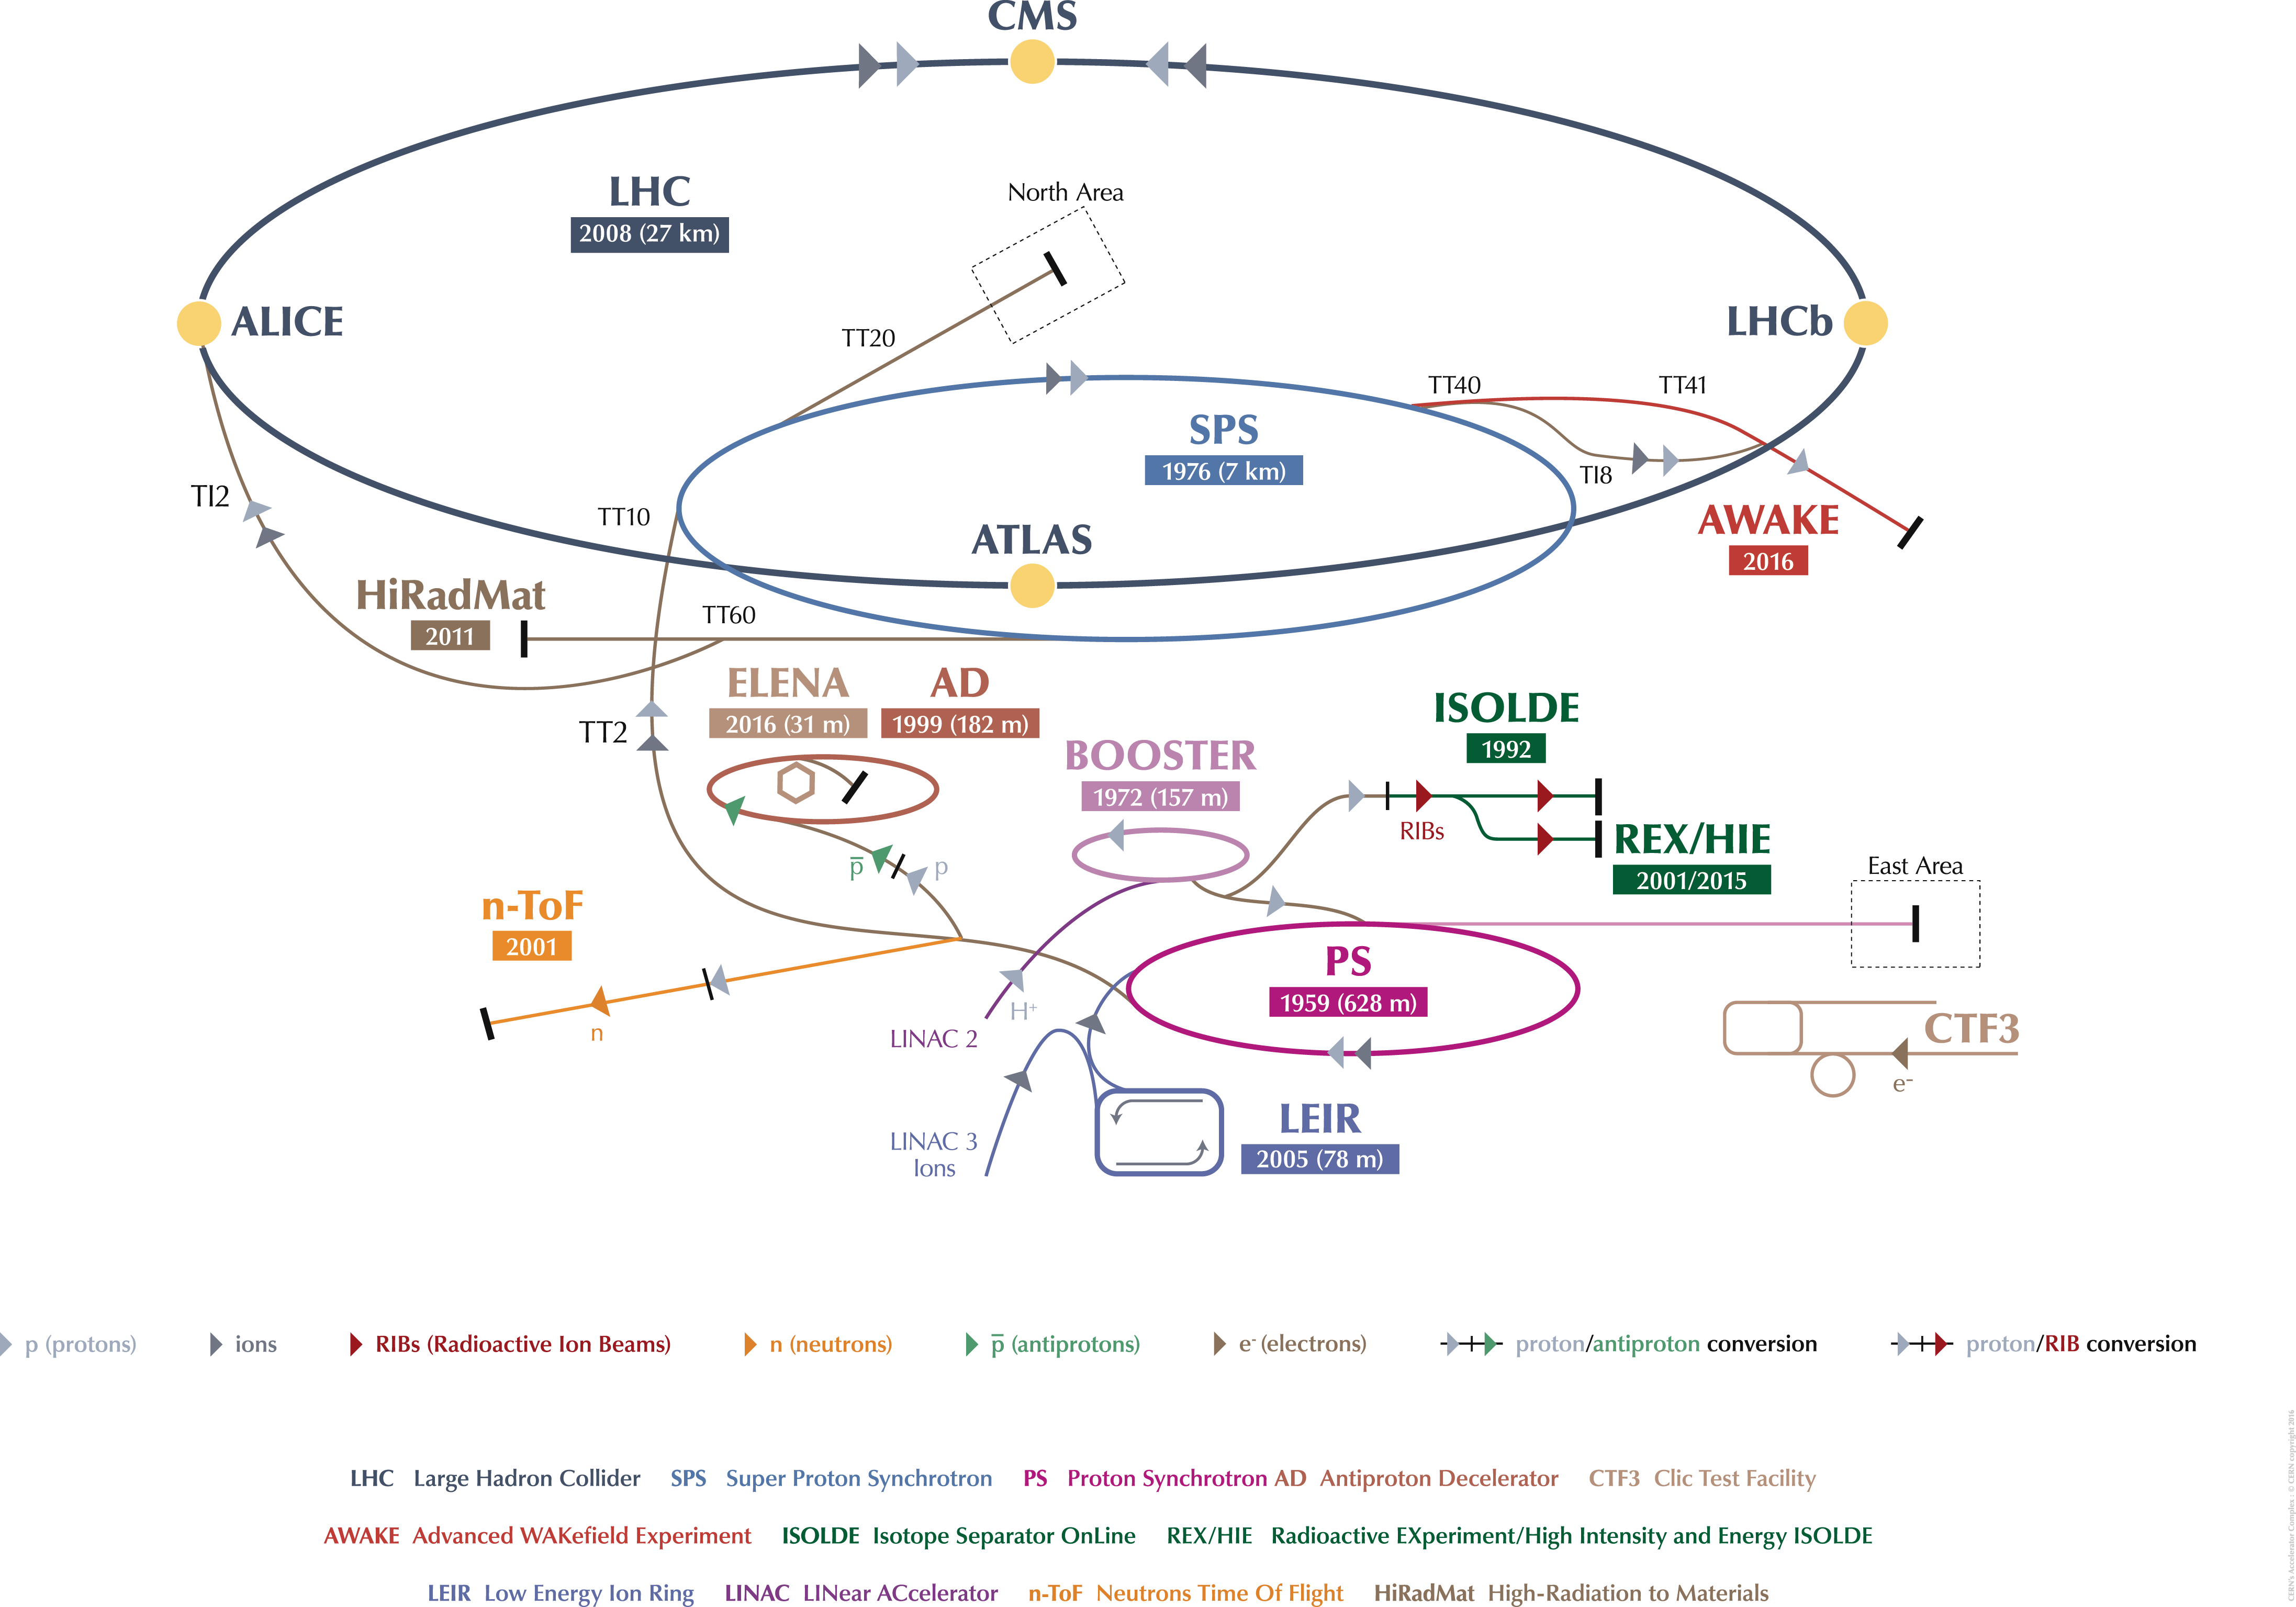
\includegraphics[scale=0.25]{LHC/complexe.png}
  	\captionof{figure}{Schéma du complexe d'accélération du CERN. La chaine d'injection du LHC est constituée du Linac 2, du Booster, du PS et du SPS}
  	\label{complexe}
  	\par 	
\marginpar
{
	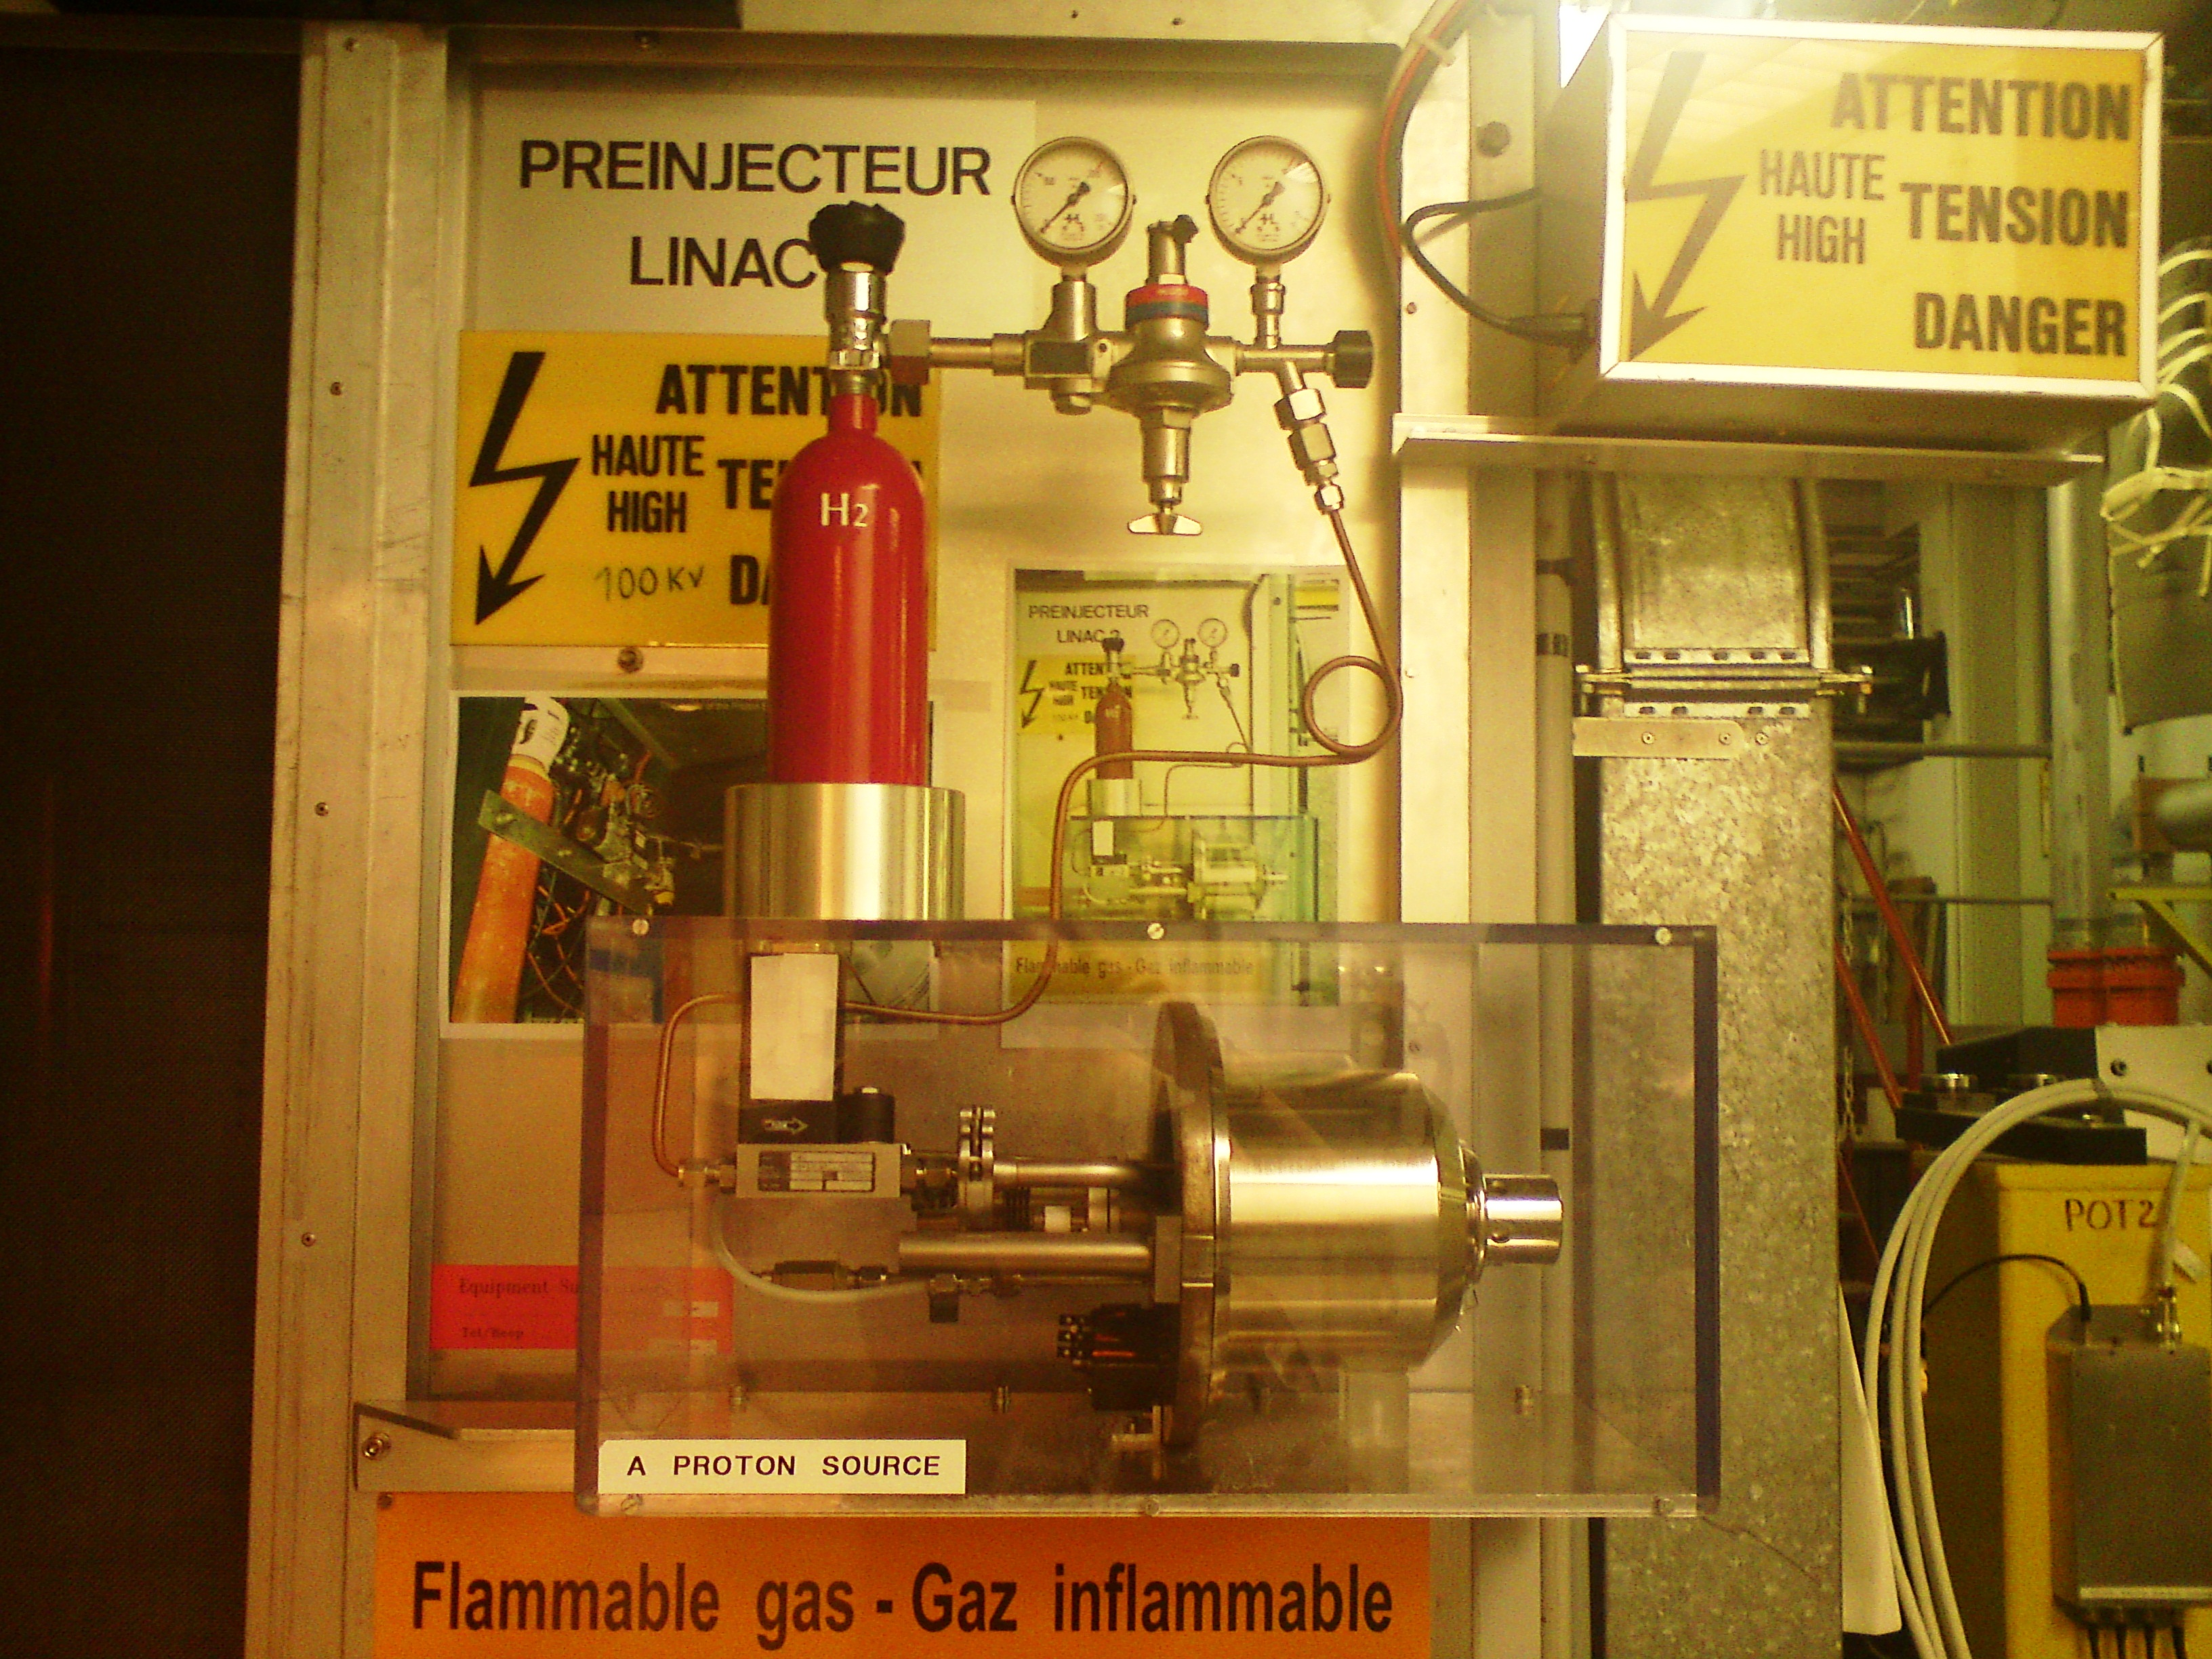
\includegraphics[width=\marginparwidth]{LHC/Bouteille.jpg}
	\label{bouteille}
    	\captionof{figure}{Source des protons du LHC.}
}	
\end{minipagewithmarginpars}

\marginpar
{
	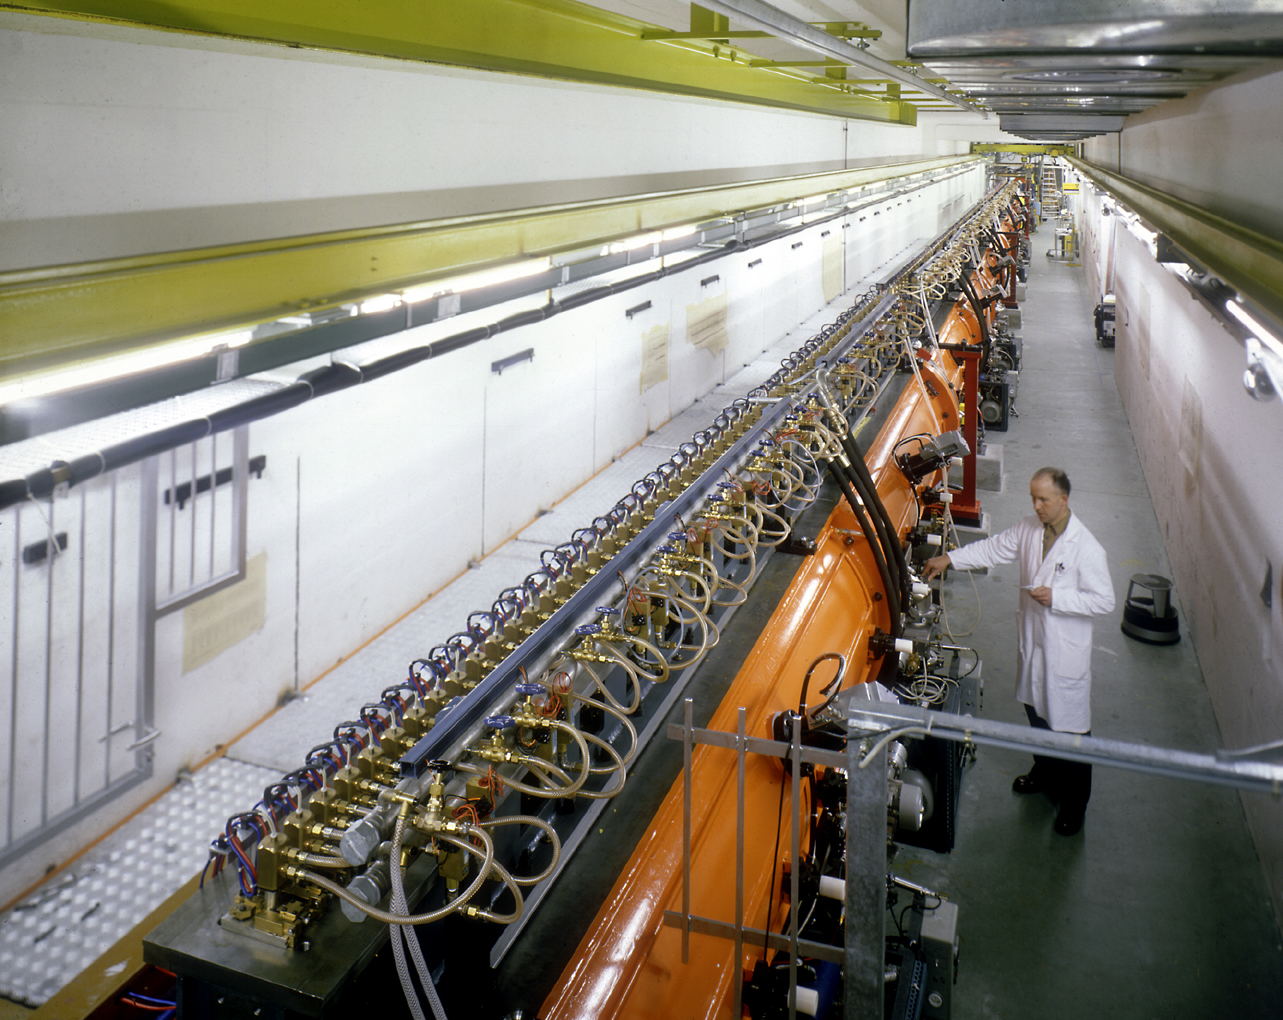
\includegraphics[width=\marginparwidth]{LHC/linac2.jpg}
    \captionof{figure}{Photo du LINAC 2.}
    	\label{linac2}
}

\marginpar
{
	
	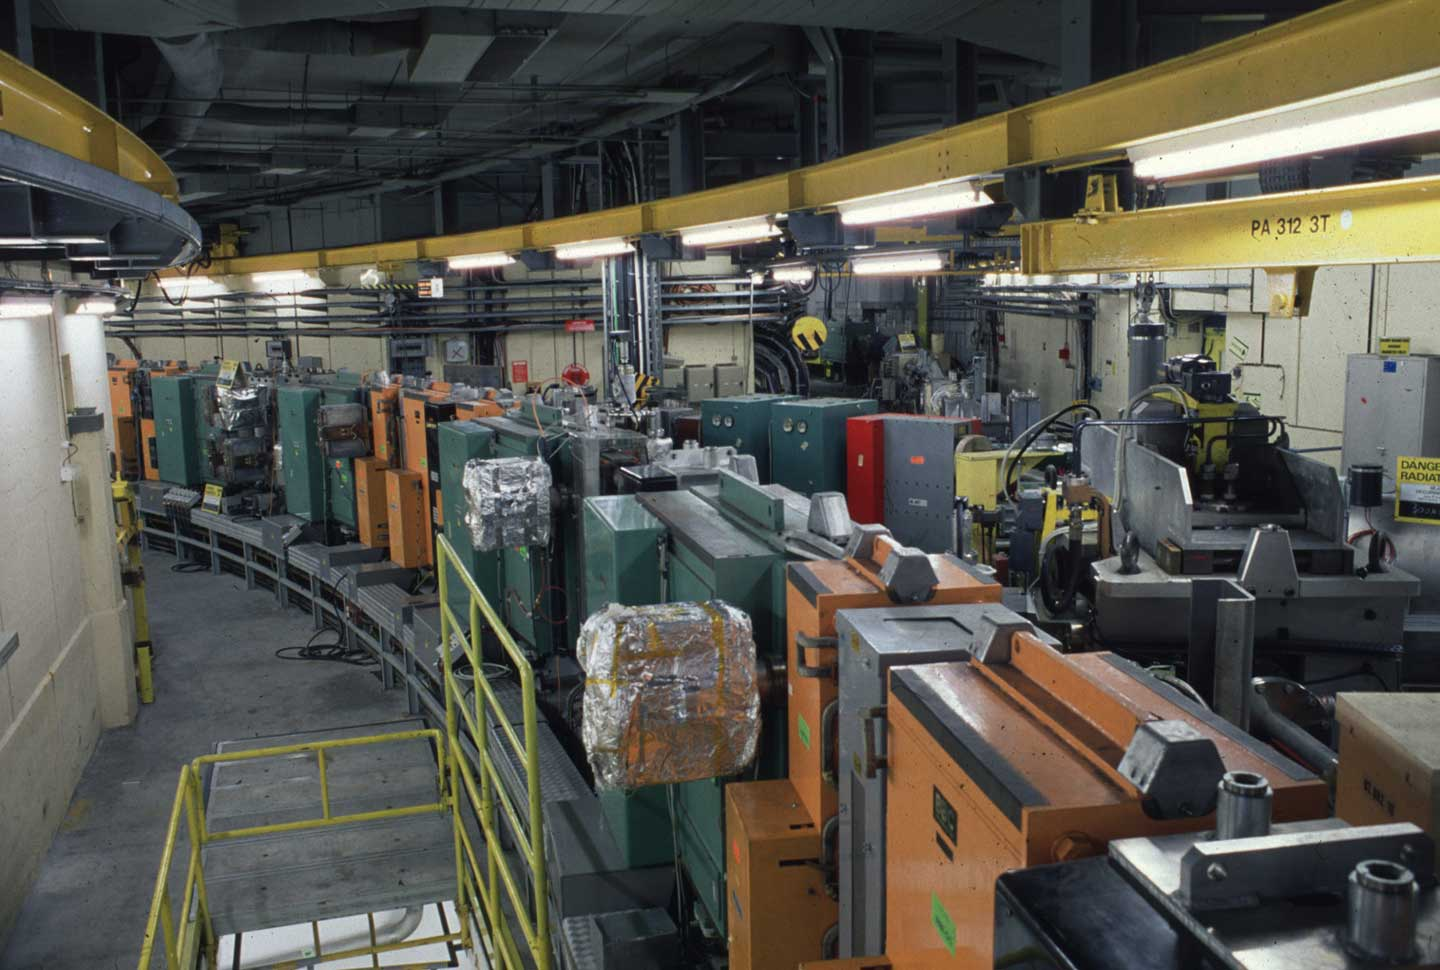
\includegraphics[width=\marginparwidth]{LHC/booster.jpg}
    \captionof{figure}{Photo du Booster du Synchrotron à protons.}
    	\label{booster}
}

\marginpar
{
	
	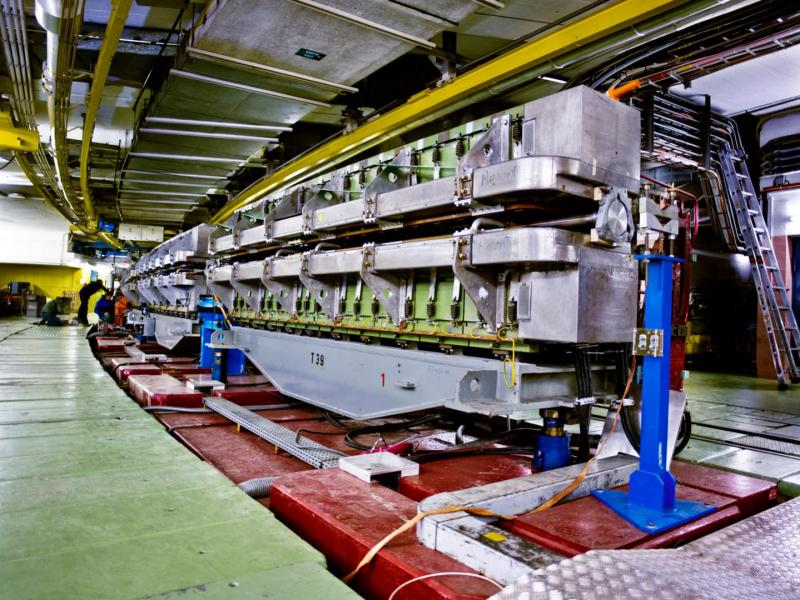
\includegraphics[width=\marginparwidth]{LHC/ps.jpg}
    \captionof{figure}{Photo du PS.}
    	\label{ps}
}

\marginpar
{
	
	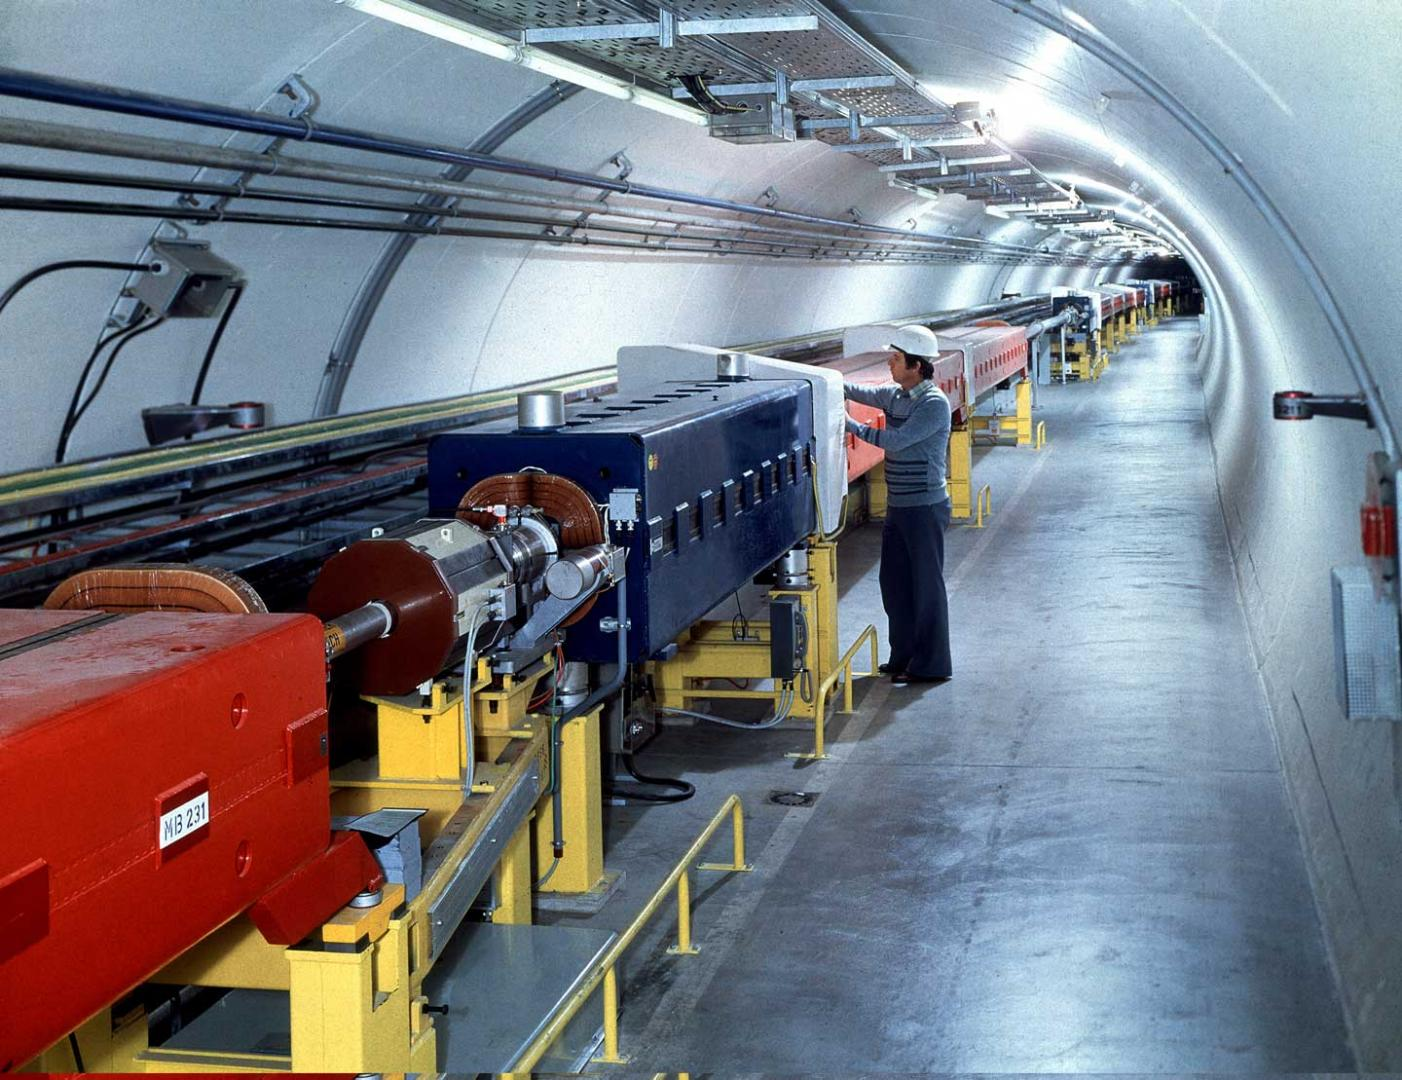
\includegraphics[width=\marginparwidth]{LHC/sps.jpg}
    \captionof{figure}{Photo du SPS.}
    	\label{sps}
}
Pour les collisions proton-proton, la source de protons est une bouteille de dihydrogène gazeux (fig. \ref{bouteille}). Les atomes d’hydrogène sont soumis à un champ électrique, qui arrache leurs électrons et les ionise en $H^{+}$ (proton). Les protons extraits sont ensuite envoyés dans l'accélérateur linaire (LINAC 2 (fig. \ref{linac2})) où ils atteignent l'énergie de 50 MeV et sont $5\%$ plus massifs. Ils passent ensuite dans les 4 anneaux de 157m de circonférence du Booster du Synchrotron à protons (BOOSTER (fig. \ref{booster})) qui les amènent à une énergie de 1.4 GeV avant de les injecter dans l'accélérateur suivant, le Synchrotron à protons (PS (fig. \ref{ps})). Cet accélérateur circulaire de 628 mètres de circonférence, permet aux faisceaux d'atteindre une énergie de 25 GeV. Il sert aussi à préparer le faisceau en le découpant en série de paquets (bunchs) de particules nécessaires au LHC. Ces bunchs sont ensuite envoyés dans le supersynchrotron à protons (SPS (fig. \ref{sps})) d'une circonférence de 7 km, où l'énergie du faisceau atteint 450 GeV. Les paquets sont regroupés pour former des trains de paquets avant d'être enfin envoyés dans le Grand Collisionneur de Protons (LHC). L'injection et le guidage de faisceaux d'une telle énergie par des aimants supraconducteurs rapides est une tâche délicate et pourrait détériorer l'accélérateur. Un faisceau de test de faible intensité "pilot beam" est donc injecté afin de mesurer et vérifier les paramètres. Le faisceau de haute énergie est ensuite séparé en deux et injecté dans deux conduits différents, l'un circulant dans un sens et l'autre dans le sens contraire. Ces faisceaux sont ensuite accélérés jusqu'à une énergie de 7 TeV et ne se croisent qu'aux points d'intéractions.

\section{Le Large Hadron Collider}
Le LHC est le dernier accélérateur circulaire du complexe d'accélération. Il utilise le tunnel de 27 km de circonférence situé à une centaine de mètres sous terre. Il fût construit pour acceuillir le Grand collisionneur électron-positron (LEP\footnote{Large Electron Positron collider.}), qui fût en service de 1989 à 2000. Le LHC à été mis en service en 2008 et a été construit afin de produire de l'ordre de 600 millions de collisions proton-proton par seconde à une énergie au centre de masse de $\sqrt{s}=14$ TeV. Il est actuellement l'accélérateur de proton-proton le plus puissant du monde, et a permis de mettre en évidence l'existence du boson de Higgs, dernière pièce manquante du Modèle Standard.

Le LHC est un collissioneur de particules non fondamentales (hadrons) à l'inverse de son prédécesseur, le LEP qui utilisé des électrons et des positrons. Lors d'une collission entre hadrons, ceux sont ses constituant élementaires, les quarks et les gluons qui collissionnent entre eux. Ceux-ci possèdent seulement une portion de l'énergie du hadrons qui les contient. L'énergie du centre de masse de cette collision n'est donc pas connue avec précision. Le LHC est donc une machine de découverte de particules plutôt qu'une machine de mesures de précisions comme l'était le LEP, car il permet d'acceder à un large spectre en énergie. Généralement, les mesures de précision sont effectué grâce à des collisionneur utilisant des particules élémentaires ($e^{-}$,$e^{+}$); ils sont dans ce cas souvent linéaire afin d'éviter la perte d'énergie par rayonnement synchroton.

La figure \ref{lhcschema} est une vue schématique du LHC. En vérité le LHC n'est pas parfaitement circulaire, mais est composé de $8$ octants composés d'une section droite de longueur $~5$ km et d'un secteur courbe d'une longueur de $~3$ km (fig. \ref{octants}). Les sections droites sont utilisées afin de faire collisionner les deux faisceaux de protons venant en sens inverse l'un de l'autre. Il existe $8$ points potentiels d'interactions (P), mais seulement $4$ sont le siège de collisions et possèdent des détecteurs qui analysent les données issues de ces collisions : le point P1 pour ATLAS\footnote{A Toroidal LHC ApparatuS, détecteur généraliste.}, le point P2 pour ALICE\footnote{A Large Ion Collider Experiment, dédié à l'étude du plasma de quarks et gluons.}, le point P5 pour CMS\footnote{Compact Muon Solenoid, détecteur généraliste.} et le point P8 pour LHCb\footnote{Large Hadron Collider beauty experiment, dédié au quark b.}.

\begin{minipagewithmarginpars}[h]{\textwidth}
  	\centering
	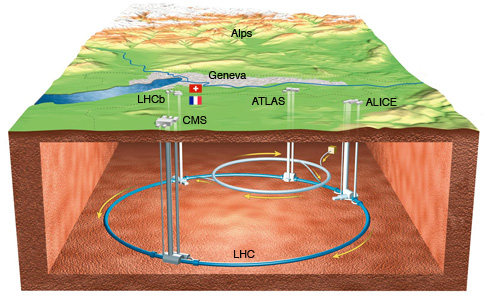
\includegraphics[scale=0.6]{LHC/CERNMap.jpg}
  	\captionof{figure}{Vue schématique du LHC.}
  	\label{lhcschema}
  	\par 	
\marginpar
{
	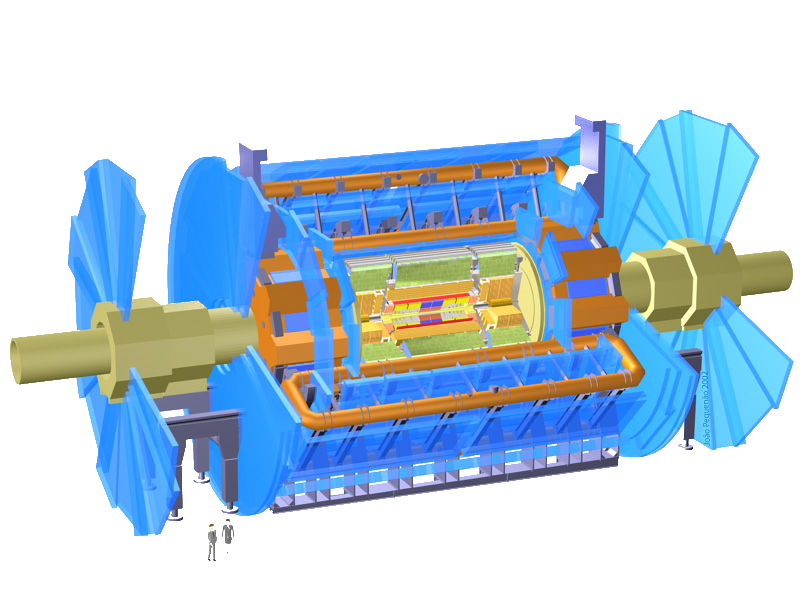
\includegraphics[width=\marginparwidth]{LHC/atlas.png}
    \captionof{figure}{ATLAS.}
    	\label{atlas}
}
\end{minipagewithmarginpars}

\begin{minipagewithmarginpars}[h]{0.95\textwidth}
  	\centering
	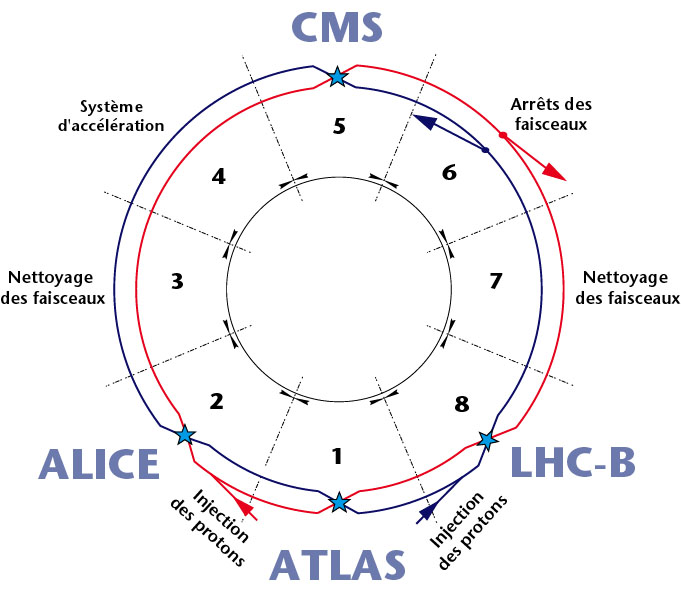
\includegraphics[width=0.55\textwidth]{LHC/lhc-schematic.jpg}
  	\captionof{figure}{Vue schématique des octants du LHC ainsi que des positions des principaux détecteurs le long du LHC. Les faisceaux (en bleu et rouge) circulent en sens inverse l'un de l'autre.}
  	\label{octants}	
  	\par 	
\marginpar
{
    \vspace*{-7.5cm}
	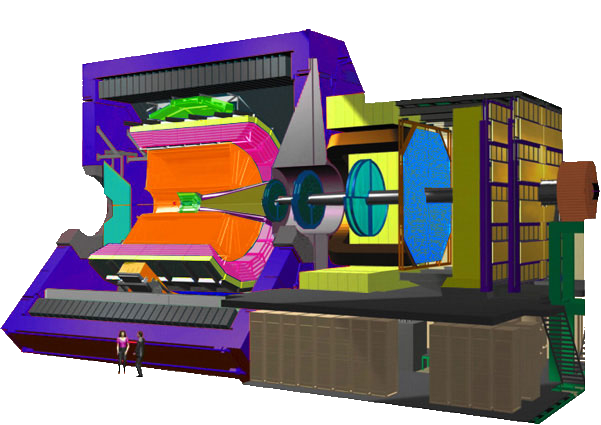
\includegraphics[width=\marginparwidth]{LHC/alice.png}
    \captionof{figure}{ALICE.}
    	\label{alice}
}
\end{minipagewithmarginpars}
\marginpar
{
	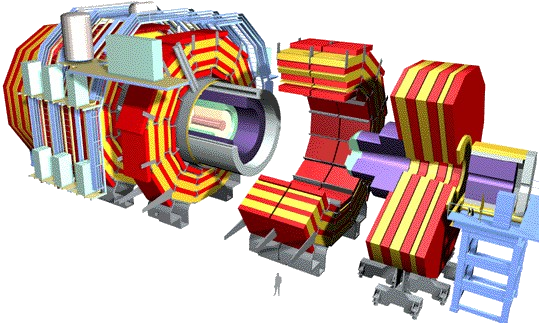
\includegraphics[width=\marginparwidth]{LHC/cms.png}
    \captionof{figure}{CMS.}
    	\label{cms}
}
\marginpar
{
	
	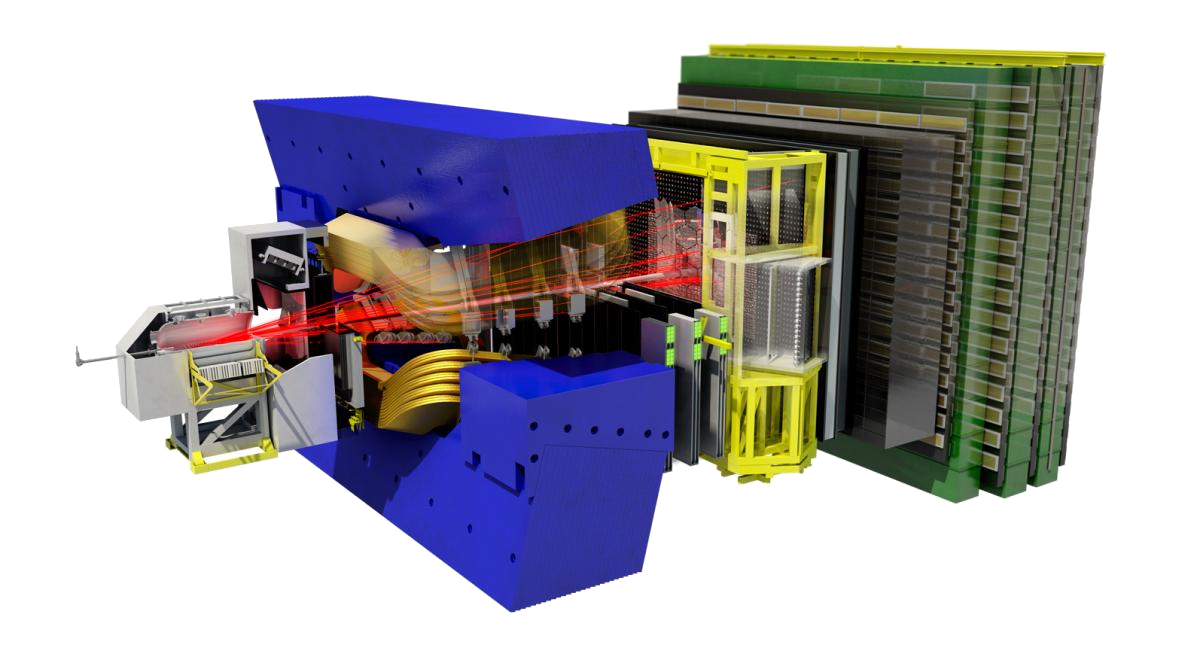
\includegraphics[width=\marginparwidth]{LHC/lhcb.png}
    \captionof{figure}{LHCb.}
    	\label{lhcb}
}

\section{Luminosité des faisceaux}
\chapter{Le détecteur Compact Muon Solenoid (CMS)}
\renewcommand\chapterillustration{CMS/cms.jpeg}
\ThisULCornerWallPaper{1}{\chapterillustration}
\minitoc

\lettrine[lines=4, slope=-0.5em]{C}{e} chapitre décrit le détecteur CMS et les sous-détecteurs qui le compose, suivi d'une discussion sur le système de déclenchement. Il décrit également certaines des mises à niveau qui se dérouleront durant les \textit{Long Shut Down} LS2 et LS3 afin de se préparer à l'augmentation de la luminosité et de l'empilement qui en découle.

\section{Le détecteur Solénoïde compact à muons (CMS)}
Le détecteur Solénoïde Compact à Muons abrégé en CMS (pour \textit{Compact Muon Solenoid}) est avec ATLAS une expérience généraliste qui a comme buts majeurs :

\begin{itemize}[label=$\bullet$]
	\item \textbf{La recherche du boson de Higgs : } Lors de la conception de CMS dans les années \num{1990}, la détection du boson de Higgs a été prise comme référence afin de tester les performances du design du détecteur. Ce but a été réalisé avec la découverte d'une particule compatible avec le boson de Higgs le \num{4} juillet \num{2012}.
	\item \textbf{Confirmer et préciser les mesures de la physique du Modèle Standard : } Des mesures de précisions dans des domaines tels que la QCD, le couplage électrofaible, et la physique des saveurs pourraient donner des indications d'une physique au-delà du Modèle Standard.
	\item \textbf{La recherche de signes de physique au-delà du Modèle Standard : }CMS permet la recherche de particules supersymétriques ou de nouveaux bosons vecteurs massifs ($Z'$) ou encore la recherche de dimensions supplémentaires par exemple.
	\item \textbf{Étudier les collisions d'ions lourds.}
\end{itemize}

Afin de répondre à ces objectifs, le "\textit{Technical Design Report}" (TDR) \cite{Bayatian:922757} a fixé le cahier des charges et les caractéristiques essentielles du détecteur CMS, à savoir :
\begin{itemize}[label=$\bullet$]
	\item Une bonne identification des muons et une bonne résolution en impulsion sur une vaste gamme d'impulsion pour la région $|\eta|<$\num{2.5}, une bonne résolution en masse pour les dimuons ($\approx$ \num{1}\% à \SI{100}{\giga\eV/\square\c}) et la capacité à déterminer de manière certaine la charge des muons d'impulsion $p<$ \SI{1}{\tera\eV/\c}.
	\item Une bonne résolution en impulsion pour les particules chargées ainsi qu'une bonne efficacité de reconstruction dans le trajectographe interne (\textit{inner tracker}). Un déclenchement et un étiquetage efficace pour les jets venant de quarks $\tau$ et $b$, ce qui requiert un détecteur à pixels proche du point d'interaction.
	\item Une bonne résolution pour l'énergie électromagnétique, et une bonne résolution en masse pour les diphotons et diélectrons  ($\approx$ \num{1}\% à \SI{100}{\giga\eV/\square\c}), une grande couverture géométrique ($|\eta|<2.5$), une mesure de la direction des photons et/ou une localisation correcte du vertex primaire d'interaction ainsi qu'une bon rejet des $\pi_{0}$ et une isolation des photons et leptons efficace à haute luminosité.
	\item une bonne résolution en masse des dijets et une bonne résolution en masse de l'énergie transverse manquante $E_{T}^{miss}$. Ceci requiert un calorimètre hadronique hermétique de très grande couverture géométrique ($|\eta|<5$) et une fine segmentation latérale ($\Delta\eta\times\Delta\phi<0.1\times0.1$)
\end{itemize} 

\subsection{Systèmes de coordonnées conventionnels}
Le système de coordonnées utilisé dans CMS est un repère cartésien $\left(O,\vec{x},\vec{y},\vec{z}\right)$ où $O$ est l'origine du repère et coïncide avec le point nominal d'interaction (IP) qui est le centre du détecteur. Le système de coordonnées est déterminé par l'axe $z$ qui est défini comme étant parallèle et dans la même direction que le faisceau allant dans le sens anti-horaire vue de dessus. L'axe $x$ pointe vers le centre du collisionneur LHC. L'axe $y$ est orthogonal au plan $xz$ et pointe vers le haut. CMS possédant une symétrie cylindrique, le repère $\left(O,\vec{r},\vec{\phi},\vec{z}\right)$ est souvent utilisé. $z$ correspond à la distance entre le plan perpendiculaire à l'axe du faisceau (appelé plan transverse) passant par le point considéré et l'origine $O$ du repère; $\phi$ est mesuré par rapport à l'axe $\vec{x}$ dans le plan $xy$ (angle d'émission par rapport à l'axe du faisceau) et $r=\sqrt{x^2+y^2}$. L'angle polaire $\theta$ est définit par rapport à $z$. Un troisième type de coordonnées, utilisant le fait que les particules produites au LHC sont relativistes, est également utilisé. En décomposant l'impulsion de la particule en une composante transverse et longitudinale $p=p_{T}+p_{L}=\sqrt{p_{x}^{2}+p_{y}^{2}}+p_{z}$ :
\begin{equation}
(E/c)^{2}=(mc)^{2}+p_{T}^{2}+p_{L}^{2}\Longrightarrow (E/c)^{2}-p_{L}^{2}=(mc)^{2}+p_{T}^{2}\Longrightarrow  \begin{cases}
\left(E/c \right)=\sqrt{\left(mc \right)^{2}+p_{T}^{2}}\cosh(y) \\
p_{L}=\sqrt{\left(mc \right)^{2}+p_{T}^{2}}\sinh(y)
\end{cases}
\end{equation}
%qu'il est possible de réécrire comme :
%\begin{equation}
%\left(E/c \right)=\sqrt{\left(mc \right)^{2}+p_{T}^{2}}\cosh(y), p_{L}=\sqrt{\left(mc \right)^{2}+p_{T}^{2}}\sinh(y)
%\end{equation}
avec $y$ un paramètre appelé rapidité. En remarquant que $p_{l}=p_{z}=p\cos(\theta)$ et en faisant le développement de $E=\sqrt{m^{2}c^{4}+p^{2}c^{2}}$:
\begin{equation}
y=\arctan\left(\frac{p_{l}c}{E}\right)=\frac{1}{2}\log\left(\frac{E+p_{l}c}{E-p_{l}c}\right)=\frac{1}{2}\log\left(\frac{\cos^2 \theta/2+\cdots}{\sin^2 \theta/2+\cdots}\right)\backsimeq-\log\tan\left(\frac{\theta}{2}\right)=\eta
\end{equation}
%en remarquant que $p_{l}=p_{z}=p\cos(\theta)$ et en faisant le développement de $E=\sqrt{m^{2}c^{4}+p^{2}c^{2}}$
%\begin{equation}
%y=\frac{1}{2} \log\left(\frac{E+p_{l}c}{E-p_{l}c}\right)=\frac{1}{2}\log\left(\frac{\cos^2 %\theta/2+m^{2}c^{2}/4p^{2}+\cdots}{\sin^2 %\theta/2+m^{2}c^{2}/4p^{2}+\cdots}\right)\backsimeq-\log\tan\left(\frac{\theta}{2}\right)=\eta
%\end{equation}
$\eta$ est appelé pseudo-rapidité. On utilise donc le repère $\left(O,\vec{r},\vec{\eta},\vec{\phi}\right)$ pour décrire la géométrie de CMS.

\subsection{Description générale de CMS}
Le détecteur CMS se trouve dans une caverne située au point \num{5} (P5) du LHC, proche du village de Cessy en France. La construction de CMS s'est effectuée en surface et par tranches autonomes afin de réduire le temps et les coûts nécessaires à sa construction.
\marginpar
{
	\centering
	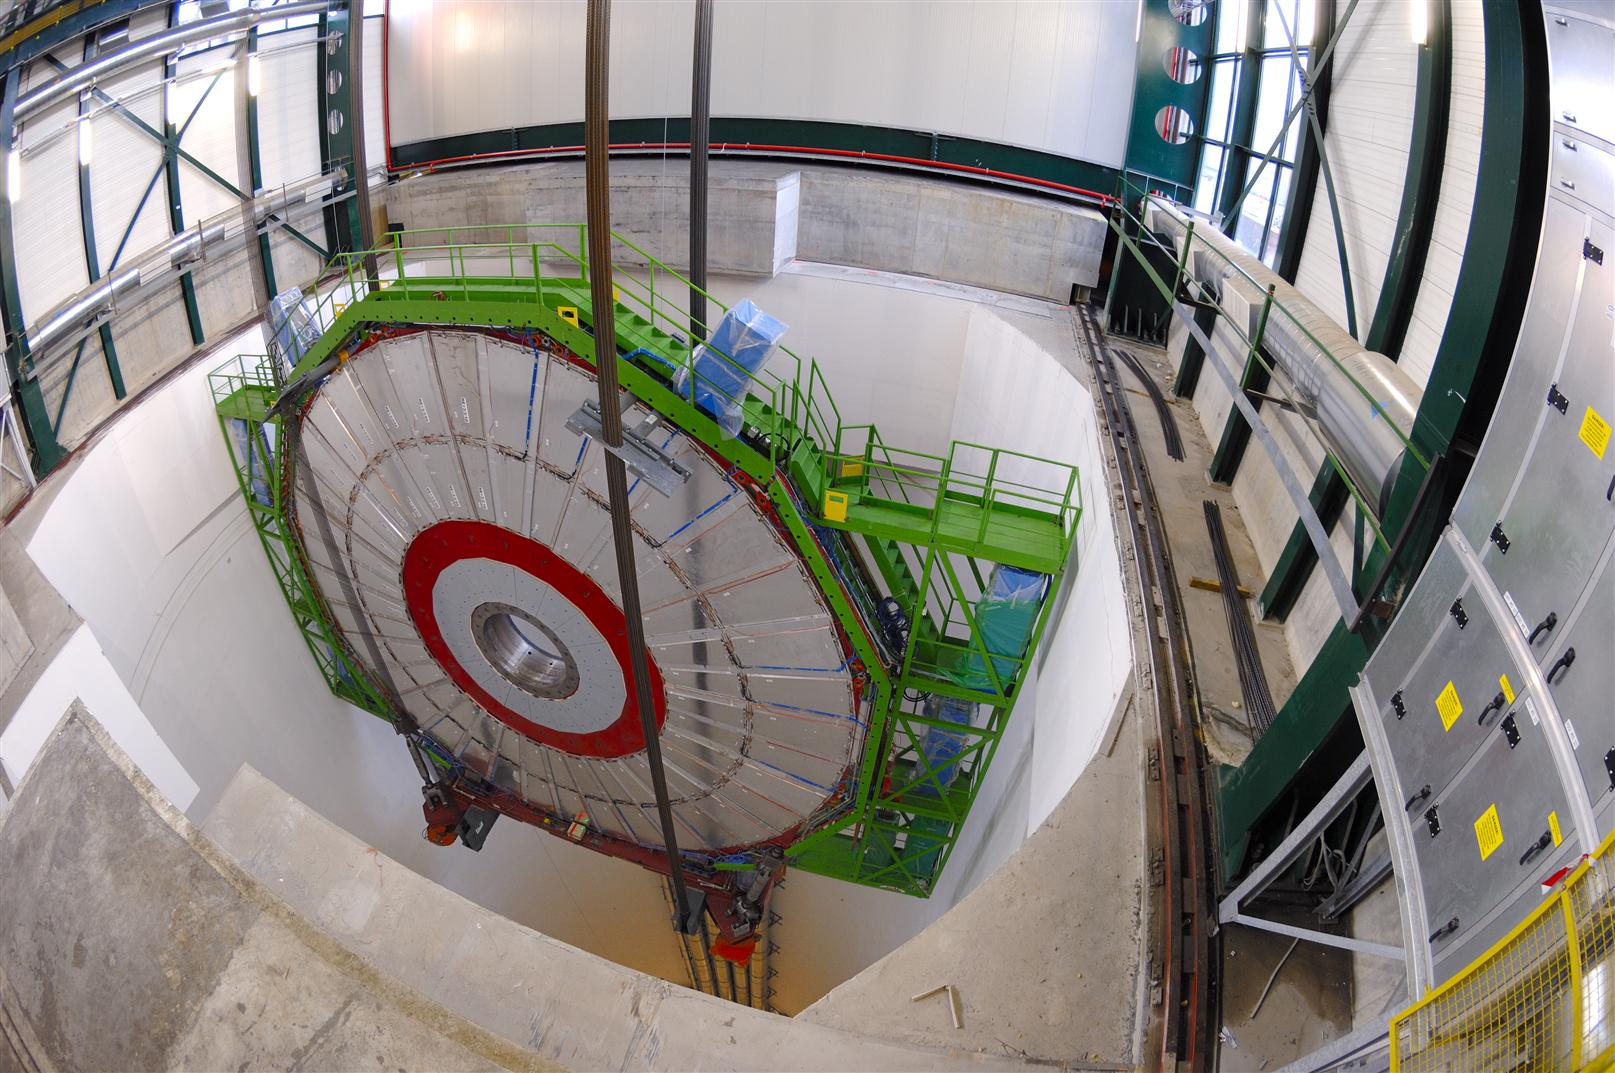
\includegraphics[width=\marginparwidth]{CMS/slice.jpg}
	\captionof{figure}{Descente d'une tranche de CMS.}
	\label{slice}
}
Chaque tranche à ensuite été descendue dans la caverne et assemblée à \SI{100}{\meter} sous terre (cf.Fig~\ref{slice}).
CMS est une détecteur cylindrique de \SI{24}{\meter} de long et de \SI{14.6}{\meter} de diamètre pour une masse de plus de \num{16000} tonnes (cf.Fig~\ref{cmsexploded}). Il est composé d'une succession de sous-détecteurs concentriques.

\begin{sidewaysfigure}
	\centering
	\includegraphics[width=0.80\textwidth]{CMS/cms.png}
	\caption{\label{cmsexploded}Vue éclatée du détecteur CMS.}
\end{sidewaysfigure}
\newpage
En partant du centre vers l'extérieur :
\begin{itemize}[label=$\bullet$]
	\item \textbf{Le trajectographe : } C'est le sous-détecteur le plus proche du point d'interaction. Il permet de reconstruire la trajectoires des particules chargées.
	 \item \textbf{Le calorimètre électromagnétique (ECAL\footnote{Pour \textit{Electromagnetic CALorimeter}.})}: Il permet de mesurer l'énergie des photons et des électrons.
	 \item \textbf{Le calorimètre hadronique (HCAL\footnote{Pour \textit{Hadronic CALorimeter}.})}: Il permet de mesurer l'énergie des hadrons.
	 \item \textbf{L'aimant supra-conducteur : } Il produit un champ de \SI{3.8}{\tesla} et permet de courber la trajectoire des particules chargées.
	 \item \textbf{Les chambres à muons : } Elles permettent d'identifier, reconstruire la trajectoire et mesurer l'énergie des muons. 
\end{itemize}
Chaque composant de CMS fera l'objet d'une description plus détaillée dans les paragraphes suivants.

\section{Les sous-détecteurs de CMS}
\subsection{Le trajectographe}
Le trajectographe de CMS (cf.Fig~\ref{trajectographe}) est le détecteur le plus proche du faisceau et du point de collision. Le trajectographe est composé de deux sous-détecteurs : le détecteur à pixels et le trajectographe à micro-pistes de silicium. Il a pour but de reconstruire les traces des particules chargées issues des collisions grâce à des suites d'impacts enregistrés par les couches du détecteur. La trace reconstruite permet de déterminer la charge et l'impulsion de la particule associée. En effet, une particule de charge $q$ qui se déplace dans un champ magnétique subit une force donné par la formule de \bsc{Lorentz}. La trajectoire de la particule dans le cas d'un champ magnétique d'intensité $B$ est hélicoïdale, de rayon $R_{c}$. Il est ainsi possible dans déduire l'impulsion transverse :
\begin{equation}
p_{T}=qBR_{c}
\end{equation}
En prenant les positions selon $r$ des hits, il est possible d'en déduire l'angle $\theta$, angle entre la trajectoire de la particule est le faisceau et donc de calculer l'impulsion totale:
\begin{equation}
p=\frac{p_{T}}{\sin\theta}
\end{equation}
\begin{figure}[ht!]
	\centering
	\includegraphics[width=0.65\textwidth]{CMS/tracker.png}
	\captionof{figure}{Schéma du trajectographe de CMS. Chaque trait représente un module du détecteur. Les lignes doubles correspondent à des modules mis dos à dos produisant des hits dit "stéréos". Le détecteur à pistes est composé de quatre sous-détecteurs : Les tonneaux internes (TIB), les tonneaux externes (TOB), les disques internes (TID) et les bouchons (TEC).}
	\label{trajectographe}
\end{figure}

\subsubsection{Le détecteur à pixels}
Le détecteur à pixels de CMS a récemment été remplacé afin de garder une trajectographie performante à des luminosités au dessus de \SI{2e34}{\per\square\centi\meter\per\second} et avec un empilement de plus de \num{50}. Ce remplacement a eu lieu du \num{28} février au \num{7} mars \num{2017} durant l'arrêt technique hivernal prolongé (EYETS). Le nouveau détecteur à pixels se compose d'un tonneau constitué de quatre couches de détection (BPIX) à des distances du faisceau $r=\SI{3.0}{\centi\meter}$, \SI{6.8}{\centi\meter}, \SI{10.2}{\centi\meter} et \SI{16}{\centi\meter} et d'une longueur de \SI{548.8}{\milli\meter} et de trois bouchons (FPIX) situé à $\pm$\SI{29.1}{\centi\meter}, $\pm$\SI{39.6}{\centi\meter} et $\pm$\SI{51.6}{\centi\meter} pour une couverture radiale allant de \num{4.5} à \SI{16.1}{\centi\meter}. Une comparaison entre l'ancien détecteur à pixel et le nouveau est donnée figure \ref{pixel}.

	\begin{figure}[ht!]
	\subfloat[Vue oblique-transverse comparant les couches des tonneaux de l'ancien (gauche) et du nouveau détecteur (droite).]{\includegraphics[width=.45\linewidth]{CMS/pixel.png}}
	\hfill
	\subfloat[Ancien détecteur à pixel (bas) et nouveau (haut).]{\includegraphics[width=.45\linewidth]{CMS/pixel2.png}}
	\caption{Comparaison entre le nouveau et l'ancien trajectographe à pixels.}
	\label{pixel}
\end{figure}

L'ajout d'une quatrième couche de détection dans le barrel assure une redondance lors de la reconnaissance de motifs et permet de réduire le taux d'erreurs lors d'empilement importants. Il assure également une sécurité au cas où la couche la plus proche du point d'interaction viendrait à se détériorer plus vite que prévu. Cependant, elle augmente le budget matière du détecteur, il a donc été nécessaire de repenser le support et les services afin d'être plus léger. Un nouveau système de refroidissement au \chemform{CO_2} ainsi que le déplacement des systèmes passifs (connectique, plaques d'électronique) hors du volume de trajectographie ont également été effectués (cf.Fig~\ref{pixel2}).

\begin{figure}[ht!]
	\centering
	\includegraphics[width=0.75\textwidth]{CMS/pixel3.png}
	\captionof{figure}{Vue explosée du nouveau détecteur à pixels. La figure montre les positions des différentes partitions FPIX et BPIX ainsi que leurs cylindres contenant leurs services respectifs. Les services nécessaires au détecteur (connectiques, fibres optiques, convertisseurs DC-DC sont situés à haut $\eta$, hors du volume de trajectographie).}
	\label{pixel2}
\end{figure}

Ce détecteur contient plus de \num{97} millions de pixels (\num{79} pour les BPIX et \num{18} pour les FPIX) mesurant \num{100}$\times$\SI{150}{\square\micro\meter} de section et \SI{250}{\micro\meter} d'épaisseur. Ces pixels sont regroupés en modules (\num{1184} pour BPIX et \num{672} pour FPIX) (cf.Fig~\ref{module}) de \num{66560} pixels  (\num{8}$\times$\num{2} ROCs) d'une épaisseur de \SI{75}{\micro\meter} pour la première couche du BPIX et \SI{250}{\micro\meter} pour le reste du BPIX et FPIX.

	\begin{figure}[ht!]
	\centering
	\subfloat[Module pour les couches \num{2} à \num{4} des BPIX et des FPIX (gauche) et de la couche \num{1} de BPIX (droite).]{\includegraphics[width=.46\linewidth]{CMS/module.png}}
	\hfill
	\subfloat[Schéma de l'électronique de lecture d'un module.]{\includegraphics[width=.46\linewidth]{CMS/module2.png}}
	\caption{Modules de pixels.}
	\label{module}
\end{figure}
\subsubsection{Le détecteur à pistes}
Le détecteur à pistes mesure \SI{5.5}{\meter} de long pour \SI{2.4}{\meter} de diamètre pour une aire active de \SI{198}{\square\meter} et est le plus grand détecteur au silicium jamais construit. Il comporte en tout \num{15148} modules pour un total de \num{9.3} millions de pistes lues par \num{76000} puces électroniques. Il peut être décomposé en quatre sous-détecteurs :

\begin{itemize}[label=$\bullet$]
\item \textbf{Le tonneau interne} (TIB) (cf.Fig~\ref{TIB}) pour  \textit{Tracker Inner Barrel} est composé de \num{2724} modules répartis en quatre couches. Chaque couche se compose de pistes de silicium d'une épaisseur de \SI{320}{\micro\meter} avec un pas de \SI{80}{\micro\meter} pour les deux premières couches et de \SI{120}{\micro\meter} pour les deux dernières. Elles sont orientées parallèlement au faisceau. Les deux premières couches sont composées de modules dits "stéréos" qui sont la juxtaposition de deux modules collés l'un l'autre avec un angle de \SI{100}{\milli\radian} entre les deux, ce qui permet d'avoir une résolution de \num{23} à \SI{34}{\micro\m} dans le plan transverse et de \SI{230}{\micro\meter} dans le plan longitudinal. Son rayon est compris entre \num{25} et \SI{52}{\centi\meter} et sa longueur couvre le domaine $|z|<$\SI{65}{\centi\meter}.

\item \textbf{Les disques internes} (TID) (cf.Fig~\ref{TID}) pour \textit{Tracker Inner Disk} sont composés de trois disques parallèles qui sont compris dans le domaine \SI{75}{\centi\meter}$<|z|<$\SI{110}{\centi\meter}. Chaque disque est composé de trois anneaux concentriques. Les \num{816} modules sont composés de strips d'une épaisseur de \SI{320}{\micro\meter} orientés radialement pour un pas compris entre \SI{81} et \SI{158}{\micro\meter}. Comme pour le TIB, les deux premiers modules sont "stéréos".
\marginpar
{
	\centering
	\includegraphics[width=\marginparwidth]{CMS/TOB_TEC.png}
	\captionof{figure}{Différents modules utilisés pour la construction du TOB et du TEC.}
	\label{TOB_TEC}
}
\item \textbf{Le tonneau externe } (TOB) (cf.Fig~\ref{TOB}) pour \textit{Tracker Outer Barrel} entoure les TIB et TID pour couvrir un espace entre \num{60} et \SI{100}{\centi\meter} en rayon et $|z|<$\SI{110}{\centi\meter}. Il est composé de \num{5208} modules (cf.Fig~\ref{TOB_TEC}) de pistes orientées parallèlement aux faisceaux et de pas compris entre \num{122} et \SI{183}{\micro\meter}. Ces modules sont répartis en six couches dont les deux dernières sont "stéréos". L'épaisseur de ces modules est de \SI{500}{\micro\meter}.   

\item \textbf{Les bouchons }(TEC) (cf.Fig~\ref{TEC}) pour \textit{Tracker End-Cap} sont composés de neuf disques chacun, de \num{4} à \num{7} anneaux concentriques. Ils couvrent \num{25}--\SI{110}{\centi\meter} en rayons et \num{120}--\SI{275}{\centi\meter} en $|z|$. Les deux premiers disques ainsi que le cinquième sont "stéréos". Les trois premiers anneaux sont composés de \num{1256} modules par bouchon (cf.Fig~\ref{TOB_TEC}) d'épaisseur \SI{320}{\micro\meter} et de pas inter-pistes compris entre \num{81} et \SI{158}{\micro\meter}. Les quatre anneaux suivant, sont composés de \num{1944} modules par bouchon (cf.Fig~\ref{TOB_TEC}), d'épaisseur \SI{500}{\micro\meter} de pas inter-strip \num{113}--\SI{172}{\micro\meter}.
\end{itemize}

	\begin{figure}[ht!]
	\centering
	\subfloat[Le TIB.]{\includegraphics[width=.40\linewidth]{CMS/TIB.jpg}\label{TIB}}
	\subfloat[Un TID.]{\includegraphics[width=.40\linewidth]{CMS/TID.jpg}\label{TID}}
	\\
	\subfloat[Le TOB.]{\includegraphics[width=.40\linewidth]{CMS/TOB.jpg}\label{TOB}}
	\subfloat[Un TEC.]{\includegraphics[width=.40\linewidth]{CMS/TEC.jpg}\label{TEC}}
	\caption{Photos des différents composants du détecteur à pistes.}
\end{figure}

\newpage
\subsection{Le calorimètre électromagnétique}
Le calorimètre électromagnétique de CMS ou \textit{Electromagnetic CALorimeter} (ECAL), permet de mesurer l'énergie et la direction des particules réagissant principalement à l'interaction électromagnétique. Ce sont surtout les photons et les électrons qui seront détectés; ils perdent leur énergie par des processus radiatifs. La distance caractéristique est donnée par la longueur de radiation $X_{0}$, dépendante du matériau, définie comme le libre parcours moyen pour le processus de radiation. Des photons de \SI{100}{\giga\eV} perdent à peu près toute leur énergie dans \num{20}$\times X_{0}$.
\begin{figure}[ht!]
	\centering
	\includegraphics[width=0.90\textwidth]{CMS/ECAL.png}
	\captionof{figure}{Schéma du ECAL de CMS.}
	\label{ECAL}
\end{figure}

Le calorimètre électromagnétique est composé de \num{75848} cristaux (cf.Fig~\ref{crystaux}) de \chemform{PbWO_4} (\SI{11}{\cubic\meter}, \num{92} tonnes) et peut se décomposer en trois sous-structures (cf.Fig~\ref{ECAL}) :
\begin{itemize}[label=$\bullet$]
	\item \textbf{Le tonneau} ou EB (cf.Fig~\ref{EB}) pour \textit{Electromagnetic Barrel} contient \num{61200} cristaux de tungstate de plomb. Le tonneau est divisé en \num{36} supermodules couvrant chacun la moitié de la longueur du tonneau. Chaque super-module contient \num{1700} cristaux de \num{22}$\times$\SI{22}{\square\milli\meter} et de longueur \SI{230}{\milli\meter}. Les cristaux sont arrangés de manière à former \num{170}-$\eta$ anneaux contenant \num{360} cristaux chacun. Un cristal couvre environ \SI{1}{\degree} en $\phi$. Le tonneau couvre une zone en pseudorapidité de $|\eta|<$\num{1.479}. Les photodiodes à avalanche (cf.Fig~\ref{APD}) (APD) sont utilisées pour détecter la scintillation.
	\marginpar
	{
		\centering
		\includegraphics[width=\marginparwidth]{CMS/Crystaux.png}
		\captionof{figure}{Un cristal de \chemform{PbWO_4}.}
		\label{crystaux}
	}
	
	\marginpar
	{
		\centering
		\includegraphics[width=\marginparwidth]{CMS/APD.png}
		\captionof{figure}{Un groupe de deux APD.}
		\label{APD}
	}
	\marginpar
	{
		\centering
		\includegraphics[width=\marginparwidth]{CMS/dee.jpg}
		\captionof{figure}{Un \textit{"Dee"}.}
		\label{DEE}
	}
	\marginpar
	{
		\centering
		\includegraphics[width=\marginparwidth]{CMS/20SCs.jpg}
		\captionof{figure}{Montage de \num{20} Super-Cristaux sur un des \textit{Dee}.}
		\label{SP}
	}
	\marginpar
	{
		\centering
		\includegraphics[width=\marginparwidth]{CMS/VPT.png}
		\captionof{figure}{Une VPT.}
		\label{VPT}
	}
	
	\item \textbf{Les bouchons} (EE) (cf.Fig~\ref{EE}) pour \textit{Electromagnetic End-cap} sont perpendiculaires aux faisceaux et ferment le EB. Ils sont situés à \SI{315}{\centi\meter} du point d'interaction et couvrent une section en $\eta$ allant de \num{1.479} à \num{3}. Chaque bouchon se décompose en deux demi-disques appelés \textit{"Dee"} (cf.Fig~\ref{DEE}). Chaque \textit{Dee} est constitué de \num{3662} cristaux de \num{2.86}$\times$\SI{2.86}{\centi\meter} et de longueur \SI{220}{\milli\meter} regroupés en matrices de \num{5}$\times$\num{5} qu'on appelle Super-Cristaux (cf.Fig~\ref{SP}). La scintillation est détectée par des phototriodes à vide (VPT) (cf.Fig~\ref{VPT}). Les cristaux de \chemform{PbWO_4} ont une grande densité ($\rho=$\SI{8.28}{\gram\per\cubic\centi\meter}), une longueur d'interaction $X_{0}$ assez courte de \SI{0.89}{\centi\meter} est un petit rayon de Molière ($r_{M}=$\SI{2.2}{\centi\meter}) ainsi qu'une grande vitesse de radiation (\num{80}\% dans \SI{25}{\nano\second}). 
	\item \textbf{L'initiateur de gerbe } (cf.Fig~\ref{PRESHOWER}), appelé \textit{Preshower} est placé entre le EB et le EE. Il consiste en deux couches de détecteurs de silicium de pas \SI{1.9}{\milli\meter} intercalées entre deux couches en plomb (\num{2}$X_{0}$ devant et \num{1}$X_{0}$ derrière la première couche de silicium). Il permet d'améliorer la précision de la mesure de la position de la gerbe électromagnétique et la discrimination $\gamma/\pi_{0}$. Il couvre une région comprise entre \num{1.653}$<|\eta|<$\num{2.6}.
\end{itemize}
\begin{figure}[ht!]
	\centering
	\subfloat[Le tonneau du ECAL (EB).]{\includegraphics[width=0.8\linewidth]{CMS/EB.jpg}\label{EB}}
	\\
	\subfloat[Un bouchon du ECAL (EE).]{\includegraphics[width=.40\linewidth]{CMS/EE.jpg}\label{EE}}
	\subfloat[Un des preshower du ECAL.]{\includegraphics[width=.40\linewidth]{CMS/preshower.jpg}\label{PRESHOWER}}
	\caption{Photos des différents composants du calorimètre électromagnétique.}
\end{figure}
\subsection{Le calorimètre hadronique}
	\marginpar
{
	\centering
	\includegraphics[width=\marginparwidth]{CMS/LAITON.jpg}
	\captionof{figure}{Photo de douilles de la marine russe réutilisées pour la construction du HCAL.}
	\label{LAITON}
}
	\marginpar
{
	\centering
	\includegraphics[width=\marginparwidth]{CMS/SCINTI.png}
	\captionof{figure}{Photo d'une tuile du HO avec des fibres WLS insérées dans les \num{4} $\sigma$-rainures.}
	\label{SCINTI}
}
\marginpar
{
	\centering
	\includegraphics[width=\marginparwidth]{CMS/MPPC.png}
	\captionof{figure}{Photo d'un MPPC.}
	\label{MPPC}
}
\marginpar
{
	\centering
	\includegraphics[width=\marginparwidth]{CMS/HPD.png}
	\captionof{figure}{Photo d'une HPD.}
	\label{HPD}
}
Le calorimètre hadronique de CMS ou \textit{Hadronic CALorimeter} (HCAL) (cf.Fig~\ref{HCAL}) permet de mesurer l'énergie et la direction des hadrons issus de l'hadronisation des quarks et gluons produits lors des collisions. Ce détecteur à une grande compacité spatiale et énergétique et est très compact car il se trouve pour une grande partie entre le ECAL et l'aimant supraconducteur. Cette disposition a nécessité de maximiser la quantité d'absorbeur et de minimiser les parties actives du détecteur. L'absorbeur est constitué de laiton (cf.Fig~\ref{LAITON}) qui possède une faible longueur d'interaction $\lambda_{l}$ et un faible taux de diffusions multiples. Les hadrons perdent majoritairement leur énergie par interaction nucléaire avec l'absorbeur. La plupart des hadrons sont stoppés avec \num{9}$\lambda_{l}$. Le laiton est également non magnétique ce qui est nécessaire vu l'emplacement du calorimètre. Le matériau actif est composé de feuilles de scintillateurs fluorescents (cf.Fig~\ref{SCINTI}). La scintillation est ensuite récoltée par des fibres optiques qui décalent la longueur d'onde de la lumière (WLS). Le signal est ensuite lu par des \textit{Multi-Pixel Photon Counter} (MPPC) (cf.Fig~\ref{MPPC}) pour le sous-détecteur \textit{Hadronic Outward calorimeter} et par des photodiodes hybrides (HPD) (cf.Fig~\ref{HPD}) pour les autres sous-détecteurs.
\begin{figure}[ht!]
	\centering
	\includegraphics[width=0.95\textwidth]{CMS/HCALSCHEME.png}
	\captionof{figure}{Schéma d'un quart d'une coupe du HCAL de CMS.}
	\label{HCAL}
\end{figure}

Le calorimètre hadronique couvre une zone en pseudo-rapidité jusqu'à $|\eta|<$\num{5.0}. Il possède plus de \num{70000} feuilles de scintillateurs. Il est composé de \num{4} sous-détecteurs subdivisés en tours : 
\begin{itemize}[label=$\bullet$]
	\item \textbf{Le tonneau} HB pour \textit{Hadronic Barrel calorimeter} (cf.Fig~\ref{HB}) couvre la région en pseudo rapidité $|\eta|<1.3$. Il est constitué de \num{36} quartiers couvrant \SI{20}{\degree} en $\phi$ découpés en quatre sous secteurs de \SI{5}{\degree} en $\phi$ et \num{16} sous secteurs en $\eta$. Un quartier possède \num{16} couches qui sont des empilements de scintillateurs de \SI{9}{\milli\meter} d'épaisseur pour les couches les plus externes et \SI{3.7}{\milli\meter} pour les autres et d'absorbeur de (\SI{40}{\milli\meter} de fer pour la première couche, \SI{50.5}{\milli\meter} de laiton pour les huit suivantes, \SI{56.5}{\milli\meter} de laiton pour les six suivantes et \SI{75}{\milli\meter} de fer pour la dernière). Les tours ont une segmentation de $\Delta\eta\times\Delta\phi=$\num{0.087}$\times$\num{0.087}.
	\item \textbf{Les deux bouchons} HE pour \textit{Hadronic End-cap calorimeter} (cf.Fig~\ref{HE}) couvrent les régions comprises entre $|\eta|>$\num{1.3} et $|\eta|<$\num{3.0}. Une zone inclinée à \SI{53}{\degree} par rapport à l'axe du faisceau et ne pointant pas vers le point d'interaction est laissée libre afin de permettre le passage des câbles et systèmes nécessaires au trajectographe et au calorimètre électromagnétique. Les bouchons sont segmentés en \num{18} quartiers de \SI{20}{\degree} en $\phi$ chacun composé de \num{14} tours en $\eta$. Les tours sont des empilements de scintillateurs de \SI{3.7}{\milli\meter} d'épaisseur et d'une couche d'absorbeur (\SI{9}{\milli\meter} pour la première couche et \SI{7.5}{\milli\meter} pour les suivantes). Une tour possède \num{19} couches de  scintillateurs en tout. Les \num{5} tours couvrant $|\eta|<$\num{1.74} ont une segmentation de $\Delta\eta\times\Delta\phi=$\num{0.087}$\times$\num{0.087} alors que les \num{8} couvrant \num{1.74}$<|\eta|<$\num{3.0} ont des segmentations allant de $\Delta\eta\times\Delta\phi=$\num{0.09}$\times$\num{0.174} à $\Delta\eta\times\Delta\phi=$\num{0.35}$\times$\num{0.174}.
	\item \textbf{Le calorimètre externe} HO pour \textit{Hadronic Outward calorimeter} (cf.Fig~\ref{HO}) est placé à l'extérieur de l'aimant supraconducteur. Il est constitué de couches de scintillateurs de \SI{10}{\milli\meter} d'épaisseur et couvre la région $|\eta|<$\num{1.26}. Ce sous-détecteur permet de récupérer l'énergie sortant du HB et assure une longueur d'interaction de plus de \num{10}$\lambda_{l}$. Le HO est composé de \num{5} anneaux de \SI{2.536}{\meter} de long selon $z$ numérotés $-$\num{2}, $-$\num{1}, \num{0}, $+$\num{1}, $+$\num{2} et de centre $z=-$\num{5.324}, \num{2.686}, \num{0}, \num{2.686} et \SI{5.324}{\meter} respectivement. Le premier anneau est composé de deux couches de scintillateurs de \SI{10}{\milli\meter} d'épaisseur placées en $r=$\SI{3.82}{\meter} et \SI{4.07}{\meter}. Les autres anneaux ne possèdent qu'une couche de scintillateur placé à $r=$\SI{4.07}{\meter}. Chaque anneau est segmenté en \num{12} secteurs en $\phi$. Chaque secteur est segmenté en \num{8}, \num{6} et \num{5} tuiles de scintillateurs (cf.Fig~\ref{SCINTI}) pour les anneaux \num{0}, $\pm$\num{1}, $\pm$\num{2} respectivement.
	\item \textbf{Les calorimètres très à l'avant} HF pour \textit{Hadronic Forward calorimeter} couvrent une zone en pseudo-rapidité comprise entre $|\eta|>$\num{3.0} et $|\eta|<$\num{5.0} et \SI{12.5}{\centi\meter}$<r<$\SI{130}{\centi\meter}. Ils sont situés à une distance $|z|=$\SI{11.2}{\meter} et font \SI{1.65}{\meter} de long. Ils consistent en un absorbeur de fer qui intègre des fibres de quarks résistantes aux radiations qui assurent la collection rapide de la lumière \bsc{Čerenkov}. La moitié de ces fibres font toute la longueur du détecteur (\SI{1.65}{\meter}) alors que d'autres commencent à \SI{22}{\centi\meter} (soit \SI{143}{\centi\meter} de long) du bord placées vers l'intérieur de CMS. Elles sont placées alternativement à une distance de \SI{5}{\milli\meter} l'une de l'autre en $r$  avec segmentation de $\Delta\eta\times\Delta\phi=$\num{0.175}$\times$\num{0.175}. Cette différence de longueur permet de séparer les cascades électromagnétiques des cascades hadroniques. La lumière est ensuite collectée par des tubes photo-multiplicateurs (PMT). Le HF est composé de \num{18} secteurs de \SI{20}{\degree} en $\phi$. Chaque secteur comporte \num{13} anneaux en $\eta$.
\end{itemize}
\begin{figure}[ht!]
\centering
\subfloat[Le tonneau du HCAL (HB).]{\includegraphics[width=.40\linewidth]{CMS/HB.jpg}\label{HB}}
\subfloat[Un bouchon du HCAL (HE).]{\includegraphics[width=.40\linewidth]{CMS/HE.jpg}\label{HE}}
\\
\subfloat[Installation du HO.]{\includegraphics[width=.40\linewidth]{CMS/HO.jpg}\label{HO}}
%http://cms.desy.de/e53612/e155171/e155181/
\subfloat[Un des HF du HCAL.]{\includegraphics[width=.40\linewidth]{CMS/HF.jpg}\label{HF}}
\caption{Photos des différents composants du calorimètre hadronique.}
\end{figure}
\vspace*{-0.3cm}	
\subsection{L'aimant supraconducteur}
\vspace*{-0.3cm}
L'aimant supraconducteur de CMS (cf.Fig~\ref{MAGNET}) est un solénoïde de \SI{5.9}{\meter} de diamètre pour \SI{12.9}{\meter} de longueur qui a été prévu pour créer un champ magnétique de \SI{4}{\tesla} à un courant de \SI{19.14}{\kilo\ampere}. À pleine puissance, il stocke une énergie de \SI{2.7}{\giga\joule}. Il est composé de \num{5} bobines en nobium-titane composées de \num{2168} spires, refroidies à une température de \SI{4.2}{\kelvin} par de l'hélium liquide. Une structure de retour de champ en fer de \num{11500} tonnes, composée de \num{5} culasses (cf.Fig~\ref{CULASSE}) et \num{2} bouchons, chacun composé de \num{3} disques, l'entoure et sert de structure de maintien des chambres à muons. L'épaisseur totale du retour est d'environ \SI{1.5}{\meter} (l'épaisseur du troisième disque des bouchons et du premier anneau du tonneau est de \SI{30}{\centi\meter}) et les autres disques des bouchons ainsi que les deuxième et troisième anneaux du tonneau font \SI{60}{\centi\meter}. L'épaisseur à été étudiée afin d'être suffisante pour absorber les hadrons qui traverseraient les calorimètres et l'aimant tout en restant assez fin pour éviter les pertes radiatives pour les muons.
\marginpar
{
	\centering
	\includegraphics[width=\marginparwidth]{CMS/CULASSE.jpg}
	\captionof{figure}{Photo d'une culasse.}
	\label{CULASSE}
}
\begin{figure}[ht!]
	\centering
	\includegraphics[width=0.50\textwidth]{CMS/MAGNET.png}
	\captionof{figure}{Schéma de l'aimant supra-conducteur de CMS.}
	\label{MAGNET}
\end{figure}
\newpage
La figure \ref{CHAMP} montre une simulation par éléments-finis de la valeur du champ magnétique en fonction de la position.
\begin{figure}[ht!]
	\centering
	\includegraphics[width=0.90\textwidth]{CMS/CHAMP.png}
	\captionof{figure}{Valeur du champ magnétique (gauche) et lignes de champ (droite) selon une coupe longitudinale du détecteur CMS, prédits par la simulation. Pour une valeur du champ central de \SI{3.8}{\tesla}.}
	\label{CHAMP}
\end{figure}
\subsection{Le spectrographe à muons}
\label{RPCPRE}
Le spectographe à muons (cf.Fig~\ref{CMS1}, Fig.~\ref{CMS2}) a pour but d'identifier les muons, de mesurer avec précision leur quantité de mouvement et de déclencher sur les événements contenant des muons.
\marginpar
{
	\centering
	\includegraphics[width=\marginparwidth]{CMS/MUON.png}
	\captionof{figure}{Quart d'une coupe dans le plan transverse du détecteur CMS montrant la trajectoire d'un muon (courbe bleue).}
	\label{MUON}
} Les muons ont un très grand pouvoir de pénétration. Il est donc possible d'utiliser à la fois les traces chargées laissées dans le trajectographe et dans des détecteurs placés après l'aimant pour les identifier et les reconstruire de manière précise. Une bonne résolution de la quantité de mouvement des muons et leur bonne identification est obtenue grâce au champ magnétique intense de l'aimant et du retour de champ dans la culasse qui assure une trajectoire avec une double courbure. Cette culasse doit contenir des détecteurs de grande taille afin d'augmenter la probabilité de détection. Ils faut donc qu'ils soient peu onéreux et fiables. Il faut également que ces détecteurs ne soient pas atteints par d'autres particules afin d'assurer un signal propre, pour ce faire la distance depuis l'aimant jusqu'à la dernière station du spectrographe et de l'ordre de \num{16} longueurs de radiation, ce qui évite le bruit de fond hadronique résiduel venant du faisceau.

\begin{sidewaysfigure}
\centering
\includegraphics[width=0.80\textwidth]{CMS/CMSLONG.png}
\captionof{figure}{Coupe longitudinale d'un quart de CMS.}
\label{CMS1}
\end{sidewaysfigure}


\begin{figure}[p]
\centering
\includegraphics[width=0.98\textwidth]{CMS/CMSTRANS.png}
\captionof{figure}{Coupe transversale de la partie centrale CMS.}
\label{CMS2}
\end{figure}

Le spectrographe à muons, est composé de \num{3} sous-détecteurs :
\begin{itemize}[label=$\bullet$]
	\item \textbf{Les chambres à dérive} DT pour \textit{Drift Tube} (cf.Fig~\ref{DT}) sont présentes seulement dans le tonneau où le flux de muons est faible tout comme le bruit de fond des neutrons. Le champ magnétique est également assez faible ($\sim$\SI{0.4}{\tesla}) et uniforme. Ce détecteur est constitué de \num{250} chambres insérées dans la culasse de CMS. Elles sont disposées en quatre couches selon $r$ à des distances $r=$\num{4.0}, \num{4.9}, \num{5.9} et \SI{7.0}{\meter}. La culasse est composée selon l'axe $z$ de \num{5} roues numérotées de $-$\num{2} à \num{2}, chacune comportant \num{12} (sauf pour MB4 qui en possède \num{14} (cf.Fig~\ref{CMS2})) secteurs dans le plan transverse numérotés à partir de $\phi=$\num{0} et couvrant \SI{30}{\degree}. Ce détecteur couvre une zone en pseudo rapidité $|\eta|<$\num{1.2}. Chaque chambre est constituée de \num{8} couches de tubes (cf.Fig~\ref{DT1}) mesurant la courbure de la trajectoire des muons selon $\phi$ et \num{4} couches pour la courbure selon $\eta$. Chaque ensemble de \num{4} couches est appelé super-couche (\textit{superlayer}). Les deux super-couches mesurant $\phi$ sont séparées par \SI{20}{\centi\meter} d'aluminium en nid d'abeilles. Seules les chambres de MB4 ne possèdent pas de \textit{superlayer} mesurant $\eta$ bien que la distance entre les deux \textit{superlayers} reste la même.
	\begin{figure}[ht!]
		\centering
		\includegraphics[width=0.40\textwidth]{CMS/DTchamber.png}
		\captionof{figure}{Schéma d'une chambre à dérive.}
		\label{DT1}
	\end{figure}

    Les tubes d'une couche de la chambre sont constitués de \num{5} électrodes : un fil d'acier inoxydable au centre du tube composant l'anode, \num{2} pistes servant de cathodes et \num{2} pistes servant d'électrodes et à mettre en forme le champ électrique. Ces deux électrodes améliorent l'uniformité du champ à l'intérieur du tube loin du fil et améliorent ainsi la résolution spatiale. Le tube est rempli d'un gaz de \chemform{ArCO_2} \num{85}/\num{15}. Lorsqu'une particule traverse le tube, elle ionise le gaz qui libère des électrons qui sont ensuite accélérés vers l'anode. Une avalanche se crée près du fil, où le champ électrique est intense, ce qui induit un signal sur le fil. Le temps de dérive est d'environs \SI{380}{\nano\second}. 
    
    	\begin{figure}[ht!]
    	\centering
    	\includegraphics[width=0.45\textwidth]{CMS/DTTUBE.png}
    	\captionof{figure}{Schéma d'un tube d'une chambre à dérive.}
    	\label{DT2}
    	\end{figure}
    En estimant le temps d'arrivée des électrons sur l'anode, en supposant le temps d'interaction connu et en ayant trois couches d'un superlayer touchées, il est possible d'estimer la position et le temps de la trace. Dans un superlayer une résolution de \SI{20}{\milli\radian} en angle, de \SI{100}{\micro\meter} en position et de quelques \si{\nano\second} en temps est atteinte.
    
    \item \textbf{Les chambres à pistes cathodiques} CSC pour \textit{Cathode Strip Chambers} (cf.Fig~\ref{CSC}) sont présentes dans les bouchons où le flux de muons ainsi que le bruit de fond sont importants, le champ magnétique est également non-uniforme. Ces chambres ont un temps de réponse très court, une granularité fine et sont presque insensibles à la non-uniformité du champ magnétique. Ce détecteur couvre les zones de pseudo-rapidité \num{0.9}$<=|\eta|<=$\num{2.4} et consiste en \num{468} chambres installées dans les bouchons. Chaque bouchon comprend \num{4} stations nommées ME1, ME2, ME3 et ME4. Chaque station comprend \num{2} anneaux (sauf ME1 qui en comprend \num{3}) segmentés en \num{36} chambres couvrant chacune un angle de \SI{10}{\degree} en $\phi$.
    
    Les chambres (cf.Fig~\ref{CSC2}) sont constituées de \num{6} couches contenant un mélange de gaz (\num{40}\% \chemform{Ar} \num{50}\% \chemform{CO_2} qui assure un bon gain et \num{10}\% \chemform{CF_4} afin d'empêcher la polymérisation près des fils.) ainsi qu'un plan de pistes de cathodes radiales et de fils séparés de \SI{3}{\milli\meter} constituant les anodes placées orthogonalement aux pistes (sauf pour les premier anneaux de ME1 ou les fils sont orientés à \SI{26}{\degree} afin de compenser la force de \bsc{Lorentz} due au champ magnétique de \SI{4}{\tesla} dans cette zone). Le nombre total de pistes est de \num{220 000} pour plus de \num {2 000 000} fils.
    
    Lorsqu'une particule chargée traverse une CSC, elle ionise le gaz. Les électrons sont accélérés vers le fils d'anode. Le mouvement de ces charges induit un signal sur les pistes cathodes et les fils anodes de la chambre. Le temps de dérive est beaucoup plus rapide que pour les DT mais la résolution spatiale est plus faible : \SI{150}{\micro\meter} dans le plan transverse.
    \begin{figure}[ht!]
    	\centering
    	\includegraphics[width=0.60\textwidth]{CMS/CSC2.png}
    	\captionof{figure}{Schéma d'une chambre CSC.}
    	\label{CSC2}
    \end{figure}
    
	\item \textbf{Les chambres à plaques résistives} ou \textit{Resistive Plate Chambers} (RPC) (cf.Fig~\ref{RPC}) forment un système très efficace pour déclencher sur les muons même à bas $p_{T}$ et sur une zone en pseudo rapidité très large ($|\eta|<$\num{1.6}) grâce à son excellente résolution temporelle ($\sim$\si{\nano\second}). Elles complètent les détecteurs CSC et DT dont les résolutions spatiales sont beaucoup plus élevées. Les RPC permettent d'assigner avec une plus grande précision le bon temps de croisement de faisceau pour les muons. Elles sont présentes à la fois dans le tonneau et les bouchons. Dans le tonneau \num{480} sont réparties en \num{6} couches, \num{2} pour MB1 et MB2 et \num{1} pour MB3 et MB4. La redondance en MB1 et MB2 permet de déclencher sur les muons de bas $p_{T}$ qui pourraient être arrêtés avant d'atteindre MB3. Pour les bouchons, les \num{432} chambres sont répartis en trois disques noté RE1, RE2 et RE3 pour chaque bouchon. Chaque disque est composé de \num{3} anneaux RE*/1 RE*/2 RE*/3 avec * représentant le numéro du disque. Seuls les anneaux \num{2} et \num{3} sont instrumentés. Chaque anneaux est segmenté en \num{36} chambres couvrant $\phi=$\SI{10}{\degree}.
	
	Les RPC sont des chambres à double \textit{gaps} (cf.Fig~\ref{RPC2}) qui opèrent en mode avalanche afin de fonctionner même à haut flux de particules $\sim$\SI{100}{\hertz\per\square\centi\meter}. Un gap est constitué de deux plaques de bakélite qui servent d'électrodes entres lesquelles circule un gaz. Des pistes de lecture sont insérées entre les deux gaps. Le système des RPC dans CMS ainsi que le fonctionnement d'une RPC sont expliqués dans le prochain chapitre.
	
	  \begin{figure}[ht!]
		\centering
		\includegraphics[width=0.80\textwidth]{CMS/RPC2.jpg}
		\captionof{figure}{Schéma en vue éclatée d'un gap d'une RPC et des pistes de lecture.}
		\label{RPC2}
	\end{figure}
	
	
\end{itemize}
    \begin{figure}[ht!]
	\centering
	\subfloat[Une cassette contenant une chambre DT et RPC.]{\includegraphics[width=0.40\linewidth]{CMS/DT.jpg}\label{DT}}
	\subfloat[Une chambre CSC.]{\includegraphics[width=.40\linewidth]{CMS/CSC.jpg}\label{CSC}}
	\\
	\subfloat[Une chambre RPC.]{\includegraphics[width=.40\linewidth]{CMS/RPC.jpg}\label{RPC}}
	\caption{Photos des différents composants du spectrographe à muons.}
\end{figure}

\section{Le système de déclenchement et d'acquisition de données}
Chaque type de particules lors de son passage dans CMS va créer des types de traces particulières qui vont être enregistrées sous forme électronique par les sous-détecteurs le composant. La figure \ref{particules} montre une vue schématique des traces laissées par différents types de particules dans les sous-détecteurs de CMS.

	  \begin{figure}[ht!]
	\centering
	\includegraphics[width=0.52\textwidth]{CMS/particles.png}
	\captionof{figure}{Schéma des traces laissées par différents types de particules dans les sous détecteurs de CMS.}
	\label{particules}
\end{figure}

Les faisceaux ont une fréquence de croisement de \SI{40}{\mega\hertz}, chaque événement créé lors de ces collisions génère environ un Méga-octets de données. Le flux de données est bien trop important pour être stocké ($\sim$\SI{40}{\tera\byte\per\second}). Celui-ci doit donc être réduit, il est donc nécessaire de rejeter des événements afin d'obtenir une fréquence d'acquisition de l'ordre de \SI{300}{\hertz} tout en continuant d'enregistrer les événements intéressants pour la physique. Cette étape est réalisée par le système de déclenchement ou \textit{trigger}. La réduction d'un facteur \num{e5} du taux d'acquisition des données est impossible à réaliser en une seule fois, le \textit{trigger} est donc constitué de deux étapes appelées \textit{Level-1 Trigger} (L1) qui réduit le flux d'événements à \SI{100}{\kilo\hertz} et \textit{High-Level Trigger} (HLT) qui réduit ensuite ce flux à \SI{300}{\hertz}.

\subsection{Le déclenchement de niveau I (L1)}
Le trigger de niveau I (L1) (cf.Fig~ \ref{L1}) opère à la fréquence de collision des faisceaux (\SI{40}{\mega\hertz}). L'électronique des détecteurs lit et stocke les  signaux électriques dans une mémoire tampon de \num{128} événements de collisions soit \SI{3.2}{\micro\second}. Le système de déclenchement possède donc \SI{3.2}{\micro\second} pour  décider s'il doit envoyer les données au déclenchement de haut niveau HLT. Chaque \SI{25}{\nano\second}, un nouvel événement rentre dans la mémoire tampon et la décision de garder ou non l'événement arrivé \SI{3.2}{\micro\second} plus tôt est prise. Les \SI{3.2}{\micro\second} correspondent à l'envoi des données depuis l'électronique des calorimètres et du spectrographe à muons vers la caverne de services qui contient les processeurs gérant la prise de décision, le retour d'un signal pour le rejet ou l'acceptation de l'événement, le délai de synchronisation entre les parties du détecteur ainsi que le temps de prise de décision en lui-même ($\sim$\SI{1}{\micro\second}). 

	  \begin{figure}[ht!]
	\centering
	\includegraphics[width=0.70\textwidth]{CMS/L1.png}
	\captionof{figure}{Schéma du Level-1 Trigger (L1).}
	\label{L1}
\end{figure}

Chacun des trois sous-détecteurs du spectrographe à muons utilise son propre système de déclenchement. Les DT et CSC créent des segments de traces. Ces segments ne sont conservés que s'il pointent vers le point d'interaction. Deux (trois) traces par DT (CSC) sont envoyées au \textit{Drift Tube Track Finder} (DTTF) (\textit{Cathode Strip Chamber Track Finder }(CSCTF)) qui cherchent des correspondances entre les traces et assignent un niveau de qualité aux valeurs $\eta$, $\phi$, à la charge et à la quantité de mouvement trouvées par ces correspondances. Quatre candidats muons sont envoyés au \textit{Global Muon Trigger} (GMT) par les \textit{"Finder"}. Pour les RPC, la sélection est basée sur une coïncidence spatiale et temporelle entre les différentes couches. Le \textit{Pattern Comparator} compare les signaux venant des \num{4} stations à des patrons prédéfinis afin de trouver les candidats muons et \num{8} d'entre eux (\num{4} pour les bouchons \num{4} pour le tonneau) sont envoyés au GMT. Le GMT reçoit tous ces candidats et combine ceux trouvés dans plusieurs sous-detecteurs. Il assigne ensuite un niveau de qualité à ces nouveaux candidats et envoie les \num{4} meilleurs d'entre eux au \textit{Global Trigger} (GT).

Les calorimètres sont réunis en tours de déclenchement qui correspondent aux super-cristaux pour le ECAL. Un candidat est trouvé pour chaque tour du ECAL et HCAL. Le \textit{Trigger Primitive Generator} est responsable de sommer les énergies venant des différents composants des tours.  Le \textit{Regional Calorimeter Trigger} (RCT) reçoit les candidats du ECAL et HCAL qui sont répartis en \num{18} \textit{crates} qui couvrent la moitié des détecteurs en $z$ et \SI{40}{\degree} en $\phi$ et fournissent au \textit{Global Calorimeter Trigger} chacun \num{4} candidats $e/\gamma$ isolés et \num{4} candidats non-isolés. Le GCT fournit des informations sur l'isolation et la compatibilité avec des particules d'ionisation minimale au système \textit{trigger} des muons et classe les candidats $e/\gamma$ par niveau de qualité et envoie les \num{4} meilleurs isolés et les \num{4} meilleurs non-isolés au GT. Le GT possède également des informations sur les jets, l'énergie transverse totale, etc.

La décision finale est faite par le \textit{Global Trigger} à partir de conditions programmables demandant la présence d'objets ou d'énergie en quantité ou valeurs prédéfinies. Ces conditions forment un chemin de déclenchement. Le \textit{Global Trigger} permet de programmer et de tester jusqu'à \num{128} chemins en parallèle. 

\subsection{Le déclenchement de haut niveau (HLT)}
Si l'événement est sélectionné par le L1, il est envoyé au déclenchement de haut niveau (HLT) et les données sont transmises à une ferme de calcul de plusieurs milliers d'ordinateurs  dont chaque processeur exécute le même code de déclenchement (\textit{HLT Menu}) séquentiellement afin de réduire le temps nécessaire à l'élimination d'un événement et d'améliorer le temps de décision qui doit être de l'ordre de \SI{100}{\milli\second} par événement. Il permet de passer à un flux de donnée de \SI{300}{\hertz}. Durant cette phase, les données du \textit{tracker} sont utilisées contrairement au L1.

\section{Mises à niveau et amélioration de CMS}
Le détecteur CMS à déjà subi de nombreuses améliorations depuis le début de sa mise en service (SiPM dans le HO, nouveau trajectographe à pixels\ldots). Cependant, la mise à niveau du LHC vers le HL-LHC prévoit de multiplier la luminosité par \num{7.5}, ce qui représente un défi pour CMS qui doit se mettre à niveau pendant les arrêts LS2 et LS3 afin de pouvoir s'adapter à cette luminosité et au \textit{pile-up} supplémentaire que cela va engendrer ($\sim$\num{140}--\num{200} événements de \textit{pile-up}). Parmi les mises à niveaux programmées citons \cite{Collaboration:1355706} \cite{Contardo:2020886} :
\begin{itemize}[label=$\bullet$]
	\item Le remplacement des HPD dans les sous-détecteurs HB, HE du calorimètre hadronique pendant le LS2 par des SiPM (comme actuellement dans le HO).
	\item Le remplacement complet du trajectographe durant LS3 (cf.Fig~\ref{tracker2}). La granularité doit être multipliée par \num{4} afin de garder une bonne performance de reconstruction malgré l'augmentation du \textit{pile-up}. Pour cela, les pistes du trajectographe à pistes seront raccourcies et le détecteur sera également plus léger afin d'obtenir une meilleure résolution en $p_{T}$ et une conversion des $\gamma$ plus faible. Le trajectographe à pixels aura des pixels et des senseurs plus petits afin d'améliorer la résolution du paramètre d'impact et une meilleure séparation des traces. Plus de \num{10} disques additionnels dans chaque bouchon seront installés afin de couvrir une zone en rapidité jusqu'à $|\eta|=$\num{4}.
	\begin{figure}[ht!]
		\centering
		\includegraphics[width=0.88\textwidth]{CMS/tracker2.png}
		\captionof{figure}{Schéma d'un quart du trajectographe prévu pour la mise à niveau de CMS.}
		\label{tracker2}
	\end{figure}
	\item Les bouchons des calorimètres devront être remplacés par des calorimètres de haute granularité \textit{High Granularity Calorimeter} (HGC) d'une profondeur totale de $\sim$\num{10}$\lambda_{I}$ qui fourniront des images tridimensionnelles détaillées des gerbes. La section électromagnétique est composée d'une trentaine de couches de tungstène et de plaques de cuivre intercalées avec des capteurs de silicium comme matière active. Les capteurs auront des aires variables inférieures à $\sim$\SI{1,0}{\square\centi\meter}. La section électromagnétique fait environs \num{25}$X_0$ et une longueur d'interaction ($\lambda_{I}$). La partie hadronique possède \num{12} plaques de laiton et de cuivre intercalées avec des capteurs de silicium d'une longueur représentant \num{3,5}$\lambda_{I}$ ce qui couvre la majorité d'une gerbe hadronique. Il est suivi d'un "calorimètre hadronique à l'arrière" de conception similaire à l'actuel HE (des plaques en laiton intercalées avec des carreaux scintillants en plastique lus avec des fibres optiques à décalage de longueur d'ondes). La conception de ce calorimètre à grande granularité s'appuie sur les concepts du ILC/CALICE pour la mesure 3D des gerbes.
	\item le temps de latence du L1 sera augmenté jusqu'à \SI{12.5}{\micro\second} ce qui permettra au système de reconstruction et d'identification des traces d'utiliser à la fois celles venant des calorimètres et celles du spectrographe à muons. Pour cela l'électronique de certains sous-détecteurs déjà existant devra être mise à niveau. La fréquence des données en sortie est estimée à \SI{5000}{\hertz} (\SI{7000}{\hertz}) avec \num{140} (\num{200}) événements de \textit{pile-up}. Le trigger L1 aura également les informations des traces fournies par le trajectographe pour des traces avec $p_{T}\geq$\SI{2}{\giga\eV}. Cela permettra un meilleur pouvoir de rejet du bruit de fond dès le début de la sélection des événements. Un tout nouveau L1 pour les calorimètres et le spectrographe à muons sera également mis en service (cf.Fig~\ref{L1_2}).
	\begin{figure}[ht!]
		\centering
		\includegraphics[width=0.55\textwidth]{CMS/L1_2.png}
		\captionof{figure}{Schéma du nouveau L1 pour la partie calorimètre et muons.}
		\label{L1_2}
	\end{figure}
\item Le trajectographe à muons dans les bouchons ne possède actuellement que des CSC dans la zone \num{1.6}$<|\eta|<$\num{2.4}. C'est la seule région du trajectographe qui ne possède pas de RPC afin d'assurer une redondance malgré le fait qu'il s'agisse d'une région dont la résolution de la quantité de mouvement est moins bonne et dont le bruit de fond est important. Afin d'améliorer le L1 dans cette région il est proposé d'instrumenter cette zone avec des chambres de nouvelle technologie. Il est donc prévu d'utiliser des \textit{Gas Electron Multiplier} (GEM) dans les stations ME1 et ME2 qui présentent une bonne résolution spatiale et qui résistent au champ magnétique important présent dans ces zones. Elles permettront d'améliorer la résolution en quantité de mouvement et d'améliorer la correspondance avec les traces dans le \textit{Global Muon Trigger}. Pour les deux dernières zones ME3 et ME4, des RPC de meilleure granularité et de bonne résolution temporelle seront utilisés afin de réduire le bruit de fond.  De plus, une nouvelle station ME0 de GEM sera insérée dans l'espace libéré par les nouveaux bouchons de CMS, ce qui augmentera la couverture de détection des muons jusqu'à $|\eta|\approx$\num{3} (cf.Fig~\ref{end}). 
	\begin{figure}[ht!]
	\centering
	\includegraphics[width=0.60\textwidth]{CMS/endcap.png}
	\captionof{figure}{Schéma d'un quart du détecteur CMS montrant les différentes technologies qui seront utilisées dans les bouchons du spectrographe à muons.}
	\label{end}
\end{figure}
\end{itemize}
Ce dernier point et plus particulièrement la caractérisation de détecteurs à plaques résistives de verres de basse résistivité est l'objet de cette thèse et sera développé dans les chapitres suivants. 
\chapter{Les Chambres à plaques résistives de CMS}
\renewcommand\chapterillustration{RPC/rpc}
\ThisULCornerWallPaper{1}{\chapterillustration}
\minitoc

\lettrine[lines=4, slope=-0.5em]{D}{ans} ce chapitre,une description générale des chambres à plaques résistive (RPC) ainsi qu'une description détaillée des chambres RPC utilisées dans CMS et de leurs électroniques. Une description des mises à niveaux se rapportant à ces détecteurs, notamment dans les bouchons sera également présentée.

\section{Les chambres à plaques résistives (RPC)}

 \marginpar
{
	\centering
	\includegraphics[width=\marginparwidth]{RPC/Geiger.png}
	\captionof{figure}{Photo d'un des premiers tubes Geiger-Müller fabriqué en 1932 par Hans Geiger pour une utilisation en laboratoire.}
	\label{Geiger}
}
Les RPC pour \textit{Resistive Plate Chambers} font partie d'une famille de détecteurs appelé détecteurs gazeux. Ces détecteurs ont joué un rôle dès le début de la Physique des Hautes Énergies dans la détection de nouvelles particules. Depuis le premier détecteur gazeux, le compteur proportionnel à un seul fil \textit{Single-wire proportional counter} inventé par Rutherford et Geiger, puis le compteur Geiger-Müller (cf.fig\ref{Geiger}) présenté en 1928, les détecteurs gazeux n'ont cessé de se perfectionner et devenir plus rapide, efficaces et permettent de couvrir de grandes surfaces de détections à des coûts très modestes.

\subsection{Les détecteurs gazeux}
Les détecteurs gazeux reposent tous sur le même principe simple. Lorsqu'une particule traverse un gaz, elle l'ionise. Les ions et électrons créés lors de cette ionisation peuvent être accélérés grâce à une champ électrique. En choisissant judicieusement l'intensité du champ électrique, c'est à dire en appliquant une tension aux bornes des électrodes, les électrons peuvent gagner assez d'énergie pour ioniser le gaz à leur tour (seconde ionisation) et commencer une multiplication de charge. Le nombre de charges libérées détermine le mode de fonctionnement du détecteur. Le gaz est également un élément important du détecteur et a un rôle important sur le mode de fonctionnement de celui-ci. Le déplacement des ces charges à l'intérieur du gaz induit un déplacement de charges sur les électrodes, et crée un signal qui peut être récupéré par une électronique et donner une information sur le temps et la position de la trajectoire de la particule incidente. Ces charges peuvent donner lieu à un mode dit "streamer" voire donner lieu à la création d'étincelles entre l'anode et la cathode. La figure \ref{mult} montre le facteur d'amplification, ou le gain du gaz en fonction du voltage appliqué. 

\begin{figure}[h!]
	\centering
	\includegraphics[width=0.95\textwidth]{RPC/gasgain.png}
	\captionof{figure}{Évolution typique de gain du gaz en fonction du voltage appliqué (en échelle arbitraire).}
	\label{mult}
\end{figure}

Six régions peuvent être définies :

\begin{itemize}
	\item \textbf{I} Les paires d'électrons-ions primaires se recombinent avant d'avoir le temps de produire une seconde ionisation.
	\item \textbf{II} Les charges dues à l'ionisation primaire sont entièrement récoltées sur les électrodes. Le facteur d'amplification reste constant même si le voltage est augmenté.
	\item \textbf{III} Les charges produites par l'avalanche sont proportionnelles aux charges produites lors de la première ionisation. Les charges collectées augmentent fortement avec la tension appliquée.
	\item \textbf{IV} Cette région est la limite de proportionnalité, l'avalanche se transforme en streamer, un plasma d'ions et d'électrons.
	\item \textbf{V} Les streamers connectent les électrodes et produisent des étincelles visible. Les compteurs Geiger-Müller et les chambres à étincelles fonctionnent dans ce mode.
	\item \textbf{VI} Des décharges électrique se produisent même sans le passage de particules pour ioniser le gaz. Ce mode peut détruire le détecteur.
\end{itemize}

Les détecteurs gazeux à fils ont une résolution temporelle de l'ordre de la centaine de nanoseconde. Cela est dû au champ électrique en $\frac{1}{r}$, qui fait que la zone d'amplification se situe proche du fil et les électrons doivent atteindre cette zone avant d'être amplifiés et de démarrer l'avalanche.

En utilisant un champ électrique uniforme et important, une meilleure résolution temporelle est atteignable.

Le premier détecteur gazeux utilisant cette méthode est le compteur à étincelle "Spark Counter" développé dans les années 1948 , un détecteur qui présente une géométrie plane. Il est généralement constitué de deux électrodes métalliques entre lesquelles est présent un gaz. Le passage d'une particule ionise ce gaz et crée une avalanche qui rentre à un certain moment en mode streamer. Un plasma se crée entre les deux électrodes, les électrodes se déchargent et amènent à la création d'une étincelle. Ce type de détecteur présente un signal qui ne nécessite pas d'amplification, cependant le temps nécessaire à le recharge des electrodes est de l'ordre de quelques millisecondes. De plus la surface du détecteur ne doit pas être trop grande (~cm2) afin de ne pas détruire les électrodes lors des décharges.

Afin de résoudre ces problèmes, les électrodes métalliques peuvent être remplacées par des plaques de matériaux de haute résistivité ($10^{9}$ à $10^{10}$ohms). Ceci permet de limiter l'aire de décharge des électrodes autour du signal ainsi qu'une mélange de gaz absorbant les photons afin d'éviter le mode streamer. Ce qui permet le fonctionnement du détecteur à des flux de particules plus important. Le champs électrique baissant localement du fait de la recharge plus lente des électrodes le développement d'avalanches successives au même endroit est limité tout en laissant le détecteur opérationnel hors de cette zone.

\subsubsection{Naissance des RPC}
En 1981 R.Santonico et R.Cardarelli développent les Resistive Plate Chamber (RPC). Ce détecteur utilise un matériau peu coûteux est très utilisé de haute résistivité (~$10^{10}$ohms), le High Pressure Laminate (HPL) fait de melamine ou résines phénol-formaldéhyde (Bakélite). Le temps de décharge d'une électrode d'une telle résistivité recevant une charge $Q_{0}$ est donné par :
\begin{equation}
Q(t)=Q_{0}e^{\frac{-t}{\rho\epsilon_{0}\epsilon_{r}}}=Q_{0}e^{\frac{-t}{\tau}}
\end{equation}
avec $\rho$ la resistivité volumique du matériau, $\epsilon_{0}$ la permittivité du vide et $\epsilon_{r}$ la permitivité relative du matériau.
Les charges présentes sur les électrodes réduisent la haute tension appliquée et donc le champ électrique à l'endroit des charges. Le détecteur devient inefficace pour cette periode de temps $\tau$ à l'endroit du dépôt de charges tout en restant efficace ailleurs. Pour le cas de la bakélite $\rho\simeq10^{10}ohmscm$ le temps de relaxation est de l'ordre de 10ms. Grâce à l'utilisation de matériaux de haute résistivité, l'utilisation de chambres de grande taille était désormais possible.

Plusieurs configuration pour les RPC sont possibles, mais l'une des plus simples est donnée par la figure \ref{RPCscheme}.

\begin{figure}[h!]
	\centering
	\includegraphics[width=0.98\textwidth]{RPC/scheme_first.png}
	\captionof{figure}{Schéma d'une RPC typique.}
	\label{RPCscheme}
\end{figure}

Une couche de gaz est comprise entre deux plaques d'électrodes résistives. Ces plaques sont peintes avec du graphite qui est utilisé pour distribuer la haute tension sur les électrodes. L'électronique est isolée de la chambre par un isolant. L'électronique peut être placée de chaque coté de la chambre et peut être constituée de carreaux ou de lamelles etc.
Depuis, ces détecteurs de construction simple et robuste ont été utilisés dans de nombreuses expériences : ATLAS, BaBar, BELLE, OPERA etc. Différentes solutions technologiques ont été développées selon les besoins des différentes expériences.

\subsection{Principes de fonctionnement d'une RPC}
Le principe d'une RPC repose sur l'ionisation d'un gaz. Lorsqu'une particule relativiste traverse le gaz d'une RPC, elle interagit surtout avec les molécules de gaz par interaction électromagnétique. La perte d'énergie moyenne par ionisation et excitation d'une particule relativiste massive ($m>m_{e}$) par des électron libre supposés au repos est donnée par la formule de Bethe-Bloch (cd.fig\ref{Bethe-Block})
\begin{equation}
-\left<\frac{1}{\rho}\frac{\dd E}{\dd x}\right>=\frac{e^{4}}{4\pi \epsilon_{0}^{2}m_{e}c^{2}}z^{2}N_{A}\frac{Z}{A}\frac{1}{\beta^{2}}\left[\frac{1}{2}\ln\frac{2m_{e}c^{2}\beta^{2}\gamma^{2}E_{max}}{I^{2}}-\beta^{2}-\frac{\delta(\beta\gamma)}{2}\right]
\end{equation}
avec :
	\marginpar
{
	\centering
	\includegraphics[width=\marginparwidth]{RPC/Photon.png}
	\captionof{figure}{Émission d'un photon lors de la désexcitation d'un atome.}
	\label{photon}
}
\marginpar
{
	\centering
	\includegraphics[width=\marginparwidth]{RPC/Auger.png}
	\captionof{figure}{Éjection d'un électron Auger.}
	\label{Auger}
}
\marginpar
{
	\centering
	\includegraphics[width=\marginparwidth]{RPC/Brem.png}
	\captionof{figure}{Bremsstrahlung produit par un électron dévié par le champ électrique d'un noyau.}
	\label{Brem}
}
\marginpar
{
	\centering
	\includegraphics[width=\marginparwidth]{RPC/Penning.png}
	\captionof{figure}{Ionisation Penning.}
	\label{Penning}
}
\begin{itemize}[label=$\bullet$]
	\item $\rho$ la densité du matériau,
	\item $e$ la charge de l'électron,
	\item $\epsilon_{0}$ la permittivité du vide,
	\item $c$ la vitesse de la lumière dans le vide,
	\item $z$ la charge de la particule incidente,
	\item $N_{A}$ le nombre d'Avogadro,
	\item $Z$ le numéro atomique du matériau,
	\item $A$ le nombre de masse du matériau,
	\item $\beta=\frac{v}{c}$ la vitesse de la particule incidente en unité de $c$,
	\item $\gamma=\frac{1}{\sqrt{1-\beta^{2}}}$
	\item $I$ est l'énergie d'excitation moyenne et
	\item $E_{max}$ est l'énergie transférée maximale lors d'une collision d'une particule de masse $m$ et de quantité de mouvement $p$,
	\begin{equation}
	E_{max}=\frac{2m_{e}p^{2}}{m^2+2\gamma m_{e}m+m_{e}^2}
	\end{equation}
\end{itemize}

\begin{minipagewithmarginpars}[h]{0.95\textwidth}
	\centering
	\includegraphics[width=0.95\textwidth]{RPC/Bethe-Bloch.eps}
	\captionof{figure}{Perte d'énergie moyenne $-\left<\frac{\dd E}{\dd x}\right>$ pour des anti-muons dans du cuivre en fonction de $\beta\gamma=\frac{p}{Mc}$ sur neuf ordres de grandeurs en quantité de mouvement (12 ordres de grandeurs en énergie cinétique)\cite{Olive:2016xmw}.}
	\label{Bethe-Block}
\end{minipagewithmarginpars}

Si un atome ou une particule du gaz est ionisé par la collision inélastique de la particule incidente, des électrons sont éjectés de l'atome près du point de collision. En revanche, si l'atome n'est pas ionisé mais excité, l'énergie d'excitation est évacuée par l'émission d'un photon (cf.fig\ref{photon}), par un électron d'Auger (cf.fig\ref{Auger}) ou par ionisation Penning (cf.fig\ref{Penning}). Si ce photon a une énergie plus importante que le minimum du potentiel d'ionisation, le photon va être absorbé par effet photoélectrique et un électron va être éjecté de l'atome, sinon le photon ne sera pas détecté par les RPC.

Une particule chargée relativiste peut aussi perdre son énergie par rayonnement continu de freinage appelé \textit{Bremsstrahlung}(cf.fig\ref{Brem}) , ce processus devient prédominant si l'énergie de la particule dépasse une certaine énergie critique ($E_{\mu c}$ sur la figure \ref{Bethe-Block}).Dans ce cas, la perte d'énergie n'est pas détectée par le RPC.

Le RPC repose sur la perte d'énergie par ionisation et excitation. Cette perte d'énergie dépend du matériau (cf.fig \ref{mat}). Lors de l'ionisation du gaz, des amas primaires (d'électrons et ions ) sont créés le long de la trajectoire de la particule incidente. 


\begin{figure}[h!]
	\centering
	\includegraphics[width=0.92\textwidth]{RPC/energylost.eps}
	\captionof{figure}{Perte d'énergie moyenne dans l'hydrogène liquide, l'hélium liquide, le carbon, l'aluminium, le fer, l'étain et le plomb. Les effets radiatifs, pertinents pour les pions et muons ne sont pas inclus. Ils deviennent importants pour les muons traversant le fer $\beta\gamma\gtrsim1000$ et à plus petite quantité de mouvement pour les muons dans des absorbeurs de plus grand $Z$.\cite{Olive:2016xmw} }
	\label{mat}
\end{figure}

\subsection{Les modes de fonctionnement des RPC}
Selon l'intensité du champ électrique appliqué  entre les électrodes, il est possible de choisir le mode de fonctionnement. La composition du mélange gazeux est également un élément déterminant dans le mode de fonctionnement des chambres. On distingue généralement trois modes de fonctionnement; le mode avalanche, le mode streamer et éclair (Spark).

\subsubsection{Le mode avalanche}
Le mode avalanche est le premier mode de fonctionnement qui apparait lorsqu'on augmente la tension entre les électrodes. L'ionisation du gaz crée quelques paires d'ion-électrons qui sont ensuite accélérées par le champ électrique. Les électrons, qui sont beaucoup plus rapides que les ions de par leur masse plus faible vont à leur tours ioniser les molécules du gaz. Cette multiplication des charges est appelée avalanche. Ce déplacement va créer par effet capacitif un signal de l'ordre de la nanoseconde qui peut être récolté. Les charges vont ensuite atteindre les électrodes et s'y accumuler, et vont être neutralisées en quelques millisecondes grâce au courant fourni par le générateur de haute tension appliquant la différence de potentiel (cf.fig\ref{avalanche}). Le temps mort de ce mode est donc assez faible et permet donc une détection efficace des particules mêle à des flux assez elevée($\sim1kHz$), la résistivité du matériaux est déterminante pour ce temps de neutralisation des charges. Cependant, l a charge induit est faible et nécessite donc une électronique que possédant un bas seuil et donc de bas bruit.


\begin{figure}[ht!]
\centering
\subfloat[Des molècules du gaz sont ionisées par le passage d'une particule.]{\includegraphics[width=.49\linewidth]{RPC/avalanche-streamer-1.png}\label{avalanche-1}}
\hfill
\subfloat[La taille de l'avalanche influence le champ électrique local de la couche de gaz.]{\includegraphics[width=.49\linewidth]{RPC/avalanche-2.png}\label{avalanche-2}}
\\
\subfloat[Les électrons atteignent l'anode. Les ions sont beaucoup plus lent ]{\includegraphics[width=.49\linewidth]{RPC/avalanche-3.png}\label{avalanche-3}}
\hfill
\subfloat[Les ions atteignent la cathode. Les charges de la couche résistive induisent un temps mort.]{\includegraphics[width=.49\linewidth]{RPC/avalanche-4.png}\label{avalanche-4}}
\caption{Vue schématique du développement d'une avalanche. Le champ électrique appliqué aux électrodes est noté $E_{0}$, les électrons sont en bleu et les ions en rouge.}
\label{avalanche}
\end{figure}

\subsubsection{Le mode streamer}
Si l'on augmente la tension aux bornes des électrodes, le gain du gaz augmente, les ionisations primaires créent donc plus d'ionisations secondaires, il y'a donc création de paires électrons-ions  en plus grand nombre. De plus les photons peuvent commencer à contribuer à la propagation de l'avalanche, ce qui amène au mode streamer. Le signal engendré par ce mode est plutôt important (de 50pC à quelques nC), l'électronique peut donc se passer d'amplification et est donc beaucoup plus simple. Cependant, le flux de particules maximal est limité à quelques \si{\kilo\hertz}. Si le nombre d'électrons devient trop important (en moyenne $10^{8}$ électrons), ils engendrent la création d'un plasma reliant les deux électrodes (cf.fig \ref{streamer}).

\begin{figure}[ht!]
	\centering
	\subfloat[Des molècules du gaz sont ionisées par le passage d'une particule.]{\includegraphics[width=.49\linewidth]{RPC/avalanche-streamer-1.png}\label{streamer-1}}
	\hfill
	\subfloat[La taille de l'avalanche modifie fortement le champ électrique local de la couche de gaz. ]{\includegraphics[width=.49\linewidth]{RPC/streamer-2.png}\label{streamer-2}}
	\\
	\subfloat[les photons contribuent au développement de l'avalanche et étalent l'avalanche. Passage au mode streamer]{\includegraphics[width=.49\linewidth]{RPC/streamer-3.png}\label{streamer-3}}
	\hfill
	\subfloat[Les charges de la couche Résistive induisent un temps mort important.]{\includegraphics[width=.49\linewidth]{RPC/streamer-5.png}\label{streamer-5}}
	\caption{Vue schématique du développement d'un streamer. Le champ électrique appliqué aux électrodes est noté $E_{0}$, les électrons sont en bleu et les ions en rouge.}
	\label{streamer}
\end{figure}

\subsubsection{Le mode éclair (Spark)}
Si l'on augmente encore la tension ou si le mélange de gaz ne permet pas de limiter la propagation latérale de l'avalanche ou le mode streamer, les électrons migrateurs et les photons peuvent induire de proches en proches d'autres streamers, c'est le mode éclair, ou Spark. Les éclairs se propagent alors dans toute la chambre. Le temps de recouvrement de la chambre est alors très long et les charges accumulé peuvent détériorer rapidement le détecteur. De plus le flux de particules détectable est très faible (cf.fig \ref{spark}).
\begin{figure}[ht!]
	\centering
	\subfloat[Des molècules du gaz sont ionisées par le passage d'une particule.]{\includegraphics[width=.49\linewidth]{RPC/avalanche-streamer-1.png}\label{spark-1}}
	\hfill
	\subfloat[La taille de l'avalanche modifie fortement le champ électrique local de la couche de gaz. ]{\includegraphics[width=.49\linewidth]{RPC/spark-2.png}\label{spark-2}}
	\\
	\subfloat[les photons contribuent au développement de l'avalanche et étalent l'avalanche. Passage au mode streamer]{\includegraphics[width=.49\linewidth]{RPC/streamer-3.png}\label{spark-3}}
	\hfill
	\subfloat[Un plasma peut se créer entre les électrodes et créer une étincelle. Les electrodes sont déchargées à cet endroit (mode éclair).]{\includegraphics[width=.49\linewidth]{RPC/streamer-4.png}\label{spark-4}}
    \\
	\subfloat[Des éclairs se créent de proche en proche à cause des électrons migrateurs et des photons.]{\includegraphics[width=.49\linewidth]{RPC/spark-5.png}\label{spark-5}}
    \hfill
	\subfloat[Le champ électrique est fortement baissé dans toute la chambre; Elle est aveugle.]{\includegraphics[width=.49\linewidth]{RPC/spark-6.png}\label{spark-6}}
	\caption{Vue schématique du développement d'un spark. Le champ électrique appliqué aux électrodes est noté $E_{0}$, les électrons sont en bleu et les ions en rouge.}
	\label{spark}
\end{figure}


Dans CMS le mélange de gaz ainsi que les tensions appliquées ont été judicieusement étudiées pour que les RPC soient le plsu possible en mode avalanches afin de maximiser le flux de particules que peut détécté les chambres ainsi que d'éviter un vieillisement prématuré de ces chambres. C'est donc ce mode que nous allons étudier plus en avant.

\subsection{Étude théorique du mode avalanche}

\subsubsection{Ionisation primaire}
Le mélange gazeux des détecteurs contient majoritairement un gaz à faible potentiel d'ionisation minimale afin d'être facilement ionisable. En pratique, la plupart des détecteurs utilise du TFE de potentiel d'ionisation minimal $U_{i}=10.114 \pm0.010eV$ \cite{Chimie:chimie}. La création de charges primaires due au passage d'une particule chargée dans le mélange de gaz est caractérisée par le nombre d'amas moyen créés par unité de longueur ainsi que par le nombres de paires d'électron-ions créées dans chaque amas.

\subsubsection{Distance entre les amas de l'ionisation primaire}
Si l'on considère que l'énergie perdue dans le matériau par la particule incidente est négligeable par rapport à son énergie alors les probabilités de collisions ionisantes sont indépendantes. Les distances entre les amas d'ionisations primaires suivent donc une loi exponentielle :
\begin{equation}
P(z)=\frac{1}{l}\exp\left(\frac{-z}{l}\right)
\end{equation} 
où $l$ est le libre parcourt moyen et z l'épaisseur à laquelle l'ionisation à lieu en considérant des particules incidentes dont la trajectoire est normale au plan du détecteur. Pour des particule incidente d'angle $\phi$ par rapport à l'axe z la formule devient:
\begin{equation}
P(z)=\frac{1}{\l}\exp\left(\frac{-z}{l\cos\phi}\right)
\end{equation}
La distance moyenne entre amas primaires peut se calculer en utilisant le programme de simulation Monte-Carlo HEED\cite{HEED}. Une comparaison entre les mesures et les simulations pour l'isobutane et le méthane est donnée fig\ref{lambda} et montre de bon accord\cite{2004NIMPA.518...86R}.  
\begin{figure}[h!]
	\centering
	\includegraphics[width=0.75\textwidth]{RPC/lambda.png}
	\captionof{figure}{Nombre de collision donnant lieux à des ionisation (nombre d'amas) par mm en function de $\gamma-1$, $\gamma=\frac{1}{\sqrt{1-\beta^{2}}}$ pour différents mélanges de gaz, prédit par HEED. $T=296.15K$ et $p=1013mbar$. Les lignes correspondent à des mesures prises de \cite{PhysRevA.6.1507}.  }
	\label{lambda}
\end{figure}

Le nombre moyen d'amas contenus dans une couche de gaz d'épaisseur $e$ est donc $\bar{n}=\frac{e}{l}$. La probabilité d'avoir $n$ amas dans cette couche de gaz suit une loi de Poisson :
\begin{equation}
P(n)=\frac{1}{n!}\left(\frac{e}{l}\right)^{n}\exp\left(-\frac{e}{l}\right).
\end{equation}
En supposant un détecteur parfait, l'efficacité maximale pour une chambre d'épaisseur $e$ est donnée par :
\begin{equation}
\epsilon_{max}=1-P(0)=1-\exp\left(-\bar{n}\right)
\end{equation}
où $P(0)$ est la probabilité qu'aucune ionisation ne soit créée dans l'épaisseur de gaz de la chambre.

\subsubsection{Nombre d'électrons dans les amas primaires}
Le nombre d'électrons par amas d'ionisation primaire est variable et dépend de l'énergie échangée entre le gaz et la particule incidente. La distribution du "cluster size" a été calculée par Riegler et al. \cite{Riegler:570462} en utilisant HEED pour des mélanges de gaz très utilisés par les RPC (cf.fig\ref{cluster})
\begin{figure}[h!]
	\centering
	\includegraphics[width=0.75\textwidth]{RPC/cluster.png}
	\captionof{figure}{Distribution du "cluster size" pour un mélange gazeux typique utilisé par les RPC calculés en utilisant HEED. Les particules incidentes sont des pions de 7 GeV pour le mélange avec 10\% d'isobutane et 120GeV pour le mélange avec 0.3\%. La température du gas est $T=296.15K$ et la pressure $p=1013mbar$. En coupant à 500 électrons et par intégration on trourve un nombre d'électron moyen par amas de 1.9 pour l'isobutane, 2.6 pour le mélange à 10\% de SF6 est 2.8 pour le mélange à 0.3\% de SF6.}
	\label{cluster}
\end{figure}

\subsection{Le facteur de multiplication}
Après l'ionisation, les électrons primaires vont être accélérés grâce au champ électrique entre les électrodes ce qui peut donner lieu à une avalanche. Cependant afin d'éviter les modes streamer et spark, le mélange gazeux contient généralement des gaz très électronégatifs ce qui à pour effet de capturer certains électrons primaires, les molécule très électronégatives ayant tendance à vouloir former des anions, et de réduire ainsi la taille de l'avalanche. 

Tous les électrons non absorbés sont accélérés par le champ électrique et sont soumis à des chocs élastiques et inélastiques avec les autres molécules du gaz. Si l'énergie échangée lors de ces collisions est assez importante pour ioniser à son tour d'autres molécules du gaz, on assiste à une multiplication des paires électron-ion et à une réaction en cascade. Les électrons migrent vers l'anode et les cations vers la cathode mais à des vitesses beaucoup moins élevées que pour les électrons de par leur masse beaucoup plus importantes. Ces processus ont de très grandes fluctuations stochastiques.

En définissant $\alpha$ le nombre moyen de paires d'ion-électron secondaires créées par unité de distance (coefficient d'ionisation de Townsend) et  $\beta$ représentant le nombre moyen d'électrons capturés par unité de distance par les molécules électronégatives pour former des anions (coefficient d'attachement), il vient pour un déplacement  $\dd x$.
\begin{equation}
	\frac{\dd \bar{n}}{\dd x}=(\alpha-\beta)\bar{n} \quad  \frac{\dd \bar{p}}{\dd x}=\alpha\bar{p} 
\end{equation}
avec la première équation la variation du nombre moyen d'électrons et la deuxieme le nombre moyen d'ions positif. On peut définir également $\alpha_{eff}=\alpha-\beta$ qu'on appelle coefficient effectif. En posant les conditions initiales $\bar{n}=1$ et $\bar{p}=0$, on obtient les nombres moyens d'électrons et d'ions positifs produits sur une distance $x$: 
\begin{equation}
\bar{n}=\exp(\alpha-\beta)x \quad \bar{p}=\frac{\alpha}{\alpha-\beta}\left(\exp^{(\alpha-\beta)x}-1\right)
\end{equation}
Le coefficient de Townsend dépend du champ électrique appliqué. La figure \ref{tow} montre cette dépendance pour un mélange de gaz.
\begin{figure}[h!]
	\centering
	\includegraphics[width=0.75\textwidth]{RPC/tow.png}
	\captionof{figure}{Coefficient de Townsend et coefficient d'attachement calculés grâce à Imonte \cite{imonte} pour $T=296.15K$ et $p=1013mbar$ pour un mélange de gaz particulier \cite[Riegler:570462]. }
	\label{tow}
\end{figure}


\subsection{Charges créées par l'avalanche}
La charge totale à la fin du développement du processus de multiplication peut être vue comme la somme de plusieurs avalanches qui sont indépendantes l'une de l'autre. Chaque amas primaire crée son avalanche qui est soumise à des fluctuations statistiques.

En supposant $\alpha$ et $\beta$ constantes, la charge totale à l'emplacement $z$ peut être exprimée comme :
\begin{equation}
q(z)=\sum_{j=1}^{n_c}q_{e}M_{j}n_{j,0}\exp^{(\alpha-\beta)(z-z_O^j)}
\end{equation}
Les fluctuations statistiques sont prises en compte par 4 variables aléatoires :
\begin{itemize}[label=$\bullet$]
	\item Le nombre de clusters $n_c$ qui suit une distribution poissonienne 
	\begin{equation}
	P_{clusters}(n_c=n)=\frac{(\lambda_{eff}d)^{n}}{n!}\exp^{-\lambda_{eff}d}
	\end{equation}
	avec $\lambda_{eff}=\frac{\lambda}{\phi}$ la densité linéaire moyenne de clusters, $\phi$ l'angle d'incidence de la particule incidente et d l'épaisseur de la couche de gaz.
	\item La position $z_0^j$ du cluster $j$ suit la loi Gamma
	\begin{equation}
	P_{j}(z_0^j=x)=\frac{x^{j-1}\lambda_{eff}^{j}}{\Gamma(j)}\exp^{-x\lambda_{eff}} \quad 0<x<d
	\end{equation}
	\item Le nombre d'électrons $n_{0}^{j}$ dans le cluster $j$ suit la loi de distribution trouvé par le programme Heed (cf.fig\ref{cluster}) 
	\item Le facteur $M_{j}$ qui prend en compte les fluctuations de l'avalanche et de la diminution du champ électrique réduit $E/p$ avec p la pression du gaz par les ions lorsque l'avalanche devient trop importante. Ce facteur est obtenu concrètement en tirant d'une distribution de Polya une valeur puis en la divisant par le nombre moyens d'électrons de l'avalanche.
\end{itemize}

\subsection{Signal induit sur l'électronique}
En utilisant le théorème de Ramo et Shockley \cite{HE2001250}, il peut être montré que le courant électrique induit sur l'électronique est du  par le mouvement des charges entre les électrodes qui change les lignes de champ électrique et non la quantité de charge reçu par seconde par l'électrode. C'est ce courant qui peut être ensuite traité par l'électronique de lecture.
\begin{equation}
i_{ind}(t)=-q(x/v_{d})\vec{v_{d}}\cdot \vec{E_{w}}
\end{equation}
avec $\vec{E_{w}}$ est appellé le champ pondéré et correspond au champ électique du détecteur si la charge est enlevé, l'électrode mise à une tension unitaire  et toutes les autres électrodes sont mises à la masse.$\vec{v_{d}}$ est la vitesse de dérive des charges.

La vitesse de dérive pour les électrons dans différents mélanges de gaz est donné \ref{drift} \cite{Riegler:570462}
\begin{figure}[h!]
	\centering
	\includegraphics[width=0.75\textwidth]{RPC/drift.png}
	\captionof{figure}{Vitesse de dérive calculé en utilisant le programme MAGBOLTZ \cite[MAGBOLTZ] pour différents mélange de gaz à la température $T=296.15K$ et pression $p=1013mbar$}
	\label{drift}
\end{figure}

De part leur masse beaucoup plus élevée que les électrons, es ions se déplacent plus lentement est participe moins au courant induit, ils mettent en revanche plus de temps pour atteindre l'électrode, le signal induit est donc beaucoup plus long et accroit le temps mort du détecteur.

\section{Les Resistive Plate Chambers de CMS}

\chapter{Les plaques résistives de verre de basse résistivité}
\renewcommand\chapterillustration{GLA/gla}
\ThisULCornerWallPaper{1}{\chapterillustration}
\minitoc

\lettrine[lines=4, slope=-0.5em]{C}{e} chapitre comporte une description des plaques résistives de verre de basse résisitivité ainsi que certaines de leur caractéristiques. Il comporte également les résultats obtenus lors des nombreuses campagnes de tests en faisceaux organisé au SPS, PS et Gamma Iradiation Facility (GIF++). Ces résultats ont fait l'objet d'une conférence lors de RPC2016 à ghent, de plusieurs proceeding \cite{Lagarde:2016fvf}\cite{Gouzevitch:2016pcr} ainsi que de nombreux posters.


\section{Le verre dopé de base résistivité}
Une des solution pour augmenter la capacité de détection des RPC est d'utilisé du verre de basse résistivité comme électrodes. Le nouveau verre dopé, développé par l'université de Tsinghua (Chine) présente une résitivité de l'ordre de $10^10ohms.cm$ et une très bonne uniformité de surface. Ce type de verre sera utilisé dans l'expérience \textit{Compressed Baryonic Matter} (CBM) \cite{Wang:2016bsx}. Certaines caractéristiques de ce verres sont répertorié dans le tableau \ref{tabb}
\begin{table}[H]
	\centering
	\begin{tabular}{|O|O|N}
	\hline 
	Dimenssion maximale  &32cm$\times$30cm \\ 
	\hline 
	Résistivité volumique & $10^10 ohm.cm$ \\ 
	\hline 
	Épaisseur & 0.5mm-2mm \\ 
	\hline 
	Uniformité de l'épaisseur & 0.02mm \\
	\hline
	Constante diélectrique & 7.5-9.5  \\ 
	\hline 
	Rugosité & $<10nm$ \\ 
	\hline
\end{tabular} 
\captionof{table}{Caractéristique du verre dopé.}
\label{tabb}
\end{table}
La résistivité de ces verre est 100 à 1000 fois moins importante que celle de verre standard (float glass), ce qui rend ce verre très intéressant pour la détection de particule à haut flux. La résistivité de ce matériaux se révèle également très stable même après une charge intégré de $1C/cm^2$ (cf.fig\ref{resi})
\begin{figure}[ht!]
	\centering
	\includegraphics[width=1\textwidth]{GLA/resi.png}
	\captionof{figure}{Évolution du courant (courbe bleue) et de la résistivité volumique (courbe rouge) en fonction du temps d'une électrode de verre de basse résistivité soumise à une tension de 1000V pendant 32 jours.}
	\label{resi}
\end{figure}
La rugosité est excellente ce qui permet de n'appliquer aucun traitement de surface; contrairement au RPC en bakélite. Ces traitements se sont révélés problèmatique au cours des années.

L'inconvénient majeur de ce matériaux est sa dimension maximale qui ne peut excéder 32cm*30cm (cf.fig\ref{verre}). En effet de par le procéder de fabrication (cf.fig\ref{cooling}) de ces verres et par leur pollisage à la main, de plus grandes dimensions sont irréalisables.
\marginpar
{
	\centering
	\includegraphics[width=\marginparwidth]{GLA/verre.png}
	\captionof{figure}{Photo d'une électrode de verre de basse résistivité.}
	\label{verre}
}
\marginpar
{
	\centering
	\includegraphics[width=\marginparwidth]{GLA/cooling.png}
	\captionof{figure}{Refroidissement d'un bloc de verre de basse résistivité.}
	\label{cooling}
}

Des détecteurs de cette dimension ont donc été construit afin d'étudier leur caractéristiques et de voir s'ils étaient compatibles avec les demandes de CMS.

\section{Caractérisation des Glass Resitive Plate Chamber (GRPC)}
 
L'étude des GRPC passe par la connaissance de trois caractéristique principales :
\begin{itemize}[label=$\bullet$]
	\item \textbf{L'Efficacité} de détection des particules. C'est la caractéristiques principales. Elle est calculée en faisant le rapport entre le nombre de particules ayant été détectées et le nombres de particules ayant traversée le détecteur. Bien sûr, dans le cas où le signal est récolté par une électronique à seuil, la valeur de celui-ci va affecter l'efficacité de détection.
	\item \textbf{La multiplicité} représente le nombres de cellules ou bandes touchés lorsqu'une particule traverse le détecteur. En effet, plusieurs cellules de détections peuvent être déclenchées par le courant induit par les électrons créés lors de l'avalanche. Ici aussi le seuil appliqué à l'électronique influe sur la valeur de la multiplicité. La multiplicité joue un rôle très important sur la résolution spatiale du détecteur comme on le verra par la suite.
	\item \textbf{Le bruit électronique} qui est la fréquence de détection par l'électronique, d'un signal considéré comme non physique. Ceci peut être dû à une avalanche d'origine thermique ou radiative, par un courant dans le couche résistive etc. 
\end{itemize}

Un bon détecteur doit donc être proche d'une efficacité de 100\% avec une fréquence de bruit très basse. La multiplicité idéale dépend de la taille des cellules, du seuil appliqué et surtout de la résolution spatiale que l'on veut atteindre. D'autres caractèristiques du détecteurs sont imporatntes telles que la sensibilité au bruit de fond (photon et neutrons par exemple) et l'évolution des caractéristiques du détecteurs en fonction du temps, ce que l'on appelle le vieillissement du détecteurs.

Ces détecteurs ont été instrumenté avec une électronique dite semi-digitale utilisé depuis de nombreuses années aux laboratoire dans un prototype de calorimètre hadronique semi digitale (SDHCAL) (cf.fig\ref{SDHCAL}) \cite{Buridon:2016ill} pour le détecteur International Large Detector (ILD) (cf.fig\ref{ILD}); L'un des deux détecteurs de l'expérience International Linear Collider (ILC) (cf.fig\ref{ILC}).
\marginpar
{
	\centering
	\includegraphics[width=\marginparwidth]{GLA/SDHCAL.jpg}
	\captionof{figure}{Photo du prototype SDHCAL construit à Lyon.}
	\label{SDHCAL}
}
\marginpar
{
	\centering
	\includegraphics[width=\marginparwidth]{GLA/ILD.png}
	\captionof{figure}{Schéma de l'ILD.}
	\label{ILD}
}
\marginpar
{
	\centering
	\includegraphics[width=\marginparwidth]{GLA/ILC.png}
	\captionof{figure}{Schéma de l'accélérateur ILC.}
	\label{ILC}
}

\section{Électronique "semi-digitale"}
Le calorimètre SDHCAL a nécessité la création d'un système électronique digital à plusieurs seuils, ceci afin de réduire à la fois l'énergie thermique dissipée et la quantité de donnée. La conversion en signal digital est assuré par un \textit{Application-specific integrated circuit} (ASIC) développé spécialement pour cet occasion, le HAdronic Rpc Detector ReadOut Chip (HARDROC)\cite{Dulucq:2010ssa}.

\subsection{La puce de lecture HARDROC}
L'ASIC HARDROC (cf.fig \ref{hardroc}) est issue d'une collaboration entre le pôle de microélectronique Omega du Laboratoire de L'Accélérateur Linéaire (LAL) d'Orsay et l'Institut de Physique Nucléaire de Lyon (IPNL). Cette puce est basé celle appellée OPERAROC qui est utilisée dans l'expérience Oscillation Project with Emulsion-tRacking Apparatus (OPERA) (cf.fig \ref{opera}).
\marginpar
{
	\centering
	\includegraphics[width=\marginparwidth]{GLA/OPERA.jpg}
	\captionof{figure}{Photo du détecteur OPERA.}
	\label{opera}
}
\begin{figure}[ht!]
	\centering
	\includegraphics[width=0.5\textwidth]{GLA/HARDROC.png}
	\captionof{figure}{Schéma électronique du HARDROC.}
	\label{hardroc}
\end{figure}
Le HARDROC repose sur une technologie de fonderie AMS SiGe 0.5$\mu m$. La puce est ensuite insérée dans un boitier d'épaisseur 1.4mm qui comporte 160 pattes dont 64 voies. Les puces sont directement incorporées sur le PCB du détecteur appellée Active Sensor Unit (ASU), chaque HARDROC étant connecté à 64 bandes ou carreaux de cuivre sensitifs (strip et pads respectivement) selon le PCB. Dans le cas des pads, la connection des pattes et des carreaux des cuivre ont été étudiés afin d'éviter la diaphonie entre les pattes.
Le schéma simplifié du HARDROC est donné par la figure \ref{scheme}. La partie digitale de la puce est commune aux 64 voies, alors que chacune possède sa partie analogique :
\begin{figure}[ht!]
	\centering
	\includegraphics[width=0.8\textwidth]{GLA/scheme.png}
	\captionof{figure}{Schéma simplifié du HARDROC.}
	\label{scheme}
\end{figure}

Chaque voie d'entré est composée :
\begin{itemize}[label=$\bullet$]
	\item Un préamplificateur de basse impédance fonctionnant en mode convoyeur de courant dont le gain est ajustable de 0 à 1.99.
	\item Trois traitements de mise en forme rapide à gain réglable en parallèles (FSBs) (Fast Shaper). Ils sont suivis d'un discriminateur de tension qui une fois déclenché, active une bascule (pour la sauvegarde de l'information).
	\item Un traitement de mise en forme lent (Slow Shapper) qui permet le multiplexage du signal de sortie du préamplificateur et la lecture de la charge d'entrée. Ce traitement est surtout utilisé pour le débogage de la puce.
	\item Un encodeur pour coder le signal des bascules sur deux bits.
\end{itemize}

Les $3\times 64$ discriminateurs sont lus toutes les 200ns. Les trois seuils des discriminateurs peuvent être ajustés grâce à trois convertisseurs digital-analogiques (DAC) codés sur 10bits. Ce réglage affecte l'ensemble des 64 voies de la puce.

\subsubsection{Le préamplificateur}
L'entrée des cellules actives sont reliée aux pattes "in\_pa" d'un préamplificateur de type "Super Base Commune" (cf.fig\ref{preampli}), ce qui permet de diminuer l'impédance d'entrée (50-100 ohms) et donc d'éviter la diaphonie (\textit{cross-talk}). L'impédance d'entrée est donnée par la formule suivante :

\begin{equation}
Z_{in}=\frac{R_0+1/g_{m2}}{1+g_{m1}R_c}
\end{equation}
où $g_{m1}$ et $g_{m2}$ sont les transconductances des transistors $Q1$ et $Q2$ 

\begin{figure}[th!]
	\centering
	\includegraphics[width=0.5\textwidth]{GLA/preampli.png}
	\captionof{figure}{Schéma du préamplificateur.}
	\label{preampli}
\end{figure}

\subsubsection{Miroir de courant à 8 bits}
Le courant en sortie du préamplificateur est ensuite copié par huit miroirs de courant de gains respectifs 1/128, 1/64, 1/32, 1/16, 1/8, 1/4, 1/2 et 1 (cf.fig \ref{miror}). La sortie est la somme des courants des mirroirs activés. Les huit miroir sont activables séparément grâce à un mot de 8 bits appellé contrôl de gain. La plage d'amplification varie donc de 0 à 1.992. La précision de ce gain est estimé à 1.5\%. 

\begin{figure}[ht!]
	\centering
	\includegraphics[width=0.8\textwidth]{GLA/miror.png}
	\captionof{figure}{Schéma du miroir de courant à 8 bits.}
	\label{mirror}
\end{figure}

\subsubsection{Les trois traitements de mise en forme rapide (FSB)}
En sortie du miroir à 8bits le signal passe dans trois circuit de traitement de mise en forme placée en parallèle. Ils consistent en un filtrage des signaux fournit en entrée afin d'éviter les perturbations dans le signal en sortie du préamplificateur ainsi que d'augmenter le rapport signal sur bruit. FSB1, FSB2 (cf.fig\ref{fsb1}) contrairement à FSB0 (cf.fig\ref{fsb0}) possèdent un système de 4 miroirs de courant afin de réduire le gain en entrée et ainsi augmenter la gamme dynamique. Le filtre FB0 est dédié aux charges d'entrée allant de 10fC à quelques centaines de fC, FSB1 qui posséde 4 miroir permet de traiter des signaux allant de 100fC à plus de 1pC; quant à FSB2 il permet de traiter des signaux de 1pC à 30pC.
\begin{figure}[ht!]
	\centering
	\includegraphics[width=0.8\textwidth]{GLA/FSB0.png}
	\captionof{figure}{Schéma de FSB0.}
	\label{fsb0}
\end{figure}
\begin{figure}[ht!]
	\centering
	\includegraphics[width=0.8\textwidth]{GLA/FSB1.png}
	\captionof{figure}{Schéma de FSB1/2.}
	\label{fsb1}
\end{figure}
Il est possible d'activer des résistance et des condensateur dans le boucle de contre réaction du filtre (cf.fig\ref{fsb1},(cf.fig\ref{fsb0})), tout comme les gain des FSB, ils sont réglable par des mots de envoyé lors de la configuration des puces au début d'un run (slow control). Une étude poussée à été réalisé lors des test pour le SDHCAL et nous avons garder les valeurs trouvée comme les plus adaptées pour le gain des miroirs ainsi que pour la configuration de la boucle de contre-réaction.

La figure \ref{signal} montre la forme du signal en sortie des filtres FSB pour trois injections de charges différentes.
\begin{figure}[ht!]
	\centering
	\includegraphics[width=0.8\textwidth]{GLA/SIGNAL.png}
	\captionof{figure}{Forme du signal en sortie des FSB pour des injections de charges de 100fC (bleu) , 1pC (vert) et 10pC (rouge). FSB0 à pour gain 1, FSB1 1/4 et FSB2 1/8}
	\label{signal}
\end{figure}

\subsubsection{Distriminateurs et bascules}
Chaque sortie de FSB est connectée à un discriminateur. Les seuils des discriminateurs est globale au 64 voies de la puce et sont réglable grâce à trois convertisseur digital-analogique (DAC) de 10 bits (de 0 à 1023). Il est donc possible de régler le seuil de manier à déclencher le discriminateur pour une charge donnée déposée sur les cellules actives du détecteur.

Les facteurs de conversion, qui permettent de passer de la valeur du DAC à la valeur du seuil sur la charge induite sur une cellule active, ont été déterminé à l'aide d'injections de charges. Un condensateur de 2 pF est activable par slow-control à cette effet, et permet d'injecter une charge donnée sur les 64 canaux du HARDROC. Pour chaque valeur de charge injectée, la valeur du seuil de basculement correspondant à une efficacité de détection de 50\% a été mesurée \cite{kieffer:tel-00751999}. Les courbes de ces valeurs de basculement pour chaque canaux en fonction de la charge injectée sont ensuite obtenues, pour chaque seuil. En soustrayant les piédestaux ont obtient les courbes suivantes :

\begin{figure}[ht!]
	\centering
	\subfloat[Seuil de basculement pour DAC0]{\includegraphics[width=.30\linewidth]{GLA/seuil1.png}}
	\hfill
	\subfloat[Seuil de basculement pour DAC1]{\includegraphics[width=.30\linewidth]{GLA/seuil2.png}}
	\hfill
	\subfloat[Seuil de basculement pour DAC2]{\includegraphics[width=.30\linewidth]{GLA/seuil3.png}}
	\caption{Seuil de basculement pour seuils (DAC0, DAC1, DAC2), en fonction de la charge injectée, pour 64 canaux d'un HARDROC. La valeur du piédestal a été soustraite.}
	\label{seuils}
\end{figure}

L'ajustement linéaire des courbes \ref{seuils} permet d'obtenir la valeur du seuil en fonction de la valeur de DAC pour chaque seuil :
\begin{equation}
Seuil_{i}=\frac{DAC_{i}-p_{i}}{\lambda_{i}} [pC]
\end{equation}
où $\lambda_{i}$ est le coefficient directeur de la droite obtenue après ajustement linéaire et $p_{i}$ est la valeur du piédestal. Les valeurs de ces paramètres pour chaque seuil sont donnés dans le tableaux suivant :
\begin{table}[H]
	\centering
\begin{tabular}{|O|O|O|N}
	\hline 
	Seuil & $\lambda$ & Piédestal \\ 
	\hline 
	0& 700 & 90 \\ 
	\hline 
	1& 80 & 98 \\ 
	\hline 
	2& 16.3 & 98 \\ 
	\hline 
\end{tabular} 
	\captionof{table}{Valeur des paramètres $\lambda$ et piédestaux pour les trois seuils.}
\end{table}
Les courbes \ref{seuils} n'étant pas linéaire sur toute la plage, nous nous avons veillé à ne pas dépasser la zone non linéaire lors de nos test en faisceau.

Chaque discriminateur est relié à une bascule de type RS qui, dés lors que le discriminateur correspondant est déclenché et le signal autorisant l'acquisiton est à l'état haut, passe à l'état haut. Lors du coup d'horloge suivant, tout les 200ns, les bascules sont lues et remise à zéro. Les trois valeurs des bascules correspondant à une cellule active sont ensuite envoyé dans un encodeur qui code ces informations sur deux bits selon le tableau \ref{tg}.
\begin{table}[H]
	\centering
	\begin{tabular}{|O|O|O|O|N}
		\hline 
		Seuil0  & Seuil1 & Seuil2 &Sortie \\ 
		\hline 
		0  & 0 & 0 & 00 \\ 
		\hline 
		1  & 0 & 0 & 01 \\
		\hline 
		1 & 1 & 0 & 10 \\
		\hline
		1  & 1 & 1 &11 \\
		\hline
	\end{tabular} 
	\captionof{table}{Encodage des seuils sur 2 bits.}
	\label{tabb}
\end{table}
Il est également possible de masquer une cellule active bruyantes en configurant la puce grâce de telle manière que la bascule soit à l'état bas en permanence. Ce réglage peut se faire grâce à des bits de masque envoyer lors du slow control.

\subsubsection{Le registre de contrôle lent (slow control)}
Afin de configurer le HARDROC, une patte d'entrée est utilisée. Une ligne d'horloge est mise en marche et à chaque front montant , les informations sont propagée dans le registre à décalage présent dans le HARDROC. 872 fronts d'horloge sont nécessaires afin de régler le HARDROC ( valeurs des seuils, gain des préamplificateurs, gains des FSB, masques etc...). Une fois toutes les informations envoyées, il suffit d'arreter l'horloge. La dernière bascule du registre est connecté à une patte qui permet à la fois de chainer les HARDROC et ainsi les configurer en série, mais aussi de vérifié que les bascules sont dans le bon état. Pour cela il suffit de redémarrer l'horloge et de comparer le mots binaire récupéré en sortie et le mots envoyé en entrée.

\subsubsection{La mémoire du HARDROC}
A chaque coup d'horloge, lorsque la puce est en phase d'acquisition, un OU logique est réalisé entre les bascules des 64 voies de la puce. Si l'une d'elle est à l'état haut, la mémoir digitale (Digital Memory) (cf.fig\ref{scheme}) reçoit un signal pour enregistrer l'événement. La valeur de l'horloge de l'événement, appellée Bunch Crossing ID (BCID) ainsi que le numéro d'identifiaction de l'ASIC ainsi que la valeur de tous les encodeur de la puce seront enregistrée. 

La mémoire du HARDROC permet de stocker 128 événement de 160bits (cf.tab \ref{bits}). Une fois sa mémoire pleine, un signal de saturation est émit sur une patte dédiée.
\begin{table}[H]
	\centering
	\begin{tabular}{|O|O|N}
		\hline 
		Contenu d'un événement (valeur autorisée) & Taille (octets) \\ 
		\hline 
		Header : Identifiant de l'ASIC (0-255)  & 1 \\ 
		\hline 
		BCID : Compteur d'horloge (0-16777215) & 3 \\
		\hline 
		États des canaux 48 à 63  & 4 \\
		\hline
		États des canaux 32 à 47  & 4 \\
		\hline
		États des canaux 16 à 31  & 4 \\
		\hline
		États des canaux 0 à 15  & 4 \\
		\hline
	\end{tabular} 
	\captionof{table}{Contenu d'un événement et taille en octet.}
	\label{bits}
\end{table}
 
\subsection{L'acquisition des données}
Le HARDROC à été conçu pour être chaîné, afin de piloter de nombreuses puces avec un nombres réduits de lignes communes. L'exemple du slow control montre l'intêret de ce chainage. Afin de gérer plusieurs HARDROC, une carte électronique composée d'un Field-Programmable Gate Array (FPGA), appellée Digital InterFace (DIF) (cf.fig\ref{DIF}) à été développé en collaboration avec le Laboratoire d'Annecy de Physique des Particules (LAPP). Cet carte possède un controleur USB utilisée pour le rappatriment des données, l'envoit des informations du slow control, d'un port HDMI dont le protocole permet la synchronisation des horloges et de connecter la DIF à une carte de contrôle. Elle dispose également de plusieurs entrées/sorties LEMO qui peuvent utilisée entre autres pour injecter un signal de déclenchement externe ainsi que de remonter un signal "busy".

\begin{figure}[ht!]
	\centering
	\includegraphics[width=0.6\textwidth]{GLA/DIF.png}
	\captionof{figure}{Photo d'une DIF.}
	\label{DIF}
\end{figure}

Pour commencer l'aquisition, la DIF envoie à tous les HARDROC un signal dit d'événement valide. Ceci à pour éffet de remettre à zéro leur compteur interne (BCID). Chaque événement correspondant à une cellule activé touchée est ensuite enregistré dans la mémoire du HARDROC connécté à cette cellule. Lorsque l'un d'un HARDROC à sa mémoire pleine, un signal de saturation est envoyé à la DIF par une ligne commune. On procéde alors à la lecture des mémoires des HARDROC (ReadOut). Chaque ASIC envoye le contenu de sa mémoire sur une ligne commune appellé ligne de donnée. Une ligne (Transmission ON) permet de prévenir la DIF qu'un des HARDROC procéde au transfert de ses données. Le fait de transférer les données en série améne à un temps mort maximum de
\begin{equation}
n\times(128*160)bits\times 200ns= n*4.09ms
\end{equation} 
où $n$ est le nombre de HARDROC. Une fois toutes les événements récoltés, les mémoires sont remises à zéro. Le diagramme temporelle \ref{temp} résume le cycle d'acquisition et de lecture décrit ci-dessus.

\begin{figure}[ht!]
	\centering
	\includegraphics[width=0.6\textwidth]{GLA/cycle.png}
	\captionof{figure}{Diagramme temporelle du cycle d'acquisition et de lecture.}
	\label{temp}
\end{figure}
Afin de faciliter la reconstruction et l'analyse des données, des informations additionnelles sont ajoutées au flux de données des HARDROC par la DIF. À chaque ReadOut, les données des ASICS sont encapsulées par un header et un trailer ainsi que d'autres informations telles que des counteurs. Ces DIF sont reliées par l'intermédiaire de cable HDMI à une Synchronous Data Concentrator Card \footnote{Le nombre de chambre testées a toujours été inférieur à 9 ce qui permet de ce passer de DCC et de connecter directemen les DIF des chambres à la SDCC.} \cite{Baulieu:2015pfa} qui reçoit les busy et les RAMfull des DIF et envoye de manière synchrone l'horloge et les commandes. La carte SDCC est directement reliée par USB à l'ordinateur controllant la DAQ.

La chaine d'acqusisiton peu être résumé apr le schéma suivant : 
\begin{figure}[ht!]
	\centering
	\includegraphics[width=0.6\textwidth]{GLA/chaine.png}
	\captionof{figure}{Architecture de la DAQ du SDHCAL. Dans notre cas le nombres d'ASU est d'un par layer (chambre) ainsi que d'une DIF par chambre. Le nombre de chambre étant dans notre cas inférieur à 9 l'utilisation des DCC est inutiles. }
\end{figure}

\subsection{Format de donnée LCIO}
La chaine d'acquisition et l'électronique ayant été conçus pour le détecteur ILD de ILC, les données sont sauvegarder dans le format de données Linear Collider I/O (LCIO)\cite{2003physics6114G}. Ce format repose sur un modèle d'événement générique  dans lequel les données sont organisées en collections. Chaque collection contient une liste d'object dont la structure est adaptée à l'information à stocker ainsi qu'une liste de paramètre. À chaque début d'acquisiton un fichier LCIO est créeé et les événements sont stocker dans un LCEvent contenant une collection d'objets de type LCGenericObject ("RU XDAQ") qui contiennent les données brutes de chaque DIF enregistrées sous forme d'entiers.

Ces fichiers peuvent ensuite être lus et analysés en créant des algorithme qui sont implémenté sous forme de processeur codé en c++ et utilisé par framework Modular Analysis \& Reconstruction for the LINear collider (MARLIN) \cite{Gaede:2006pj}. Chaque processeur analyses les données dans les LCEvent e permettent de créer de nouvelles collections qui sont ajouté à l'événement ou sont inséré dans les LCEvents d'un nouveau fichier. MARLIN permet de définir les processeur et l'ordre dans lequel les lancer à l'éxécution sans recompilation. Pour cela il utilise un fichier xml de configuration appellé "steering file". Ils est également possible de définir dans ce fichiers les paramètres nécessaire au processeur.

\section{Programme d'analyse pour les chambres à élecronique HARDROC}
L'un des travaux de notre thèse a été de se familiariser avec ce framework et de programmer des processeur afin d'analyser les données en provenance des détecteurs. 

\subsection{Les processeurs MARLIN}
Trois processeurs permettent de structurer les données afin d'en tirer les caractéristiques des détecteurs présentées précédemment :

\begin{itemize}[label=$\bullet$]
	\item Le processeur Streamout permet de mettre en forme les données brutes et de passer des LCGenericObject en une collection de RawColorimeterHit qui correspondent à des cellules touchées. Ces objects contiennent le numeros de la voies touchées du HARDROC (Channel\_Id), le numéro de l'HARDROC touché (ASIC\_Id) ainsi que le numéro de la DIF s'occupant de cet HARDROC (DIF\_Id).
	\item Le processeur Trivent permet de passer du triplet (Channel\_Id,ASIC\_Id,DIF\_Id) à la position local dans la chambre (I,J,K=numero de la chambre) . La position des chambres (DIFS) dans l'espace est contenu dans un fichier Extensible Markup Language (XML) qui est un paramètre du steering file de MARLIN, CE QUI PERMET des positions locale dans une chambre à la position réelle dans l'espace de la cellule touchée (X,Y,Z). Trivent permet aussi de présélectionner les candidats muons. En effet, les données récoltés correspondent à tous les hits collectés jusqu'à ce qu'un Hardroc soit plein. Les données colléctées inclues non seuelement des hits venant de muons mais aussi des hits de bruits etc. Pour sélectionner les candidats muons clusterisation en temps est réalisé. Les coups d'horloge (BCID) qui présentent plus de $M_{hit}=3$ sont sélectionné. Pour chaque coup d'horloge sélectionné, les hits appartenant à des coups d'horloge contenu dans une fenêtre de $\pm t_{fen}=\pm3$ sont combiné pour construire un candidat muon. Si deux candidats sont proches et leur fenêtres se chevauchent ils ne sont pas pris en compte afin de ne pas ajouté plusieurs fois les hits dans plusieurs candidats muons. Chaque hits sélectionné pour un même candidat muons appartiennent à une meme collection et à un même événement.
	\item Le processeur Analysis utilise ces candidats muons et effectue une sélection pus fine des candidats muons. Premièrement les évènement contenant un trop gros nombre de hits dans une chambres sont rejectés. Afin d'estimé l'éfficacité d'une chambre, les barycentres des hits des autres chambres sont utilisées afin de créer un candidat trace. Pour cela une minimisation par $\chi^2$ est utilisé. Les $\chi^2$ réduit $\chi^2/ndf$ sont données par :
	\begin{equation}
	\chi_{xz}^2/ndf=\sum_i^{Nplate-1}(x(z_{i})-x(z_{i})_{ba}) \quad \chi_{yz}^2/ndf=\sum_i^{Nplate-1}(y(z_{i})-y(z_{i})_{ba})
	\end{equation}
	où $x(z_{i})_{ba})$ et $y(z_{i})_{ba}$ sont les coordonnées du barycentre des hits dans la chambre $i$ et :
\begin{equation}
\begin{cases}
\strut x(z_i)=az_i+b\\
y(z_i)=cz_i+d
\end{cases}
\end{equation}
est l'équation paramétrique d'une droite dans l'espace avec 4 paramètres $a,b,c,d$. La minimisation est effectué grâce au paquet MINUIT \cite{James:2004xla} contenu dans le framework ROOT \cite{BRUN199781}.
Si la droite traverse la chambre étudié et si des hits sont situé à dans une region de $\pm 3 cellules*\pm 3 cellules$, $\pm 3 strips$ du point d'impact, la chambre est considéré efficace pour cette événement. Le nombre de hits dans cette région est utilisé comme estimateur de la multiplicité du détecteur.
\end{itemize}

Le fait d'avoir conçu les processeur de telle manière que la géométrie ne soit connue que dans un fichier XML possède de nombreux avantages. Cela permet notamment de pouvoir changer facilement une DIF ou une chambre du détecteur sans avoir à recompiler les processeurs, de garder une trace des géométries utilisées sous forme lisible et claire. Cela à également permis de faire fonctionner ces processeur sur une simulation du prototype du SDHCAL afin de vérifier que ces processeur donnés la bonne éfficacité alors que ni le nombres de chambres (48 pour le SDHCAL), ni le nombres d'ASU et de DIF par chambre (6 et 3 resectivement ) sont identiques à nos détecteurs placés en test en faisceaux.

\subsubsection{Test des processeurs par une simulation du SDHCAL}
Le test des processeur utilise une simulation du SDHCAL basé sur GEANT4\cite{AGOSTINELLI2003250} qui calcule les sections efficaces lors de la propagation des particules dans le détecteur. Le champ électrique entre les deux électrodes de verre des GRPC ne sont pas simulé. En revanche, les avalanches sont modélisées par un algorithme appellé SimDigital qui est en fait un processeur MARLIN disponible dans le paque MarlinReco \cite{2007Prama} de ILCSoft. Cet algorithme s'occupe également de la répartition de la charge sur les carreaux de cuivre. Une description détaillé de cet algorithme ainsi que de son paramétrage est donné dans \cite{steen:tel-01282680}.

L'algorithme utilise les segments de GEANT4 créés par les particules incidentes chargés. Il arrive cependant, que plusieurs segments soient créés par GEANT4 pour une même particule incidentes dans la même couche de gaz. Ces segments pourraient chacun produire une avalanche. Afin d'éviter que cela n'arrive, les segments sont reliés entre eux.

 À chaque volume de gaz correspondant à une cellule de lecture $C_{0}$, la longueur des segments contenus dans ce volume est calculé. Les segment de taille inférieur à 1$\mu m$ sont supprimé.
 
 Une carte d'efficacité pour chaque ASIC est ensuite appliqué afin de tenir compte des gaz CO2 eet SF6 dont les effets ne sont pas pris en charge par GEANT4. Il est aussi possible de forcer les efficacité d'une chambre par ces cartes. Une chambre possédant une carte d'efficacité de 50\% aura donc 50\% que les segments passant par sa couche de gaz soient conservés.
 
 La charge induite par chaque segment est ensuite aléatoirement choisie en utilisant une distribution de Polya:
 \begin{equation}
 P(q)=\left[\frac{q}{\bar{q}}(1+\theta)\right]^\theta\exp^{-\left[\frac{q}{\bar{q}}(1+\theta)\right]}
 \end{equation}
 où $\bar{q}$ est la valeur moyenne en pC et $\theta$ une paramètre libre lié ç la largeur de la distribution. Afin de tenir compte de l'angle d'incidence, la charge induite est corrigée $Q_{corr}$.
 
 Lorsque deux avalanches sont très proches l'une de l'autre et se chevauchent, le signal induit n'est pas la somme des signaux de chaque avalanches. Pour simuler cette effet, lorsque deux segments sont situés à une distance inférieur à une valeur $d_{cut}$, seule le segment dont la charge induite est la plus élevée est gardé.
 
 La charge induite est ensuite répartie sur la cellule $C_0$ et sur les cellules voisines se trouvant à une distance inférieur à $r_{max}$ de $C_0$. Un rapport est alors calculé pour chaque cellule :
 \begin{equation}
 R_i=\frac{\int_{a_i}^{b_i}\int_{c_i}^{d_i}\sum_{j=0}^{n-1}\alpha_j\exp^{\frac{(x-x_0)^2+(y-y_0)^2}{2\sigma_j^2}}\dd x\dd y}{\int_{-r_{max}}^{+r_{max}}\int_{-r_{max}}^{+r_{max}}\sum_{j=0}^{n-1}\alpha_j\exp^{\frac{(x-x_0)^2+(y-y_0)^2}{2\sigma_j^2}}\dd x\dd y}
 \end{equation}
où $a_i$, $b_i$, $c_i$ et $d_i$ sont les positions des bords de la cellule $i$, $(x_0,y_0)$ sont les coordonnées du milieu du segment, $n$, $\alpha_j$ et $\sigma_j^2$ sont des paramètres libres. Ainsi $C_0$ est ses voisins se voit ajoutés une charge induite de $R_iQ_{corr}$.

Pour finir les seuils des cellules sont appliqués. Seuls les cellules possédant une charge supérieur au seuil seront considéré comme étant touchée et créent un hits.

Nous avons utilisé cette simulation en simulant le passage de muons de 100 GeV dans le prototype SDHCAL dont les cartes d'efficacités des 48 chambres ont été fixé successivement de 10\% à 100\% par pas de 10\%. La figure \ref{effisimul} montre les efficacités calculées par le processeur Analysis pour les 48 chambres du SDHCAL et les 10 cartes d'efficacité.

\begin{figure}[ht!]
	\centering
	\includegraphics[width=0.9\textwidth]{GLA/effisimul.jpg}
	\captionof{figure}{Efficacité trouvé par le processeur Analysis pour les 48 chambres du SDHCAL en utilisant la simulation SimDigital. Les particules incidentes sont des muons de 100GeV et chaque couleur représente une carte d'efficacité fixé lors de la simulation.}
	\label{effisimul}
\end{figure}

Cette figure montre bien que l'on arrive a retrouvé l'efficacité fixé dans par les cartes d'efficacités de la simulation. Une divergence semble apparaitre et augmenter jusqu'à 50\% puis diminuer. Elle est au maximum de 5\%. Elle peut s'expliquer par le fait qu'une fraction des muons produit plus d'un segment dans la couche de gaz d'une chambre. En considérant le cas ou seul un ou deux segments peuvent être créés par un muons et en notant $f$ la fraction de muons donnant lieu à deux segment dans la couche de gaz et $\epsilon$ la probabilité de garder un segment dans la simulation, l'inefficacité de la chambre vaut :

\begin{equation}
(1-f)(1-\epsilon)+f(1-\epsilon)^2=1-(f+1)\epsilon+f\epsilon^2 \label{equa1}
\end{equation}

En prenant le cas des carte d'efficacité 50\%, l'inefficacité de la chambre est d'environs 45\%. Ce qui permet d'estimer le coefficient $f$ à $0.2$. La figure \ref{plotvaleur} donne le graphique de la fonction \ref{equa1} pour $f=0.2$. Le tableau \ref{tableauvaleur} donne les valeurs attendue de l'efficacité des chambres pour les valeurs des cartes d'efficacités utilisées pour la construction de la figure \ref{effisimul}. On remarque que les valeurs calculées par la formule \ref{equa1} sont très proches des valeurs calculées par les processeur MARLIN.

	\begin{figure}[ht!]
    \subfloat[Graphique des valeurs de l'efficacité attentue pour différentes valeur de la carte d'efficacité.]{\label{plotvaleur}\raisebox{-.5\height}{\begin{tikzpicture}[scale=0.80]\begin{axis}[grid=both,xlabel={Valeur de la carte d'efficacité},ylabel={Valeur de l'efficacité attendue},minor tick num=9,xmin=0,xmax=1.0,ymin=0,ymax=1.0]\addplot[mark=none,domain=0:1.0,samples=1000,color=red]{1-((1-x)*(1-0.2*x))};\end{axis}\end{tikzpicture}}}
    \hfill
	\subfloat[Tableau des valeurs de l'efficacité attentue pour différentes valeur de la carte d'efficacité.]{\label{tableauvaleur}\hfill\begin{tabular}{|O|O|N}
			\hline
            Carte d'efficacité & Valeur attendue \\
			\hline 
			10\% & 11,80\% \\ 
			\hline 
			20\% & 23,20\% \\ 
			\hline 
			30\% & 34,20\% \\ 
			\hline 
			40\% & 44,80\% \\ 
			\hline 
			50\% & 55,00\% \\ 
			\hline 
			60\% & 64,80\% \\ 
			\hline 
			70\% & 74,20\% \\ 
			\hline 
			80\% & 83,20\% \\ 
			\hline 
			90\% & 91,80\% \\ 
			\hline 
		\end{tabular}\hfill}
	\caption{Comparaison entre la valeur attendue et la valeur mise dans la carte d'efficacité avec $f=0.2$. }
	\label{Comparaison}
\end{figure}

 Tous les résultats présentés dans cette thèse qui ont rapport avec des chambres instrumenté avec des HARDROC ont été réalisé avec ces processeurs.

\section{Tests en faisceaux}
De nombreux tests en faisceaux ont été réalisés lors de cette thèse, notamment afin de vérifier et de compléter les résultats obtenus lors d'un test en faisceau à DESY en Allemagne en Janvier 2012.
\subsection{Test en faisceau à DESY}
Un test en faisceau à DESY \cite{Haddad:2012fx} a été réalisé afin de vérifier les caractéristiques des verres de basses résistivité produit par l'université de Tsinbghua. Des chambres en verre de basse résistivité de 30*30cm2 (GRPC) (cf.fig\ref{chambre}) instrumenté par une électronique composé de HARDROC et de cellule de lecture en forme de pads (cf.fig\ref{cellule}) ont été soumis à un faisceau intense et continu d'électron d'énergie allant jusqu'à 6GeV couvrant une surface de quelques cm2. Le flux d'électrons est au maximum de 35KHz. Le mélange de gaz est composé de 93\% de TFE(C2F4), 5\% de CO2 et 2\% de SF6 (mélange ILC).
\begin{figure}[ht!]
	\centering
	\includegraphics[width=0.3\textwidth]{GLA/chambre.png}
	\captionof{figure}{Photo d'une GRPC composée de verre de basse résistivité ($\sim 10^10 \Omega .cm$).}
	\label{chambre}
\end{figure}
\begin{figure}[ht!]
	\centering
	\includegraphics[width=0.3\textwidth]{GLA/cellules.png}
	\captionof{figure}{Cellules de lecture de taille 1cm*1cm, une cellule est encadré en vert}
	\label{cellule}
\end{figure}

Ce test en faisceau à montré que les verre de basse résistivité pouvait supporté un flux de particule de 9kHz/cm tout en gardant une efficacité proche de 90\% (cf.fig\ref{effiDesy}). Le point de fonctionnement à été estimé à 7.2kV donnant une efficacité de 95\% est une multiplicité de 1.4, pour un seuil de 50fC. 

\begin{figure}[ht!]
	\centering
	\includegraphics[width=0.9\textwidth]{GLA/effiDesy.png}
	\captionof{figure}{Efficacité en fonction du flux de particule pour différents GRPC. La ligne orange correspond à une chambre composé de verre "Standard" dit \textit{Float Glass} de resistivité de l'ordre de $10^13 \Omega.cm$. Les autres courbes correspondent à des chambres composées de verre de basse résistivité. }
	\label{effiDesy}
\end{figure}

Alors que dés 1kHz, les chambres de verre standard voient leur efficacités chuter autour de 20\%, les chambres construites avec des électrodes en verre de basse résistivité continues à être efficaces même après 9kHz. Leurs efficacité décroit très lentement en fonction du flux de particules.

\subsection{Test en faisceau au PS}
Huit chambre GRPC ont été amené au PS (cf.fig\ref{complexe}) en Juin 2014 dans la Zone Est ( ligne de faisceau T9 ), juste avant le début de cette thèse, afin de former un télescope (cf.fig\ref{TelescopePS}).

\begin{figure}[ht!]
	\centering
	\includegraphics[width=0.6\textwidth]{GLA/TelescopePS.png}
	\captionof{figure}{Télescope utilisé pour le test en faisceau au PS. La chambre à strips est placé en deuxième position en partant de la droite.}
	\label{TelescopePS}
\end{figure}

Une chambre possède une électronique à strips et les sept autres une électronique à pads. La chambre à strips est de type "double gap" (cf.fig\ref{DoubleGap}) : deux GRPC de basse résistivité sont placé de chaque côté du PCB comportant les strips. 128 strip de 2mm de large et séparés de 0.5mm sont placé de chaque côté du PCB. Les strips d'un côté sont déplacé de 1mm par rapport à ceux de l'autre côté afin d'améliorer la résolution spatiale. Leur impédance est de 24 $\Omega$. 

\begin{figure}[ht!]
	\centering
	\includegraphics[width=0.9\textwidth]{GLA/DoubleGap.png}
	\captionof{figure}{Schéma de la chambre "double gap" à strips.}
	\label{DoubleGa}
\end{figure}

Deux HARDROC de chaque côté du PCB sont nécessaire pour la lecture des signaux, un des HARDROC lis les strips paires et l'autres les impaires, ceci afin d'éviter de rendre inefficace une grande partie de la chambres en cas de défaillance de l'une des puces. Pour chaque côté deux DIF sont utilisées, la première sert à récolter et enregistrer le signal, la seconde et relié à un TDC qui délivre le temps absolue de chaque hits enregistrer grâce au signal venant de la sotie OR des HARDROC (cf.fig\ref{SchemePS}).

\begin{figure}[ht!]
	\centering
	\includegraphics[width=0.9\textwidth]{GLA/SchemePS.png}
	\captionof{figure}{Schéma de la partie électronique de la chambre à strips.}
	\label{SchemePS}
\end{figure}

Le PS fournit des faisceau permet de produit des faisceaux d'électrons, de hadrons, muons ... allant du impulsion de 1 à 15GeV/c. Le faisceau est composée de train de particules envoyé toute les 33.6s en moyenne dans la zone d'expérience. La durée d'un train de particule est environs 400ms. le flux de particules est compris entre $1$ à $2.10^{6}$ particules par train de faisceau. Dans notre cas, nous avons utiliser un faisceau de muons (cf.fig\ref{faisceauPS}).
 
\begin{figure}
	\centering
	\includegraphics[width=0.8\linewidth]{GLA/FaisceauPS.png}
	\caption{Profil du faisceau dans une chambres à pads reconstruit grâce aux traces. (l'efficacité des chambres n'est pas prise en compte).}
	\label{faisceauPS}
\end{figure}

Un scan en tension pour toute les chambres a permis de fixer le point de fonctionnement à 7200V. Le seuil utilisé est de 0.13pC. Les résultats du scan en tension donnant l'efficacité en fonction de la tension appliquée aux bornes des électrodes pour la chambre à strip est donné figure \ref{ScanTensionPS}. Le flux de particules estimé lors de ce scan est de $3.5$kHz.cm$^{-2}$.s$^{-1}$.

\begin{figure}[!ht]
	\centering
	\scalebox{1.4}{\begin{tikzpicture}
\pgfdeclareplotmark{cross} {
\pgfpathmoveto{\pgfpoint{-0.3\pgfplotmarksize}{\pgfplotmarksize}}
\pgfpathlineto{\pgfpoint{+0.3\pgfplotmarksize}{\pgfplotmarksize}}
\pgfpathlineto{\pgfpoint{+0.3\pgfplotmarksize}{0.3\pgfplotmarksize}}
\pgfpathlineto{\pgfpoint{+1\pgfplotmarksize}{0.3\pgfplotmarksize}}
\pgfpathlineto{\pgfpoint{+1\pgfplotmarksize}{-0.3\pgfplotmarksize}}
\pgfpathlineto{\pgfpoint{+0.3\pgfplotmarksize}{-0.3\pgfplotmarksize}}
\pgfpathlineto{\pgfpoint{+0.3\pgfplotmarksize}{-1.\pgfplotmarksize}}
\pgfpathlineto{\pgfpoint{-0.3\pgfplotmarksize}{-1.\pgfplotmarksize}}
\pgfpathlineto{\pgfpoint{-0.3\pgfplotmarksize}{-0.3\pgfplotmarksize}}
\pgfpathlineto{\pgfpoint{-1.\pgfplotmarksize}{-0.3\pgfplotmarksize}}
\pgfpathlineto{\pgfpoint{-1.\pgfplotmarksize}{0.3\pgfplotmarksize}}
\pgfpathlineto{\pgfpoint{-0.3\pgfplotmarksize}{0.3\pgfplotmarksize}}
\pgfpathclose
\pgfusepathqstroke
}
\pgfdeclareplotmark{cross*} {
\pgfpathmoveto{\pgfpoint{-0.3\pgfplotmarksize}{\pgfplotmarksize}}
\pgfpathlineto{\pgfpoint{+0.3\pgfplotmarksize}{\pgfplotmarksize}}
\pgfpathlineto{\pgfpoint{+0.3\pgfplotmarksize}{0.3\pgfplotmarksize}}
\pgfpathlineto{\pgfpoint{+1\pgfplotmarksize}{0.3\pgfplotmarksize}}
\pgfpathlineto{\pgfpoint{+1\pgfplotmarksize}{-0.3\pgfplotmarksize}}
\pgfpathlineto{\pgfpoint{+0.3\pgfplotmarksize}{-0.3\pgfplotmarksize}}
\pgfpathlineto{\pgfpoint{+0.3\pgfplotmarksize}{-1.\pgfplotmarksize}}
\pgfpathlineto{\pgfpoint{-0.3\pgfplotmarksize}{-1.\pgfplotmarksize}}
\pgfpathlineto{\pgfpoint{-0.3\pgfplotmarksize}{-0.3\pgfplotmarksize}}
\pgfpathlineto{\pgfpoint{-1.\pgfplotmarksize}{-0.3\pgfplotmarksize}}
\pgfpathlineto{\pgfpoint{-1.\pgfplotmarksize}{0.3\pgfplotmarksize}}
\pgfpathlineto{\pgfpoint{-0.3\pgfplotmarksize}{0.3\pgfplotmarksize}}
\pgfpathclose
\pgfusepathqfillstroke
}
\pgfdeclareplotmark{newstar} {
\pgfpathmoveto{\pgfqpoint{0pt}{\pgfplotmarksize}}
\pgfpathlineto{\pgfqpointpolar{44}{0.5\pgfplotmarksize}}
\pgfpathlineto{\pgfqpointpolar{18}{\pgfplotmarksize}}
\pgfpathlineto{\pgfqpointpolar{-20}{0.5\pgfplotmarksize}}
\pgfpathlineto{\pgfqpointpolar{-54}{\pgfplotmarksize}}
\pgfpathlineto{\pgfqpointpolar{-90}{0.5\pgfplotmarksize}}
\pgfpathlineto{\pgfqpointpolar{234}{\pgfplotmarksize}}
\pgfpathlineto{\pgfqpointpolar{198}{0.5\pgfplotmarksize}}
\pgfpathlineto{\pgfqpointpolar{162}{\pgfplotmarksize}}
\pgfpathlineto{\pgfqpointpolar{134}{0.5\pgfplotmarksize}}
\pgfpathclose
\pgfusepathqstroke
}
\pgfdeclareplotmark{newstar*} {
\pgfpathmoveto{\pgfqpoint{0pt}{\pgfplotmarksize}}
\pgfpathlineto{\pgfqpointpolar{44}{0.5\pgfplotmarksize}}
\pgfpathlineto{\pgfqpointpolar{18}{\pgfplotmarksize}}
\pgfpathlineto{\pgfqpointpolar{-20}{0.5\pgfplotmarksize}}
\pgfpathlineto{\pgfqpointpolar{-54}{\pgfplotmarksize}}
\pgfpathlineto{\pgfqpointpolar{-90}{0.5\pgfplotmarksize}}
\pgfpathlineto{\pgfqpointpolar{234}{\pgfplotmarksize}}
\pgfpathlineto{\pgfqpointpolar{198}{0.5\pgfplotmarksize}}
\pgfpathlineto{\pgfqpointpolar{162}{\pgfplotmarksize}}
\pgfpathlineto{\pgfqpointpolar{134}{0.5\pgfplotmarksize}}
\pgfpathclose
\pgfusepathqfillstroke
}
\definecolor{c}{rgb}{1,1,1};
\draw [color=c, fill=c] (0,0) rectangle (10,7.19298);
\definecolor{c}{rgb}{0,0,0};
\draw [c,line width=0.3] (1.2,0.863158) -- (1.2,6.61754) -- (9.6,6.61754) -- (9.6,0.863158) -- (1.2,0.863158);
\draw [c,line width=0.3] (1.2,0.863158) -- (1.2,6.61754) -- (9.6,6.61754) -- (9.6,0.863158) -- (1.2,0.863158);
\draw [c,line width=0.3] (1.2,0.863158) -- (9.6,0.863158);
\draw [c,line width=0.3] (1.2,1.04442) -- (1.2,0.863158);
\draw [c,line width=0.3] (1.41,0.953789) -- (1.41,0.863158);
\draw [c,line width=0.3] (1.62,0.953789) -- (1.62,0.863158);
\draw [c,line width=0.3] (1.83,0.953789) -- (1.83,0.863158);
\draw [c,line width=0.3] (2.04,0.953789) -- (2.04,0.863158);
\draw [c,line width=0.3] (2.25,1.04442) -- (2.25,0.863158);
\draw [c,line width=0.3] (2.46,0.953789) -- (2.46,0.863158);
\draw [c,line width=0.3] (2.67,0.953789) -- (2.67,0.863158);
\draw [c,line width=0.3] (2.88,0.953789) -- (2.88,0.863158);
\draw [c,line width=0.3] (3.09,0.953789) -- (3.09,0.863158);
\draw [c,line width=0.3] (3.3,1.04442) -- (3.3,0.863158);
\draw [c,line width=0.3] (3.51,0.953789) -- (3.51,0.863158);
\draw [c,line width=0.3] (3.72,0.953789) -- (3.72,0.863158);
\draw [c,line width=0.3] (3.93,0.953789) -- (3.93,0.863158);
\draw [c,line width=0.3] (4.14,0.953789) -- (4.14,0.863158);
\draw [c,line width=0.3] (4.35,1.04442) -- (4.35,0.863158);
\draw [c,line width=0.3] (4.56,0.953789) -- (4.56,0.863158);
\draw [c,line width=0.3] (4.77,0.953789) -- (4.77,0.863158);
\draw [c,line width=0.3] (4.98,0.953789) -- (4.98,0.863158);
\draw [c,line width=0.3] (5.19,0.953789) -- (5.19,0.863158);
\draw [c,line width=0.3] (5.4,1.04442) -- (5.4,0.863158);
\draw [c,line width=0.3] (5.61,0.953789) -- (5.61,0.863158);
\draw [c,line width=0.3] (5.82,0.953789) -- (5.82,0.863158);
\draw [c,line width=0.3] (6.03,0.953789) -- (6.03,0.863158);
\draw [c,line width=0.3] (6.24,0.953789) -- (6.24,0.863158);
\draw [c,line width=0.3] (6.45,1.04442) -- (6.45,0.863158);
\draw [c,line width=0.3] (6.66,0.953789) -- (6.66,0.863158);
\draw [c,line width=0.3] (6.87,0.953789) -- (6.87,0.863158);
\draw [c,line width=0.3] (7.08,0.953789) -- (7.08,0.863158);
\draw [c,line width=0.3] (7.29,0.953789) -- (7.29,0.863158);
\draw [c,line width=0.3] (7.5,1.04442) -- (7.5,0.863158);
\draw [c,line width=0.3] (7.71,0.953789) -- (7.71,0.863158);
\draw [c,line width=0.3] (7.92,0.953789) -- (7.92,0.863158);
\draw [c,line width=0.3] (8.13,0.953789) -- (8.13,0.863158);
\draw [c,line width=0.3] (8.34,0.953789) -- (8.34,0.863158);
\draw [c,line width=0.3] (8.55,1.04442) -- (8.55,0.863158);
\draw [c,line width=0.3] (8.76,0.953789) -- (8.76,0.863158);
\draw [c,line width=0.3] (8.97,0.953789) -- (8.97,0.863158);
\draw [c,line width=0.3] (9.18,0.953789) -- (9.18,0.863158);
\draw [c,line width=0.3] (9.39,0.953789) -- (9.39,0.863158);
\draw [c,line width=0.3] (9.6,1.04442) -- (9.6,0.863158);
\draw [anchor=base] (1.2,0.525088) node[scale=0.807119, color=c, rotate=0]{6500};
\draw [anchor=base] (2.25,0.525088) node[scale=0.807119, color=c, rotate=0]{6600};
\draw [anchor=base] (3.3,0.525088) node[scale=0.807119, color=c, rotate=0]{6700};
\draw [anchor=base] (4.35,0.525088) node[scale=0.807119, color=c, rotate=0]{6800};
\draw [anchor=base] (5.4,0.525088) node[scale=0.807119, color=c, rotate=0]{6900};
\draw [anchor=base] (6.45,0.525088) node[scale=0.807119, color=c, rotate=0]{7000};
\draw [anchor=base] (7.5,0.525088) node[scale=0.807119, color=c, rotate=0]{7100};
\draw [anchor=base] (8.55,0.525088) node[scale=0.807119, color=c, rotate=0]{7200};
\draw [anchor=base] (9.6,0.525088) node[scale=0.807119, color=c, rotate=0]{7300};
\draw (5.4,0.287719) node[scale=0.807119, color=c, rotate=0]{HV applied (\si{\volt})};
\draw [c,line width=0.3] (1.2,0.863158) -- (1.2,6.61754);
\draw [c,line width=0.3] (1.44,0.863158) -- (1.2,0.863158);
\draw [c,line width=0.3] (1.32,0.978246) -- (1.2,0.978246);
\draw [c,line width=0.3] (1.32,1.09333) -- (1.2,1.09333);
\draw [c,line width=0.3] (1.32,1.20842) -- (1.2,1.20842);
\draw [c,line width=0.3] (1.32,1.32351) -- (1.2,1.32351);
\draw [c,line width=0.3] (1.44,1.4386) -- (1.2,1.4386);
\draw [c,line width=0.3] (1.32,1.55368) -- (1.2,1.55368);
\draw [c,line width=0.3] (1.32,1.66877) -- (1.2,1.66877);
\draw [c,line width=0.3] (1.32,1.78386) -- (1.2,1.78386);
\draw [c,line width=0.3] (1.32,1.89895) -- (1.2,1.89895);
\draw [c,line width=0.3] (1.44,2.01404) -- (1.2,2.01404);
\draw [c,line width=0.3] (1.32,2.12912) -- (1.2,2.12912);
\draw [c,line width=0.3] (1.32,2.24421) -- (1.2,2.24421);
\draw [c,line width=0.3] (1.32,2.3593) -- (1.2,2.3593);
\draw [c,line width=0.3] (1.32,2.47439) -- (1.2,2.47439);
\draw [c,line width=0.3] (1.44,2.58947) -- (1.2,2.58947);
\draw [c,line width=0.3] (1.32,2.70456) -- (1.2,2.70456);
\draw [c,line width=0.3] (1.32,2.81965) -- (1.2,2.81965);
\draw [c,line width=0.3] (1.32,2.93474) -- (1.2,2.93474);
\draw [c,line width=0.3] (1.32,3.04982) -- (1.2,3.04982);
\draw [c,line width=0.3] (1.44,3.16491) -- (1.2,3.16491);
\draw [c,line width=0.3] (1.32,3.28) -- (1.2,3.28);
\draw [c,line width=0.3] (1.32,3.39509) -- (1.2,3.39509);
\draw [c,line width=0.3] (1.32,3.51018) -- (1.2,3.51018);
\draw [c,line width=0.3] (1.32,3.62526) -- (1.2,3.62526);
\draw [c,line width=0.3] (1.44,3.74035) -- (1.2,3.74035);
\draw [c,line width=0.3] (1.32,3.85544) -- (1.2,3.85544);
\draw [c,line width=0.3] (1.32,3.97053) -- (1.2,3.97053);
\draw [c,line width=0.3] (1.32,4.08561) -- (1.2,4.08561);
\draw [c,line width=0.3] (1.32,4.2007) -- (1.2,4.2007);
\draw [c,line width=0.3] (1.44,4.31579) -- (1.2,4.31579);
\draw [c,line width=0.3] (1.32,4.43088) -- (1.2,4.43088);
\draw [c,line width=0.3] (1.32,4.54597) -- (1.2,4.54597);
\draw [c,line width=0.3] (1.32,4.66105) -- (1.2,4.66105);
\draw [c,line width=0.3] (1.32,4.77614) -- (1.2,4.77614);
\draw [c,line width=0.3] (1.44,4.89123) -- (1.2,4.89123);
\draw [c,line width=0.3] (1.32,5.00632) -- (1.2,5.00632);
\draw [c,line width=0.3] (1.32,5.1214) -- (1.2,5.1214);
\draw [c,line width=0.3] (1.32,5.23649) -- (1.2,5.23649);
\draw [c,line width=0.3] (1.32,5.35158) -- (1.2,5.35158);
\draw [c,line width=0.3] (1.44,5.46667) -- (1.2,5.46667);
\draw [c,line width=0.3] (1.32,5.58175) -- (1.2,5.58175);
\draw [c,line width=0.3] (1.32,5.69684) -- (1.2,5.69684);
\draw [c,line width=0.3] (1.32,5.81193) -- (1.2,5.81193);
\draw [c,line width=0.3] (1.32,5.92702) -- (1.2,5.92702);
\draw [c,line width=0.3] (1.44,6.04211) -- (1.2,6.04211);
\draw [c,line width=0.3] (1.32,6.15719) -- (1.2,6.15719);
\draw [c,line width=0.3] (1.32,6.27228) -- (1.2,6.27228);
\draw [c,line width=0.3] (1.32,6.38737) -- (1.2,6.38737);
\draw [c,line width=0.3] (1.32,6.50246) -- (1.2,6.50246);
\draw [c,line width=0.3] (1.44,6.61754) -- (1.2,6.61754);
\draw [anchor= east] (1.13,0.863158) node[scale=0.807119, color=c, rotate=0]{0};
\draw [anchor= east] (1.13,1.4386) node[scale=0.807119, color=c, rotate=0]{0.1};
\draw [anchor= east] (1.13,2.01404) node[scale=0.807119, color=c, rotate=0]{0.2};
\draw [anchor= east] (1.13,2.58947) node[scale=0.807119, color=c, rotate=0]{0.3};
\draw [anchor= east] (1.13,3.16491) node[scale=0.807119, color=c, rotate=0]{0.4};
\draw [anchor= east] (1.13,3.74035) node[scale=0.807119, color=c, rotate=0]{0.5};
\draw [anchor= east] (1.13,4.31579) node[scale=0.807119, color=c, rotate=0]{0.6};
\draw [anchor= east] (1.13,4.89123) node[scale=0.807119, color=c, rotate=0]{0.7};
\draw [anchor= east] (1.13,5.46667) node[scale=0.807119, color=c, rotate=0]{0.8};
\draw [anchor= east] (1.13,6.04211) node[scale=0.807119, color=c, rotate=0]{0.9};
\draw [anchor= east] (1.13,6.61754) node[scale=0.807119, color=c, rotate=0]{1};
\draw (0.258145,3.74035) node[scale=0.807119, color=c, rotate=90]{Efficiency};
\definecolor{c}{rgb}{0,0,1};
\foreach \P in {(6.45,5.27792), (5.4,4.87914), (4.35,4.12359), (3.3,3.44573), (2.25,2.78109), (8.55,5.81193)}{\draw[mark options={color=c,fill=c},mark size=1.402402pt,mark=square*] plot coordinates {\P};}
\draw [c,line width=0.3] (6.45,5.32805) -- (6.45,5.36326);
\draw [c,line width=0.3] (6.42494,5.36326) -- (6.47506,5.36326);
\draw [c,line width=0.3] (6.45,5.2278) -- (6.45,5.19259);
\draw [c,line width=0.3] (6.42494,5.19259) -- (6.47506,5.19259);
\draw [c,line width=0.3] (5.4,4.92927) -- (5.4,4.98525);
\draw [c,line width=0.3] (5.37494,4.98525) -- (5.42506,4.98525);
\draw [c,line width=0.3] (5.4,4.82902) -- (5.4,4.77303);
\draw [c,line width=0.3] (5.37494,4.77303) -- (5.42506,4.77303);
\draw [c,line width=0.3] (4.35,4.17372) -- (4.35,4.23143);
\draw [c,line width=0.3] (4.32494,4.23143) -- (4.37506,4.23143);
\draw [c,line width=0.3] (4.35,4.07347) -- (4.35,4.01576);
\draw [c,line width=0.3] (4.32494,4.01576) -- (4.37506,4.01576);
\draw [c,line width=0.3] (3.3,3.49585) -- (3.3,3.51104);
\draw [c,line width=0.3] (3.27494,3.51104) -- (3.32506,3.51104);
\draw [c,line width=0.3] (3.3,3.3956) -- (3.3,3.38041);
\draw [c,line width=0.3] (3.27494,3.38041) -- (3.32506,3.38041);
\draw [c,line width=0.3] (2.25,2.83122) -- (2.25,2.85067);
\draw [c,line width=0.3] (2.22494,2.85067) -- (2.27506,2.85067);
\draw [c,line width=0.3] (2.25,2.73097) -- (2.25,2.71152);
\draw [c,line width=0.3] (2.22494,2.71152) -- (2.27506,2.71152);
\draw [c,line width=0.3] (8.55,5.86206) -- (8.55,5.89825);
\draw [c,line width=0.3] (8.52494,5.89825) -- (8.57506,5.89825);
\draw [c,line width=0.3] (8.55,5.7618) -- (8.55,5.72561);
\draw [c,line width=0.3] (8.52494,5.72561) -- (8.57506,5.72561);
\definecolor{c}{rgb}{1,1,1};
\draw [color=c, fill=c] (5.12531,1.00251) rectangle (6.62907,2.0802);
\definecolor{c}{rgb}{0,0,0};
\draw [anchor= west] (4.16291,1.81078) node[scale=0.556634, color=c, rotate=0]{PS test beams 08.2014};
\draw [anchor= west] (4.50125,1.27193) node[scale=0.556634, color=c, rotate=0]{Low Resistive Glass RPC ($\sim 10^{10}$\si{\ohm.\cm})};
\definecolor{c}{rgb}{0,0,1};
\foreach \P in {(4.31328,1.27193)}{\draw[mark options={color=c,fill=c},mark size=1.402402pt,mark=square*] plot coordinates {\P};}
\definecolor{c}{rgb}{0,0,0};
\draw [anchor=base east] (9.4,6.32982) node[scale=0.779288, color=c, rotate=0]{Gas mixture : 93\% \chemform{TFE}, 5\% \chemform{CO_2}, 2\% \chemform{SF_6}};
\draw [anchor=base east] (9.4,5.99825) node[scale=0.695793, color=c, rotate=0]{Threshold : \SI{0.13}{\pico\coulomb}};
\draw [c,line width=0.3] (1.2,0.863158) -- (9.6,0.863158);
\draw [c,line width=0.3] (1.2,1.04442) -- (1.2,0.863158);
\draw [c,line width=0.3] (1.41,0.953789) -- (1.41,0.863158);
\draw [c,line width=0.3] (1.62,0.953789) -- (1.62,0.863158);
\draw [c,line width=0.3] (1.83,0.953789) -- (1.83,0.863158);
\draw [c,line width=0.3] (2.04,0.953789) -- (2.04,0.863158);
\draw [c,line width=0.3] (2.25,1.04442) -- (2.25,0.863158);
\draw [c,line width=0.3] (2.46,0.953789) -- (2.46,0.863158);
\draw [c,line width=0.3] (2.67,0.953789) -- (2.67,0.863158);
\draw [c,line width=0.3] (2.88,0.953789) -- (2.88,0.863158);
\draw [c,line width=0.3] (3.09,0.953789) -- (3.09,0.863158);
\draw [c,line width=0.3] (3.3,1.04442) -- (3.3,0.863158);
\draw [c,line width=0.3] (3.51,0.953789) -- (3.51,0.863158);
\draw [c,line width=0.3] (3.72,0.953789) -- (3.72,0.863158);
\draw [c,line width=0.3] (3.93,0.953789) -- (3.93,0.863158);
\draw [c,line width=0.3] (4.14,0.953789) -- (4.14,0.863158);
\draw [c,line width=0.3] (4.35,1.04442) -- (4.35,0.863158);
\draw [c,line width=0.3] (4.56,0.953789) -- (4.56,0.863158);
\draw [c,line width=0.3] (4.77,0.953789) -- (4.77,0.863158);
\draw [c,line width=0.3] (4.98,0.953789) -- (4.98,0.863158);
\draw [c,line width=0.3] (5.19,0.953789) -- (5.19,0.863158);
\draw [c,line width=0.3] (5.4,1.04442) -- (5.4,0.863158);
\draw [c,line width=0.3] (5.61,0.953789) -- (5.61,0.863158);
\draw [c,line width=0.3] (5.82,0.953789) -- (5.82,0.863158);
\draw [c,line width=0.3] (6.03,0.953789) -- (6.03,0.863158);
\draw [c,line width=0.3] (6.24,0.953789) -- (6.24,0.863158);
\draw [c,line width=0.3] (6.45,1.04442) -- (6.45,0.863158);
\draw [c,line width=0.3] (6.66,0.953789) -- (6.66,0.863158);
\draw [c,line width=0.3] (6.87,0.953789) -- (6.87,0.863158);
\draw [c,line width=0.3] (7.08,0.953789) -- (7.08,0.863158);
\draw [c,line width=0.3] (7.29,0.953789) -- (7.29,0.863158);
\draw [c,line width=0.3] (7.5,1.04442) -- (7.5,0.863158);
\draw [c,line width=0.3] (7.71,0.953789) -- (7.71,0.863158);
\draw [c,line width=0.3] (7.92,0.953789) -- (7.92,0.863158);
\draw [c,line width=0.3] (8.13,0.953789) -- (8.13,0.863158);
\draw [c,line width=0.3] (8.34,0.953789) -- (8.34,0.863158);
\draw [c,line width=0.3] (8.55,1.04442) -- (8.55,0.863158);
\draw [c,line width=0.3] (8.76,0.953789) -- (8.76,0.863158);
\draw [c,line width=0.3] (8.97,0.953789) -- (8.97,0.863158);
\draw [c,line width=0.3] (9.18,0.953789) -- (9.18,0.863158);
\draw [c,line width=0.3] (9.39,0.953789) -- (9.39,0.863158);
\draw [c,line width=0.3] (9.6,1.04442) -- (9.6,0.863158);
\draw [c,line width=0.3] (1.2,0.863158) -- (1.2,6.61754);
\draw [c,line width=0.3] (1.44,0.863158) -- (1.2,0.863158);
\draw [c,line width=0.3] (1.32,0.978246) -- (1.2,0.978246);
\draw [c,line width=0.3] (1.32,1.09333) -- (1.2,1.09333);
\draw [c,line width=0.3] (1.32,1.20842) -- (1.2,1.20842);
\draw [c,line width=0.3] (1.32,1.32351) -- (1.2,1.32351);
\draw [c,line width=0.3] (1.44,1.4386) -- (1.2,1.4386);
\draw [c,line width=0.3] (1.32,1.55368) -- (1.2,1.55368);
\draw [c,line width=0.3] (1.32,1.66877) -- (1.2,1.66877);
\draw [c,line width=0.3] (1.32,1.78386) -- (1.2,1.78386);
\draw [c,line width=0.3] (1.32,1.89895) -- (1.2,1.89895);
\draw [c,line width=0.3] (1.44,2.01404) -- (1.2,2.01404);
\draw [c,line width=0.3] (1.32,2.12912) -- (1.2,2.12912);
\draw [c,line width=0.3] (1.32,2.24421) -- (1.2,2.24421);
\draw [c,line width=0.3] (1.32,2.3593) -- (1.2,2.3593);
\draw [c,line width=0.3] (1.32,2.47439) -- (1.2,2.47439);
\draw [c,line width=0.3] (1.44,2.58947) -- (1.2,2.58947);
\draw [c,line width=0.3] (1.32,2.70456) -- (1.2,2.70456);
\draw [c,line width=0.3] (1.32,2.81965) -- (1.2,2.81965);
\draw [c,line width=0.3] (1.32,2.93474) -- (1.2,2.93474);
\draw [c,line width=0.3] (1.32,3.04982) -- (1.2,3.04982);
\draw [c,line width=0.3] (1.44,3.16491) -- (1.2,3.16491);
\draw [c,line width=0.3] (1.32,3.28) -- (1.2,3.28);
\draw [c,line width=0.3] (1.32,3.39509) -- (1.2,3.39509);
\draw [c,line width=0.3] (1.32,3.51018) -- (1.2,3.51018);
\draw [c,line width=0.3] (1.32,3.62526) -- (1.2,3.62526);
\draw [c,line width=0.3] (1.44,3.74035) -- (1.2,3.74035);
\draw [c,line width=0.3] (1.32,3.85544) -- (1.2,3.85544);
\draw [c,line width=0.3] (1.32,3.97053) -- (1.2,3.97053);
\draw [c,line width=0.3] (1.32,4.08561) -- (1.2,4.08561);
\draw [c,line width=0.3] (1.32,4.2007) -- (1.2,4.2007);
\draw [c,line width=0.3] (1.44,4.31579) -- (1.2,4.31579);
\draw [c,line width=0.3] (1.32,4.43088) -- (1.2,4.43088);
\draw [c,line width=0.3] (1.32,4.54597) -- (1.2,4.54597);
\draw [c,line width=0.3] (1.32,4.66105) -- (1.2,4.66105);
\draw [c,line width=0.3] (1.32,4.77614) -- (1.2,4.77614);
\draw [c,line width=0.3] (1.44,4.89123) -- (1.2,4.89123);
\draw [c,line width=0.3] (1.32,5.00632) -- (1.2,5.00632);
\draw [c,line width=0.3] (1.32,5.1214) -- (1.2,5.1214);
\draw [c,line width=0.3] (1.32,5.23649) -- (1.2,5.23649);
\draw [c,line width=0.3] (1.32,5.35158) -- (1.2,5.35158);
\draw [c,line width=0.3] (1.44,5.46667) -- (1.2,5.46667);
\draw [c,line width=0.3] (1.32,5.58175) -- (1.2,5.58175);
\draw [c,line width=0.3] (1.32,5.69684) -- (1.2,5.69684);
\draw [c,line width=0.3] (1.32,5.81193) -- (1.2,5.81193);
\draw [c,line width=0.3] (1.32,5.92702) -- (1.2,5.92702);
\draw [c,line width=0.3] (1.44,6.04211) -- (1.2,6.04211);
\draw [c,line width=0.3] (1.32,6.15719) -- (1.2,6.15719);
\draw [c,line width=0.3] (1.32,6.27228) -- (1.2,6.27228);
\draw [c,line width=0.3] (1.32,6.38737) -- (1.2,6.38737);
\draw [c,line width=0.3] (1.32,6.50246) -- (1.2,6.50246);
\draw [c,line width=0.3] (1.44,6.61754) -- (1.2,6.61754);
\end{tikzpicture}
}
	\caption{Efficacité en fonction de la haute tension appliquée pour la chambre à strips. Le flux de particules moyen est estimé à $3.5$kHz.cm$^{-2}$.s$^{-1}$}
	\label{ScanTensionPS}
\end{figure}

Une fois le point de fonction fixé, un scan de l'efficacité en fonction du flux de particules incidentes a été réalisé. La figure \ref{ScanRatePS}

\begin{figure}[!ht]
	\centering
	\scalebox{1.4}{\begin{tikzpicture}
\pgfdeclareplotmark{cross} {
\pgfpathmoveto{\pgfpoint{-0.3\pgfplotmarksize}{\pgfplotmarksize}}
\pgfpathlineto{\pgfpoint{+0.3\pgfplotmarksize}{\pgfplotmarksize}}
\pgfpathlineto{\pgfpoint{+0.3\pgfplotmarksize}{0.3\pgfplotmarksize}}
\pgfpathlineto{\pgfpoint{+1\pgfplotmarksize}{0.3\pgfplotmarksize}}
\pgfpathlineto{\pgfpoint{+1\pgfplotmarksize}{-0.3\pgfplotmarksize}}
\pgfpathlineto{\pgfpoint{+0.3\pgfplotmarksize}{-0.3\pgfplotmarksize}}
\pgfpathlineto{\pgfpoint{+0.3\pgfplotmarksize}{-1.\pgfplotmarksize}}
\pgfpathlineto{\pgfpoint{-0.3\pgfplotmarksize}{-1.\pgfplotmarksize}}
\pgfpathlineto{\pgfpoint{-0.3\pgfplotmarksize}{-0.3\pgfplotmarksize}}
\pgfpathlineto{\pgfpoint{-1.\pgfplotmarksize}{-0.3\pgfplotmarksize}}
\pgfpathlineto{\pgfpoint{-1.\pgfplotmarksize}{0.3\pgfplotmarksize}}
\pgfpathlineto{\pgfpoint{-0.3\pgfplotmarksize}{0.3\pgfplotmarksize}}
\pgfpathclose
\pgfusepathqstroke
}
\pgfdeclareplotmark{cross*} {
\pgfpathmoveto{\pgfpoint{-0.3\pgfplotmarksize}{\pgfplotmarksize}}
\pgfpathlineto{\pgfpoint{+0.3\pgfplotmarksize}{\pgfplotmarksize}}
\pgfpathlineto{\pgfpoint{+0.3\pgfplotmarksize}{0.3\pgfplotmarksize}}
\pgfpathlineto{\pgfpoint{+1\pgfplotmarksize}{0.3\pgfplotmarksize}}
\pgfpathlineto{\pgfpoint{+1\pgfplotmarksize}{-0.3\pgfplotmarksize}}
\pgfpathlineto{\pgfpoint{+0.3\pgfplotmarksize}{-0.3\pgfplotmarksize}}
\pgfpathlineto{\pgfpoint{+0.3\pgfplotmarksize}{-1.\pgfplotmarksize}}
\pgfpathlineto{\pgfpoint{-0.3\pgfplotmarksize}{-1.\pgfplotmarksize}}
\pgfpathlineto{\pgfpoint{-0.3\pgfplotmarksize}{-0.3\pgfplotmarksize}}
\pgfpathlineto{\pgfpoint{-1.\pgfplotmarksize}{-0.3\pgfplotmarksize}}
\pgfpathlineto{\pgfpoint{-1.\pgfplotmarksize}{0.3\pgfplotmarksize}}
\pgfpathlineto{\pgfpoint{-0.3\pgfplotmarksize}{0.3\pgfplotmarksize}}
\pgfpathclose
\pgfusepathqfillstroke
}
\pgfdeclareplotmark{newstar} {
\pgfpathmoveto{\pgfqpoint{0pt}{\pgfplotmarksize}}
\pgfpathlineto{\pgfqpointpolar{44}{0.5\pgfplotmarksize}}
\pgfpathlineto{\pgfqpointpolar{18}{\pgfplotmarksize}}
\pgfpathlineto{\pgfqpointpolar{-20}{0.5\pgfplotmarksize}}
\pgfpathlineto{\pgfqpointpolar{-54}{\pgfplotmarksize}}
\pgfpathlineto{\pgfqpointpolar{-90}{0.5\pgfplotmarksize}}
\pgfpathlineto{\pgfqpointpolar{234}{\pgfplotmarksize}}
\pgfpathlineto{\pgfqpointpolar{198}{0.5\pgfplotmarksize}}
\pgfpathlineto{\pgfqpointpolar{162}{\pgfplotmarksize}}
\pgfpathlineto{\pgfqpointpolar{134}{0.5\pgfplotmarksize}}
\pgfpathclose
\pgfusepathqstroke
}
\pgfdeclareplotmark{newstar*} {
\pgfpathmoveto{\pgfqpoint{0pt}{\pgfplotmarksize}}
\pgfpathlineto{\pgfqpointpolar{44}{0.5\pgfplotmarksize}}
\pgfpathlineto{\pgfqpointpolar{18}{\pgfplotmarksize}}
\pgfpathlineto{\pgfqpointpolar{-20}{0.5\pgfplotmarksize}}
\pgfpathlineto{\pgfqpointpolar{-54}{\pgfplotmarksize}}
\pgfpathlineto{\pgfqpointpolar{-90}{0.5\pgfplotmarksize}}
\pgfpathlineto{\pgfqpointpolar{234}{\pgfplotmarksize}}
\pgfpathlineto{\pgfqpointpolar{198}{0.5\pgfplotmarksize}}
\pgfpathlineto{\pgfqpointpolar{162}{\pgfplotmarksize}}
\pgfpathlineto{\pgfqpointpolar{134}{0.5\pgfplotmarksize}}
\pgfpathclose
\pgfusepathqfillstroke
}
\definecolor{c}{rgb}{1,1,1};
\draw [color=c, fill=c] (0,0) rectangle (10,7.19298);
\definecolor{c}{rgb}{0,0,0};
\draw [c,line width=0.3] (1.2,0.863158) -- (1.2,6.61754) -- (9.6,6.61754) -- (9.6,0.863158) -- (1.2,0.863158);
\draw [c,line width=0.3] (1.2,0.863158) -- (1.2,6.61754) -- (9.6,6.61754) -- (9.6,0.863158) -- (1.2,0.863158);
\draw [c,line width=0.3] (1.2,0.863158) -- (9.6,0.863158);
\draw [c,line width=0.3] (1.96364,1.04442) -- (1.96364,0.863158);
\draw [c,line width=0.3] (2.13333,0.953789) -- (2.13333,0.863158);
\draw [c,line width=0.3] (2.30303,0.953789) -- (2.30303,0.863158);
\draw [c,line width=0.3] (2.47273,0.953789) -- (2.47273,0.863158);
\draw [c,line width=0.3] (2.64242,0.953789) -- (2.64242,0.863158);
\draw [c,line width=0.3] (2.81212,1.04442) -- (2.81212,0.863158);
\draw [c,line width=0.3] (2.98182,0.953789) -- (2.98182,0.863158);
\draw [c,line width=0.3] (3.15152,0.953789) -- (3.15152,0.863158);
\draw [c,line width=0.3] (3.32121,0.953789) -- (3.32121,0.863158);
\draw [c,line width=0.3] (3.49091,0.953789) -- (3.49091,0.863158);
\draw [c,line width=0.3] (3.66061,1.04442) -- (3.66061,0.863158);
\draw [c,line width=0.3] (3.8303,0.953789) -- (3.8303,0.863158);
\draw [c,line width=0.3] (4,0.953789) -- (4,0.863158);
\draw [c,line width=0.3] (4.1697,0.953789) -- (4.1697,0.863158);
\draw [c,line width=0.3] (4.33939,0.953789) -- (4.33939,0.863158);
\draw [c,line width=0.3] (4.50909,1.04442) -- (4.50909,0.863158);
\draw [c,line width=0.3] (4.67879,0.953789) -- (4.67879,0.863158);
\draw [c,line width=0.3] (4.84848,0.953789) -- (4.84848,0.863158);
\draw [c,line width=0.3] (5.01818,0.953789) -- (5.01818,0.863158);
\draw [c,line width=0.3] (5.18788,0.953789) -- (5.18788,0.863158);
\draw [c,line width=0.3] (5.35758,1.04442) -- (5.35758,0.863158);
\draw [c,line width=0.3] (5.52727,0.953789) -- (5.52727,0.863158);
\draw [c,line width=0.3] (5.69697,0.953789) -- (5.69697,0.863158);
\draw [c,line width=0.3] (5.86667,0.953789) -- (5.86667,0.863158);
\draw [c,line width=0.3] (6.03636,0.953789) -- (6.03636,0.863158);
\draw [c,line width=0.3] (6.20606,1.04442) -- (6.20606,0.863158);
\draw [c,line width=0.3] (6.37576,0.953789) -- (6.37576,0.863158);
\draw [c,line width=0.3] (6.54545,0.953789) -- (6.54545,0.863158);
\draw [c,line width=0.3] (6.71515,0.953789) -- (6.71515,0.863158);
\draw [c,line width=0.3] (6.88485,0.953789) -- (6.88485,0.863158);
\draw [c,line width=0.3] (7.05455,1.04442) -- (7.05455,0.863158);
\draw [c,line width=0.3] (7.22424,0.953789) -- (7.22424,0.863158);
\draw [c,line width=0.3] (7.39394,0.953789) -- (7.39394,0.863158);
\draw [c,line width=0.3] (7.56364,0.953789) -- (7.56364,0.863158);
\draw [c,line width=0.3] (7.73333,0.953789) -- (7.73333,0.863158);
\draw [c,line width=0.3] (7.90303,1.04442) -- (7.90303,0.863158);
\draw [c,line width=0.3] (8.07273,0.953789) -- (8.07273,0.863158);
\draw [c,line width=0.3] (8.24242,0.953789) -- (8.24242,0.863158);
\draw [c,line width=0.3] (8.41212,0.953789) -- (8.41212,0.863158);
\draw [c,line width=0.3] (8.58182,0.953789) -- (8.58182,0.863158);
\draw [c,line width=0.3] (8.75152,1.04442) -- (8.75152,0.863158);
\draw [c,line width=0.3] (8.92121,0.953789) -- (8.92121,0.863158);
\draw [c,line width=0.3] (9.09091,0.953789) -- (9.09091,0.863158);
\draw [c,line width=0.3] (9.26061,0.953789) -- (9.26061,0.863158);
\draw [c,line width=0.3] (9.4303,0.953789) -- (9.4303,0.863158);
\draw [c,line width=0.3] (9.6,1.04442) -- (9.6,0.863158);
\draw [c,line width=0.3] (1.96364,1.04442) -- (1.96364,0.863158);
\draw [c,line width=0.3] (1.79394,0.953789) -- (1.79394,0.863158);
\draw [c,line width=0.3] (1.62424,0.953789) -- (1.62424,0.863158);
\draw [c,line width=0.3] (1.45455,0.953789) -- (1.45455,0.863158);
\draw [c,line width=0.3] (1.28485,0.953789) -- (1.28485,0.863158);
\draw [anchor=base] (1.96364,0.525088) node[scale=0.807119, color=c, rotate=0]{1000};
\draw [anchor=base] (2.81212,0.525088) node[scale=0.807119, color=c, rotate=0]{2000};
\draw [anchor=base] (3.66061,0.525088) node[scale=0.807119, color=c, rotate=0]{3000};
\draw [anchor=base] (4.50909,0.525088) node[scale=0.807119, color=c, rotate=0]{4000};
\draw [anchor=base] (5.35758,0.525088) node[scale=0.807119, color=c, rotate=0]{5000};
\draw [anchor=base] (6.20606,0.525088) node[scale=0.807119, color=c, rotate=0]{6000};
\draw [anchor=base] (7.05455,0.525088) node[scale=0.807119, color=c, rotate=0]{7000};
\draw [anchor=base] (7.90303,0.525088) node[scale=0.807119, color=c, rotate=0]{8000};
\draw [anchor=base] (8.75152,0.525088) node[scale=0.807119, color=c, rotate=0]{9000};
\draw [anchor=base] (9.6,0.525088) node[scale=0.807119, color=c, rotate=0]{10000};
\draw (5.4,0.287719) node[scale=0.807119, color=c, rotate=0]{Rate(Part.\si{s^{-1}cm^{-2}})};
\draw [c,line width=0.3] (1.2,0.863158) -- (1.2,6.61754);
\draw [c,line width=0.3] (1.44,0.863158) -- (1.2,0.863158);
\draw [c,line width=0.3] (1.32,1.13078) -- (1.2,1.13078);
\draw [c,line width=0.3] (1.32,1.39839) -- (1.2,1.39839);
\draw [c,line width=0.3] (1.32,1.66601) -- (1.2,1.66601);
\draw [c,line width=0.3] (1.44,1.93363) -- (1.2,1.93363);
\draw [c,line width=0.3] (1.32,2.20125) -- (1.2,2.20125);
\draw [c,line width=0.3] (1.32,2.46886) -- (1.2,2.46886);
\draw [c,line width=0.3] (1.32,2.73648) -- (1.2,2.73648);
\draw [c,line width=0.3] (1.44,3.0041) -- (1.2,3.0041);
\draw [c,line width=0.3] (1.32,3.27172) -- (1.2,3.27172);
\draw [c,line width=0.3] (1.32,3.53933) -- (1.2,3.53933);
\draw [c,line width=0.3] (1.32,3.80695) -- (1.2,3.80695);
\draw [c,line width=0.3] (1.44,4.07457) -- (1.2,4.07457);
\draw [c,line width=0.3] (1.32,4.34219) -- (1.2,4.34219);
\draw [c,line width=0.3] (1.32,4.6098) -- (1.2,4.6098);
\draw [c,line width=0.3] (1.32,4.87742) -- (1.2,4.87742);
\draw [c,line width=0.3] (1.44,5.14504) -- (1.2,5.14504);
\draw [c,line width=0.3] (1.32,5.41266) -- (1.2,5.41266);
\draw [c,line width=0.3] (1.32,5.68027) -- (1.2,5.68027);
\draw [c,line width=0.3] (1.32,5.94789) -- (1.2,5.94789);
\draw [c,line width=0.3] (1.44,6.21551) -- (1.2,6.21551);
\draw [c,line width=0.3] (1.44,6.21551) -- (1.2,6.21551);
\draw [c,line width=0.3] (1.32,6.48313) -- (1.2,6.48313);
\draw [anchor= east] (1.13,0.863158) node[scale=0.807119, color=c, rotate=0]{0};
\draw [anchor= east] (1.13,1.93363) node[scale=0.807119, color=c, rotate=0]{0.2};
\draw [anchor= east] (1.13,3.0041) node[scale=0.807119, color=c, rotate=0]{0.4};
\draw [anchor= east] (1.13,4.07457) node[scale=0.807119, color=c, rotate=0]{0.6};
\draw [anchor= east] (1.13,5.14504) node[scale=0.807119, color=c, rotate=0]{0.8};
\draw [anchor= east] (1.13,6.21551) node[scale=0.807119, color=c, rotate=0]{1};
\draw (0.258145,3.74035) node[scale=0.807119, color=c, rotate=90]{Efficiency};
\definecolor{c}{rgb}{0,0,1};
\foreach \P in {(1.24242,6.00088), (1.34085,5.88206), (1.62424,5.79321), (2.81212,5.57483), (3.74545,5.52827), (5.95152,5.10811), (9.31236,4.95556)}{\draw[mark options={color=c,fill=c},mark size=1.402402pt,mark=square*] plot coordinates {\P};}
\draw [c,line width=0.3] (1.62424,5.84333) -- (1.62424,5.85048);
\draw [c,line width=0.3] (1.59918,5.85048) -- (1.64931,5.85048);
\draw [c,line width=0.3] (1.62424,5.74308) -- (1.62424,5.73594);
\draw [c,line width=0.3] (1.59918,5.73594) -- (1.64931,5.73594);
\draw [c,line width=0.3] (2.81212,5.62496) -- (2.81212,5.64511);
\draw [c,line width=0.3] (2.78706,5.64511) -- (2.83718,5.64511);
\draw [c,line width=0.3] (2.81212,5.52471) -- (2.81212,5.50456);
\draw [c,line width=0.3] (2.78706,5.50456) -- (2.83718,5.50456);
\draw [c,line width=0.3] (5.95152,5.15823) -- (5.95152,5.17057);
\draw [c,line width=0.3] (5.92645,5.17057) -- (5.97658,5.17057);
\draw [c,line width=0.3] (5.95152,5.05798) -- (5.95152,5.04564);
\draw [c,line width=0.3] (5.92645,5.04564) -- (5.97658,5.04564);
\draw [c,line width=0.3] (9.31236,5.00569) -- (9.31236,5.02199);
\draw [c,line width=0.3] (9.2873,5.02199) -- (9.33743,5.02199);
\draw [c,line width=0.3] (9.31236,4.90544) -- (9.31236,4.88914);
\draw [c,line width=0.3] (9.2873,4.88914) -- (9.33743,4.88914);
\definecolor{c}{rgb}{1,1,1};
\draw [color=c, fill=c] (5.12531,1.00251) rectangle (6.62907,2.0802);
\definecolor{c}{rgb}{0,0,0};
\draw [anchor= west] (4.16291,1.81078) node[scale=0.556634, color=c, rotate=0]{PS test beams 08.2014};
\draw [anchor= west] (4.50125,1.27193) node[scale=0.556634, color=c, rotate=0]{Low Resistive Glass RPC ($\sim 10^{10}$\si{\ohm.\cm})};
\definecolor{c}{rgb}{0,0,1};
\foreach \P in {(4.31328,1.27193)}{\draw[mark options={color=c,fill=c},mark size=1.402402pt,mark=square*] plot coordinates {\P};}
\definecolor{c}{rgb}{0,0,0};
\draw [anchor=base east] (9.4,6.32982) node[scale=0.779288, color=c, rotate=0]{Gas mixture : 93\% \chemform{TFE}, 5\% \chemform{CO_2}, 2\% \chemform{SF_6}};
\draw [anchor=base east] (9.4,5.99825) node[scale=0.695793, color=c, rotate=0]{Threshold : \SI{0.13}{\pico\coulomb}};
\draw [c,line width=0.3] (1.2,0.863158) -- (9.6,0.863158);
\draw [c,line width=0.3] (1.96364,1.04442) -- (1.96364,0.863158);
\draw [c,line width=0.3] (2.13333,0.953789) -- (2.13333,0.863158);
\draw [c,line width=0.3] (2.30303,0.953789) -- (2.30303,0.863158);
\draw [c,line width=0.3] (2.47273,0.953789) -- (2.47273,0.863158);
\draw [c,line width=0.3] (2.64242,0.953789) -- (2.64242,0.863158);
\draw [c,line width=0.3] (2.81212,1.04442) -- (2.81212,0.863158);
\draw [c,line width=0.3] (2.98182,0.953789) -- (2.98182,0.863158);
\draw [c,line width=0.3] (3.15152,0.953789) -- (3.15152,0.863158);
\draw [c,line width=0.3] (3.32121,0.953789) -- (3.32121,0.863158);
\draw [c,line width=0.3] (3.49091,0.953789) -- (3.49091,0.863158);
\draw [c,line width=0.3] (3.66061,1.04442) -- (3.66061,0.863158);
\draw [c,line width=0.3] (3.8303,0.953789) -- (3.8303,0.863158);
\draw [c,line width=0.3] (4,0.953789) -- (4,0.863158);
\draw [c,line width=0.3] (4.1697,0.953789) -- (4.1697,0.863158);
\draw [c,line width=0.3] (4.33939,0.953789) -- (4.33939,0.863158);
\draw [c,line width=0.3] (4.50909,1.04442) -- (4.50909,0.863158);
\draw [c,line width=0.3] (4.67879,0.953789) -- (4.67879,0.863158);
\draw [c,line width=0.3] (4.84848,0.953789) -- (4.84848,0.863158);
\draw [c,line width=0.3] (5.01818,0.953789) -- (5.01818,0.863158);
\draw [c,line width=0.3] (5.18788,0.953789) -- (5.18788,0.863158);
\draw [c,line width=0.3] (5.35758,1.04442) -- (5.35758,0.863158);
\draw [c,line width=0.3] (5.52727,0.953789) -- (5.52727,0.863158);
\draw [c,line width=0.3] (5.69697,0.953789) -- (5.69697,0.863158);
\draw [c,line width=0.3] (5.86667,0.953789) -- (5.86667,0.863158);
\draw [c,line width=0.3] (6.03636,0.953789) -- (6.03636,0.863158);
\draw [c,line width=0.3] (6.20606,1.04442) -- (6.20606,0.863158);
\draw [c,line width=0.3] (6.37576,0.953789) -- (6.37576,0.863158);
\draw [c,line width=0.3] (6.54545,0.953789) -- (6.54545,0.863158);
\draw [c,line width=0.3] (6.71515,0.953789) -- (6.71515,0.863158);
\draw [c,line width=0.3] (6.88485,0.953789) -- (6.88485,0.863158);
\draw [c,line width=0.3] (7.05455,1.04442) -- (7.05455,0.863158);
\draw [c,line width=0.3] (7.22424,0.953789) -- (7.22424,0.863158);
\draw [c,line width=0.3] (7.39394,0.953789) -- (7.39394,0.863158);
\draw [c,line width=0.3] (7.56364,0.953789) -- (7.56364,0.863158);
\draw [c,line width=0.3] (7.73333,0.953789) -- (7.73333,0.863158);
\draw [c,line width=0.3] (7.90303,1.04442) -- (7.90303,0.863158);
\draw [c,line width=0.3] (8.07273,0.953789) -- (8.07273,0.863158);
\draw [c,line width=0.3] (8.24242,0.953789) -- (8.24242,0.863158);
\draw [c,line width=0.3] (8.41212,0.953789) -- (8.41212,0.863158);
\draw [c,line width=0.3] (8.58182,0.953789) -- (8.58182,0.863158);
\draw [c,line width=0.3] (8.75152,1.04442) -- (8.75152,0.863158);
\draw [c,line width=0.3] (8.92121,0.953789) -- (8.92121,0.863158);
\draw [c,line width=0.3] (9.09091,0.953789) -- (9.09091,0.863158);
\draw [c,line width=0.3] (9.26061,0.953789) -- (9.26061,0.863158);
\draw [c,line width=0.3] (9.4303,0.953789) -- (9.4303,0.863158);
\draw [c,line width=0.3] (9.6,1.04442) -- (9.6,0.863158);
\draw [c,line width=0.3] (1.96364,1.04442) -- (1.96364,0.863158);
\draw [c,line width=0.3] (1.79394,0.953789) -- (1.79394,0.863158);
\draw [c,line width=0.3] (1.62424,0.953789) -- (1.62424,0.863158);
\draw [c,line width=0.3] (1.45455,0.953789) -- (1.45455,0.863158);
\draw [c,line width=0.3] (1.28485,0.953789) -- (1.28485,0.863158);
\draw [c,line width=0.3] (1.2,0.863158) -- (1.2,6.61754);
\draw [c,line width=0.3] (1.44,0.863158) -- (1.2,0.863158);
\draw [c,line width=0.3] (1.32,1.13078) -- (1.2,1.13078);
\draw [c,line width=0.3] (1.32,1.39839) -- (1.2,1.39839);
\draw [c,line width=0.3] (1.32,1.66601) -- (1.2,1.66601);
\draw [c,line width=0.3] (1.44,1.93363) -- (1.2,1.93363);
\draw [c,line width=0.3] (1.32,2.20125) -- (1.2,2.20125);
\draw [c,line width=0.3] (1.32,2.46886) -- (1.2,2.46886);
\draw [c,line width=0.3] (1.32,2.73648) -- (1.2,2.73648);
\draw [c,line width=0.3] (1.44,3.0041) -- (1.2,3.0041);
\draw [c,line width=0.3] (1.32,3.27172) -- (1.2,3.27172);
\draw [c,line width=0.3] (1.32,3.53933) -- (1.2,3.53933);
\draw [c,line width=0.3] (1.32,3.80695) -- (1.2,3.80695);
\draw [c,line width=0.3] (1.44,4.07457) -- (1.2,4.07457);
\draw [c,line width=0.3] (1.32,4.34219) -- (1.2,4.34219);
\draw [c,line width=0.3] (1.32,4.6098) -- (1.2,4.6098);
\draw [c,line width=0.3] (1.32,4.87742) -- (1.2,4.87742);
\draw [c,line width=0.3] (1.44,5.14504) -- (1.2,5.14504);
\draw [c,line width=0.3] (1.32,5.41266) -- (1.2,5.41266);
\draw [c,line width=0.3] (1.32,5.68027) -- (1.2,5.68027);
\draw [c,line width=0.3] (1.32,5.94789) -- (1.2,5.94789);
\draw [c,line width=0.3] (1.44,6.21551) -- (1.2,6.21551);
\draw [c,line width=0.3] (1.44,6.21551) -- (1.2,6.21551);
\draw [c,line width=0.3] (1.32,6.48313) -- (1.2,6.48313);
\end{tikzpicture}
}
	\caption{Efficacité en fonction du flux de particules. La tension est fixé à 7200V.}
	\label{ScanRatePS}
\end{figure}

La multiplicité de la chambre à strips a étét utilisé afin d'estimer sa résolution spatiale. Dans le cas ou un seul côté du PCB est touché, un estimateur de la résolution spatiale est :
\begin{equation}
\sigma=\frac{Nd}{\sqrt{12}}
\end{equation}
où N est le nombre de strips touchés dans une zone $\pm 3$ strips de l'impacte de la trace reconstruite, et d le pas des strips.

Quand les deux côtés du PCB sont touchés, seul les strips se chevauchant sont considérés ce qui permet d'obtenir une estimation plus précise de la résolution spatiale :
\begin{equation}
\sigma=\frac{D}{\sqrt{12}}
\end{equation} 
où $D$ est la distance entre les deux bords les plus éloignés de l'amas constitué des strips se chevauchant.

La multiplicité ainsi que la résolution spatiale calculée en fonction du flux de particules incidents est donnée figure \ref{ResoSpatialPS}. 

\begin{figure}[!ht]
	\centering
	\scalebox{1.4}{\begin{tikzpicture}
\pgfdeclareplotmark{cross} {
\pgfpathmoveto{\pgfpoint{-0.3\pgfplotmarksize}{\pgfplotmarksize}}
\pgfpathlineto{\pgfpoint{+0.3\pgfplotmarksize}{\pgfplotmarksize}}
\pgfpathlineto{\pgfpoint{+0.3\pgfplotmarksize}{0.3\pgfplotmarksize}}
\pgfpathlineto{\pgfpoint{+1\pgfplotmarksize}{0.3\pgfplotmarksize}}
\pgfpathlineto{\pgfpoint{+1\pgfplotmarksize}{-0.3\pgfplotmarksize}}
\pgfpathlineto{\pgfpoint{+0.3\pgfplotmarksize}{-0.3\pgfplotmarksize}}
\pgfpathlineto{\pgfpoint{+0.3\pgfplotmarksize}{-1.\pgfplotmarksize}}
\pgfpathlineto{\pgfpoint{-0.3\pgfplotmarksize}{-1.\pgfplotmarksize}}
\pgfpathlineto{\pgfpoint{-0.3\pgfplotmarksize}{-0.3\pgfplotmarksize}}
\pgfpathlineto{\pgfpoint{-1.\pgfplotmarksize}{-0.3\pgfplotmarksize}}
\pgfpathlineto{\pgfpoint{-1.\pgfplotmarksize}{0.3\pgfplotmarksize}}
\pgfpathlineto{\pgfpoint{-0.3\pgfplotmarksize}{0.3\pgfplotmarksize}}
\pgfpathclose
\pgfusepathqstroke
}
\pgfdeclareplotmark{cross*} {
\pgfpathmoveto{\pgfpoint{-0.3\pgfplotmarksize}{\pgfplotmarksize}}
\pgfpathlineto{\pgfpoint{+0.3\pgfplotmarksize}{\pgfplotmarksize}}
\pgfpathlineto{\pgfpoint{+0.3\pgfplotmarksize}{0.3\pgfplotmarksize}}
\pgfpathlineto{\pgfpoint{+1\pgfplotmarksize}{0.3\pgfplotmarksize}}
\pgfpathlineto{\pgfpoint{+1\pgfplotmarksize}{-0.3\pgfplotmarksize}}
\pgfpathlineto{\pgfpoint{+0.3\pgfplotmarksize}{-0.3\pgfplotmarksize}}
\pgfpathlineto{\pgfpoint{+0.3\pgfplotmarksize}{-1.\pgfplotmarksize}}
\pgfpathlineto{\pgfpoint{-0.3\pgfplotmarksize}{-1.\pgfplotmarksize}}
\pgfpathlineto{\pgfpoint{-0.3\pgfplotmarksize}{-0.3\pgfplotmarksize}}
\pgfpathlineto{\pgfpoint{-1.\pgfplotmarksize}{-0.3\pgfplotmarksize}}
\pgfpathlineto{\pgfpoint{-1.\pgfplotmarksize}{0.3\pgfplotmarksize}}
\pgfpathlineto{\pgfpoint{-0.3\pgfplotmarksize}{0.3\pgfplotmarksize}}
\pgfpathclose
\pgfusepathqfillstroke
}
\pgfdeclareplotmark{newstar} {
\pgfpathmoveto{\pgfqpoint{0pt}{\pgfplotmarksize}}
\pgfpathlineto{\pgfqpointpolar{44}{0.5\pgfplotmarksize}}
\pgfpathlineto{\pgfqpointpolar{18}{\pgfplotmarksize}}
\pgfpathlineto{\pgfqpointpolar{-20}{0.5\pgfplotmarksize}}
\pgfpathlineto{\pgfqpointpolar{-54}{\pgfplotmarksize}}
\pgfpathlineto{\pgfqpointpolar{-90}{0.5\pgfplotmarksize}}
\pgfpathlineto{\pgfqpointpolar{234}{\pgfplotmarksize}}
\pgfpathlineto{\pgfqpointpolar{198}{0.5\pgfplotmarksize}}
\pgfpathlineto{\pgfqpointpolar{162}{\pgfplotmarksize}}
\pgfpathlineto{\pgfqpointpolar{134}{0.5\pgfplotmarksize}}
\pgfpathclose
\pgfusepathqstroke
}
\pgfdeclareplotmark{newstar*} {
\pgfpathmoveto{\pgfqpoint{0pt}{\pgfplotmarksize}}
\pgfpathlineto{\pgfqpointpolar{44}{0.5\pgfplotmarksize}}
\pgfpathlineto{\pgfqpointpolar{18}{\pgfplotmarksize}}
\pgfpathlineto{\pgfqpointpolar{-20}{0.5\pgfplotmarksize}}
\pgfpathlineto{\pgfqpointpolar{-54}{\pgfplotmarksize}}
\pgfpathlineto{\pgfqpointpolar{-90}{0.5\pgfplotmarksize}}
\pgfpathlineto{\pgfqpointpolar{234}{\pgfplotmarksize}}
\pgfpathlineto{\pgfqpointpolar{198}{0.5\pgfplotmarksize}}
\pgfpathlineto{\pgfqpointpolar{162}{\pgfplotmarksize}}
\pgfpathlineto{\pgfqpointpolar{134}{0.5\pgfplotmarksize}}
\pgfpathclose
\pgfusepathqfillstroke
}
\definecolor{c}{rgb}{1,1,1};
\draw [color=c, fill=c] (0,0) rectangle (10,9.5485);
\draw [color=c, fill=c] (0,0) rectangle (10,9.5485);
\draw [color=c, fill=c] (1,0.95485) rectangle (9,8.59365);
\definecolor{c}{rgb}{0,0,0};
\draw [c,line width=0.3] (1,0.95485) -- (1,8.59365) -- (9,8.59365) -- (9,0.95485) -- (1,0.95485);
\draw [c,line width=0.3] (1,0.95485) -- (9,0.95485);
\draw [c,line width=0.3] (1,1.18401) -- (1,0.95485);
\draw [c,line width=0.3] (1.3767,1.06943) -- (1.3767,0.95485);
\draw [c,line width=0.3] (1.7534,1.06943) -- (1.7534,0.95485);
\draw [c,line width=0.3] (2.13009,1.06943) -- (2.13009,0.95485);
\draw [c,line width=0.3] (2.50679,1.18401) -- (2.50679,0.95485);
\draw [c,line width=0.3] (2.88349,1.06943) -- (2.88349,0.95485);
\draw [c,line width=0.3] (3.26019,1.06943) -- (3.26019,0.95485);
\draw [c,line width=0.3] (3.63688,1.06943) -- (3.63688,0.95485);
\draw [c,line width=0.3] (4.01358,1.18401) -- (4.01358,0.95485);
\draw [c,line width=0.3] (4.39028,1.06943) -- (4.39028,0.95485);
\draw [c,line width=0.3] (4.76697,1.06943) -- (4.76697,0.95485);
\draw [c,line width=0.3] (5.14367,1.06943) -- (5.14367,0.95485);
\draw [c,line width=0.3] (5.52037,1.18401) -- (5.52037,0.95485);
\draw [c,line width=0.3] (5.89707,1.06943) -- (5.89707,0.95485);
\draw [c,line width=0.3] (6.27377,1.06943) -- (6.27377,0.95485);
\draw [c,line width=0.3] (6.65046,1.06943) -- (6.65046,0.95485);
\draw [c,line width=0.3] (7.02716,1.18401) -- (7.02716,0.95485);
\draw [c,line width=0.3] (7.40386,1.06943) -- (7.40386,0.95485);
\draw [c,line width=0.3] (7.78055,1.06943) -- (7.78055,0.95485);
\draw [c,line width=0.3] (8.15725,1.06943) -- (8.15725,0.95485);
\draw [c,line width=0.3] (8.53395,1.18401) -- (8.53395,0.95485);
\draw [c,line width=0.3] (8.53395,1.18401) -- (8.53395,0.95485);
\draw [c,line width=0.3] (8.91065,1.06943) -- (8.91065,0.95485);
\draw [anchor=base] (1,0.544264) node[scale=1.07706, color=c, rotate=0]{0};
\draw [anchor=base] (2.50679,0.544264) node[scale=1.07706, color=c, rotate=0]{2000};
\draw [anchor=base] (4.01358,0.544264) node[scale=1.07706, color=c, rotate=0]{4000};
\draw [anchor=base] (5.52037,0.544264) node[scale=1.07706, color=c, rotate=0]{6000};
\draw [anchor=base] (7.02716,0.544264) node[scale=1.07706, color=c, rotate=0]{8000};
\draw [anchor=base] (8.53395,0.544264) node[scale=1.07706, color=c, rotate=0]{10000};
\draw (5,0.19097) node[scale=1.07706, color=c, rotate=0]{Rate(Part.s$^{-1}$.cm$^{-2}$)};
\draw [c,line width=0.3] (1,0.95485) -- (1,8.59365);
\draw [c,line width=0.3] (1.24,0.95485) -- (1,0.95485);
\draw [c,line width=0.3] (1.12,1.30207) -- (1,1.30207);
\draw [c,line width=0.3] (1.12,1.64929) -- (1,1.64929);
\draw [c,line width=0.3] (1.12,1.9965) -- (1,1.9965);
\draw [c,line width=0.3] (1.24,2.34372) -- (1,2.34372);
\draw [c,line width=0.3] (1.12,2.69094) -- (1,2.69094);
\draw [c,line width=0.3] (1.12,3.03816) -- (1,3.03816);
\draw [c,line width=0.3] (1.12,3.38538) -- (1,3.38538);
\draw [c,line width=0.3] (1.24,3.73259) -- (1,3.73259);
\draw [c,line width=0.3] (1.12,4.07981) -- (1,4.07981);
\draw [c,line width=0.3] (1.12,4.42703) -- (1,4.42703);
\draw [c,line width=0.3] (1.12,4.77425) -- (1,4.77425);
\draw [c,line width=0.3] (1.24,5.12147) -- (1,5.12147);
\draw [c,line width=0.3] (1.12,5.46868) -- (1,5.46868);
\draw [c,line width=0.3] (1.12,5.8159) -- (1,5.8159);
\draw [c,line width=0.3] (1.12,6.16312) -- (1,6.16312);
\draw [c,line width=0.3] (1.24,6.51034) -- (1,6.51034);
\draw [c,line width=0.3] (1.12,6.85756) -- (1,6.85756);
\draw [c,line width=0.3] (1.12,7.20477) -- (1,7.20477);
\draw [c,line width=0.3] (1.12,7.55199) -- (1,7.55199);
\draw [c,line width=0.3] (1.24,7.89921) -- (1,7.89921);
\draw [c,line width=0.3] (1.24,7.89921) -- (1,7.89921);
\draw [c,line width=0.3] (1.12,8.24643) -- (1,8.24643);
\draw [c,line width=0.3] (1.12,8.59365) -- (1,8.59365);
\draw [anchor= east] (0.93,0.95485) node[scale=1.07706, color=c, rotate=0]{1};
\draw [anchor= east] (0.93,2.34372) node[scale=1.07706, color=c, rotate=0]{1.2};
\draw [anchor= east] (0.93,3.73259) node[scale=1.07706, color=c, rotate=0]{1.4};
\draw [anchor= east] (0.93,5.12147) node[scale=1.07706, color=c, rotate=0]{1.6};
\draw [anchor= east] (0.93,6.51034) node[scale=1.07706, color=c, rotate=0]{1.8};
\draw [anchor= east] (0.93,7.89921) node[scale=1.07706, color=c, rotate=0]{2};
\draw (0.0100335,4.77425) node[scale=1.07706, color=c, rotate=90]{Multiplicity};
\definecolor{c}{rgb}{0,0,1};
\foreach \P in {(1.06404,7.37144), (1.11301,7.62144), (1.2004,7.52421), (1.45204,7.43394), (2.50679,6.88533), (3.33552,6.16312), (5.29435,5.53813), (8.27855,4.94091)}{\draw[mark options={color=c,fill=c},mark size=1.402402pt,mark=square*] plot
 coordinates {\P};}
\draw [c,line width=0.3] (1.06404,7.43833) -- (1.06404,7.68255);
\draw [c,line width=0.3] (1.03059,7.68255) -- (1.09748,7.68255);
\draw [c,line width=0.3] (1.06404,7.30455) -- (1.06404,7.06033);
\draw [c,line width=0.3] (1.03059,7.06033) -- (1.09748,7.06033);
\draw [c,line width=0.3] (1.11301,7.68832) -- (1.11301,7.91865);
\draw [c,line width=0.3] (1.07956,7.91865) -- (1.14645,7.91865);
\draw [c,line width=0.3] (1.11301,7.55455) -- (1.11301,7.32422);
\draw [c,line width=0.3] (1.07956,7.32422) -- (1.14645,7.32422);
\draw [c,line width=0.3] (1.2004,7.5911) -- (1.2004,7.70685);
\draw [c,line width=0.3] (1.16696,7.70685) -- (1.23385,7.70685);
\draw [c,line width=0.3] (1.2004,7.45732) -- (1.2004,7.34158);
\draw [c,line width=0.3] (1.16696,7.34158) -- (1.23385,7.34158);
\draw [c,line width=0.3] (1.45204,7.50083) -- (1.45204,7.72491);
\draw [c,line width=0.3] (1.41859,7.72491) -- (1.48548,7.72491);
\draw [c,line width=0.3] (1.45204,7.36705) -- (1.45204,7.14297);
\draw [c,line width=0.3] (1.41859,7.14297) -- (1.48548,7.14297);
\draw [c,line width=0.3] (2.50679,6.95222) -- (2.50679,7.05825);
\draw [c,line width=0.3] (2.47335,7.05825) -- (2.54023,7.05825);
\draw [c,line width=0.3] (2.50679,6.81844) -- (2.50679,6.71242);
\draw [c,line width=0.3] (2.47335,6.71242) -- (2.54023,6.71242);
\draw [c,line width=0.3] (3.33552,6.23001) -- (3.33552,6.27631);
\draw [c,line width=0.3] (3.30208,6.27631) -- (3.36897,6.27631);
\draw [c,line width=0.3] (3.33552,6.09623) -- (3.33552,6.04993);
\draw [c,line width=0.3] (3.30208,6.04993) -- (3.36897,6.04993);
\draw [c,line width=0.3] (5.29435,5.60502) -- (5.29435,5.8041);
\draw [c,line width=0.3] (5.26091,5.8041) -- (5.3278,5.8041);
\draw [c,line width=0.3] (5.29435,5.47124) -- (5.29435,5.27216);
\draw [c,line width=0.3] (5.26091,5.27216) -- (5.3278,5.27216);
\draw [c,line width=0.3] (8.27855,5.0078) -- (8.27855,5.31382);
\draw [c,line width=0.3] (8.2451,5.31382) -- (8.31199,5.31382);
\draw [c,line width=0.3] (8.27855,4.87402) -- (8.27855,4.568);
\draw [c,line width=0.3] (8.2451,4.568) -- (8.31199,4.568);
\definecolor{c}{rgb}{0,0,0};
\draw [c,line width=0.3] (9,0.95485) -- (9,8.59365);
\draw [c,line width=0.3] (8.76,1.7084) -- (9,1.7084);
\draw [c,line width=0.3] (8.94,1.75651) -- (9,1.75651);
\draw [c,line width=0.3] (8.94,1.80462) -- (9,1.80462);
\draw [c,line width=0.3] (8.94,1.85274) -- (9,1.85274);
\draw [c,line width=0.3] (8.88,1.90085) -- (9,1.90085);
\draw [c,line width=0.3] (8.94,1.94896) -- (9,1.94896);
\draw [c,line width=0.3] (8.94,1.99707) -- (9,1.99707);
\draw [c,line width=0.3] (8.94,2.04518) -- (9,2.04518);
\draw [c,line width=0.3] (8.88,2.0933) -- (9,2.0933);
\draw [c,line width=0.3] (8.94,2.14141) -- (9,2.14141);
\draw [c,line width=0.3] (8.94,2.18952) -- (9,2.18952);
\draw [c,line width=0.3] (8.94,2.23763) -- (9,2.23763);
\draw [c,line width=0.3] (8.88,2.28574) -- (9,2.28574);
\draw [c,line width=0.3] (8.94,2.33385) -- (9,2.33385);
\draw [c,line width=0.3] (8.94,2.38197) -- (9,2.38197);
\draw [c,line width=0.3] (8.94,2.43008) -- (9,2.43008);
\draw [c,line width=0.3] (8.88,2.47819) -- (9,2.47819);
\draw [c,line width=0.3] (8.94,2.5263) -- (9,2.5263);
\draw [c,line width=0.3] (8.94,2.57441) -- (9,2.57441);
\draw [c,line width=0.3] (8.94,2.62253) -- (9,2.62253);
\draw [c,line width=0.3] (8.76,2.67064) -- (9,2.67064);
\draw [c,line width=0.3] (8.94,2.71875) -- (9,2.71875);
\draw [c,line width=0.3] (8.94,2.76686) -- (9,2.76686);
\draw [c,line width=0.3] (8.94,2.81497) -- (9,2.81497);
\draw [c,line width=0.3] (8.88,2.86309) -- (9,2.86309);
\draw [c,line width=0.3] (8.94,2.9112) -- (9,2.9112);
\draw [c,line width=0.3] (8.94,2.95931) -- (9,2.95931);
\draw [c,line width=0.3] (8.94,3.00742) -- (9,3.00742);
\draw [c,line width=0.3] (8.88,3.05553) -- (9,3.05553);
\draw [c,line width=0.3] (8.94,3.10365) -- (9,3.10365);
\draw [c,line width=0.3] (8.94,3.15176) -- (9,3.15176);
\draw [c,line width=0.3] (8.94,3.19987) -- (9,3.19987);
\draw [c,line width=0.3] (8.88,3.24798) -- (9,3.24798);
\draw [c,line width=0.3] (8.94,3.29609) -- (9,3.29609);
\draw [c,line width=0.3] (8.94,3.34421) -- (9,3.34421);
\draw [c,line width=0.3] (8.94,3.39232) -- (9,3.39232);
\draw [c,line width=0.3] (8.88,3.44043) -- (9,3.44043);
\draw [c,line width=0.3] (8.94,3.48854) -- (9,3.48854);
\draw [c,line width=0.3] (8.94,3.53665) -- (9,3.53665);
\draw [c,line width=0.3] (8.94,3.58477) -- (9,3.58477);
\draw [c,line width=0.3] (8.76,3.63288) -- (9,3.63288);
\draw [c,line width=0.3] (8.94,3.68099) -- (9,3.68099);
\draw [c,line width=0.3] (8.94,3.7291) -- (9,3.7291);
\draw [c,line width=0.3] (8.94,3.77721) -- (9,3.77721);
\draw [c,line width=0.3] (8.88,3.82532) -- (9,3.82532);
\draw [c,line width=0.3] (8.94,3.87344) -- (9,3.87344);
\draw [c,line width=0.3] (8.94,3.92155) -- (9,3.92155);
\draw [c,line width=0.3] (8.94,3.96966) -- (9,3.96966);
\draw [c,line width=0.3] (8.88,4.01777) -- (9,4.01777);
\draw [c,line width=0.3] (8.94,4.06588) -- (9,4.06588);
\draw [c,line width=0.3] (8.94,4.114) -- (9,4.114);
\draw [c,line width=0.3] (8.94,4.16211) -- (9,4.16211);
\draw [c,line width=0.3] (8.88,4.21022) -- (9,4.21022);
\draw [c,line width=0.3] (8.94,4.25833) -- (9,4.25833);
\draw [c,line width=0.3] (8.94,4.30644) -- (9,4.30644);
\draw [c,line width=0.3] (8.94,4.35456) -- (9,4.35456);
\draw [c,line width=0.3] (8.88,4.40267) -- (9,4.40267);
\draw [c,line width=0.3] (8.94,4.45078) -- (9,4.45078);
\draw [c,line width=0.3] (8.94,4.49889) -- (9,4.49889);
\draw [c,line width=0.3] (8.94,4.547) -- (9,4.547);
\draw [c,line width=0.3] (8.76,4.59512) -- (9,4.59512);
\draw [c,line width=0.3] (8.94,4.64323) -- (9,4.64323);
\draw [c,line width=0.3] (8.94,4.69134) -- (9,4.69134);
\draw [c,line width=0.3] (8.94,4.73945) -- (9,4.73945);
\draw [c,line width=0.3] (8.88,4.78756) -- (9,4.78756);
\draw [c,line width=0.3] (8.94,4.83568) -- (9,4.83568);
\draw [c,line width=0.3] (8.94,4.88379) -- (9,4.88379);
\draw [c,line width=0.3] (8.94,4.9319) -- (9,4.9319);
\draw [c,line width=0.3] (8.88,4.98001) -- (9,4.98001);
\draw [c,line width=0.3] (8.94,5.02812) -- (9,5.02812);
\draw [c,line width=0.3] (8.94,5.07624) -- (9,5.07624);
\draw [c,line width=0.3] (8.94,5.12435) -- (9,5.12435);
\draw [c,line width=0.3] (8.88,5.17246) -- (9,5.17246);
\draw [c,line width=0.3] (8.94,5.22057) -- (9,5.22057);
\draw [c,line width=0.3] (8.94,5.26868) -- (9,5.26868);
\draw [c,line width=0.3] (8.94,5.31679) -- (9,5.31679);
\draw [c,line width=0.3] (8.88,5.36491) -- (9,5.36491);
\draw [c,line width=0.3] (8.94,5.41302) -- (9,5.41302);
\draw [c,line width=0.3] (8.94,5.46113) -- (9,5.46113);
\draw [c,line width=0.3] (8.94,5.50924) -- (9,5.50924);
\draw [c,line width=0.3] (8.76,5.55735) -- (9,5.55735);
\draw [c,line width=0.3] (8.94,5.60547) -- (9,5.60547);
\draw [c,line width=0.3] (8.94,5.65358) -- (9,5.65358);
\draw [c,line width=0.3] (8.94,5.70169) -- (9,5.70169);
\draw [c,line width=0.3] (8.88,5.7498) -- (9,5.7498);
\draw [c,line width=0.3] (8.94,5.79791) -- (9,5.79791);
\draw [c,line width=0.3] (8.94,5.84603) -- (9,5.84603);
\draw [c,line width=0.3] (8.94,5.89414) -- (9,5.89414);
\draw [c,line width=0.3] (8.88,5.94225) -- (9,5.94225);
\draw [c,line width=0.3] (8.94,5.99036) -- (9,5.99036);
\draw [c,line width=0.3] (8.94,6.03847) -- (9,6.03847);
\draw [c,line width=0.3] (8.94,6.08659) -- (9,6.08659);
\draw [c,line width=0.3] (8.88,6.1347) -- (9,6.1347);
\draw [c,line width=0.3] (8.94,6.18281) -- (9,6.18281);
\draw [c,line width=0.3] (8.94,6.23092) -- (9,6.23092);
\draw [c,line width=0.3] (8.94,6.27903) -- (9,6.27903);
\draw [c,line width=0.3] (8.88,6.32715) -- (9,6.32715);
\draw [c,line width=0.3] (8.94,6.37526) -- (9,6.37526);
\draw [c,line width=0.3] (8.94,6.42337) -- (9,6.42337);
\draw [c,line width=0.3] (8.94,6.47148) -- (9,6.47148);
\draw [c,line width=0.3] (8.76,6.51959) -- (9,6.51959);
\draw [c,line width=0.3] (8.94,6.56771) -- (9,6.56771);
\draw [c,line width=0.3] (8.94,6.61582) -- (9,6.61582);
\draw [c,line width=0.3] (8.94,6.66393) -- (9,6.66393);
\draw [c,line width=0.3] (8.88,6.71204) -- (9,6.71204);
\draw [c,line width=0.3] (8.94,6.76015) -- (9,6.76015);
\draw [c,line width=0.3] (8.94,6.80827) -- (9,6.80827);
\draw [c,line width=0.3] (8.94,6.85638) -- (9,6.85638);
\draw [c,line width=0.3] (8.88,6.90449) -- (9,6.90449);
\draw [c,line width=0.3] (8.94,6.9526) -- (9,6.9526);
\draw [c,line width=0.3] (8.94,7.00071) -- (9,7.00071);
\draw [c,line width=0.3] (8.94,7.04882) -- (9,7.04882);
\draw [c,line width=0.3] (8.88,7.09694) -- (9,7.09694);
\draw [c,line width=0.3] (8.94,7.14505) -- (9,7.14505);
\draw [c,line width=0.3] (8.94,7.19316) -- (9,7.19316);
\draw [c,line width=0.3] (8.94,7.24127) -- (9,7.24127);
\draw [c,line width=0.3] (8.88,7.28938) -- (9,7.28938);
\draw [c,line width=0.3] (8.94,7.3375) -- (9,7.3375);
\draw [c,line width=0.3] (8.94,7.38561) -- (9,7.38561);
\draw [c,line width=0.3] (8.94,7.43372) -- (9,7.43372);
\draw [c,line width=0.3] (8.76,7.48183) -- (9,7.48183);
\draw [c,line width=0.3] (8.94,7.52994) -- (9,7.52994);
\draw [c,line width=0.3] (8.94,7.57806) -- (9,7.57806);
\draw [c,line width=0.3] (8.94,7.62617) -- (9,7.62617);
\draw [c,line width=0.3] (8.88,7.67428) -- (9,7.67428);
\draw [c,line width=0.3] (8.94,7.72239) -- (9,7.72239);
\draw [c,line width=0.3] (8.94,7.7705) -- (9,7.7705);
\draw [c,line width=0.3] (8.94,7.81862) -- (9,7.81862);
\draw [c,line width=0.3] (8.88,7.86673) -- (9,7.86673);
\draw [c,line width=0.3] (8.94,7.91484) -- (9,7.91484);
\draw [c,line width=0.3] (8.94,7.96295) -- (9,7.96295);
\draw [c,line width=0.3] (8.94,8.01106) -- (9,8.01106);
\draw [c,line width=0.3] (8.88,8.05918) -- (9,8.05918);
\draw [c,line width=0.3] (8.94,8.10729) -- (9,8.10729);
\draw [c,line width=0.3] (8.94,8.1554) -- (9,8.1554);
\draw [c,line width=0.3] (8.94,8.20351) -- (9,8.20351);
\draw [c,line width=0.3] (8.88,8.25162) -- (9,8.25162);
\draw [c,line width=0.3] (8.94,8.29974) -- (9,8.29974);
\draw [c,line width=0.3] (8.94,8.34785) -- (9,8.34785);
\draw [c,line width=0.3] (8.94,8.39596) -- (9,8.39596);
\draw [c,line width=0.3] (8.76,8.44407) -- (9,8.44407);
\draw [c,line width=0.3] (8.76,1.7084) -- (9,1.7084);
\draw [c,line width=0.3] (8.94,1.66029) -- (9,1.66029);
\draw [c,line width=0.3] (8.94,1.61218) -- (9,1.61218);
\draw [c,line width=0.3] (8.94,1.56406) -- (9,1.56406);
\draw [c,line width=0.3] (8.88,1.51595) -- (9,1.51595);
\draw [c,line width=0.3] (8.94,1.46784) -- (9,1.46784);
\draw [c,line width=0.3] (8.94,1.41973) -- (9,1.41973);
\draw [c,line width=0.3] (8.94,1.37162) -- (9,1.37162);
\draw [c,line width=0.3] (8.88,1.3235) -- (9,1.3235);
\draw [c,line width=0.3] (8.94,1.27539) -- (9,1.27539);
\draw [c,line width=0.3] (8.94,1.22728) -- (9,1.22728);
\draw [c,line width=0.3] (8.94,1.17917) -- (9,1.17917);
\draw [c,line width=0.3] (8.88,1.13106) -- (9,1.13106);
\draw [c,line width=0.3] (8.94,1.08294) -- (9,1.08294);
\draw [c,line width=0.3] (8.94,1.03483) -- (9,1.03483);
\draw [c,line width=0.3] (8.94,0.98672) -- (9,0.98672);
\draw [c,line width=0.3] (8.76,8.44407) -- (9,8.44407);
\draw [c,line width=0.3] (8.94,8.49218) -- (9,8.49218);
\draw [c,line width=0.3] (8.94,8.54029) -- (9,8.54029);
\draw [c,line width=0.3] (8.94,8.58841) -- (9,8.58841);
\draw [anchor= west] (9.05,1.7084) node[scale=1.07706, color=c, rotate=0]{0.8};
\draw [anchor= west] (9.05,2.67064) node[scale=1.07706, color=c, rotate=0]{0.9};
\draw [anchor= west] (9.05,3.63288) node[scale=1.07706, color=c, rotate=0]{1};
\draw [anchor= west] (9.05,4.59512) node[scale=1.07706, color=c, rotate=0]{1.1};
\draw [anchor= west] (9.05,5.55735) node[scale=1.07706, color=c, rotate=0]{1.2};
\draw [anchor= west] (9.05,6.51959) node[scale=1.07706, color=c, rotate=0]{1.3};
\draw [anchor= west] (9.05,7.48183) node[scale=1.07706, color=c, rotate=0]{1.4};
\draw [anchor= west] (9.05,8.44407) node[scale=1.07706, color=c, rotate=0]{1.5};
\draw [anchor= east] (10.2,8.59365) node[scale=1.07706, color=c, rotate=90]{Spatial Resolution (\si{\milli\meter})};
\definecolor{c}{rgb}{1,1,1};
\draw [color=c, fill=c] (5.12531,1.3308) rectangle (6.62907,2.76141);
\definecolor{c}{rgb}{0,0,0};
\draw [anchor= west] (2.16291,2.40376) node[scale=0.742799, color=c, rotate=0]{PS test beams 08.2014};
\draw [anchor= west] (2.16291,1.68845) node[scale=0.742799, color=c, rotate=0]{Low Resistive Glass RPC ($\sim 10^{10}$\si{\ohm.\cm})};
\definecolor{c}{rgb}{0,0,1};
\foreach \P in {(2.,1.68845)}{\draw[mark options={color=c,fill=c},mark size=1.402402pt,mark=square*] plot coordinates {\P};}
\definecolor{c}{rgb}{0,0,0};
\draw [anchor=base east] (8.95,8.00268) node[scale=1.00, color=c, rotate=0]{Gas mixture : 93\% \chemform{TFE}, 5\% \chemform{CO_2}, 2\% \chemform{SF_6}};
\draw [anchor=base east] (8.9,7.42977) node[scale=0.90, color=c, rotate=0]{Threshold : \SI{0.13}{\pico\coulomb}};
\end{tikzpicture}
}
	\caption{Multiplicité (axe de gauche) et résolution spatiale (axe de droite) en fonction du flux de particule au point de fonctionnement 7200V.}
	\label{ResoSpatialPS}
\end{figure}

On peut remarqué que la résolution spatiale est amélioé au fur et à mesure de l'augmentation du flux de particules. Elle passe de 1.5 mm à environs 1.1 mm pour $\sim 10kHz$. L'amélioration de la résolution spatiale en fonction du flux de particules peut s'expliquer par un effet d'écrantage du à l'accumulation de charges sur les électrodes. Le champs électriques au bornes s'en trouve diminuer ce qui décroit le gain gu gaz et donc amène à une réduction de la multiplicité.

\subsection{Test en faisceaux au SPS} 
Cinqu chambres à pads ont ensuite été amenées sur la ligne H2 \cite{H2line} du SPS en Juin 2015. La ligne H2 permet d'obtenir des faisceaux de hadrons, électrons ou muons d'énergies entre 10 et 360 GeV/c ainsi que des protons primaires de 400 GeV/c. La ligne H2 est situé dans la \textit{North Area} (cf.fig\ref{complexe}). Tout comme le PS, le faisceau du SPS est composé de trains de particules envoyé toutes les 14s à 48s dans la zone d’expérience selon la disponibilité du SPS et de la nécessité de réinjecté du faisceau dans le LHC. La durée d’un train de particule est compris entre 4.8s à 9.6s. L'intensité du faisceau peut aller jusqu'à $\sim 2.10^{8}$ particules par train. Dans notre cas un faisceau de muons (et quelques pions) durant environ 7s a été utilisé (cf.fig\ref{ProfilFaisceauSPS}).

\begin{figure}[ht!]
	\subfloat{\includegraphics[width=.45\linewidth]{GLA/FaisceauSPS1.png}}
	\hfill
	\subfloat{\includegraphics[width=.45\linewidth]{GLA/FaisceauSPS2.png}}
	\caption{Profil du faisceau dans une chambres à pads reconstruit grâce aux traces (l’efficacité des chambres n’est pas prise en compte).}
	\label{ProfilFaisceauSPS}
\end{figure}

De par la structure en train du faisceau, l'efficacité de détection des muons des chambres pourrait être surrestimé de façons notable. En effet entre deux trains de faisceau, les charges accumulées dans les chambres lors du train précédent ont le temps d'être évacuées grâce au générateur haute tension. Lors des premiers instant du passage des particules du train suivant, la chambres est donc efficace et enregistre quelques événements avant de voir son efficacité chuté peu à peu. Afin d'empêcher la surestimation de l'efficacité, le processeur Trivent a été modifié afin de détecter la structure en train de faisceau dans les données (cf.fig\ref{StructureSpill}) et de supprimer les données des deux premières secondes de chaque trains de particules.

\begin{figure}[!ht]
	\centering
	\includegraphics[width=0.9\textwidth]{GLA/SpillStructure.pdf}
	\caption{Structure des trains de faisceau vu par le détecteur. Pour ce fichier, les trains durent 4.8s.}
	\label{HVSPS}
\end{figure}

Un scan en tension pour toute les chambres a permis de fixer le point de fonctionnement à 6900V. Le seuil utilisé est de 0.13pC. Les résultats du scan en tension donnant l’efficacité en fonction de la tension appliquée aux bornes des électrodes pour une des chambres ainsi que la multiplicité sont donnés figure \ref{HVSPS}. Le flux de particules estimé lors de ce scan est de 120000 particule par train de faisceau de 7s.

\begin{figure}[!ht]
	\centering
	\scalebox{1.4}{\begin{tikzpicture}
\pgfdeclareplotmark{cross} {
\pgfpathmoveto{\pgfpoint{-0.3\pgfplotmarksize}{\pgfplotmarksize}}
\pgfpathlineto{\pgfpoint{+0.3\pgfplotmarksize}{\pgfplotmarksize}}
\pgfpathlineto{\pgfpoint{+0.3\pgfplotmarksize}{0.3\pgfplotmarksize}}
\pgfpathlineto{\pgfpoint{+1\pgfplotmarksize}{0.3\pgfplotmarksize}}
\pgfpathlineto{\pgfpoint{+1\pgfplotmarksize}{-0.3\pgfplotmarksize}}
\pgfpathlineto{\pgfpoint{+0.3\pgfplotmarksize}{-0.3\pgfplotmarksize}}
\pgfpathlineto{\pgfpoint{+0.3\pgfplotmarksize}{-1.\pgfplotmarksize}}
\pgfpathlineto{\pgfpoint{-0.3\pgfplotmarksize}{-1.\pgfplotmarksize}}
\pgfpathlineto{\pgfpoint{-0.3\pgfplotmarksize}{-0.3\pgfplotmarksize}}
\pgfpathlineto{\pgfpoint{-1.\pgfplotmarksize}{-0.3\pgfplotmarksize}}
\pgfpathlineto{\pgfpoint{-1.\pgfplotmarksize}{0.3\pgfplotmarksize}}
\pgfpathlineto{\pgfpoint{-0.3\pgfplotmarksize}{0.3\pgfplotmarksize}}
\pgfpathclose
\pgfusepathqstroke
}
\pgfdeclareplotmark{cross*} {
\pgfpathmoveto{\pgfpoint{-0.3\pgfplotmarksize}{\pgfplotmarksize}}
\pgfpathlineto{\pgfpoint{+0.3\pgfplotmarksize}{\pgfplotmarksize}}
\pgfpathlineto{\pgfpoint{+0.3\pgfplotmarksize}{0.3\pgfplotmarksize}}
\pgfpathlineto{\pgfpoint{+1\pgfplotmarksize}{0.3\pgfplotmarksize}}
\pgfpathlineto{\pgfpoint{+1\pgfplotmarksize}{-0.3\pgfplotmarksize}}
\pgfpathlineto{\pgfpoint{+0.3\pgfplotmarksize}{-0.3\pgfplotmarksize}}
\pgfpathlineto{\pgfpoint{+0.3\pgfplotmarksize}{-1.\pgfplotmarksize}}
\pgfpathlineto{\pgfpoint{-0.3\pgfplotmarksize}{-1.\pgfplotmarksize}}
\pgfpathlineto{\pgfpoint{-0.3\pgfplotmarksize}{-0.3\pgfplotmarksize}}
\pgfpathlineto{\pgfpoint{-1.\pgfplotmarksize}{-0.3\pgfplotmarksize}}
\pgfpathlineto{\pgfpoint{-1.\pgfplotmarksize}{0.3\pgfplotmarksize}}
\pgfpathlineto{\pgfpoint{-0.3\pgfplotmarksize}{0.3\pgfplotmarksize}}
\pgfpathclose
\pgfusepathqfillstroke
}
\pgfdeclareplotmark{newstar} {
\pgfpathmoveto{\pgfqpoint{0pt}{\pgfplotmarksize}}
\pgfpathlineto{\pgfqpointpolar{44}{0.5\pgfplotmarksize}}
\pgfpathlineto{\pgfqpointpolar{18}{\pgfplotmarksize}}
\pgfpathlineto{\pgfqpointpolar{-20}{0.5\pgfplotmarksize}}
\pgfpathlineto{\pgfqpointpolar{-54}{\pgfplotmarksize}}
\pgfpathlineto{\pgfqpointpolar{-90}{0.5\pgfplotmarksize}}
\pgfpathlineto{\pgfqpointpolar{234}{\pgfplotmarksize}}
\pgfpathlineto{\pgfqpointpolar{198}{0.5\pgfplotmarksize}}
\pgfpathlineto{\pgfqpointpolar{162}{\pgfplotmarksize}}
\pgfpathlineto{\pgfqpointpolar{134}{0.5\pgfplotmarksize}}
\pgfpathclose
\pgfusepathqstroke
}
\pgfdeclareplotmark{newstar*} {
\pgfpathmoveto{\pgfqpoint{0pt}{\pgfplotmarksize}}
\pgfpathlineto{\pgfqpointpolar{44}{0.5\pgfplotmarksize}}
\pgfpathlineto{\pgfqpointpolar{18}{\pgfplotmarksize}}
\pgfpathlineto{\pgfqpointpolar{-20}{0.5\pgfplotmarksize}}
\pgfpathlineto{\pgfqpointpolar{-54}{\pgfplotmarksize}}
\pgfpathlineto{\pgfqpointpolar{-90}{0.5\pgfplotmarksize}}
\pgfpathlineto{\pgfqpointpolar{234}{\pgfplotmarksize}}
\pgfpathlineto{\pgfqpointpolar{198}{0.5\pgfplotmarksize}}
\pgfpathlineto{\pgfqpointpolar{162}{\pgfplotmarksize}}
\pgfpathlineto{\pgfqpointpolar{134}{0.5\pgfplotmarksize}}
\pgfpathclose
\pgfusepathqfillstroke
}
\definecolor{c}{rgb}{1,1,1};
\draw [color=c, fill=c] (0,0) rectangle (10,6.79083);
\draw [color=c, fill=c] (0,0) rectangle (10,6.79083);
\draw [color=c, fill=c] (1,0.679083) rectangle (9,6.11175);
\definecolor{c}{rgb}{0,0,0};
\draw [c,line width=0.3] (1,0.679083) -- (1,6.11175) -- (9,6.11175) -- (9,0.679083) -- (1,0.679083);
\definecolor{c}{rgb}{1,1,1};
\draw [color=c, fill=c] (1,0.679083) rectangle (9,6.11175);
\definecolor{c}{rgb}{0,0,0};
\draw [c,line width=0.3] (1,0.679083) -- (1,6.11175) -- (9,6.11175) -- (9,0.679083) -- (1,0.679083);
\draw [c,line width=0.3] (1,0.679083) -- (9,0.679083);
\draw [c,dash pattern=on 0.80pt off 1.60pt ,line width=0.3] (1.4486,6.11175) -- (1.4486,0.679083);
\draw [c,dash pattern=on 0.80pt off 1.60pt ,line width=0.3] (3.31776,6.11175) -- (3.31776,0.679083);
\draw [c,dash pattern=on 0.80pt off 1.60pt ,line width=0.3] (5.18692,6.11175) -- (5.18692,0.679083);
\draw [c,dash pattern=on 0.80pt off 1.60pt ,line width=0.3] (7.05607,6.11175) -- (7.05607,0.679083);
\draw [c,dash pattern=on 0.80pt off 1.60pt ,line width=0.3] (8.92523,6.11175) -- (8.92523,0.679083);
\draw [c,dash pattern=on 0.80pt off 1.60pt ,line width=0.3] (1.4486,6.11175) -- (1.4486,0.679083);
\draw [c,dash pattern=on 0.80pt off 1.60pt ,line width=0.3] (8.92523,6.11175) -- (8.92523,0.679083);
\draw [c,line width=0.3] (1,0.679083) -- (1,6.11175);
\draw [c,dash pattern=on 0.80pt off 1.60pt ,line width=0.3] (9,0.679083) -- (1,0.679083);
\draw [c,dash pattern=on 0.80pt off 1.60pt ,line width=0.3] (9,1.58453) -- (1,1.58453);
\draw [c,dash pattern=on 0.80pt off 1.60pt ,line width=0.3] (9,2.48997) -- (1,2.48997);
\draw [c,dash pattern=on 0.80pt off 1.60pt ,line width=0.3] (9,3.39542) -- (1,3.39542);
\draw [c,dash pattern=on 0.80pt off 1.60pt ,line width=0.3] (9,4.30086) -- (1,4.30086);
\draw [c,dash pattern=on 0.80pt off 1.60pt ,line width=0.3] (9,5.2063) -- (1,5.2063);
\draw [c,dash pattern=on 0.80pt off 1.60pt ,line width=0.3] (9,6.11175) -- (1,6.11175);
\draw [c,line width=0.3] (1,0.679083) -- (9,0.679083);
\draw [c,line width=0.3] (1.4486,0.842063) -- (1.4486,0.679083);
\draw [c,line width=0.3] (1.82243,0.760573) -- (1.82243,0.679083);
\draw [c,line width=0.3] (2.19626,0.760573) -- (2.19626,0.679083);
\draw [c,line width=0.3] (2.57009,0.760573) -- (2.57009,0.679083);
\draw [c,line width=0.3] (2.94393,0.760573) -- (2.94393,0.679083);
\draw [c,line width=0.3] (3.31776,0.842063) -- (3.31776,0.679083);
\draw [c,line width=0.3] (3.69159,0.760573) -- (3.69159,0.679083);
\draw [c,line width=0.3] (4.06542,0.760573) -- (4.06542,0.679083);
\draw [c,line width=0.3] (4.43925,0.760573) -- (4.43925,0.679083);
\draw [c,line width=0.3] (4.81308,0.760573) -- (4.81308,0.679083);
\draw [c,line width=0.3] (5.18692,0.842063) -- (5.18692,0.679083);
\draw [c,line width=0.3] (5.56075,0.760573) -- (5.56075,0.679083);
\draw [c,line width=0.3] (5.93458,0.760573) -- (5.93458,0.679083);
\draw [c,line width=0.3] (6.30841,0.760573) -- (6.30841,0.679083);
\draw [c,line width=0.3] (6.68224,0.760573) -- (6.68224,0.679083);
\draw [c,line width=0.3] (7.05607,0.842063) -- (7.05607,0.679083);
\draw [c,line width=0.3] (7.42991,0.760573) -- (7.42991,0.679083);
\draw [c,line width=0.3] (7.80374,0.760573) -- (7.80374,0.679083);
\draw [c,line width=0.3] (8.17757,0.760573) -- (8.17757,0.679083);
\draw [c,line width=0.3] (8.5514,0.760573) -- (8.5514,0.679083);
\draw [c,line width=0.3] (8.92523,0.842063) -- (8.92523,0.679083);
\draw [c,line width=0.3] (1.4486,0.842063) -- (1.4486,0.679083);
\draw [c,line width=0.3] (1.07477,0.760573) -- (1.07477,0.679083);
\draw [c,line width=0.3] (8.92523,0.842063) -- (8.92523,0.679083);
\draw [anchor=base] (1.4486,0.454986) node[scale=0.540924, color=c, rotate=0]{5500};
\draw [anchor=base] (3.31776,0.454986) node[scale=0.540924, color=c, rotate=0]{6000};
\draw [anchor=base] (5.18692,0.454986) node[scale=0.540924, color=c, rotate=0]{6500};
\draw [anchor=base] (7.05607,0.454986) node[scale=0.540924, color=c, rotate=0]{7000};
\draw [anchor=base] (8.92523,0.454986) node[scale=0.540924, color=c, rotate=0]{7500};
\draw [c,line width=0.3] (1,0.679083) -- (1,6.11175);
\draw [c,line width=0.3] (1.24,0.679083) -- (1,0.679083);
\draw [c,line width=0.3] (1.12,0.860172) -- (1,0.860172);
\draw [c,line width=0.3] (1.12,1.04126) -- (1,1.04126);
\draw [c,line width=0.3] (1.12,1.22235) -- (1,1.22235);
\draw [c,line width=0.3] (1.12,1.40344) -- (1,1.40344);
\draw [c,line width=0.3] (1.24,1.58453) -- (1,1.58453);
\draw [c,line width=0.3] (1.12,1.76562) -- (1,1.76562);
\draw [c,line width=0.3] (1.12,1.9467) -- (1,1.9467);
\draw [c,line width=0.3] (1.12,2.12779) -- (1,2.12779);
\draw [c,line width=0.3] (1.12,2.30888) -- (1,2.30888);
\draw [c,line width=0.3] (1.24,2.48997) -- (1,2.48997);
\draw [c,line width=0.3] (1.12,2.67106) -- (1,2.67106);
\draw [c,line width=0.3] (1.12,2.85215) -- (1,2.85215);
\draw [c,line width=0.3] (1.12,3.03324) -- (1,3.03324);
\draw [c,line width=0.3] (1.12,3.21433) -- (1,3.21433);
\draw [c,line width=0.3] (1.24,3.39542) -- (1,3.39542);
\draw [c,line width=0.3] (1.12,3.5765) -- (1,3.5765);
\draw [c,line width=0.3] (1.12,3.75759) -- (1,3.75759);
\draw [c,line width=0.3] (1.12,3.93868) -- (1,3.93868);
\draw [c,line width=0.3] (1.12,4.11977) -- (1,4.11977);
\draw [c,line width=0.3] (1.24,4.30086) -- (1,4.30086);
\draw [c,line width=0.3] (1.12,4.48195) -- (1,4.48195);
\draw [c,line width=0.3] (1.12,4.66304) -- (1,4.66304);
\draw [c,line width=0.3] (1.12,4.84413) -- (1,4.84413);
\draw [c,line width=0.3] (1.12,5.02522) -- (1,5.02522);
\draw [c,line width=0.3] (1.24,5.2063) -- (1,5.2063);
\draw [c,line width=0.3] (1.12,5.38739) -- (1,5.38739);
\draw [c,line width=0.3] (1.12,5.56848) -- (1,5.56848);
\draw [c,line width=0.3] (1.12,5.74957) -- (1,5.74957);
\draw [c,line width=0.3] (1.12,5.93066) -- (1,5.93066);
\draw [c,line width=0.3] (1.24,6.11175) -- (1,6.11175);
\definecolor{c}{rgb}{1,1,1};
\draw [color=c, fill=c] (1,0.679083) rectangle (9,6.11175);
\definecolor{c}{rgb}{0,0,0};
\draw [c,line width=0.3] (1,0.679083) -- (1,6.11175) -- (9,6.11175) -- (9,0.679083) -- (1,0.679083);
\definecolor{c}{rgb}{0,0,1};
\foreach \P in {(1.07477,0.920167), (1.4486,0.844526), (1.82243,0.914517), (2.19626,1.05294), (2.57009,1.191), (2.94393,1.33441), (3.31776,1.49876), (3.69159,1.65874), (4.06542,1.82279), (4.43925,2.03042), (4.81308,2.20474), (5.18692,2.44785),
 (5.56075,2.67727), (5.93458,2.9719), (6.30841,3.31409), (7.05607,4.14128), (7.42991,4.4847), (8.17757,5.10191), (8.5514,5.33183), (8.92523,5.51339)}{\draw[mark options={color=c,fill=c},mark size=1.402402pt,mark=square*] plot coordinates {\P};}
\definecolor{c}{rgb}{0,0,0};
\draw [c,line width=0.3] (1,0.679083) -- (1,6.11175) -- (9,6.11175) -- (9,0.679083) -- (1,0.679083);
\draw [c,line width=0.3] (1,0.679083) -- (1,6.11175) -- (9,6.11175) -- (9,0.679083) -- (1,0.679083);
\draw [c,line width=0.3] (1,0.679083) -- (1,6.11175) -- (9,6.11175) -- (9,0.679083) -- (1,0.679083);
\draw [c,line width=0.3] (1,0.679083) -- (1,6.11175) -- (9,6.11175) -- (9,0.679083) -- (1,0.679083);
\draw [c,line width=0.3] (1,0.679083) -- (9,0.679083);
\draw [c,line width=0.3] (1.4486,0.842063) -- (1.4486,0.679083);
\draw [c,line width=0.3] (1.82243,0.760573) -- (1.82243,0.679083);
\draw [c,line width=0.3] (2.19626,0.760573) -- (2.19626,0.679083);
\draw [c,line width=0.3] (2.57009,0.760573) -- (2.57009,0.679083);
\draw [c,line width=0.3] (2.94393,0.760573) -- (2.94393,0.679083);
\draw [c,line width=0.3] (3.31776,0.842063) -- (3.31776,0.679083);
\draw [c,line width=0.3] (3.69159,0.760573) -- (3.69159,0.679083);
\draw [c,line width=0.3] (4.06542,0.760573) -- (4.06542,0.679083);
\draw [c,line width=0.3] (4.43925,0.760573) -- (4.43925,0.679083);
\draw [c,line width=0.3] (4.81308,0.760573) -- (4.81308,0.679083);
\draw [c,line width=0.3] (5.18692,0.842063) -- (5.18692,0.679083);
\draw [c,line width=0.3] (5.56075,0.760573) -- (5.56075,0.679083);
\draw [c,line width=0.3] (5.93458,0.760573) -- (5.93458,0.679083);
\draw [c,line width=0.3] (6.30841,0.760573) -- (6.30841,0.679083);
\draw [c,line width=0.3] (6.68224,0.760573) -- (6.68224,0.679083);
\draw [c,line width=0.3] (7.05607,0.842063) -- (7.05607,0.679083);
\draw [c,line width=0.3] (7.42991,0.760573) -- (7.42991,0.679083);
\draw [c,line width=0.3] (7.80374,0.760573) -- (7.80374,0.679083);
\draw [c,line width=0.3] (8.17757,0.760573) -- (8.17757,0.679083);
\draw [c,line width=0.3] (8.5514,0.760573) -- (8.5514,0.679083);
\draw [c,line width=0.3] (8.92523,0.842063) -- (8.92523,0.679083);
\draw [c,line width=0.3] (1.4486,0.842063) -- (1.4486,0.679083);
\draw [c,line width=0.3] (1.07477,0.760573) -- (1.07477,0.679083);
\draw [c,line width=0.3] (8.92523,0.842063) -- (8.92523,0.679083);
\draw (5,0.298797) node[scale=0.540924, color=c, rotate=0]{Applied HV(\si{V})};
\draw [c,line width=0.3] (1,0.679083) -- (1,6.11175);
\draw [c,line width=0.3] (1,0.679083) -- (1,0.679083);
\draw [c,line width=0.3] (1,0.787736) -- (1,0.787736);
\draw [c,line width=0.3] (1,0.89639) -- (1,0.89639);
\draw [c,line width=0.3] (1,1.00504) -- (1,1.00504);
\draw [c,line width=0.3] (1,1.1137) -- (1,1.1137);
\draw [c,line width=0.3] (1,1.22235) -- (1,1.22235);
\draw [c,line width=0.3] (1,1.331) -- (1,1.331);
\draw [c,line width=0.3] (1,1.43966) -- (1,1.43966);
\draw [c,line width=0.3] (1,1.54831) -- (1,1.54831);
\draw [c,line width=0.3] (1,1.65696) -- (1,1.65696);
\draw [c,line width=0.3] (1,1.76562) -- (1,1.76562);
\draw [c,line width=0.3] (1,1.87427) -- (1,1.87427);
\draw [c,line width=0.3] (1,1.98292) -- (1,1.98292);
\draw [c,line width=0.3] (1,2.09158) -- (1,2.09158);
\draw [c,line width=0.3] (1,2.20023) -- (1,2.20023);
\draw [c,line width=0.3] (1,2.30888) -- (1,2.30888);
\draw [c,line width=0.3] (1,2.41754) -- (1,2.41754);
\draw [c,line width=0.3] (1,2.52619) -- (1,2.52619);
\draw [c,line width=0.3] (1,2.63484) -- (1,2.63484);
\draw [c,line width=0.3] (1,2.7435) -- (1,2.7435);
\draw [c,line width=0.3] (1,2.85215) -- (1,2.85215);
\draw [c,line width=0.3] (1,2.9608) -- (1,2.9608);
\draw [c,line width=0.3] (1,3.06946) -- (1,3.06946);
\draw [c,line width=0.3] (1,3.17811) -- (1,3.17811);
\draw [c,line width=0.3] (1,3.28676) -- (1,3.28676);
\draw [c,line width=0.3] (1,3.39542) -- (1,3.39542);
\draw [c,line width=0.3] (1,3.50407) -- (1,3.50407);
\draw [c,line width=0.3] (1,3.61272) -- (1,3.61272);
\draw [c,line width=0.3] (1,3.72138) -- (1,3.72138);
\draw [c,line width=0.3] (1,3.83003) -- (1,3.83003);
\draw [c,line width=0.3] (1,3.93868) -- (1,3.93868);
\draw [c,line width=0.3] (1,4.04734) -- (1,4.04734);
\draw [c,line width=0.3] (1,4.15599) -- (1,4.15599);
\draw [c,line width=0.3] (1,4.26464) -- (1,4.26464);
\draw [c,line width=0.3] (1,4.3733) -- (1,4.3733);
\draw [c,line width=0.3] (1,4.48195) -- (1,4.48195);
\draw [c,line width=0.3] (1,4.5906) -- (1,4.5906);
\draw [c,line width=0.3] (1,4.69925) -- (1,4.69925);
\draw [c,line width=0.3] (1,4.80791) -- (1,4.80791);
\draw [c,line width=0.3] (1,4.91656) -- (1,4.91656);
\draw [c,line width=0.3] (1,5.02522) -- (1,5.02522);
\draw [c,line width=0.3] (1,5.13387) -- (1,5.13387);
\draw [c,line width=0.3] (1,5.24252) -- (1,5.24252);
\draw [c,line width=0.3] (1,5.35117) -- (1,5.35117);
\draw [c,line width=0.3] (1,5.45983) -- (1,5.45983);
\draw [c,line width=0.3] (1,5.56848) -- (1,5.56848);
\draw [c,line width=0.3] (1,5.67713) -- (1,5.67713);
\draw [c,line width=0.3] (1,5.78579) -- (1,5.78579);
\draw [c,line width=0.3] (1,5.89444) -- (1,5.89444);
\draw [c,line width=0.3] (1,6.00309) -- (1,6.00309);
\draw [c,line width=0.3] (1,6.11175) -- (1,6.11175);
\definecolor{c}{rgb}{1,0,0};
\foreach \P in {(1.07477,0.84033), (1.4486,1.24699), (1.82243,1.84543), (2.19626,2.56885), (2.57009,3.23652), (2.94393,3.82868), (3.31776,4.40855), (3.69159,4.9215), (4.06542,5.31108), (4.43925,5.56879), (4.81308,5.72681), (5.18692,5.83164),
 (5.56075,5.896), (5.93458,5.94376), (6.30841,5.96894), (7.05607,5.99539), (7.42991,5.98931), (8.17757,5.98586), (8.5514,5.98538), (8.92523,5.98133)}{\draw[mark options={color=c,fill=c},mark size=1.402402pt,mark=*] plot coordinates {\P};}
\draw [c,line width=0.3] (1,0.679083) -- (1,6.11175);
\draw [c,line width=0.3] (1.24,0.679083) -- (1,0.679083);
\draw [c,line width=0.3] (1.12,0.787736) -- (1,0.787736);
\draw [c,line width=0.3] (1.12,0.89639) -- (1,0.89639);
\draw [c,line width=0.3] (1.12,1.00504) -- (1,1.00504);
\draw [c,line width=0.3] (1.12,1.1137) -- (1,1.1137);
\draw [c,line width=0.3] (1.24,1.22235) -- (1,1.22235);
\draw [c,line width=0.3] (1.12,1.331) -- (1,1.331);
\draw [c,line width=0.3] (1.12,1.43966) -- (1,1.43966);
\draw [c,line width=0.3] (1.12,1.54831) -- (1,1.54831);
\draw [c,line width=0.3] (1.12,1.65696) -- (1,1.65696);
\draw [c,line width=0.3] (1.24,1.76562) -- (1,1.76562);
\draw [c,line width=0.3] (1.12,1.87427) -- (1,1.87427);
\draw [c,line width=0.3] (1.12,1.98292) -- (1,1.98292);
\draw [c,line width=0.3] (1.12,2.09158) -- (1,2.09158);
\draw [c,line width=0.3] (1.12,2.20023) -- (1,2.20023);
\draw [c,line width=0.3] (1.24,2.30888) -- (1,2.30888);
\draw [c,line width=0.3] (1.12,2.41754) -- (1,2.41754);
\draw [c,line width=0.3] (1.12,2.52619) -- (1,2.52619);
\draw [c,line width=0.3] (1.12,2.63484) -- (1,2.63484);
\draw [c,line width=0.3] (1.12,2.7435) -- (1,2.7435);
\draw [c,line width=0.3] (1.24,2.85215) -- (1,2.85215);
\draw [c,line width=0.3] (1.12,2.9608) -- (1,2.9608);
\draw [c,line width=0.3] (1.12,3.06946) -- (1,3.06946);
\draw [c,line width=0.3] (1.12,3.17811) -- (1,3.17811);
\draw [c,line width=0.3] (1.12,3.28676) -- (1,3.28676);
\draw [c,line width=0.3] (1.24,3.39542) -- (1,3.39542);
\draw [c,line width=0.3] (1.12,3.50407) -- (1,3.50407);
\draw [c,line width=0.3] (1.12,3.61272) -- (1,3.61272);
\draw [c,line width=0.3] (1.12,3.72138) -- (1,3.72138);
\draw [c,line width=0.3] (1.12,3.83003) -- (1,3.83003);
\draw [c,line width=0.3] (1.24,3.93868) -- (1,3.93868);
\draw [c,line width=0.3] (1.12,4.04734) -- (1,4.04734);
\draw [c,line width=0.3] (1.12,4.15599) -- (1,4.15599);
\draw [c,line width=0.3] (1.12,4.26464) -- (1,4.26464);
\draw [c,line width=0.3] (1.12,4.3733) -- (1,4.3733);
\draw [c,line width=0.3] (1.24,4.48195) -- (1,4.48195);
\draw [c,line width=0.3] (1.12,4.5906) -- (1,4.5906);
\draw [c,line width=0.3] (1.12,4.69925) -- (1,4.69925);
\draw [c,line width=0.3] (1.12,4.80791) -- (1,4.80791);
\draw [c,line width=0.3] (1.12,4.91656) -- (1,4.91656);
\draw [c,line width=0.3] (1.24,5.02522) -- (1,5.02522);
\draw [c,line width=0.3] (1.12,5.13387) -- (1,5.13387);
\draw [c,line width=0.3] (1.12,5.24252) -- (1,5.24252);
\draw [c,line width=0.3] (1.12,5.35117) -- (1,5.35117);
\draw [c,line width=0.3] (1.12,5.45983) -- (1,5.45983);
\draw [c,line width=0.3] (1.24,5.56848) -- (1,5.56848);
\draw [c,line width=0.3] (1.12,5.67713) -- (1,5.67713);
\draw [c,line width=0.3] (1.12,5.78579) -- (1,5.78579);
\draw [c,line width=0.3] (1.12,5.89444) -- (1,5.89444);
\draw [c,line width=0.3] (1.12,6.00309) -- (1,6.00309);
\draw [c,line width=0.3] (1.24,6.11175) -- (1,6.11175);
\draw [anchor= east] (0.95,0.679083) node[scale=0.604562, color=c, rotate=0]{0};
\draw [anchor= east] (0.95,1.22235) node[scale=0.604562, color=c, rotate=0]{0.1};
\draw [anchor= east] (0.95,1.76562) node[scale=0.604562, color=c, rotate=0]{0.2};
\draw [anchor= east] (0.95,2.30888) node[scale=0.604562, color=c, rotate=0]{0.3};
\draw [anchor= east] (0.95,2.85215) node[scale=0.604562, color=c, rotate=0]{0.4};
\draw [anchor= east] (0.95,3.39542) node[scale=0.604562, color=c, rotate=0]{0.5};
\draw [anchor= east] (0.95,3.93868) node[scale=0.604562, color=c, rotate=0]{0.6};
\draw [anchor= east] (0.95,4.48195) node[scale=0.604562, color=c, rotate=0]{0.7};
\draw [anchor= east] (0.95,5.02522) node[scale=0.604562, color=c, rotate=0]{0.8};
\draw [anchor= east] (0.95,5.56848) node[scale=0.604562, color=c, rotate=0]{0.9};
\draw [anchor= east] (0.95,6.11175) node[scale=0.604562, color=c, rotate=0]{1};
\draw (0.36,3.39542) node[scale=0.604562, color=c, rotate=90]{$\mu$ detection efficiency};
\definecolor{c}{rgb}{0,0,1};
\draw [c,line width=0.3] (9,0.679083) -- (9,6.11175);
\draw [c,line width=0.3] (8.76,0.679083) -- (9,0.679083);
\draw [c,line width=0.3] (8.88,0.860172) -- (9,0.860172);
\draw [c,line width=0.3] (8.88,1.04126) -- (9,1.04126);
\draw [c,line width=0.3] (8.88,1.22235) -- (9,1.22235);
\draw [c,line width=0.3] (8.88,1.40344) -- (9,1.40344);
\draw [c,line width=0.3] (8.76,1.58453) -- (9,1.58453);
\draw [c,line width=0.3] (8.88,1.76562) -- (9,1.76562);
\draw [c,line width=0.3] (8.88,1.9467) -- (9,1.9467);
\draw [c,line width=0.3] (8.88,2.12779) -- (9,2.12779);
\draw [c,line width=0.3] (8.88,2.30888) -- (9,2.30888);
\draw [c,line width=0.3] (8.76,2.48997) -- (9,2.48997);
\draw [c,line width=0.3] (8.88,2.67106) -- (9,2.67106);
\draw [c,line width=0.3] (8.88,2.85215) -- (9,2.85215);
\draw [c,line width=0.3] (8.88,3.03324) -- (9,3.03324);
\draw [c,line width=0.3] (8.88,3.21433) -- (9,3.21433);
\draw [c,line width=0.3] (8.76,3.39542) -- (9,3.39542);
\draw [c,line width=0.3] (8.88,3.5765) -- (9,3.5765);
\draw [c,line width=0.3] (8.88,3.75759) -- (9,3.75759);
\draw [c,line width=0.3] (8.88,3.93868) -- (9,3.93868);
\draw [c,line width=0.3] (8.88,4.11977) -- (9,4.11977);
\draw [c,line width=0.3] (8.76,4.30086) -- (9,4.30086);
\draw [c,line width=0.3] (8.88,4.48195) -- (9,4.48195);
\draw [c,line width=0.3] (8.88,4.66304) -- (9,4.66304);
\draw [c,line width=0.3] (8.88,4.84413) -- (9,4.84413);
\draw [c,line width=0.3] (8.88,5.02522) -- (9,5.02522);
\draw [c,line width=0.3] (8.76,5.2063) -- (9,5.2063);
\draw [c,line width=0.3] (8.88,5.38739) -- (9,5.38739);
\draw [c,line width=0.3] (8.88,5.56848) -- (9,5.56848);
\draw [c,line width=0.3] (8.88,5.74957) -- (9,5.74957);
\draw [c,line width=0.3] (8.88,5.93066) -- (9,5.93066);
\draw [c,line width=0.3] (8.76,6.11175) -- (9,6.11175);
\draw [anchor= west] (9.05,0.679083) node[scale=0.604562, color=c, rotate=0]{1};
\draw [anchor= west] (9.05,1.58453) node[scale=0.604562, color=c, rotate=0]{1.5};
\draw [anchor= west] (9.05,2.48997) node[scale=0.604562, color=c, rotate=0]{2};
\draw [anchor= west] (9.05,3.39542) node[scale=0.604562, color=c, rotate=0]{2.5};
\draw [anchor= west] (9.05,4.30086) node[scale=0.604562, color=c, rotate=0]{3};
\draw [anchor= west] (9.05,5.2063) node[scale=0.604562, color=c, rotate=0]{3.5};
\draw [anchor= west] (9.05,6.11175) node[scale=0.604562, color=c, rotate=0]{4};
\draw (9.64,3.39542) node[scale=0.604562, color=c, rotate=90]{Multiplicity};
\definecolor{c}{rgb}{0,0,0};
\draw [anchor=base east] (9.6,6.35622) node[scale=0.731838, color=c, rotate=0]{ };
\draw [anchor=north west] (1.2,6.15492) node[scale=0.540924, color=c, rotate=0]{Gas mixture : 93\% \chemform{TFE}, 5\% \chemform{CO_2}, 2\% \chemform{SF_6}};
\draw [anchor=north west] (1.2,5.85242) node[scale=0.540924, color=c, rotate=0]{Threshold : \SI{0.13}{\pico\coulomb}};
\definecolor{c}{rgb}{1,1,1};
\draw [color=c, fill=c] (5.5,1.01862) rectangle (7.5,1.69771);
\definecolor{c}{rgb}{0,0,0};
\draw [dashed] (6.68224,0.679083) -- (6.68224,6.11175);
\draw [anchor=base west] (5.5125,1.45154) node[scale=0.540924, color=c, rotate=0]{SPS test beams 06.2015};
\draw [anchor=base west] (5.625,1.112) node[scale=0.540924, color=c, rotate=0]{,};
\definecolor{c}{rgb}{0,0,1};
\foreach \P in {(4.5625,1.1884)}{\draw[mark options={color=c,fill=c},mark size=1.402402pt,mark=square*] plot coordinates {\P};}
\definecolor{c}{rgb}{0,0,0};
\draw [anchor=base west] (4.7729,1.112) node[scale=0.540924, color=c, rotate=0]{Low Resistive Glass RPC ($\sim 10^{10}$\si{\ohm.\cm})};
\definecolor{c}{rgb}{1,0,0};
\foreach \P in {(4.7104,1.1884)}{\draw[mark options={color=c,fill=c},mark size=1.402402pt,mark=*] plot coordinates {\P};}
\end{tikzpicture}
}
	\caption{Multiplicité (axe de gauche) et résolution spatiale (axe de droite) en fonction du flux de particule au point de fonctionnement 7200V.}
	\label{HVSPS}
\end{figure}

\chapter{Électronique des Resistive Plate Chamber}
\label{time}
\renewcommand\chapterillustration{ELE/ele}
\ThisULCornerWallPaper{1}{\chapterillustration}
\minitoc

\lettrine[lines=4, slope=-0.5em]{C}{e} chapitre présente le développement d'un nouveau type de PCB avec lecture des deux côtés des strips. Cette configuration permet, grâce au temps de propagation du signal de connaitre la position du hit le long du strip touché. Ce chapitre présente également les premiers résultats obtenus lors de tests en faisceaux au SPS en mai 2017.

\section{Principe de fonctionnement}
\vspace{-0.5cm}
Chaque chambre actuelle de CMS a un PCB segmenté en trois zones selon $\eta$ appelées "$\eta$ segments", chaque $\eta$ segment contenant \num{32} strips. Lors du passage d'un muon, la position de celui-ci selon $\eta$ n'est connu qu'avec une résolution correspondant à la longueur du strip touché.

Afin de résoudre ce problème et d'éviter la segmentation en $\eta$ du PCB, un type de PCB permettant la lecture des deux côtés des strips a été proposé (cf.fig~\ref{PCB1}).
\vspace*{-0.5cm}
\begin{figure}[ht!]
	\centering
	\includegraphics[width=0.50\textwidth]{ELE/PCB1.png}
	\captionof{figure}{Schèma du PCB permettant la lecture des deux côtés des strips.}
	\label{PCB1}
\end{figure}
\vspace{-0.3cm}
Les strips font toute la longeur de la chambre, chaque bout des strips est relié à une voie d'électronique. Le retour du strip est effectué sur les côtés du PCB, dans une zone protégée par un blindage relié à la masse afin de le retour ne soit pas affecté par le passage des particules.

Ce type de configuration permet de connaitre la position d'un hit le long du strip. En effet en posant $L$ la longueur de la ligne (strip et retour), $Y$ la position du hit le long du strip, $T_1$ et $T_2$ le temps de propagation du signal pour rejoindre l'un et l'autre côté de la ligne, $T$ le temps d'arrivée du signal sur le strip et $v$ la vitesse de propagation du signal :
\begin{equation}
\label{eqqq}
Y=\frac{L}{2}-\frac{v(T_2-T_1)}{2}
\end{equation} 

Le temps d'arrivée du signal peut également être calculé :
\begin{equation}
\label{myformule}
T=-\frac{(T_1+T_2)}{2}+\frac{L}{2v}
\end{equation}

\section{Le Prototype}
Afin d'étudier la faisabilité, un PCB de \SI{50}{\centi\meter} de long a été créé (cf.fig~\ref{PCB2}). Il est composé de \num{32} strips espacés de \SI{4}{\milli\meter}. Ces strips sont lus de chaque côté grâce à \num{2} ASIC appelé PETIROC2 \cite{Monzo:2017quz} de \num{32} entrées, développé par le groupe OMEGA. Ces ASIC sont utilisés pour mettre en forme les signaux. Deux TDC (appelés Mézzanines) de \num{24} voies chacun et de résolution temporelle \SI{25}{\pico\second}, développés par nos collègues de Tsinghua sont utilisés afin de mesurer le temps d'arrivé des signaux envoyés par les PETIROC2.

\begin{figure}[ht!]
	\centering
	\includegraphics[width=0.77\textwidth]{ELE/PCB2.png}
	\captionof{figure}{Le PCB avec lecture des strips des deux côtés.}
	\label{PCB2}
\end{figure}

\subsection{Le TDC}
\begin{wrapfigure}[7]{R}{0.40\textwidth}
	\vspace*{-1cm}
	\centering
	\includegraphics[width=0.30\textwidth]{ELE/TDC.png}
	\caption{Un TDC fourni par nos collègues de Tsinghua.}
	\label{tdc}
\end{wrapfigure}
Le TDC fourni par nos collègues chinois possède \num{24} voies et une résolution temporelle de \SI{25}{\pico\second}. Il est basé sur un FPGA de type Cyclone-II. Cette carte reçoit les données des PETIROC2 grâce à des connecteurs à entrées différentielles. En sortie, les données sont envoyées grâce à un port Éthernet utilisant les protocoles TCP\footnote{Transmission Control Protocol.}/IP\footnote{Internet Protocol.}.

\subsection{L'ASIC PETIROC2}

\begin{wrapfigure}[10]{R}{0.40\textwidth}
	\centering
	\vspace*{-1cm}
	\includegraphics[width=0.25\textwidth]{ELE/PETIROC.png}
	\caption{Schéma électronique du PETIROC2.}
	\label{PETIROC2}
\end{wrapfigure}

Le PETIROC2 (cf.fig~\ref{PETIROC2}) repose sur une technologie de fonderie AMS SiGe \SI{0.35}{\micro\meter}. La puce est insérée dans un boitier de taille \num{4.6}$\times$\SI{42}{\square\milli\meter}, d'épaisseur \SI{1.6}{\milli\meter} et comporte \num{208} pattes dont \num{32} voies d'entrée. Le schéma simplifié du PETIROC2 est donné figure \ref{SchemePETIROC}. Chaque voie permet de mesurer le temps de vol grâce à un TDC intégré et un ADC de \num{10}bits ainsi que la charge sur \num{10}bits. La gamme de réglage du seuil global aux \num{32} voies est comprise entre \SI{160}{\femto\coulomb} et \SI{400}{\pico\coulomb}. Un ajustement voie par voie est possible grâce à un DAC de \num{6}bits. 

\begin{figure}[ht!]
	\centering
	\includegraphics[width=0.65\textwidth]{ELE/Scheme.png}
	\captionof{figure}{schéma simplifié du PETIROC2.}
	\label{SchemePETIROC}
\end{figure}

Le PETIROC2 possède une gigue\footnote{La gigue ou \textit{jitter} en anglais, provient des fluctuations statistiques et du bruit de l'électronique. À cause de ces fluctuations, deux signaux identiques ne vont pas passer le seuil de déclenchement au même point, donnant ainsi une variation temporelle du point de déclenchement qui dépend de l'amplitude des fluctuations.} faible ($<\SI{20}{\pico\second}$ pour une charge supérieure à \SI{1.5}{\milli\volt}) (cf.fig\ref{jitter}).

\begin{figure}[ht!]
	\centering
	\includegraphics[width=0.65\textwidth]{ELE/Jitter.png}
	\captionof{figure}{Gigue en fonction de la tension injectée. Le seuil est fixé à \SI{0.5}{\milli\volt}. Dans notre cas, la gigue est donnée par la courbe verte.}
	\label{jitter}
\end{figure}

\vspace{0.4cm}
\section{Résolution temporelle du PCB}
La résolution temporelle du PCB a été testée en injectant un signal carré de \SI{10}{\volt} d'amplitude et de durée \SI{10}{\nano\second} à travers un condensateur de \SI{1}{\pico\farad} sur des points de test (en bleu sur la figure \ref{PCB2}). Un exemple de la distribution temporelle de $T_{1}-T_{2}$ pour un strip est donné figure \ref{RESOLUTION}

\begin{figure}[!ht]
	\centering
	\scalebox{1.5}{\includetex{ELE/TDCTimeResolution}}
	\caption{Résolution temporelle d'un strip du PCB. Le signal est un carré d'amplitude \SI{10}{\volt} et de durée \SI{10}{\nano\second}. Le signal traverse un condensateur de \SI{1}{\pico\farad}.}
	\label{RESOLUTION}
\end{figure}

Un ajustement de la distribution temporelle de $T_{1}-T_{2}$ par une Gaussienne est effectué. La valeur moyenne de la Gaussienne n'est pas pertinente car les TDC n'ont pas été calibrés. Cependant, l'écart type $\sigma$ de la Gaussienne permet de déduire la résolution temporelle du PCB. En effet, en supposant les variables $T_1$ et $T_2$ décorrélées on a
\begin{equation}
\sigma_{T_1+T_2}=\sqrt{\sigma_{T_1}^2+\sigma_{T_2}^2}
\end{equation}
En supposant de plus que $\sigma_{T_1}^2=\sigma_{T_2}^2=\sigma_{elec}^2$
\begin{equation}
\frac{\sigma_{T_1+T_2}}{\sqrt{2}}=\sigma_{elec}
\end{equation}
La résolution temporelle du PCB est estimée entre \SI{20}{\pico\second} et \SI{30}{\pico\second}.

\section{Test en faisceaux au SPS (Mai 2017)}
\vspace{-0.4cm}
Deux chambres double gaps en Bakélite de gap \SI{1.4}{\milli\meter} (\SI{1.6}{\milli\meter}) et épaisseur d'électrodes \SI{1.4}{\milli\meter} (\SI{1.6}{\milli\meter})\footnote{Ce sont les deux types de chambres privilégiées par le TDR.} ont été instrumentées avec le PCB à strips et testées sur la ligne H4 du SPS dans la \textit{North Area} (cf.fig~\ref{complexe}). Les chambres ont été posées sur une table de positionnement réglable verticalement et horizontalement (cf.fig\ref{setup2017}).
\begin{figure}[ht!]
	\centering
	\includegraphics[width=0.55\textwidth]{ELE/setup2017.jpg}
	\captionof{figure}{Les deux chambres en Bakélite posées sur la table de positionnement.}
	\label{setup2017}
\end{figure}

Deux groupes de deux PM de \SI{5}{\centi\meter} de largeur sont placés de part et d'autre des chambres. Les PM d'un même groupe sont placés perpendiculairement l'un par rapport à l'autre (cf.fig~\ref{setup2017}). Deux autres PM de plus petites dimensions (\SI{1.2}{\centi\meter}) sont placés d'un côté des chambres afin de réduire la zone de déclenchement (cf.fig~\ref{smallPM}).  

\marginpar
{
	\centering
	\includegraphics[width=\marginparwidth]{ELE/BigSmallScintillators.jpg}
	\captionof{figure}{Les différents PM placés d'un côté des chambres.}
	\label{smallPM}
}

La coïncidence des scintillateurs est envoyée dans les données comme s'il s'agissait du signal d'un strip. Chaque Mezzanine reçoit le signal de coïncidence.
\vspace*{-0.4cm}
\subsection{Format de données}
\vspace*{-0.4cm}
Les événements sont envoyés par TCP/IP et enregistrés sous forme de blocs binaires. Les informations codées dans ces blocs sont données tableau \ref{donnees}. Chaque Mézzanine est identifiable par son adresse IP, le côté des strips dont elle s'occupe est identifiable par "Numéro Mezzanine" (\num{0} ou \num{1}). Pour chaque strip touché est enregistré le numéro de la voie du PETIROC2 correspondant, le temps permettant de se repérer dans un événement (BCID) de résolution \SI{200}{\nano\second} et le temps enregistré par le TDC (Coarse et Fine).

\begin{table}[!ht]
	\centering
\begin{tabular}{|OOO|O|N}
	\hline
	\multicolumn{3}{|c|}{Contenu d'un événement}& Taille (octets) \\ 
	\hline
	\multicolumn{3}{|c|}{Nombre de Mezzanine $N_{mez}$}& 4 \\ 
	\hline
	\multirow{13}{1.5cm}{$N_{mez}\times $}&\multicolumn{2}{|c|}{Detector Id}& 4 \\ \cline{2-4}
	&\multicolumn{2}{|c|}{Datasource Id }& 4 \\ \cline{2-4}
	&\multicolumn{2}{|c|}{Event Id }& 4 \\ \cline{2-4}
	&\multicolumn{2}{|c|}{Bunch Crossing Id}& 8 \\ \cline{2-4}
	&\multicolumn{2}{|c|}{Numéro d'évènement}& 4 \\ \cline{2-4}
	&\multicolumn{2}{|c|}{Global Trigger Counter (GTC)}&4\\\cline{2-4}
	&\multicolumn{2}{|c|}{BCID Mezzanine}&8\\\cline{2-4}
	&\multicolumn{2}{|c|}{Numéro Mezzanine}&4\\\cline{2-4}
	&\multicolumn{2}{|c|}{IP Mézzanine}&4\\\cline{2-4}
	&\multicolumn{2}{|c|}{Nombre de voies touchés $N_{touch}$}&4\\\cline{2-4}
	&\multicolumn{1}{|c|}{\multirow{3}{1.5cm}{$N_{touch}\times $}}&Numéro de la voie&1\\\cline{3-4}
	&\multicolumn{1}{|c|}{}&BCID Strip&2\\\cline{3-4}
	&\multicolumn{1}{|c|}{}&Coarse&4\\\cline{3-4}
	&\multicolumn{1}{|c|}{}&Fine&1\\\cline{3-4}
	\hline
	\multicolumn{3}{|c|}{Total}&$4+N_{mez}\times(48+N_{touch}\times8)$\\
	\hline
\end{tabular}
\caption{Contenu d'un événement et taille en octets.}\label{donnees}
\end{table}

\newpage
Le démarrage et l'arrêt de l'acquisition sont pilotés grâce à un générateur de fonction qui envoit un créneau. Un événement tel que décrit dans la table \ref{donnees} est envoyé pour chaque créneau. Un signal "busy" est activé afin de bloquer la prise de données pendant l'exportation des données vers l'ordinateur.

\subsection{Programme d'analyse}
Le programme d'analyse est écrit en \Cpp en utilisant ROOT. Il permet de lire les données binaires et de chercher les hits correspondant à la coïncidence des scintillateurs et de trouver leur temps TDC $T_0$. Afin de simplifier l'analyse, seuls les événements comportant un seul hit de ce type sont selectionnés. Les événements comportant un nombre de hits trop important ($>1000$) sont également rejetés.

Pour chaque hit de l'événement, le temps d'arrivé $T$ de celui-ci par rapport au signal des scintillateurs est calculé :
\begin{equation}
	T^n=T'^n-T_0
\end{equation}
avec $T'$ la valeur du temps TDC du hit $n$. 

Un ajustement par une fonction Gaussienne de la distribution des $T^n$ est ensuite effectué. La distribution présentant de nombreux pics (cf.fig\ref{pics}), seule la zone proche du premier pic (proche du temps $T_0$) est prise en compte dans l'ajustement. La zone correspondant au signal est ensuite prise comme étant l'intervalle $\left[T_0-\num{1.5}\sigma,T_0+\num{1.5}\sigma\right]$.

\begin{figure}[!ht]
	\centering
	\scalebox{0.45}{\includetex{ELE/Pic}}
	\caption{Distribution des $T^n$ pour une chambre et ajustement par une fonction Gaussienne de la zone proche du premier pic.}
	\label{pics}
\end{figure}

Pour chaque strip, la distribution des $T^{n,s}_1-T^{n,s}_2$ où $T^{n,s}_1=T_{n,s}^{'1}-T_0$ est le temp du hit $n$ du strip $s$ par rapport au temps du signal des scintillateurs $T^{0}$ lu d'un côté et $T^{n,s}_2$ celui lu par l'autre côté du strip.

La figure \ref{t2t0} représente la distribution des $T^{n,21}_2$ de la chambre en Bakélite \SI{1.4}{\milli\meter}.
\begin{figure}[ht!]
	\centering
	\includegraphics[width=0.40\textwidth]{ELE/TimingFitsRunT1T0_zoom_736185.jpg}
	\captionof{figure}{Distribution des $T^{n,21}_2$ de la chambre en Bakélite \SI{1.4}{\milli\meter}.}
	\label{t2t0}
\end{figure}

La figure permet d'en déduire que :
\begin{equation}
\sigma_{T_2-T_0}=\sqrt{\sigma_{T_2}^2+\sigma_{T_0}^2}=\SI{2.0}{\nano\second}
\end{equation}

Malheureseument nous ne connaissons pas $\sigma_{T_0}^2$ afin d'en déduire $\sigma_{T_2}^2$. De plus les TDC n'ont pas été calibrés avant le test en faisceau, ce qui affecte les résolutions.

Le programme effectue le calcul de l'efficacité des chambres ainsi  qu'une clusterisation d'un côté et de l'autre afin d'obtenir le cluster size et la probabilité de streamer. Cependant, le PCB s'est avéré très épais \SI{750}{\micro\meter} de chaque côté des strips, en plus du Mylar, ce qui atténue le signal reçu par les strips.

\subsection{Résultats}


\subsubsection{Courants}
Avant de nous intéresser à la précision spatiale et temporelle obtenue par ces chambres nous avons effectué des balayages en tension afin d'obtenir les courbes d'efficacités et de courants pour ces chambres. Ces chambres étant nouvelles et n'ayant jamais été testées avant, nous voulions nous assurer de leur bon fonctionnement.

La différence de courants parcourant les chambres entre les périodes sans faisceaux et avec faisceaux en fonction de la haute tension appliquée est donnée par la figure \ref{courant1.4} (\ref{courant1.6}) pour la chambre \SI{1.4}{\milli\meter} (\SI{1.6}{\milli\meter}).

\begin{figure}[ht!]
	\vspace{-0.5cm}
	\centering
	\subfloat[chambre \SI{1.4}{\milli\meter}.]{\scalebox{0.68}{\includetex{ELE/1p4}}\label{courant1.4}}
	\subfloat[chambre \SI{1.6}{\milli\meter}.]{\scalebox{0.68}{\includetex{ELE/1.6}}\label{courant1.6}}
	\caption{Différence de courants parcourant les chambres entre les périodes sans faisceaux et avec faisceaux en fonction de la haute tension appliquée.}
	\label{courant1.41.6}
\end{figure}

Les deux chambres ont un comportement normal. De plus leur comportement est identique si l'on considère leur différences d'épaisseur d'électrodes et de gap.

En effet, en considérant les tensions des figures \ref{courant1.4}, \ref{courant1.6} pour lesquelles les courants augmentent linéairement et en les ajustant par une droite. Les coordonnées de ces droites nous permettent de calculer la valeur pour lesquelles elles coupent l'axe des abscisses $V^c$ (\SI{6768}{\volt} et \SI{8396}{\volt} respectivement). Les matériaux des chambres et le gaz étant identiques, on peut donc considérer qu'a ces points les champs électriques sont identiques.

\begin{equation}
E_{\num{1.4},\num{1.4}}\left( 6768 \right)=E_{\num{1.6},\num{1.6}}\left( 8396 \right)
\end{equation} 
\begin{equation}
\frac{V^c_{1.4}-2\frac{\rho L I_{1.4}}{S} }{1.4}=\frac{V^c_{1.6}-2\frac{\rho L I_{1.6}}{S} }{1.6}
\end{equation} 
où $I$ est le courant dans la chambre, $\rho$ la résistivité de la Bakélite, $L$ l'épaisseur des électrodes et $S$ la surface des chambres.

En négligeant les pertes par effet ohmique dans les électrodes et en comparant $\frac{V_{1.4}}{V_{1.6}}=\num{0.806}$ et $\frac{1.4}{1.6}=\num{0.875}$ on peut en déduire, qu'avec les hypothèses que nous nous sommes données, les chambres ont un même comportement.

\subsubsection{Résolution spatiale}

Afin d'obtenir la résolution spatiale $\sigma_{Y}$ nous avons effectué plusieurs runs en bougeant la table de positionnement afin de déplacer la zone des strips touchés. Les figures \ref{25p5cm}, \ref{17p5cm} et \ref{5p5cm} montre la distribution des $T^{n,21}_2-T^{n,21}_1$ pour plusieurs positions de la table. 

\begin{figure}[ht!]
	\centering
	\subfloat[Distribution des $T^{n,21}_2-T^{n,21}_1$ lorsque le faisceau est à une distance \SI{25.5}{\centi\meter} des mezzanines.]{\includegraphics[width=\marginparwidth]{ELE/25p5cm.jpg}\label{25p5cm}}
	\hfill
	\subfloat[Distribution des $T^{n,21}_2-T^{n,21}_1$ lorsque le faisceau est à une distance \SI{17.5}{\centi\meter} des mezzanines.]{\includegraphics[width=\marginparwidth]{ELE/17p5cm.jpg}\label{17p5cm}}
	\hfill
	\subfloat[Distribution des $T^{n,21}_2-T^{n,21}_1$ lorsque le faisceau est à une distance \SI{5.5}{\centi\meter} des mezzanines.]{\includegraphics[width=\marginparwidth]{ELE/5p5cm.jpg}\label{5p5cm}}
	\caption{Distribution des $T^{n,21}_2-T^{n,21}_1$ pour différentes positions de la table.}
	\label{move}
\end{figure}

En ajustant ces distributions par deux Gaussienne \footnote{Les impédances n'ayant pas été bien adaptées} et en reportant la valeur moyenne et le $\sigma$ de la Gaussienne la plus fine pour chaque distance $Y$ on obtient la figure \ref{Fit}.

\begin{figure}[!ht]
	\centering
	\includegraphics[width=0.7\textwidth]{ELE/MeanT_Pos.jpg}
	\caption{$<\Delta T>=<T_2-T_1>$ en fonction de la position $Y$ du détecteur.}
	\label{Fit}
\end{figure}

En ajustant la figure \ref{Fit} avec une droite et en utilisant la formule \ref{eqqq} on trouve :
\begin{equation}
v=2\frac{\dd Y}{\dd <\Delta T>}=2*\frac{1}{0.11}=\SI{18.18}{\centi\meter\per\nano\second}
\end{equation}

De plus $\sigma_{T_2-T_1}\approx\SI{200}{\pico\second}$. En utilisant la formule \ref{eqqq} il vient :
\begin{equation}
\sigma_{Y}=\sigma_{T_2-T_1}\frac{v}{2}\approx\SI{1.8}{\centi\meter}
\end{equation}

La résolution spatiale a été estimée à \SI{1.8}{\centi\meter} ce qui est très bon vu les problèmes d'adaptations d'impédances et le fait que les TDC n'ont pas été correctement calibrés.

\section{Conclusion}
Le prototype de lecture des strips des deux côtés à été testé avec deux chambres double gaps en Bakélite de gap \SI{1.4}{\milli\meter} (\SI{1.6}{\milli\meter}) et épaisseur d'électrodes \SI{1.4}{\milli\meter} (\SI{1.6}{\milli\meter}) qui sont les candidats privilégiés par le TDR pour l'intégration dans CMS. Malgré quelques problèmes sur la conception du PCB, nous avons pu montrer qu'il fonctionnait avec les chambres Bakélite et permettait d'obtenir une résolution spatiale de \SI{1.8}{\centi\meter} contre la longueur des strips pour l'électronique actuelle\footnote{entre \SI{20.5}{\centi\meter} et \SI{79.72}{\centi\meter} \cite{gapss}.} tout en évitant le partitionnement en $\eta$. Ce type de lecture permet aussi de limiter le nombre de voies électroniques. En effet en considérant la solution privilégiée par le TDR de \num{96} strips par chambres la solution de partitionnement en $\eta$ nécessite \num{384} voies de lecture contre deux fois moins pour le PCB à lecture des deux côtés. Tous ces avantages ont amené à privilégier cette électronique pour le TDR.
\chapter{Conclusion et perspectives}
\renewcommand\chapterillustration{CON/CON}
\ThisULCornerWallPaper{1}{\chapterillustration}
%\minitoc
\vspace*{-0.5cm}
\lettrine[lines=4, slope=-0.5em,nindent=10pt]{A}{vec} la mise à niveau du LHC en HL-LHC prévue pour \num{2026}, la luminosité instantanée et le pile-up des événements vont augmenter de façon significative. Afin de faire face à cette augmentation du taux de collisions, le détecteur CMS doit être lui aussi mis à niveau. De nombreux changements dans presque tous ses sous-détecteurs sont prévus.

Dans le trajectographe à muons, et notamment dans les bouchons, le programme d'amélioration prévoit, entre autres, d'instrumenter les zones RE3/1 et RE4/1 avec des RPC de nouvelle génération appelées iRPC. Ces zones initialement prévues pour être instrumentées par des RPC dès le début de la construction de CMS en sont toujours dépourvues en raison du flux important de particules les traversant.

Fort des connaissances et de l'expertise acquises sur les GRPC, depuis plus de dix ans, lors de la construction du SDHCAL pour ILC, l'IPNL a décidé de s'investir dans la mise à niveau des bouchons de CMS. Une collaboration avec nos collègues chinois de Tsinghua a permis de proposer l'utilisation de verre de basse résistivité \SI{e10}{\ohm\centi\meter} comme électrodes pour les chambres RPC dans les zones à instrumenter RE3/1 ET RE4/1. 

Cette thèse a eu pour but de caractériser ces verres et de vérifier s'ils pouvaient être utilisés pour la construction de chambres RPC en vue de l'instrumentation de ces zones. Pour cela, de nombreux tests en faisceaux au PS, SPS, et GIF++ ont été réalisés. Ces tests ont montré que ce type de verres pouvait résister à des flux de particules très importants pour des RPC : \SI{3}{\kilo\hertz\per\square\centi\meter}. Nous avons également démontré qu'il était possible de construire des chambres de grande taille (RE1/1) avec ces verres, limités par leur procédé de fabrication à une surface de \SI{32}{\centi\meter}$\times$\SI{30}{\centi\meter}. Cependant, ces verres semblent inadaptés au mélange de gaz utilisé dans CMS. Des tests effectués à Lyon et au CERN tendent à démontrer que ce type de verre nécessiterait un mélange gazeux comportant une proportion plus importante de \chemform{SF_6} que celle utilisée dans CMS afin de réduire significativement le bruit. De plus, étant donné les problèmes rencontrés sur notre installation au GIF++, nous n'avons pas été en mesure de démontrer que ces verres résisteront à \num{10} ans d'opération de CMS.

Parallèlement, nous avons proposé un nouveau type de PCB basé sur des ASIC PETIROC2 et permettant de lire les strips des chambres des deux côtés. Ce type de lecture permet de supprimer le partitionnement et permet également d'obtenir la position du hit le long des strips. Des tests effectués en mai \num{2017} sur la ligne H4 ont ainsi montré que cette position pouvait être connue avec une résolution de l'ordre de \SI{1.8}{\centi\meter} contre une résolution correspondant à la longueur des strips actuellement. Ces résultats, très satisfaisants, malgré certains problèmes sur le PCB et l'absence de calibration des strips ont amené la communauté muons de CMS à choisir cette méthode de lecture comme solution privilégiée pour le TDR actuellement en cours de rédaction.

De nombreuses améliorations et adaptations de cette électronique sont dès à présent prévu. La valeur minimale de la gamme dynamique du seuil va être baissée afin de déclencher sur des signaux de \SI{10}{\femto\coulomb}, la technologie \chemform{SiGe} à \SI{350}{\nano\meter} va être remplacée par une technologie CMOS à \SI{130}{\nano\meter} par l'entreprise \textit{Taiwan Semiconductor Manufacturing Company} (TSMC) afin de rendre cet ASIC plus tolérant aux radiations. Son nombre de voies d'entrées va également être augmenté et passer de \num{32} à \num{64}.

Les mezzanines contenant les TDC vont être remplacées par des FPGA. Une alternative permettant d'intégrer les TDC directement dans les ASIC est également à l'étude. Cette solution, présente l'avantage de diminuer la consommation électrique et évite les problèmes de routage des données; elle reposera sur des TDC utilisant le principe de Vernier (cf.Fig~\ref{vernier}). Ce type de TDC utilise deux oscillateurs de fréquences très proches l'une de l'autre afin de mesurer le temps.

\begin{figure}[ht!]
	\centering
	\subfloat[Schèma de principe du TDC de type Vernier.]{\includegraphics[width=0.49\textwidth]{CON/Vernier1.png}}
	\hfill
	\subfloat[Diagramme temporelle du principe de Vernier.]{\includegraphics[width=0.49\textwidth]{CON/Vernier2.png}}
	\caption{Schéma de principe et diagramme temporel du principe des TDC utilisant le principe de Vernier. Le temps calculé par le TDC est donné par $T=N_0T_{slow}-N_1T_{fast}$ avec $N_0$ ($N_1$) le nombre d'oscillations de l'oscillateur lent (rapide).}
	\label{vernier}
\end{figure}

Toute cette électronique est placée sur une mezzanine fixée directement sur les chambres (cf.Fig~\ref{chamber}). Des câbles coaxiaux sont soudés à l'extremité des strips d'un côté et sont reliés de l'autre à une carte, raccordée à la mezzanine qui permet, pour chaque câble d'adapter l'impédance à celle des voies d'entrée des ASIC ($\sim$\SI{200}{\ohm}).  

\begin{figure}[ht!]
	\centering
	\includegraphics[width=0.50\textwidth]{CON/chambre.png}
	\captionof{figure}{Schéma d'une chambre iRPC avec l'électronique PETIROC2. La mezzanine est en vert. Les câbles coaxiaux venant des deux côtés des strips ( en violet et en rouge) sont connectés à la mezzanine par des cartes adaptatrices d'impédance (en orange). Le détecteur et le PCB avec les strips sont à l'intérieur de la mécanique et ne sont pas visibles.}
	\label{chamber}
\end{figure}

Les mezzanines seront reliées à la DAQ par des \textit{Low power GigaBit Transceiver} (LpGBT) qui assureront également la connexion entre les ASIC et les TDC (cf.Fig~\ref{chambres}). 

\begin{figure}[ht!]
	\centering
	\includegraphics[width=0.70\textwidth]{CON/chambres.png}
	\captionof{figure}{Schéma du système DAQ des nouvelles chambres.}
	\label{chambres}
\end{figure}

Des prototypes de PCB comportant \num{96} strips et faisant la taille d'une demi chambre RE3/1 en $\phi$ \footnote{Ceci est nécessaire car la fabrication de PCB de grande taille est aujourd'hui très compliquée.} (cf.Fig~\ref{proto}) ont été fabriqués et sont en phase de test à Lyon. Un autre type incorporant les retours des strips directement dans le PCB et ne nécessitant donc pas de souder des câbles coaxiaux aux strips est également à l'étude.

\begin{figure}[ht!]
	\centering
	\includegraphics[width=0.75\textwidth]{CON/proto.png}
	\captionof{figure}{Le prototype de PCB avec lecture des strips des deux côtés.}
	\label{proto}
\end{figure}
\appendix
\chapter{elogd.cfg pour le logbook du GIF++}
\label{elogd.cfg}
\renewcommand\chapterillustration{ELOG/ELOG}
\ThisULCornerWallPaper{1}{\chapterillustration}
\minitoc

\lettrine[lines=2, slope=-0.5em]{L}{e} fichier elogd.cfg utilisé par la programme Electronic Logbook (ELOG) pour la configuration du cahier de manipulation du GIF++ (logbook) est retranscrit ci-dessous :
% Add your keywords here, and have this in a separate file
% and include it in your preamble
\lstset{emph={Time,format,Theme,Comment,Attributes,List,display,Required,Options,Preset,Edit,Cell,Style,Format,Show,Expendable,option},emphstyle={\color{gray}\bfseries}}

\fontsize{10}{10} \selectfont
{
\begin{lstlisting}[breaklines=true,basicstyle=\tiny,postbreak=\mbox{\textcolor{red}{$\hookrightarrow$}\space},]
[GIF]
Time format =%d-%m-%Y-%X

Theme = default
Comment = GIF++ Test Beams

Attributes= Author,Type,Run,DAQ Name,Good,Problem Type, Beam ,Energy, Particles, Attenuator upstream,  Attenuator downstream, Source,Gaz,Scintillator,Dif_Scintillator,Tcherenkov,Dif_Tcherenkov,Position Bati X,Position Bati Y,Position Bati Z, Number Dif,Dif_Id1,Position1 Z,Type1, HV1 , Gas Channel1,HV Channel1,Dif_Id2,Position2 Z,Type2, HV2 , Gas Channel2,HV Channel2,Dif_Id3,Position3 Z,Type3, HV3 , Gas Channel3,HV Channel3,Dif_Id4,Position4 Z,Type4, HV4 , Gas Channel4,HV Channel4,Dif_Id5,Position5 Z,Type5, HV5 , Gas Channel5,HV Channel5,Dif_Id6,Position6 Z,Type6, HV6 , Gas Channel6,HV Channel6,Dif_Id7,Position7 Z,Type7, HV7 , Gas Channel7,HV Channel7,Dif_Id8,Position8 Z,Type8, HV8 , Gas Channel8,HV Channel8,Dif_Id9,Position9 Z,Type9, HV9 , Gas Channel9, HV Channel9

List display = Run , Date,Type,DAQ Name, Good,Problem Type, Beam ,Energy, Particles, Attenuator upstream,  Attenuator downstream, Source,Gaz,Scintillator, Tcherenkov,Position Bati X,Position Bati Y,Position Bati Z,HV1 , HV2 ,HV3 ,  HV4 , HV5 , HV6 , HV7 , HV8 , HV9
Required Attributes =Source,Beam,Gaz,Scintillator,Number Dif, Good

Options Type = Data{r},Comments{s}
Preset Gaz =  CMS
Preset Tcherenkov =  No
Preset Author =  $long_name
Preset Scintillator =  Not Set
Preset Number Dif =  Six
Preset Good =  Not Set
Preset Beam =  Not Set
Preset Source =  Not Set
Preset Scintillator= Not Set
Preset Type =  Data

{s} Show Attributes Edit = Type, Author
{s} Required Attributes=Type
{s} Preset Edit Gaz =  Not Set
{s} Preset Edit Tcherenkov =  Not Set
{r} Preset Edit Gaz =  CMS
{r} Preset Edit Tcherenkov =  No
{r} Preset Edit Author =  $long_name
{r} Preset Edit Scintillator =  Not Set
{r} Preset Edit Number Dif =  Six
{r} Preset Edit Good =  Not Set
{r} Preset Edit Beam =  Not Set
{r} Preset Edit Source =  Not Set

Cell Style Good Yes = background-color:green
Cell Style Type Data = background-color:green
Cell Style Type Comments = background-color:rgb(34,184,247)
Cell Style Good No  = background-color:red
Cell Style Good Not Set  = background-color:orange
Cell Style Source ON = background-color:green
Cell Style Source OFF  = background-color:red
Cell Style Source Not Set = background-color:orange
Cell Style Beam ON = background-color:green
Cell Style Beam OFF  = background-color:red
Cell Style Beam INSTABLE  = background-color:yellow
Cell Style Beam Not Set  = background-color:orange
Cell Style HV1 Not Set = background-color:orange
Cell Style HV2 Not Set = background-color:orange
Cell Style HV3 Not Set = background-color:orange
Cell Style HV4 Not Set = background-color:orange
Cell Style HV5 Not Set = background-color:orange
Cell Style HV6 Not Set = background-color:orange
Cell Style HV7 Not Set = background-color:orange
Cell Style HV8 Not Set = background-color:orange
Cell Style HV9 Not Set = background-color:orange
Cell Style Scintillator Unknown = background-color:red
Cell Style Scintillator Not Set = background-color:orange

Format Author =0,attribname, attribvalue, 14, 25
Format Run =1,attribname, attribvalue, 14, 20
Format DAQ Name =1,attribname, attribvalue, 14, 30
Format Attenuator upstream =0,attribname, attribvalue, 3, 10
Format Attenuator downstream =1,attribname, attribvalue, 3, 10
Format Problem Type =0,attribname, attribvalue, 20, 30
Format Energy =0,attribname, attribvalue, 14, 30
Format Particles =1,attribname, attribvalue, 14, 30
Format Gas Channel1 =1,attribname, attribvalue, 3, 10
Format Gas Channel2 =1,attribname, attribvalue, 3, 10
Format Gas Channel3 =1,attribname, attribvalue, 3, 10
Format Gas Channel4 =1,attribname, attribvalue, 3, 10
Format Gas Channel5 =1,attribname, attribvalue, 3, 10
Format Gas Channel6 =1,attribname, attribvalue, 3, 10
Format Gas Channel7 =1,attribname, attribvalue, 3, 10
Format Gas Channel8 =1,attribname, attribvalue, 3, 10
Format Gas Channel9 =1,attribname, attribvalue, 3, 10
Format HV Channel1 =1,attribname, attribvalue, 3, 10
Format HV Channel2 =1,attribname, attribvalue, 3, 10
Format HV Channel3 =1,attribname, attribvalue, 3, 10
Format HV Channel4 =1,attribname, attribvalue, 3, 10
Format HV Channel5 =1,attribname, attribvalue, 3, 10
Format HV Channel6 =1,attribname, attribvalue, 3, 10
Format HV Channel7 =1,attribname, attribvalue, 3, 10
Format HV Channel8 =1,attribname, attribvalue, 3, 10
Format HV Channel9 =1,attribname, attribvalue, 3, 10
Format Position1 Z =1,attribname, attribvalue, 6, 15
Format Position2 Z=1,attribname, attribvalue, 6, 15
Format Position3 Z=1,attribname, attribvalue, 6, 15
Format Position4 Z=1,attribname, attribvalue, 6, 15
Format Position5 Z=1,attribname, attribvalue, 6, 15
Format Position6 Z=1,attribname, attribvalue, 6, 15
Format Position7 Z=1,attribname, attribvalue, 6, 15
Format Position8 Z=1,attribname, attribvalue, 6, 15
Format Position9 Z=1,attribname, attribvalue, 6, 15
Format Scintillator=0,attribname, attribvalue, 3, 3
Format Tcherenkov=0,attribname, attribvalue, 3, 3
Format Dif_Scintillator=1,attribname, attribvalue, 3, 3
Format Dif_Tcherenkov=1,attribname, attribvalue, 3, 3
Format HV1 =1,attribname, attribvalue, 10, 50
Format HV2 =1,attribname, attribvalue, 10, 50
Format HV3 =1,attribname, attribvalue, 10, 50
Format HV4 =1,attribname, attribvalue, 10, 50
Format HV5 =1,attribname, attribvalue, 10, 50
Format HV6 =1,attribname, attribvalue, 10, 50
Format HV7 =1,attribname, attribvalue, 10, 50
Format HV8 =1,attribname, attribvalue, 10, 50
Format HV9 =1,attribname, attribvalue, 10, 50
Format Type1 =1
Format Type2 =1
Format Type3 =1
Format Type4 =1
Format Type5 =1
Format Type6 =1
Format Type7 =1
Format Type8 =1
Format Type9 =1
Format Dif_Id1 =0,attribname, attribvalue, 3, 3
Format Dif_Id2 =0,attribname, attribvalue, 3, 3
Format Dif_Id3 =0,attribname, attribvalue, 3, 3
Format Dif_Id4 =0,attribname, attribvalue, 3, 3
Format Dif_Id5 =0,attribname, attribvalue, 3, 3
Format Dif_Id6 =0,attribname, attribvalue, 3, 3
Format Dif_Id7 =0,attribname, attribvalue, 3, 3
Format Dif_Id8 =0,attribname, attribvalue, 3, 3
Format Dif_Id9 =0,attribname, attribvalue, 3, 3
Format Number Dif =0,
Format Tcherenkov =1,
Format Position Bati X =0, attribname, attribvalue, 12, 12
Format Position Bati Y =1, attribname, attribvalue, 12, 12
Format Position Bati Z =1, attribname, attribvalue, 12, 12
Format Run =0, attribname, attribvalue, 14, 50
Format Attenuator downstream =1,

Comment Dif_Id1 = from the beam
Comment Dif_Id2 = from the beam
Comment Dif_Id3 = from the beam
Comment Dif_Id4 = from the beam
Comment Dif_Id5 = from the beam
Comment Dif_Id6 = from the beam
Comment Dif_Id7 = from the beam
Comment Dif_Id8 = from the beam
Comment Dif_Id9 = from the beam

Options Attenuator upstream = 111,112,113,121,122,123,131, 132, 133,211,212,213,221,222,223,231,232,233,311,312,313,321,322,323,331,332,333
Options Attenuator downstream = 111,112,113,121,122,123,131, 132, 133,211,212,213,221,222,223,231,232,233,311,312,313,321,322,323,331,332,333
Options Type1 = Standard,  Chineese, Unknown, Plastic, Not Set
Options Type2 = Standard, Chineese, Unknown, Plastic,Not Set
Options Type3 = Standard,  Chineese, Unknown, Plastic, Not Set
Options Type4 = Standard,  Chineese, Unknown,Plastic, Not Set
Options Type5 = Standard,  Chineese, Unknown,Plastic, Not Set
Options Type6 = Standard,  Chineese, Unknown,Plastic, Not Set
Options Type7 = Standard,  Chineese, Unknown,Plastic, Not Set
Options Type8 = Standard,  Chineese, Unknown,Plastic, Not Set
Options Type9 = Standard,  Chineese, Unknown,Plastic, Not Set
Options Tcherenkov = Yes, No
Options Dif_Tcherenkov = 3,
Options Dif_Scintillator = 3,
Options Scintillator = Intern,Extern, Both, False,Unknow,Ours,None,Not Set
Extendable options = HV1,HV2,HV3,HV4,HV5,HV6,HV7,HV8,HV9,Problem Type,Gaz,Dif_Scintillator,Dif_Tcherenkov,Dif_Id1,Dif_Id2,Dif_Id3,Dif_Id4,Dif_Id5,Dif_Id6,Dif_Id7,Dif_Id8,Dif_Id9,Energy,Particles
Options HV1 = 5500,5600,5700,5800,5900,6000,6100,6200,6300,6400,6500,6600,6700,6800,6900,7000,7100,7200,Not Set
Options HV2 = 5500,5600,5700,5800,5900,6000,6100,6200,6300,6400,6500,6600,6700,6800,6900,7000,7100,7200,Not Set
Options HV3 = 5500,5600,5700,5800,5900,6000,6100,6200,6300,6400,6500,6600,6700,6800,6900,7000,7100,7200,Not Set
Options HV4 = 5500,5600,5700,5800,5900,6000,6100,6200,6300,6400,6500,6600,6700,6800,6900,7000,7100,7200,Not Set
Options HV5 = 5500,5600,5700,5800,5900,6000,6100,6200,6300,6400,6500,6600,6700,6800,6900,7000,7100,7200,Not Set
Options HV6 = 5500,5600,5700,5800,5900,6000,6100,6200,6300,6400,6500,6600,6700,6800,6900,7000,7100,7200,Not Set
Options HV7 = 5500,5600,5700,5800,5900,6000,6100,6200,6300,6400,6500,6600,6700,6800,6900,7000,7100,7200,Not Set
Options HV8 = 5500,5600,5700,5800,5900,6000,6100,6200,6300,6400,6500,6600,6700,6800,6900,7000,7100,7200,Not Set
Options HV9 = 5500,5600,5700,5800,5900,6000,6100,6200,6300,6400,6500,6600,6700,6800,6900,7000,7100,7200,Not Set
Options Dif_Id1 = 32,6,142,16,28,216,125,3
Options Dif_Id2 = 32,6,142,16,28,216,125,3
Options Dif_Id3 = 32,6,142,16,28,216,125,3
Options Dif_Id4 = 32,6,142,16,28,216,125,3
Options Dif_Id5 = 32,6,142,16,28,216,125,3
Options Dif_Id6 = 32,6,142,16,28,216,125,3
Options Dif_Id7 = 32,6,142,16,28,216,125,3
Options Dif_Id8 = 32,6,142,16,28,216,125,3
Options Dif_Id9 = 32,6,142,16,28,216,125,3
Options Energy = 150GeV

Options Particles = Muons,Pions
Options Gaz = CMS
Options Problem Type = Gaz, Beam, Source, HV
Options Number Dif = One{1}, Two{2}, Three{3},Four{4},Five{5}, Six{6},Seven{7},Eight{8},Nine{9}
Options Good = Yes{a} , No{b}, Not Set{c}
Options Source = ON{d}, OFF{e}, Not Set{f}
Options Beam = ON{x} , OFF{y}, INSTABLE{z}, Not Set{w}

{a&d&x&r}Required Attributes=Type,Source,Beam,Gaz,Scintillator,Number Dif, Good,Attenuator upstream,Attenuator downstream,Energy, Particles
{a&d&y&r}Required Attributes=Type,Source,Beam,Gaz,Scintillator,Number Dif, Good,Attenuator upstream,Attenuator downstream,
{a&d&z&r}Required Attributes=Type,Source,Beam,Gaz,Scintillator,Number Dif, Good,Attenuator upstream,Attenuator downstream,Energy, Particles
{a&d&w&r}Required Attributes=Type,Source,Beam,Gaz,Scintillator,Number Dif, Good,Attenuator upstream,Attenuator downstream,
{a&e&x&r}Required Attributes=Type,Source,Beam,Gaz,Scintillator,Number Dif, Good,Energy, Particles
{a&e&y&r}Required Attributes=Type,Source,Beam,Gaz,Scintillator,Number Dif, Good,
{a&e&z&r}Required Attributes=Type,Source,Beam,Gaz,Scintillator,Number Dif, Good,Energy, Particles
{a&e&w&r}Required Attributes=Type,Source,Beam,Gaz,Scintillator,Number Dif, Good,
{a&f&x&r}Required Attributes=Type,Source,Beam,Gaz,Scintillator,Number Dif, Good,Energy, Particles
{a&f&y&r}Required Attributes=Type,Source,Beam,Gaz,Scintillator,Number Dif, Good,
{a&f&z&r}Required Attributes=Type,Source,Beam,Gaz,Scintillator,Number Dif, Good,Energy, Particles
{a&f&w&r}Required Attributes=Type,Source,Beam,Gaz,Scintillator,Number Dif, Good,
{b&d&x&r}Required Attributes=Type,Source,Beam,Gaz,Scintillator,Number Dif, Good,Problem Type,Attenuator upstream,Attenuator downstream,Energy, Particles
{b&d&y&r}Required Attributes=Type,Source,Beam,Gaz,Scintillator,Number Dif, Good,Problem Type,Attenuator upstream,Attenuator downstream,
{b&d&z&r}Required Attributes=Type,Source,Beam,Gaz,Scintillator,Number Dif, Good,Problem Type,Attenuator upstream,Attenuator downstream,Energy, Particles
{b&d&w&r}Required Attributes=Type,Source,Beam,Gaz,Scintillator,Number Dif, Good,Problem Type,Attenuator upstream,Attenuator downstream,
{b&e&x&r}Required Attributes=Type,Source,Beam,Gaz,Scintillator,Number Dif, Good,Problem Type,Energy, Particles
{b&e&y&r}Required Attributes=Type,Source,Beam,Gaz,Scintillator,Number Dif, Good,Problem Type
{b&e&z&r}Required Attributes=Type,Source,Beam,Gaz,Scintillator,Number Dif, Good,Problem Type,Energy, Particles
{b&e&w&r}Required Attributes=Type,Source,Beam,Gaz,Scintillator,Number Dif, Good,Problem Type
{b&f&x&r}Required Attributes=Type,Source,Beam,Gaz,Scintillator,Number Dif, Good,Problem Type,Energy, Particles
{b&f&y&r}Required Attributes=Type,Source,Beam,Gaz,Scintillator,Number Dif, Good,Problem Type
{b&f&z&r}Required Attributes=Type,Source,Beam,Gaz,Scintillator,Number Dif, Good,Problem Type,Energy, Particles
{b&f&w&r}Required Attributes=Type,Source,Beam,Gaz,Scintillator,Number Dif, Good,Problem Type
{c&d&x&r}Required Attributes=Type,Source,Beam,Gaz,Scintillator,Number Dif, Good,Attenuator upstream,Attenuator downstream,Energy, Particles
{c&d&y&r}Required Attributes=Type,Source,Beam,Gaz,Scintillator,Number Dif, Good,Attenuator upstream,Attenuator downstream
{c&d&z&r}Required Attributes=Type,Source,Beam,Gaz,Scintillator,Number Dif, Good,Attenuator upstream,Attenuator downstream,Energy, Particles
{c&d&w&r}Required Attributes=Type,Source,Beam,Gaz,Scintillator,Number Dif, Good,Attenuator upstream,Attenuator downstream
{c&e&x&r}Required Attributes=Type,Source,Beam,Gaz,Scintillator,Number Dif, Good,Energy, Particles
{c&e&y&r}Required Attributes=Type,Source,Beam,Gaz,Scintillator,Number Dif, Good,
{c&e&z&r}Required Attributes=Type,Source,Beam,Gaz,Scintillator,Number Dif, Good,Energy, Particles
{c&e&w&r}Required Attributes=Type,Source,Beam,Gaz,Scintillator,Number Dif, Good,
{c&f&x&r}Required Attributes=Type,Source,Beam,Gaz,Scintillator,Number Dif, Good,Energy, Particles
{c&f&y&r}Required Attributes=Type,Source,Beam,Gaz,Scintillator,Number Dif, Good,
{c&f&z&r}Required Attributes=Type,Source,Beam,Gaz,Scintillator,Number Dif, Good,Energy, Particles
{c&f&w&r}Required Attributes=Type,Source,Beam,Gaz,Scintillator,Number Dif, Good,

#{r}Show Attributes Edit = Type,Author ,Run, Daq Name,Good,Problem Type, Source , Attenuator upstream,Attenuator downstream ,Beam,Energy, Particles,Gaz,Scintillator,Dif_Scintillator,Tcherenkov,Dif_Tcherenkov,Position Bati X,Position Bati Y,Position Bati Z, Number Dif,Dif_Scintillator,Dif_Cherenkov

{1&r} Show Attributes Edit = Type, Author ,Run, Daq Name,Good,Problem Type, Source , Attenuator upstream,Attenuator downstream ,Beam,Energy, Particles,Gaz,Scintillator,Dif_Scintillator,Tcherenkov,Dif_Tcherenkov,Position Bati X,Position Bati Y,Position Bati Z, Number Dif,Dif_Id1,Position1 Z,Type1, HV1 , Gas Channel1,HV Channel1
{1&c&f&w1&r} Preset HV1= Not Set
{2&r} Show Attributes Edit =Type, Author ,Run, Daq Name,Good,Problem Type, Source , Attenuator upstream,Attenuator downstream ,Beam,Energy, Particles,Gaz,Scintillator,Dif_Scintillator,Tcherenkov,Dif_Tcherenkov,Position Bati X,Position Bati Y,Position Bati Z, Number Dif,Dif_Id1,Position1 Z,Type1, HV1 , Gas Channel1,HV Channel1,Dif_Id2,Position2 Z,Type2, HV2 , Gas Channel2,HV Channel2
{2&c&f&w&r} Preset HV1= Not Set
{2&c&f&w&r} Preset HV2= Not Set
{3&r} Show Attributes Edit =Type, Author ,Run, Daq Name,Good,Problem Type, Source , Attenuator upstream,Attenuator downstream ,Beam,Energy, Particles,Gaz,Scintillator,Dif_Scintillator,Tcherenkov,Dif_Tcherenkov,Position Bati X,Position Bati Y,Position Bati Z, Number Dif,Dif_Id1,Position1 Z,Type1, HV1 , Gas Channel1,HV Channel1,Dif_Id2,Position2 Z,Type2, HV2 , Gas Channel2,HV Channel2,Dif_Id3,Position3 Z,Type3, HV3 , Gas Channel3,HV Channel3
{3&c&f&w&r} Preset HV1= Not Set
{3&c&f&w&r} Preset HV2= Not Set
{3&c&f&w&r} Preset HV3= Not Set
{4&r} Show Attributes Edit =Type, Author ,Run, Daq Name,Good,Problem Type, Source , Attenuator upstream,Attenuator downstream ,Beam,Energy, Particles,Gaz,Scintillator,Dif_Scintillator,Tcherenkov,Dif_Tcherenkov,Position Bati X,Position Bati Y,Position Bati Z, Number Dif,Dif_Id1,Position1 Z,Type1, HV1 , Gas Channel1,HV Channel1,Dif_Id2,Position2 Z,Type2, HV2 , Gas Channel2,HV Channel2,Dif_Id3,Position3 Z,Type3, HV3 , Gas Channel3,HV Channel3,Dif_Id4,Position4 Z,Type4, HV4 , Gas Channel4,HV Channel4
{4&c&f&w&r} Preset HV1= Not Set
{4&c&f&w&r} Preset HV2= Not Set
{4&c&f&w&r} Preset HV3= Not Set
{4&c&f&w&r} Preset HV4= Not Set
{5&r} Show Attributes Edit =Type, Author ,Run, Daq Name,Good,Problem Type, Source , Attenuator upstream,Attenuator downstream ,Beam,Energy, Particles,Gaz,Scintillator,Dif_Scintillator,Tcherenkov,Dif_Tcherenkov,Position Bati X,Position Bati Y,Position Bati Z, Number Dif,Dif_Id1,Position1 Z,Type1, HV1 , Gas Channel1,HV Channel1,Dif_Id2,Position2 Z,Type2, HV2 , Gas Channel2,HV Channel2,Dif_Id3,Position3 Z,Type3, HV3 , Gas Channel3,HV Channel3,Dif_Id4,Position4 Z,Type4, HV4 , Gas Channel4,HV Channel4,Dif_Id5,Position5 Z,Type5, HV5 , Gas Channel5,HV Channel5
{5&c&f&w&r} Preset HV1= Not Set
{5&c&f&w&r} Preset HV2= Not Set
{5&c&f&w&r} Preset HV3= Not Set
{5&c&f&w&r} Preset HV4= Not Set
{5&c&f&w&r} Preset HV5= Not Set
{6&r} Show Attributes Edit =Type, Author ,Run, Daq Name,Good,Problem Type, Source , Attenuator upstream,Attenuator downstream ,Beam,Energy, Particles,Gaz,Scintillator,Dif_Scintillator,Tcherenkov,Dif_Tcherenkov,Position Bati X,Position Bati Y,Position Bati Z, Number Dif,Dif_Id1,Position1 Z,Type1, HV1 , Gas Channel1,HV Channel1,Dif_Id2,Position2 Z,Type2, HV2 , Gas Channel2,HV Channel2,Dif_Id3,Position3 Z,Type3, HV3 , Gas Channel3,HV Channel3,Dif_Id4,Position4 Z,Type4, HV4 , Gas Channel4,HV Channel4,Dif_Id5,Position5 Z,Type5, HV5 , Gas Channel5,HV Channel5,Dif_Id6,Position6 Z,Type6, HV6 , Gas Channel6,HV Channel6
{6&c&f&w&r} Preset HV1= Not Set
{6&c&f&w&r} Preset HV2= Not Set
{6&c&f&w&r} Preset HV3= Not Set
{6&c&f&w&r} Preset HV4= Not Set
{6&c&f&w&r} Preset HV5= Not Set
{6&c&f&w&r} Preset HV6= Not Set
{7&r} Show Attributes Edit = Type,Author ,Run, Daq Name,Good,Problem Type, Source , Attenuator upstream,Attenuator downstream ,Beam,Energy, Particles,Gaz,Scintillator,Dif_Scintillator,Tcherenkov,Dif_Tcherenkov,Position Bati X,Position Bati Y,Position Bati Z, Number Dif,Dif_Id1,Position1 Z,Type1, HV1 , Gas Channel1,HV Channel1,Dif_Id2,Position2 Z,Type2, HV2 , Gas Channel2,HV Channel2,Dif_Id3,Position3 Z,Type3, HV3 , Gas Channel3,HV Channel3,Dif_Id4,Position4 Z,Type4, HV4 , Gas Channel4,HV Channel4,Dif_Id5,Position5 Z,Type5, HV5 , Gas Channel5,HV Channel5,Dif_Id6,Position6 Z,Type6, HV6 , Gas Channel6,HV Channel6,Dif_Id7,Position7 Z,Type7, HV7 , Gas Channel7,HV Channel7
{7&c&f&w&r} Preset HV1= Not Set
{7&c&f&w&r} Preset HV2= Not Set
{7&c&f&w&r} Preset HV3= Not Set
{7&c&f&w&r} Preset HV4= Not Set
{7&c&f&w&r} Preset HV5= Not Set
{7&c&f&w&r} Preset HV6= Not Set
{7&c&f&w&r} Preset HV7= Not Set
{8&r} Show Attributes Edit =Type, Author ,Run, Daq Name,Good,Problem Type, Source , Attenuator upstream,Attenuator downstream ,Beam,Energy, Particles,Gaz,Scintillator,Dif_Scintillator,Tcherenkov,Dif_Tcherenkov,Position Bati X,Position Bati Y,Position Bati Z, Number Dif,Dif_Id1,Position1 Z,Type1, HV1 , Gas Channel1,HV Channel1,Dif_Id2,Position2 Z,Type2, HV2 , Gas Channel2,HV Channel2,Dif_Id3,Position3 Z,Type3, HV3 , Gas Channel3,HV Channel3,Dif_Id4,Position4 Z,Type4, HV4 , Gas Channel4,HV Channel4,Dif_Id5,Position5 Z,Type5, HV5 , Gas Channel5,HV Channel5,Dif_Id6,Position6 Z,Type6, HV6 , Gas Channel6,HV Channel6,Dif_Id7,Position7 Z,Type7, HV7 , Gas Channel7,HV Channel7,Dif_Id8,Position8 Z,Type8, HV8 , Gas Channel8,HV Channel8
{8&c&f&w&r} Preset HV1= Not Set
{8&c&f&w&r} Preset HV2= Not Set
{8&c&f&w&r} Preset HV3= Not Set
{8&c&f&w&r} Preset HV4= Not Set
{8&c&f&w&r} Preset HV5= Not Set
{8&c&f&w&r} Preset HV6= Not Set
{8&c&f&w&r} Preset HV7= Not Set
{8&c&f&w&r} Preset HV8= Not Set
{9&r} Show Attributes Edit =Type, Author ,Run, Daq Name,Good,Problem Type, Source , Attenuator upstream,Attenuator downstream ,Beam,Energy, Particles,Gaz,Scintillator,Dif_Scintillator,Tcherenkov,Dif_Tcherenkov,Position Bati X,Position Bati Y,Position Bati Z, Number Dif,Dif_Id1,Position1 Z,Type1, HV1 , Gas Channel1,HV Channel1,Dif_Id2,Position2 Z,Type2, HV2 , Gas Channel2,HV Channel2,Dif_Id3,Position3 Z,Type3, HV3 , Gas Channel3,HV Channel3,Dif_Id4,Position4 Z,Type4, HV4 , Gas Channel4,HV Channel4,Dif_Id5,Position5 Z,Type5, HV5 , Gas Channel5,HV Channel5,Dif_Id6,Position6 Z,Type6, HV6 , Gas Channel6,HV Channel6,Dif_Id7,Position7 Z,Type7, HV7 , Gas Channel7,HV Channel7,Dif_Id8,Position8 Z,Type8, HV8 , Gas Channel8,HV Channel8,Dif_Id9,Position9 Z,Type9, HV9 , Gas Channel9,HV Channel9
{9&c&f&w&r} Preset HV1= Not Set
{9&c&f&w&r} Preset HV2= Not Set
{9&c&f&w&r} Preset HV3= Not Set
{9&c&f&w&r} Preset HV4= Not Set
{9&c&f&w&r} Preset HV5= Not Set
{9&c&f&w&r} Preset HV6= Not Set
{9&c&f&w&r} Preset HV7= Not Set
{9&c&f&w&r} Preset HV8= Not Set
{9&c&f&w&r} Preset HV9= Not Set
\end{lstlisting}
}
}
\backmatter
\fancyhf{} 
\printbibliography
\newpage\null\thispagestyle{empty}\newpage
\microtypesetup{protrusion=false}
\listoffigures
\microtypesetup{protrusion=true}
\newpage\null\thispagestyle{empty}\newpage
\microtypesetup{protrusion=false}
\listoftables
\microtypesetup{protrusion=true}
\newpage\null\thispagestyle{empty}\newpage
\microtypesetup{protrusion=false}
\pagestyle{void}
\tableofcontents
\printindex
\microtypesetup{protrusion=true}
\end{document}